\documentclass[a4paper, 12pt, twoside, openright]{report}
\usepackage{thesis}

\title{Analiza metrologiczna algorytmów dyskretnej transformacji falkowej}
\author{mgr inż. Łukasz Dróżdż}
\date{\today}

\bibliography{dodatki/bibliografia}

\hypersetup
{
	pdfauthor		= {Łukasz Dróżdż},
	pdftitle		= {Rozprawa Doktorska},
	pdfsubject	= {Analiza metrologiczna algorytmów dyskretnej transformacji falkowej},
	pdfkeywords	= {dyskretna transformacja falkowa, cyfrowe przetwarzanie sygnałów, szacowanie niepewności wyniku pomiaru}
}

\begin{document}
\maketitle
\preface
\chapter*{Streszczenie}\addcontentsline{toc}{chapter}{Streszczenie}

W pracy przedstawiono metodę wyznaczania wartości niepewności rozszerzonych wielkości wyjściowych torów pomiarowych zawierających w swojej strukturze algorytmy transformacji falkowej. Przedstawiona metoda jest uniwersalna dla dowolnych algorytmów transformacji falkowej, które przetwarzają dane z dziedziny liczb rzeczywistych, niezależnie od stosowanych parametrów algorytmu. Przedstawiony w pracy model błędów, opisujący właściwości metrologiczne toru pomiarowego, umożliwia opis deterministycznych i niedeterministycznych sygnałów błędów oraz uwzględnia widmo przetwarzanego przez tor pomiarowy sygnału w ocenie jego właściwości. Na potrzeby pracy wprowadzono podział na statyczne, dynamiczne i losowe sygnały błędów oraz podział rozważający genezę analizowanego sygnału, wyróżniający sygnały błędów własnych i propagowanych. W pracy przedstawiono, w jaki sposób algorytmy transformacji falkowej przetwarzają obecne w sygnale wejściowym sygnały błędów oraz przedstawiono ich rolę we wprowadzaniu sygnałów błędów własnych. Aplikacja zaproponowanej metody wyznaczania wartości wypadkowej niepewności rozszerzonej jest możliwa w czasie rzeczywistym, również w przypadku zmiany parametrów związanych z modelem błędów analizowanego toru pomiarowego i nie wymaga w tym celu stosowania metody Monte Carlo. Poza rozważaniami teoretycznymi, praca przedstawia przykład aplikacji zaproponowanej metody analizy, odpowiedni dla przypadku gdy projektant toru pomiarowego stosuje gotową implementację algorytmu transformacji falkowej i nie posiada eksperckiej wiedzy na temat działania tych algorytmów. Wszystkie przedstawione w pracy zależności zostały zweryfikowane symulacyjnie, za pomocą metody Monte Carlo, oraz pomiarowo, stosując w tym celu zbudowany na potrzeby pracy tor pomiarowy. Praca poświęca najwięcej uwagi algorytmom dyskretnej transformacji falkowej, natomiast stosowanie zaproponowanej metody analizy jest możliwe również w przypadku pozostałych odmian algorytmu.

\chapter*{Wykaz oznaczeń}\addcontentsline{toc}{chapter}{Wykaz oznaczeń}

\begin{longtable}[l]{ l @{~~--~~} p{368pt} }
$t$                             & zmienna reprezentująca czas \\
$\alpha$                        & przyjęty poziom ufności \\
$\omega$                        & pulsacja przebiegu sinusoidalnego \\
$\omega_{p}$                    & pulsacja próbkowania sygnału \\
$\omega_{n}$                    & pulsacja znormalizowana do połowy pulsacji próbkowania \\
$f_{p}$                         & częstotliwość próbkowania sygnału \\
$f_{n}$                         & częstotliwość znormalizowana do połowy częstotliwości próbkowania \\
$c_{k}$                         & wartość $k$-tego współczynnika skalującego \\
$w(n)$                          & funkcja opisująca zastosowane okno pomiarowe \\
$s(t)$                          & zmienna w czasie fizyczna wielkość mierzona \\
$y(t)$                          & zmienna w czasie wielkość wyjściowa obiektu \\
$x(i)$                          & dyskretny przebieg wielkości wejściowej obiektu \\
$X(i)$                          & dyskretny przebieg wielkości wyjściowej obiektu \\
$\psi(t)$                       & równanie falki-matki określone w dziedzinie czasu \\
$\phi(t)$                       & równanie falki-ojca określone w dziedzinie czasu \\
$\dot{a}(t)$                    & wartość idealna wielkości $a$ w chwili $t$ \\
$\tilde{a}(t)$                  & wartość wielkości $a$ w chwili $t$ obarczona błędem \\
$N$                             & liczba wielkości wejściowych obiektu \\
$M$                             & liczba wielkości wyjściowych obiektu \\
$T_{p}$                         & okres próbkowania sygnału \\
$N_{q}$                         & rozdzielczość przetwornika analogowo-cyfrowego \\
$N_{k}$                         & liczba niezerowych współczynników skalujących \\
$A_{s,i}$                       & współczynnik przenoszenia błędów statycznych $i$-tej wielkości wyjściowej \\
$A_{r,i}$                       & współczynnik przenoszenia błędów losowych $i$-tej wielkości wyjściowej \\
$\sigma_{a}$                    & odchylenie standardowe wielkości $a$ \\
$\sigma_{a}^{2}$                & wariancja wielkości $a$ \\
$U_{a}$                         & niepewność rozszerzona wielkości $a$ \\
$r_{a,b}$                       & współczynnik korelacji wielkości $a$ oraz $b$ \\
$h_{a,b}$                       & współczynnik koherencji niepewności $a$ oraz $b$ \\
$G_{a}(j\omega)$                & transmitancja obiektu $a$ w dziedzinie $\mathcal{F}$ \\
$H_{a}(z)$                      & transmitancja obiektu $a$ w dziedzinie $\mathcal{Z}$ \\
$f_{a}(x)$                      & funkcja przetwarzania statycznego obiektu $a$ \\
$E_{a}(\omega)$                 & amplituda harmonicznej sygnału $a$ o pulsacji $\omega$ \\
$K_{a}(\omega)$                 & wzmocnienie harmonicznej sygnału $a$ o pulsacji $\omega$ \\
$\varphi_{a}(\omega)$           & przesunięcie w fazie harmonicznej sygnału $a$ o pulsacji $\omega$ \\
$S_{i,j}$                       & aproksymacje $j$-tej wielkości wyjściowej $i$-tego poziomu dekompozycji \\
$T_{i,j}$                       & detale $j$-tej wielkości wyjściowej $i$-tego poziomu dekompozycji \\
$a_{b,c}$                       & parametr $a$ wielkości $b$, gdzie symbol indeksu $c$ oznacza między innymi: \newline
                                  \begin{tabular}{ *{3}{l @{~--~} l} }
                                  $s$ & statyczny   & $d$      & dynamiczny & $r$      & losowy     \\
                                  $q$ & kwantowania & $z$      & zaokrągleń & $n$      & szumów     \\
                                  $p$ & propagowany & $w$      & własny     & $\Sigma$ & wypadkowy
                                  \end{tabular} \\
$c_{a}$                         & współczynnik rozszerzenia rozkładu $a$, gdzie $a$ to rozkład: \newline
                                  \begin{tabular}{ *{3}{l @{~--~} l} }
                                  $n$ & normalny    & $u$      & jednostajny & $t$      & trójkątny  \\
                                  $s$ & studenta    & $d$      & dwumodalny  & $\Sigma$ & wypadkowy
                                  \end{tabular} \\
\end{longtable}


\body
\chapter{Wstęp do pracy}

Ze względu na dynamiczny rozwój mikrokontrolerów, zwiększenie stopnia integracji oraz możliwości obliczeniowych tych układów, co raz częściej w systemach pomiarowo-sterujących stosowane są rozwiązania \enquote{SoC} (ang. \enquote{System on Chip}) \cite{saleh_systemonchip}. Opisywane podejście jest korzystne ze względu na koszt projektowanego systemu, a także ze względu na łatwiejszy proces jego projektowania, zmniejszenie potrzebnej przestrzeni (miniaturyzacje układu), jak również eliminacje konieczności uwzględniania w projekcie wielu dodatkowych urządzeń.

Dostępne na rynku mikrokontrolery integrują w sobie niemal wszystkie potrzebne układy peryferyjne: pamięć \enquote{RAM}, pamięć \enquote{FLASH}, interfejsy komunikacyjne (\enquote{USART}, \enquote{I2C}, \enquote{I2S}, \enquote{SPI}, \enquote{CAN}, \enquote{USB}, \enquote{SDIO}, \enquote{Ethernet}). Dodatkowo omawiane układy są często wyposażone w zestaw instrukcji oferujący funkcje \enquote{DSP}, które w połączeniu z układem \enquote{FPU} zapewniają bardzo dobrą wydajność podczas obliczeń zmiennoprzecinkowych. W powyższych okolicznościach mikrokontrolery te spełniają oczekiwania stawiane systemom pomiarowo-sterującym, w których implementuje się różnego rodzaju algorytmy przetwarzania danych. Schemat ideowy toru pomiarowego wykorzystującego omawiane rozwiązanie przedstawiono na rysunku~\ref{fig:chain_demo}, gdzie $s(t)$ oznacza fizyczną wielkość mierzoną w czasie, $y(t)$ wartość sygnału przetwornika pomiarowego, $x(i)$ kolejne próbki sygnału, a $X(j)$ kolejne wielkości wyjściowe toru pomiarowego.

\begin{figure}[htb!]
\begin{center}
\includegraphics{obrazki/schemat_demo}
\makecaption{fig:chain_demo}{Schemat blokowy przykładowego toru pomiarowego wykorzystującego omawiane rozwiązanie \enquote{System on Chip}}
\end{center}
\end{figure}

Pierwsze informacje na temat falek pojawiły się około 1909 roku opublikowane przez Alfréda Haara, węgierskiego matematyka \cite{haar_basics}. Falka Hara posiadała jednak kilka istotnych wad: ze względu na swoją nieciągłość była nieróżniczkowalna, co dyskwalifikowało jej użycie w pewnych okolicznościach. Podobne badania prowadził połowie XX wieku brytyjsko-węgierski naukowiec Dennis Gabor. Analiza falkowa została po raz pierwszy opisana przez francuskiego geofizyka Jeana Morleta, przy czym algorytm transformacji falkowej został opisany w 1988 roku przez francuskiego naukowca Stéphane Mallata. We wczesnych latach 90. XX wieku transformacja falkowa oraz rozwój falek były zagadnieniem bardzo popularnym. Tematy związane z transformacją falkową są dyskutowane i rozwijane do dzisiaj, a obszar zastosowań tych algorytmów stale się powiększa \cite{akujuobi_applications}.

Ze względu na fakt, że algorytmy transformacji falkowej stanowią istotną część toru pomiarowego, ich analiza nie może zostać pominięta w ocenie właściwości metrologicznych tego toru. Każdy element toru pomiarowego musi być poddany analizie metrologicznej, aby na podstawie właściwości wszystkich jego elementów można było oszacować niepewność wielkości wyjściowych tego toru pomiarowego. Ze względu na mnogość dostępnych falek i stopień ich skomplikowania, należy przedstawić jednolitą, uniwersalną metodę pozwalającą na oszacowanie niepewności wielkości wyjściowych tych algorytmów przy założeniu, że znane są parametry rozkładu błędów ich wielkości wejściowych. Duży stopień integracji rozwiązań \enquote{SoC} powoduje jednak, że w większości przypadków dokładny model fragmentu toru pomiarowego stanowionego przez te układy nie jest znany. Na podstawie powyższych informacji sformułować można tezę pracy:

\begin{quoting}[font = bfseries]
Stosując przedstawiony w pracy model błędu dla kolejnych fragmentów toru pomiarowego, a następnie identyfikując pomiarowo lub pozyskując na podstawie dokumentacji układu jego parametry, istnieje możliwość oszacowania niepewności rozszerzonych wielkości wyjściowych toru pomiarowego wykorzystującego algorytm dyskretnej transformacji falkowej. Opisywaną analizę można przeprowadzić traktując tor pomiarowy jako jeden element lub przeprowadzając osobno analizę każdego elementu, a następnie łącząc finalnie wszystkie elementy ze sobą.
\end{quoting}

Przedstawiona teza zakłada, że znajomość dokładnego modelu toru pomiarowego nie jest konieczna -- niezbędne informacje można pozyskać na drodze identyfikacji jego właściwości w sposób eksperymentalny, lub jeśli to możliwe -- pozyskać je z dokumentacji producenta układu. Jakość opracowanego modelu i dokładność identyfikacji jego parametrów będzie miała kluczowy wpływ na dokładność szacowania niepewności wielkości wyjściowych, wobec czego rolą projektanta toru pomiarowego będzie przyjęcie odpowiednich założeń odnośnie wprowadzonych uproszczeń.

Algorytmy transformacji falkowej mogą przetwarzać jedno lub dwuwymiarowe dane wejściowe, natomiast praca skupiać się będzie na algorytmach przetwarzających jednowymiarowe szeregi danych wejściowych. Ze względu na fakt, że dyskretna odmiana algorytmu transformacji falkowej jest stosowana w torach pomiarowo-sterujących częściej, praca poświęci najwięcej uwagi tej wersji algorytmu. Praca ograniczać się będzie do rodzin falek o rzeczywistych wartościach współczynników oraz torów pomiarowych o wielościach wejściowych z dziedziny liczb rzeczywistych. Głównym celem pracy jest przedstawienie uniwersalnej metody szacowania niepewności wielkości wyjściowych algorytmów dyskretnej transformacji falkowej.

Praca została podzielona na \total{chapter} rozdziałów. Rozdział pierwszy stanowi wstęp do pracy i zawiera jej najważniejszą tezę. W rozdziale drugim opisany został zaproponowany model błędu fragmentu toru pomiarowego oraz przedstawiony został algorytm identyfikacji jego parametrów. Rozdział trzeci stanowi charakterystykę algorytmu transformacji falkowej i zawiera najważniejsze informacje dotyczące właściwości tego algorytmu. W rozdziale czwartym przedstawione zostaną wyniki badań symulacyjnych, weryfikujące skuteczność zaproponowanej metody szacowania niepewności wielkości wyjściowych algorytmów dyskretnej transformacji falkowej. Rozdział piąty stanowić będzie weryfikacje pomiarową przedstawionej tezy, gdzie wartości uzyskane na drodze eksperymentu pomiarowego zostaną porównane z wynikami otrzymanymi przy zastosowaniu zaproponowanej w pracy metody. W ostatnim rozdziale zawarto podsumowanie pracy i sformułowano najważniejsze wnioski płynące z jej treści.

Motywem przewodnim pracy będą właściwości metrologiczne analizowanych algorytmów, ich rola w torach pomiarowych oraz opis zaproponowanego modelu błędu, a następnie weryfikacja prawdziwości przedstawionej tezy. Zawarte w pracy informacje na temat algorytmów transformacji falkowej, konieczne do analizy ich właściwości metrologicznych, będą podsumowaniem i zestawieniem najważniejszych zależności zawartych w literaturze i nie stanowią dorobku autora pracy. W ujęciu pracy algorytm transformacji falkowej będzie zatem narzędziem, którego analiza właściwości metrologicznych zostanie przeprowadzona w celu oceny realizacji określonego zadania pomiarowego przez tor pomiarowy wykorzystujący to narzędzie.

\chapter{Model błędu wyniku pomiaru}

Aby określić, w jakim stopniu analizowany tor pomiarowy spełnia powierzone mu zadanie pomiarowe, poza wyznaczeniem wartości wielkości wyjściowych, należy ilościowo przedstawić przedział, w którym z określonym prawdopodobieństwem będą znajdowały się te wartości~\cite{jcgm_guide}. Należy zatem zdefiniować, w jaki sposób rozumiana jest idealna wartość wielkości wyjściowej, a następnie określić różnicę pomiędzy rzeczywistą i idealną wartością wielkości wyjściowej, nazywaną w dalszej części pracy błędem wielkości wyjściowej. Zakładając, że proces uzyskiwania wartości wielkości wyjściowej będzie powtarzany wielokrotnie, opisaną różnicę można analizować probabilistycznie, przedstawiając jej parametry za pomocą funkcji gęstości prawdopodobieństwa. W przypadku, gdy analizowany tor pomiarowy dostarcza na wyjściu wiele wielkości wyjściowych, każdą z nich należy analizować osobno. Istnieją jednak przypadki, w których analiza może odbywać się zbiorczo dla pewnej grupy wielkości wyjściowych, wykazującej identyczne właściwości metrologiczne~\cite{auth_electronics}.

Analizując tor pomiarowy przedstawiony na rysunku~\ref{fig:chain_demo} z punktu widzenia pojedynczej wielkości wyjściowej $X(i)$ zauważyć można, że proces wyznaczania jej wartości obejmuje trzy etapy: przetwarzanie analogowe, konwersję analogowo-cyfrową oraz przetwarzanie cyfrowe. Ze względu na możliwą zależność właściwości kolejnych części toru pomiarowego od widma przetwarzanego sygnału $s(t)$, analizę omawianych procesów należy rozpatrywać w dziedzinie częstotliwości~\cite{jakubiec_system}. Właściwości zależne od widma przetwarzanego sygnału mogą być zatem opisane w przypadku części analogowej za pomocą transmitancji $G_{y}(j\omega)$ oraz w przypadku części cyfrowej za pomocą transmitancji $H_{X}(z)$. Każda z omawianych części, poza odpowiednio wyrażoną transmitancją, charakteryzuje się związaną z nią funkcją przetwarzania, oznaczoną w przypadku części analogowej symbolem $f_{y}(x)$ oraz symbolem $f_{X}(x)$ w przypadku cześć cyfrowej. Funkcje te opisują, w jaki sposób wyznaczana jest wartość wielkości wyjściowej fragmentu obiektu na podstawie wartości wielkości wejściowej, przy czym ich właściwości nie zależą od widma przetwarzanego sygnału. Pomiędzy częściami analogową i cyfrową znajduje się przetwornik analogowo-cyfrowy, którego zadaniem jest konwersja sygnału $y(t)$ na jego dyskretną reprezentację, oznaczoną symbolem $x(i)$. Schemat ideowy omawianego modelu toru pomiarowego przedstawiono na rysunku~\ref{fig:chain_trans}.

\begin{figure}[htb!]
\begin{center}
\includegraphics{obrazki/schemat_trans}
\makecaption{fig:chain_trans}{Schemat blokowy analizowanego toru pomiarowego z punktu widzenia pojedynczej wielkości wyjściowej}
\end{center}
\end{figure}

Przedstawiony na rysunku~\ref{fig:chain_trans} scenariusz zakłada, że przetwarzanie analogowo-cyfrowe przebiega w sposób idealny, tj. nie wprowadza do przetwarzanego sygnału żadnych błędów. Założenie to będzie oczywiście nieprawidłowe w rzeczywistym torze pomiarowym, dlatego sam przetwornik analogowo-cyfrowy również należy opisać za pomocą przedstawionego na rysunku~\ref{fig:chain_trans} modelu o parametrach odpowiednich dla zastosowanego przetwornika. Rzeczywisty tor pomiarowy składać się może z wielu elementów połączonych ze sobą kaskadowo, które odpowiednio przetwarzać będą sygnał ciągły w czasie lub przetwarzać będą jego dyskretną reprezentację. Należy zatem przedstawiać tor pomiarowy będący obiektem badań jako połączenie kolejnych elementów o odpowiednich dla nich parametrach lub za pomocą modelu opisującego wypadkowe parametry wszystkich analizowanych części tego toru. W przypadku, gdy dla analizowanego fragmentu toru pomiarowego jego właściwości nie są istotne z punktu analizy metrologicznej, właściwości te można pominąć podczas rozważań~\cite{jcgm_guide}.

Rozważając właściwości metrologiczne elementów toru pomiarowego należy dokonać podziału ich cech ze względu na rolę w przetwarzaniu przez nie sygnału wejściowego. Część cech będzie bowiem użyteczna z punktu widzenia roli toru pomiarowego (np. wzmocnienie sygnału, filtracja sygnału), przy czym te same cechy mogą okazać się problematyczne i wprowadzać będą one do wielkości wyjściowej niepożądane z punktu widzenia realizowanego zadania efekty (np. filtracja sygnału, gdy nie jest pożądana, będzie ten sygnał tłumić i przesuwać w fazie). Każdy z fragmentów toru pomiarowego, zgodnie ze swoimi właściwościami, wprowadzać będzie do sygnału wyjściowego błędy własne oraz przenosić będzie na wyjście obecne w sygnale wejściowym błędy. Jak wcześniej wspomniano, nie wszystkie właściwości analizowanego elementu toru pomiarowego będą odpowiedzialne za wprowadzanie do wielkości wyjściowych błędów -- jeśli ich działanie jest pożądane, to przyjmuje się że realizują powierzone im zadanie przetwarzania sygnału. Dla przykładu, jeśli elementem toru pomiarowego jest wzmacniacz, to jego zadaniem jest wprowadzenie stałego wzmocnienia wielkości wejściowych niezależnie od widma sygnału wejściowego. Jeśli zatem element ten wprowadzi inne wzmocnienie, niż oczekiwane, lub też wpłynie on na fazę przetwarzanego sygnału, działanie to zostanie rozpatrzone jako niepożądane, a jego skutki zostaną opisane jako wprowadzenie błędu własnego do wielkości wyjściowej. Z drugiej strony, jeśli analizowanym elementem byłby filtr, to wprowadzenie tłumienia byłoby działaniem pożądanym i nie zostałoby opisane jako wprowadzenie błędu własnego do przetwarzanego sygnału -- chyba, że wprowadzone tłumienie posiadałoby parametry inne, niż oczekiwane. Należy zatem analizować właściwości kolejnych fragmentów toru pomiarowego w taki sposób, aby ocenić ich działanie pod kątem powierzonego im zadania przetworzenia wielkości wejściowych, a następnie określić, które ich cechy są pożądane, a które nie.

Ze względu na charakter, właściwości każdego z fragmentów toru pomiarowego podzielić można na dwie najważniejsze grupy:
\begin{description}
\item [Właściwości statyczne] w przypadku, gdy właściwości te nie są związane z widmem przetwarzanego sygnału wejściowego.
\item [Właściwości dynamiczne] w przypadku gdy właściwości te są bezpośrednio związane z widmem przetwarzanego sygnału.
\end{description}

Jako, że wybrane właściwości kolejnych fragmentów toru pomiarowego będą zależały od widma przetwarzanego sygnału, w dalszej cześć rozdziału przyjmuje się założenie, że niezakłócony błędami przetwarzany sygnał wejściowy $s(t)$ opisać można w postaci sumy kolejnych harmonicznych tego sygnału równaniem:
\begin{equation}
\dot{s} \emb{t} = \sum _{i = 0} ^{\infty} \dot{s} \left( t, \omega_{s,i} \right) \label{eq:in_cont_sum_ideal},
\end{equation}
przy czym $\omega_{s,i}$ jest pulsacją $i$-tej harmonicznej opisywanego sygnału oraz:
\begin{gather}
\dot{s} \left( t, \omega \right) = E_{s,o} \emb{\omega} \sin \left( \omega t + \varphi_{s,o} \emb{\omega} \right) \label{eq:in_cont_omega_ideal}, \\
\tilde{s} \left( t, \omega \right) = \dot{s} \left( t, \omega \right) + E_{s,e} \emb{\omega} \sin \left( \omega t + \varphi_{s,e} \emb{\omega} \right) \label{eq:in_cont_omega_real}, \\
\tilde{s} \emb{t} = e_{s,r} \emb{t} + \sum _{i = 0} ^{\infty} \tilde{s} \left( t, \omega_{s,i} \right) \label{eq:in_cont_sum_real},
\end{gather}
gdzie $E_{s,o}(\omega)$ jest amplitudą oraz $\varphi_{s,o}(\omega)$ przesunięciem w fazie wybranej harmonicznej sygnału w przypadku idealnym, $E_{s,e}(\omega)$ amplitudą oraz $ \varphi_{s,e}(\omega)$ przesunięciem w fazie analizowanej harmonicznej sygnału błędu, natomiast sygnał $e_{s,r}(t)$ jest błędem losowym. W równaniu~\eqref{eq:in_cont_sum_real} pominięto jawny opis składowej stałej sygnału, jako że zastąpić go można harmoniczną o indeksie $i = 0$, gdzie $\omega_{s,0} = 0$ oraz $\varphi_{s,0} = \pi$.

Na podstawie równania~\eqref{eq:in_cont_sum_real} wyróżnić można trzy grupy błędów, przy czym zaproponowany podział wynika z charakteru ich realizacji i obejmuje:
\begin{description}
\item [Błędy statyczne] dla których kolejne realizacje w obrębie pojedynczego okna pomiarowego nie zmieniają się lub zmieniają się nieznacznie.
\item [Błędy dynamiczne] dla których kolejne realizacje można opisać w sposób deterministyczny, jako sumę kolejnych harmonicznych tego błędu.
\item [Błędy losowe] dla których kolejne realizacje będą wynikały z reguł probabilistycznych, a ich opis w postaci deterministycznej nie będzie możliwy.
\end{description}

Analizując przedstawione powyżej założenia oraz biorąc pod uwagę równania od~\eqref{eq:in_cont_sum_ideal} do~\eqref{eq:in_cont_sum_real}, wyróżnione błędy deterministyczne opisać można za pomocą równań:
\begin{gather}
e_{s,s} \emb{t} = E_{s,e} \emb{\omega_{s,0}} \sin \left( \omega_{s,0} t + \varphi_{s,e} \emb{\omega_{s,0}} \right) = E_{s,e} \emb{0} \label{eq:in_cont_err_stat}, \\
e_{s,d} \emb{t} = \sum _{i = 1} ^{\infty} E_{s,e} \emb{\omega_{s,i}} \sin \left( \omega_{s,i} t + \varphi_{s,e} \emb{\omega_{s,i}} \right) \label{eq:in_cont_err_dyn},
\end{gather}
gdzie symbolem $e_{s,s}(t)$ oznaczono błąd statyczny, natomiast symbolem $e_{s,d}(t)$ błąd dynamiczny zawarty w sygnale $s(t)$. Błąd wypadkowy $e_{s,\Sigma}(t)$ zawarty w sygnale $s(t)$ można zatem wyrazić w postaci sumy wszystkich wymienionych sygnałów błędów:
\begin{equation}
e_{s,\Sigma} \emb{t} = e_{s,s} \emb{t} + e_{s,d} \emb{t} + e_{s,r} \emb{t} \label{eq:in_cont_err_sum}.
\end{equation}

Zaproponowany dotychczas podział sygnałów błędów, wynikający z charakteru przebiegu tych sygnałów, rozszerzyć można analizując ich genezę. Podział ten obejmuje dwie grupy sygnałów, przy czym są to kolejno:
\begin{description}
\item [Błędy własne] wprowadzane do sygnału wyjściowego przez analizowany obiekt, wynikające z niedoskonałości jego właściwości.
\item [Błędy propagowane] obecne w przetwarzanym przez obiekt sygnale, przenoszone na wyjście obiektu zgodnie z jego rzeczywistymi właściwościami.
\end{description}

Ostateczne przypisanie sygnału błędu do odpowiedniej dla niego kategorii będzie uwzględniało charakter tego błędu oraz genezę jego powstania określaną z punktu widzenia analizowanego fragmentu toru pomiarowego.

\section{Błędy w części analogowej toru pomiarowego}

Zgodnie z poprzednimi założeniami, aby ujednolicić analizę pojedynczego fragmentu części analogowej toru pomiarowego, element ten można przedstawić za pomocą transmitancji odpowiadającej właściwościom dynamicznym oraz odpowiedniej dla niego funkcji przetwarzania. Na rysunku~\ref{fig:chain_cont} przedstawiono schemat fragmentu części analogowej toru pomiarowego, którego kompletny schemat został przedstawiony na rysunku~\ref{fig:chain_trans}. W dalszej części podrozdziału zakłada się, że analizowany fragment toru pomiarowego przetwarza ciągły w czasie sygnał $s(t)$, opisany we wstępie rozdziału równaniami od~\eqref{eq:in_cont_sum_ideal} do~\eqref{eq:in_cont_sum_real}, na sygnał wyjściowy $y(t)$. Dodatkowo przyjmuje się, że funkcja $f_{y}(x)$ stanowi równanie przetwarzania opisywanego obiektu, natomiast transmitancja obiektu oznaczona symbolem $G_{y}(j\omega)$ jest liniowa i niezależna od czasu.

\begin{figure}[htb!]
\begin{center}
\includegraphics{obrazki/schemat_ciagly}
\makecaption{fig:chain_cont}{Schemat blokowy pojedynczego fragmentu części analogowej toru pomiarowego}
\end{center}
\end{figure}

Pierwszy etap rozważań obejmuje wpływ transmitancji $G_{y}(j\omega)$ analizowanego obiektu na sygnały błędów zawarte w przetwarzanym sygnale $s(t)$ oraz jej rolę we wprowadzaniu błędów własnych do sygnału $u(t)$. Na podstawie transmitancji obiektu wyznaczyć można wzmocnienie $K_{y}(\omega)$ oraz przesunięcie w fazie $\varphi_{y}(\omega)$ w funkcji pulsacji:
\begin{gather}
K_{y} \emb{\omega} = \left| G_{y} \emb{j\omega} \right| =
	\sqrt{\left( \Re \left( G_{y} \emb{j\omega} \right) \right)^{2} +
	\left( \Im \left( G_{y} \emb{j\omega} \right) \right)^{2}}
\label{eq:mid_cont_amp}, \\
\varphi_{y} \emb{\omega} = \arctan \left( \frac{\Im \left( G_{y} \emb{j\omega} \right)}{\Re \left( G_{y} \emb{j\omega} \right)} \right) \label{eq:mid_cont_phi}.
\end{gather}
Omawiana transmitancja wpływać będzie na wariancję przetwarzanych sygnałów zgodnie z zależnością~\cite{oppenheim_sns}:
\begin{equation}
\sigma_{u}^{2} \emb{\omega} = K_{y}^{2} \emb{\omega} \sigma_{s}^{2} \emb{\omega} \label{eq:mid_cont_var_omega},
\end{equation}
gdzie $\sigma_{s}^{2}(\omega)$ jest wariancją sygnału wejściowego w funkcji pulsacji. Przedstawiona zależność może być stosowana do wyznaczenia wariancji zarówno w przypadku sygnałów losowych, jak i deterministycznych. Znajomość parametrów wzmocnienia $K_{y}(\omega)$ oraz przesunięcia fazowego $\varphi_{y}(\omega)$ jest niezbędna do opisu sygnałów błędów własnych oraz propagowanych części związanej z właściwościami dynamicznymi obiektu. Można jednak zauważyć, że bezpośrednia znajomość transmitancji widmowej obiektu nie jest konieczna, jeśli znane są przebiegi przedstawionych parametrów w funkcji częstotliwości.

Wprowadzanie przez analizowany obiekt błędów własnych wynika z faktu, że rzeczywista transmitancja $\tilde{G}_{y}(j\omega)$ odbiega od transmitancji idealnej $\dot{G}_{y}(j\omega)$. Skutkiem omawianego zjawiska jest wprowadzanie innych, niż wymagane dla realizowanego zadania pomiarowego, efektów tłumienia i przesunięcia w fazie dla kolejnych harmonicznych przetwarzanego sygnału. Rozpatrując pojedynczą harmoniczną sygnału $u(t)$, idealny przebieg tej harmonicznej można opisać w postaci równania:
\begin{equation}
\dot{u} \emb{t,\omega} = \dot{K}_{y} \emb{\omega} E_{s,o} \emb{\omega} \sin \left( \omega t + \varphi_{s,o} \emb{\omega} + \dot{\varphi}_{y} \emb{\omega} \right) \label{eq:mid_cont_omega_ideal},
\end{equation}
natomiast ten sam przebieg zakłócony błędami własnym i propagowanymi, wynikającymi z niedoskonałości transmitancji obiektu, wyrazić można w postaci równania:
\begin{equation}
\begin{split}
\tilde{u} \emb{t,\omega} =~
& \tilde{K}_{y} \emb{\omega} E_{s,o} \emb{\omega} \sin \left( \omega t + \varphi_{s,o} \emb{\omega} + \tilde{\varphi}_{y} \emb{\omega} \right) + \\
& \tilde{K}_{y} \emb{\omega} E_{s,e} \emb{\omega} \sin \left( \omega t + \varphi_{s,e} \emb{\omega} + \tilde{\varphi}_{y} \emb{\omega} \right)
\end{split}
\label{eq:mid_cont_omega_real},
\end{equation}
przy czym $\dot{K}_{y}(\omega)$ jest idealną, a $\tilde{K}_{y}(\omega)$ rzeczywistą wartością wzmocnienia, natomiast $\dot{\varphi}_{y}(\omega)$ jest idealnym, a $\tilde{\varphi}_{y}(\omega)$ rzeczywistym przesunięciem fazowym. Wobec powyższych założeń, sygnał $u(t)$ na wyjściu fragmentu analizowanego obiektu opisać można jako:
\begin{gather}
\dot{u} \emb{t} = \sum _{i = 0} ^{\infty} \dot{u} \left( t, \omega_{u,i} \right) \label{eq:mid_cont_sum_ideal}, \\
\tilde{u} \emb{t} = \dot{u} \emb{t} + e_{u,\Sigma} \emb{t} \label{eq:mid_cont_sum_real},
\end{gather}
gdzie na wypadkowy sygnał błędu $e_{u,\Sigma}(t)$ składać się będą przetwarzane i wprowadzane przez analizowany fragment sygnały błędów statycznych, dynamicznych oraz losowych.

Pierwszą grupę sygnałów błędów stanowią błędy deterministyczne. Sygnały te podzielić można ze względu na zmienność wartości realizacji tych sygnałów w dziedzinie czasu. W przypadku błędów statycznych, których kolejne wartości realizacji nie zmieniają się w czasie, zapisać można następujące zależności:
\begin{gather}
e_{u,sw} \emb{t} = \left( \tilde{K}_{y} \emb{0} - \dot{K}_{y} \emb{0} \right) E_{s,o} \emb{0} \label{eq:mid_cont_err_stat_self}, \\
e_{u,sp} \emb{t} = \tilde{K}_{y} \emb{0} E_{s,e} \emb{0} \label{eq:mid_cont_err_stat_prop},
\end{gather}
gdzie $e_{u,sw}(t)$ jest błędem statycznym własnym, natomiast $e_{u,sp}(t)$ błędem statycznym propagowanym przez fragment obiektu związany z jego właściwościami dynamicznymi. Można zauważyć, że zgodnie z przedstawionymi założeniami, wartości realizacji wielkości opisanych w równaniach~\eqref{eq:mid_cont_err_stat_self} oraz~\eqref{eq:mid_cont_err_stat_prop} są niezależne od czasu. Dla pozostałych sygnałów, które opisać można w sposób deterministyczny, wprowadzany do sygnału $u(t)$ błąd dynamiczny własny $e_{u,dw}(t)$ wyrazić można w postaci sumy kolejnych harmonicznych tego sygnału jako:
\begin{equation}
\begin{split}
e_{u,dw} \emb{t} =~
& \sum _{i = 1} ^{\infty} \tilde{K}_{y} \emb{\omega_{s,i}} E_{s,o} \emb{\omega_{s,i}} \sin \left( \omega_{s,i} t + \varphi_{s,o} \emb{\omega_{s,i}} + \tilde{\varphi}_{y} \emb{\omega_{s,i}} \right) - \\
& \sum _{i = 1} ^{\infty} \dot{K}_{y} \emb{\omega_{s,i}} E_{s,o} \emb{\omega_{s,i}} \sin \left( \omega_{s,i} t + \varphi_{s,o} \emb{\omega_{s,i}} + \dot{\varphi}_{y} \emb{\omega_{s,i}} \right)
\end{split}
\label{eq:mid_cont_err_dyn_self}.
\end{equation}
Poza wprowadzaniem do sygnału $u(t)$ błędu dynamicznego własnego, analizowany fragment obiektu przenosi z wejścia na wyjście sygnały błędów dynamicznych zawarte w sygnale wejściowym odpowiednio tłumiąc je i przesuwając w fazie:
\begin{equation}
e_{u,dp} \emb{t} = \sum _{i = 1} ^{\infty} \tilde{K}_{y} \emb{\omega_{s,i}} E_{s,e} \emb{\omega_{s,i}} \sin \left( \omega_{s,i} t + \varphi_{s,e} \emb{\omega_{s,i}} + \tilde{\varphi}_{y} \emb{\omega_{s,i}} \right) \label{eq:mid_cont_err_dyn_prop},
\end{equation}
przy czym $e_{u,dp}(t)$ jest sygnałem błędu dynamicznego propagowanego z wejścia na wyjście fragmentu reprezentującego właściwości dynamiczne analizowanego fragmentu obiektu.

Przedstawiona dla błędów statycznych analiza jest szczególnym przypadkiem analizy dla błędów deterministycznych, w którym analizowany fragment toru pomiarowego przetwarza sygnał stały lub na tyle wolno-zmienny, że jego właściwości dynamiczne nie mają żadnego wpływu na przetwarzany sygnał. W przypadku propagowanych przez obiekt błędów dynamicznych, jeśli transmitancja analizowanego obiektu nie wpływa znacząco na ich widmo, to są one przenoszone zgodnie z charakterystyką statyczną obiektu. Dodatkowo, w przypadku gdy transmitancja obiektu nie wpływa w żaden sposób na widmo przetwarzanego sygnału, obiekt nie będzie wprowadzał do sygnału wyjściowego błędów dynamicznych własnych. Znajomość fazy sygnałów błędów dynamicznych będzie kluczowa w przypadku oceny ich korelacji.

Drugą grupę błędów dla analizowanego fragmentu obiektu stanowią błędy losowe. Błędów tych nie sposób opisać równaniem deterministycznym, a zatem opis ich właściwości sprowadza się do wskazania prawdopodobieństwa uzyskania wybranych wartości kolejnych realizacji tych błędów~\cite{jcgm_guide, jakubiec_system}. W dalszej cześć podrozdziału przyjmuje się założenie, że $\sigma_{s,r}^{2}(\omega)$ jest wariancją sygnału błędu losowego $e_{s,r}(t)$ zawartego w przetwarzanym sygnale wejściowym $s(t)$ w funkcji pulsacji, oraz że kolejne wartości realizacji tego błędu nie są ze sobą skorelowane. Wobec powyższych założeń zauważyć można, że wpływ transmitancji $G_{y}(j\omega)$ na wejściowy sygnał błędu losowego zaowocuje pojawieniem się korelacji pomiędzy kolejnymi realizacjami sygnału błędu wyjściowego~\cite{jadziak_dsp, bibbona_filter, benassi_filter}. Omawiana transmitancja będzie miała również wpływ na widmową gęstość mocy przetwarzanego sygnału błędu.

Wyznaczenie wariancji sygnału propagowanego błędu losowego $e_{u,rp}(t)$ może odbywać się z wykorzystaniem zależności~\eqref{eq:mid_cont_var_omega}. Opis ten odnosi się jednak do dziedziny pulsacji, zatem stosowanie go w końcowym etapie analizy właściwości metrologicznych będzie niepraktyczne. Proponuje się zatem określenie średniej wartości wariancji $\sigma_{u,rp}^{2}$ tego sygnału na wyjściu obiektu, którą opisać można równaniem~\cite{jadziak_dsp, proakis_dsp}:
\begin{equation}
\sigma_{u,rp}^{2} = \frac{1}{a - b} \int _{b} ^{a} \tilde{K}_{y}^{2} \emb{\omega} \sigma_{s,r}^{2} \emb{\omega} d\omega \label{eq:mid_cont_var_rand},
\end{equation}
przy czym $<a;b>$ jest zakresem pulsacji, dla którego szacowana jest średnia wariancja propagowanego błędu losowego. Jeżeli analizowany sygnał będzie przetwarzany przez kolejne fragmenty toru pomiarowego, których właściwości wpłynąć mogą na jego widmo, należy stosować opis dany równaniem~\eqref{eq:mid_cont_var_omega} w celu wyznaczenia wariancji $\sigma_{u,rp}^{2}(\omega)$. Jeżeli natomiast sygnał ten nie będzie dalej przetwarzany lub jego widmo na etapie tego przetwarzania nie zmieni się, w celu uproszczenia analizy może zostać wykorzystana zależność dana równaniem~\eqref{eq:mid_cont_var_rand}. W przypadku wystąpienia błędów losowych własnych w analizowanym fragmencie należy wskazać ich wariancję, opisaną jako $\sigma_{u,rw}^{2}(\omega)$.

Ostatecznie, sumując wszystkie omówione sygnały błędów wielkości wyjściowej analizowanej części właściwości dynamicznych obiektu, otrzymuje się zależność opisującą wypadkowy sygnał błędu $e_{u,\Sigma}(t)$ w postaci równania:
\begin{equation}
e_{u,\Sigma} \emb{t} = e_{u,sw} \emb{t} + e_{u,sp} \emb{t} + e_{u,dw} \emb{t} + e_{u,dp} \emb{t} + e_{u,rw} \emb{t} + e_{u,rp} \emb{t} \label{eq:mid_cont_err_sum}.
\end{equation}
Wymienione sygnały przetwarzane będą następnie zgodnie z właściwościami statycznymi obiektu wynikającymi z funkcji przetwarzania $f_{y}(x)$.

Uwzględniając równanie przetwarzania $f_{y}(x)$ analizowanego obiektu i przyjęte założenia, idealną wielkość wyjściową obiektu opisać można równaniem:
\begin{equation}
\dot{y} \emb{t} = \dot{f}_{y} \left( \dot{u} \emb{t} \right) \label{eq:out_cont_ideal_all},
\end{equation}
gdzie $\dot{f}_{y}(x)$ jest idealnym równaniem przetwarzania obiektu. Po uwzględnieniu równania~\eqref{eq:mid_cont_err_sum}, wielkość tą w przypadku rzeczywistym wyrazić można w postaci:
\begin{equation}
\tilde{y} \emb{t} = \tilde{f}_{y} \left( \dot{u} \emb{t} + e_{u,\Sigma} \emb{t} \right) + f_{z} \emb{\mathbf{z} \emb{t}} = \dot{y} \emb{t} + e_{y,\Sigma} \emb{t} \label{eq:out_cont_real_all}.
\end{equation}
przy czym $\tilde{f}_{y}(x)$ jest rzeczywistym równaniem przetwarzania, natomiast $f_{z}(\mathbf{z})$ jest funkcją uwzględniającą wybrane wielkości zakłócające proces pomiaru. Na podstawie równania~\eqref{eq:out_cont_real_all} wyróżnić można błąd własny $e_{y,fw}(t)$ wynikający z niedoskonałości funkcji przetwarzania oraz błąd własny $e_{y,zw}(t)$ wynikający z udziału czynników zakłócających pomiar, przy czym sygnały te opisać można w postaci:
\begin{gather}
e_{y,fw} \emb{t} = \tilde{f}_{y} \left( \dot{u} \emb{t} \right) - \dot{f}_{y} \left( \dot{u} \emb{t} \right) \label{eq:out_cont_err_funct_self}, \\
e_{y,zw} \emb{t} = f_{z} \emb{\mathbf{z} \emb{t}} \label{eq:out_cont_err_env_self}.
\end{gather}
Sygnał błędu własnego $e_{y,fw}(t)$ wynikający z niedoskonałości funkcji przetwarzania będzie miał charakter deterministyczny, jeśli znana jest postać funkcji $\tilde{f}_{y}(x)$. W przeciwnym wypadku istnieje możliwość opisu jego parametrów w kategorii probabilistycznej, co przedstawiono na przykładzie w dalszej części pracy. Charakter sygnału błędu $e_{y,zw}(t)$ związanego z czynnikami zakłócającymi proces pomiaru zależeć będzie od właściwości analizowanego obiektu, przy czym można zwykle zakładać, że parametry otoczenia zakłócające proces pomiaru będą wolno-zmienne, stąd błąd ten zaliczany będzie do grupy błędów statycznych.

Przypadek ogólny, który przedstawiono w równaniach~\eqref{eq:out_cont_ideal_all} oraz~\eqref{eq:out_cont_real_all}, jest w praktyce trudny do rozważania. Nie gwarantuje on możliwości analizy każdego sygnału błędu cząstkowego z osobna i nie jest szczegółowo przedstawiony w pracy. Dla przypadków, w których funkcja przetwarzania $f_{y}(x)$ jest funkcją addytywną, tj. zachodzi $f_{y}(a + b) = f_{y}(a) + f_{y}(b)$ dla dowolnych parametrów $a$ oraz $b$ należących do dziedziny tej funkcji, opisywana analiza można być przeprowadzana z osobna dla każdego sygnału błędu. Przedstawione założenie jest w praktyce często spełniane, ponieważ funkcja przetwarzania reprezentuje zwykle czułość obiektu w przypadku obiektów o charakterze liniowym, a zatem jest ona funkcją liniową wyrażoną w postaci równania $f(x) = ax$, gdzie współczynnik $a$ jest czułością obiektu.

Wobec przedstawionych założeń, w przypadku addytywnej funkcji przetwarzania obiektu, kolejne sygnały błędów wielkości $u(t)$ przedstawione w równaniu~\eqref{eq:mid_cont_err_sum}, przenoszone na wyjście analizowanego obiektu, opisać można za pomocą równań:
\begin{gather}
e_{y,sw} \emb{t} = \tilde{f}_{y} \left( e_{u,sw} \emb{t} \right) \label{eq:out_cont_err_stat_self}, \\
e_{y,sp} \emb{t} = \tilde{f}_{y} \left( e_{u,sp} \emb{t} \right) \label{eq:out_cont_err_stat_prop}, \\
e_{y,dw} \emb{t} = \tilde{f}_{y} \left( e_{u,dw} \emb{t} \right) \label{eq:out_cont_err_dyn_self}, \\
e_{y,dp} \emb{t} = \tilde{f}_{y} \left( e_{u,dp} \emb{t} \right) \label{eq:out_cont_err_dyn_prop}, \\
e_{y,rw} \emb{t} = \tilde{f}_{y} \left( e_{u,rw} \emb{t} \right) \label{eq:out_cont_err_rand_self}, \\
e_{y,rp} \emb{t} = \tilde{f}_{y} \left( e_{u,rp} \emb{t} \right) \label{eq:out_cont_err_rand_prop},
\end{gather}
przy czym $e_{y,sw}(t)$  jest błędem statycznym własnym, $e_{y,sp}(t)$ statycznym propagowanym, $e_{y,dw}(t)$ dynamicznym własnym, $e_{y,dp}(t)$ dynamicznym propagowanym, $e_{y,rw}(t)$ losowym własnym oraz $e_{y,rp}(t)$ błędem losowym propagowanym wielkości wyjściowej $y(t)$. Wobec powyższych, wypadkowy sygnał błędu $e_{y,\Sigma}(t)$ przedstawiony w równaniu~\eqref{eq:out_cont_real_all} opisać można w postaci sumy wymienionych sygnałów błędów składowych wielkości $y(t)$ jako:
\begin{equation}
\begin{split}
e_{y,\Sigma} \emb{t} = ~
& e_{y,sw} \emb{t} + e_{y,sp} \emb{t} + e_{y,dw} \emb{t} + e_{y,dp} \emb{t} + \\
& e_{y,rw} \emb{t} + e_{y,rp} \emb{t} + e_{y,fw} \emb{t} + e_{y,zw} \emb{t}
\end{split}
\label{eq:out_cont_err_sum_all}.
\end{equation}

Wpływ funkcji przetwarzania na wariancję sygnałów błędów wielkości $u(t)$, wymienionych w równaniu~\eqref{eq:mid_cont_err_sum}, może zostać opisany równaniem~\cite{oppenheim_sns}:
\begin{equation}
\sigma_{y}^{2} = \text{Var}\emb{f_{y} \emb{e_{u} \emb{t}}} = E \left[ \left( f_{y} \emb{e_{u} \emb{t}} - E \left[ f_{y} \emb{e_{u} \emb{t}} \right] \right)^2 \right] \label{eq:out_cont_var_function},
\end{equation}
gdzie $E[e(t)]$ oznacza wartość oczekiwaną sygnału $e(t)$. Przedstawiona analiza upraszcza się w przypadku, gdy funkcję przetwarzania obiektu stanowi równanie liniowe w postaci $f(x) = ax+b$. Zakładając, że symbolem $s_{y}$ oznaczono współczynnik kierunkowy przedstawionego równania, który utożsamić można z czułością analizowanego obiektu, równanie~\eqref{eq:out_cont_var_function} przyjmuje postać~\cite{oppenheim_sns}:
\begin{equation}
\sigma_{y}^{2} = s_{y}^{2} \sigma_{u}^{2} \label{eq:out_cont_var_sense}.
\end{equation}
Należy zauważyć, że w przypadku przesunięcia charakterystyki przetwarzania o pewną stałą wartość $b$ przesunięcie to nie ma wpływu na wariancję sygnału wyjściowego obiektu.

Analizując przedstawione powyżej równania zauważyć można kluczowy wpływ funkcji przetwarzania $f_{y}(x)$ obiektu na wprowadzane i przenoszone sygnały błędów. W przypadku nieliniowej charakterystyki przetwarzania obiektu, dla kolejnych harmonicznych przetwarzanego sygnału oraz harmonicznych propagowanych sygnałów błędów mogą pojawić się dodatkowe, wprowadzane przez funkcję przetwarzania harmoniczne. Dla liniowej funkcji przetwarzania rolę tej funkcji zastąpić można wzmocnieniem zawartym w transmitancji analizowanego obiektu.

Przedstawiona dotychczas analiza mogłaby odbywać się w całości z punktu widzenia wpływu obiektu na wariancję przetwarzanego sygnału w funkcji pulsacji. Podejście to byłoby najbardziej uniwersalne, natomiast z punktu widzenia przeprowadzania tej analizy utrudniałoby określanie wzajemnych relacji pomiędzy kolejnymi sygnałami błędów, przez co byłoby ono mniej korzystne dla projektanta toru pomiarowego.

\section{Błędy przetwornika analogowo-cyfrowego}

Pomiędzy częściami analogową i cyfrową w torze pomiarowym znajduje się przetwornik, który przekształca ciągły sygnał wejściowy na jego dyskretną reprezentację. Można zatem stwierdzić, że element ten zaokrągla przetwarzaną wartość sygnału wejściowego do najbliższej wartości będącej wielokrotnością liczby naturalnej $n_{q}$ oraz stałej wartości kwantu $q$. Wartość kwantu zależy od zakresu wartości wielkości wejściowych analizowanego przetwornika oraz od liczby dostępnych wartości wielkości wyjściowej, nazywanej rozdzielczością przetwornika $N_{q}$. Rozdzielczość przetwornika jest zwykle równa $2^{n}$ gdzie $n$ jest liczbą naturalną równą liczbie bitów słowa wyjściowego $n_{q}$ tego przetwornika. Oznaczając przedział wartości wielkości wejściowych przetwornika jako $<a;b>$ wartość kwantu wynosi odpowiednio $q = \frac{b - a}{N_{q}}$.

Opisując funkcję przetwarzania $f_{AC}(x)$, z uwzględnieniem korekcji błędu systematycznego, idealnego układu kwantyzatora równaniem w postaci~\cite{jakubiec_system}:
\begin{equation}
f_{AC} \emb{x} = n_{q} \emb{x} = \left\lfloor \frac{x}{q} + 0.5 \right\rfloor \label{eq:adc_function},
\end{equation}
gdzie $\lfloor x \rfloor$ oznacza część całkowitą liczby $x$, a następnie opisując wskazanie analizowanego przetwornika w jednostce wielkości wyjściowej jako:
\begin{equation}
\breve{u}_{AC} \emb{x} = q f_{AC} \emb{x} = q \left\lfloor \frac{x}{q} + 0.5 \right\rfloor \label{eq:adc_output},
\end{equation}
błąd kwantowania $e_{AC,q}(x)$ opisać można równaniem w postaci~\cite{jakubiec_system}:
\begin{equation}
e_{AC,q} \emb{x} = x - \breve{u}_{AC} \emb{x} = x - q \left\lfloor \frac{x}{q} + 0.5 \right\rfloor \label{eq:adc_qerror},
\end{equation}
przy czym dla błędu kwantowania oraz wartości kwantu omawianego układu zachodzi zależność, którą opisuje następujące równanie:
\begin{equation}
-\frac{q}{2} \le e_{AC,q} \emb{x} \le \frac{q}{2} \label{eq:adc_qerrrange}.
\end{equation}
Zakładając, że wszystkie możliwe wartości wielkości wejściowej są jednakowo prawdopodobne do uzyskania na wejściu analizowanego układu, rozkład błędów kwantowania będzie rozkładem jednostajnym, symetrycznym względem osi rzędnych, w przedziale $<-\frac{q}{2};\frac{q}{2}>$~\cite{jakubiec_system, sienkowski_kwant}. Wobec powyższych przyjmuje się, że model błędu kwantowania zbliżony jest do modelu nieskorelowanego szumu addytywnego, przy czym zakłada się jednakowe prawdopodobieństwo uzyskania wszystkich możliwych realizacji oraz stałą widmową gęstość mocy tego sygnału~\cite{gray_quantization, widrow_quantization}. Wariancję błędu kwantowania opisuje zatem następujące równanie~\cite{jcgm_guide}:
\begin{equation}
\sigma_{AC,q}^{2} = \frac{q^{2}}{12} \label{eq:adc_errvar}.
\end{equation}

Wobec dotychczasowych założeń, wypadkowy sygnał błędu $e_{AC,\Sigma}(i)$ przetwornika analogowo-cyfrowego w ogólnym przypadku opisać można równaniem:
\begin{equation}
e_{AC,\Sigma} \emb{i} = e_{AC,s} \emb{i} + e_{AC,d} \emb{i} + e_{AC,r} \emb{i} \label{eq:adc_outerr},
\end{equation}
gdzie $e_{AC,s}(i)$ jest wypadkowym błędem statycznym będącym sumą sygnałów błędu statycznego własnego $e_{AC,sw}(i)$ i propagowanego $e_{AC,sp}(i)$, $e_{AC,d}(i)$ wypadkowym błędem dynamicznym stanowiącym sumę sygnałów błędu dynamicznego własnego $e_{AC,dw}(i)$ i propagowanego $e_{AC,dp}(i)$, natomiast $e_{AC,r}(i)$ jest wypadkowym błędem losowym. Jako, że założono niedeterministyczny charakter sygnału błędu kwantowania, to błąd ten ostatecznie wliczyć można do sygnału wypadkowego błędu losowego, zatem:
\begin{equation}
e_{AC,r} \emb{i} = e_{AC,rp} \emb{i} + e_{AC,rw} \emb{i} + e_{AC,q} \emb{i} \label{eq:adc_rerr},
\end{equation}
przy czym $e_{AC,rp}(i)$ stanowi propagowany sygnał błędu losowego, natomiast $e_{AC,rw}(i)$ jest dodatkowym sygnałem błędu losowego własnego. Dokładna postać opisywanych sygnałów błędów zależeć będzie od rzeczywistych właściwości zastosowanego układu.

Należy zauważyć, że rzeczywisty przetwornik analogowo-cyfrowy wprowadzać będzie do sygnału wyjściowego dodatkowe błędy związane między innymi z nieliniowością charakterystyki przetwarzania, przesunięciem tej charakterystyki, niedoskonałością źródła napięcia referencyjnego, impedancją wejściową układu próbkująco-pamiętającego, niejednorodnością właściwości wzorca, czy wpływem czynników zewnętrznych. Dodatkowo, błędy na wyjściu takiego przetwornika mogą być skorelowane z wielkością wejściową oraz szumem zawartym w tej wielkości, przy czym zwykle korelacja ta jest pomijalnie mała~\cite{sienkowski_adc}. Analizę właściwości wybranych przetworników cyfrowo-analogowych przedstawiają szczegółowo między innymi prace~\cite{jakubiec_system, sienkowski_adc, sienkowski_kwant, arpaia_deltasigma}. Należy zatem określić budżet niepewności dla zastosowanego w torze pomiarowym przetwornika, a następnie na jego podstawie zdefiniować dokładną postać składników równań~\eqref{eq:adc_outerr} oraz~\eqref{eq:adc_rerr}.

\section{Błędy w części cyfrowej toru pomiarowego}

Opis właściwości metrologicznych części cyfrowej toru pomiarowego może być wykonany w sposób analogiczny, jak w przypadku części analogowej. Transmitancję części cyfrowej wyrazić można odpowiednią dla opisu dyskretnych obiektów transmitancją $H_{X}(z)$, przy czym zakłada się, że transmitancja ta jest liniowa oraz niezmienna w czasie. Związaną z właściwościami statycznymi funkcję przetwarzania oznaczyć można symbolem $f_{X}(x)$, natomiast ciągłą zmienną $t$ reprezentującą czas należy zastąpić zmienną $i$, oznaczającą numer próbki sygnału, przy czym $i \in \mathbb{N}$. Schemat ideowy cyfrowej części toru pomiarowego przedstawiono na rysunku~\ref{fig:chain_disc}. Przykładem omawianego obiektu może być filtr cyfrowy lub dowolny algorytm jednopunktowy realizujący odtwarzanie statyczne bądź dynamiczne spełniający podane założenia.

\begin{figure}[htb!]
\begin{center}
\includegraphics{obrazki/schemat_dyskretny}
\makecaption{fig:chain_disc}{Schemat blokowy pojedynczego fragmentu części cyfrowej toru pomiarowego}
\end{center}
\end{figure}

Analizowana cześć toru pomiarowego przetwarza próbki sygnału wejściowego $x(i)$ na próbki sygnału wyjściowego $X(i)$. Przetwarzany sygnał $x(i)$ opisać można w sposób analogiczny, jak w przypadku opisu wielkości wejściowej dla części analogowej toru pomiarowego, w postaci sumy kolejnych harmonicznych tego sygnału. Przyjmując, że $\dot{x}(i, \omega)$ jest idealnym, natomiast $\tilde{x}(i, \omega)$ zakłóconym błędami przebiegiem wybranej harmonicznej sygnału $x(i)$, otrzymuje się zależności:
\begin{gather}
\dot{x} \left( i, \omega \right) = E_{x,o} \emb{\omega} \sin \left( \omega iT_{p} + \varphi_{s,o} \emb{\omega} \right) \label{eq:in_disc_omega_ideal}, \\
\tilde{x} \left( i, \omega \right) = \dot{x} \left( i, \omega \right) + E_{x,e} \emb{\omega} \sin \left( \omega iT_{p} + \varphi_{x,e} \emb{\omega} \right) \label{eq:in_disc_omega_real},
\end{gather}
gdzie $E_{x,o}(\omega)$ jest amplitudą oraz $\varphi_{x,o}(\omega)$ przesunięciem w fazie wybranej harmonicznej sygnału wejściowego, $E_{x,e}(\omega)$ amplitudą oraz $\varphi_{x,e}(\omega)$ przesunięciem w fazie harmonicznej sygnału błędu zawartego w przetwarzanym sygnale, natomiast $e_{x,r}(i)$ jest przetwarzanym sygnałem błędu losowego. Dla przyjętych założeń idealny przebieg wielkości wejściowej analizowanego obiektu opisać można w postaci:
\begin{equation}
\dot{x} \emb{i} = \sum _{j = 0} ^{\infty} \dot{x} \left( i, \omega_{x,j} \right) \label{eq:in_disc_sum}, 
\end{equation}
gdzie $\omega_{x,j}$ jest pulsacją $j$-tej harmonicznej opisywanego sygnału. Zakłóconą błędami wielkość wejściową analizowanej cześć toru pomiarowego opisuje równanie:
\begin{equation}
\tilde{x} \emb{i} = e_{x,r} \emb{i} + \sum _{j = 0} ^{\infty} \tilde{x} \left( i, \omega_{x,j} \right) = \dot{x} \emb{i} + e_{x,\Sigma} \emb{i} \label{eq:in_disc_real},
\end{equation}
natomiast wypadkowy sygnał błędu $e_{x,\Sigma}(i)$ zawarty w przetwarzanym sygnale wyrazić można w postaci sumy sygnałów błędów cząstkowych:
\begin{equation}
e_{x,\Sigma} \emb{i} = e_{x,s} \emb{i} + e_{x,d} \emb{i} + e_{x,r} \emb{i} \label{eq:in_disc_err_sum},
\end{equation}
gdzie $e_{x,s}(i)$ jest błędem statycznym, $e_{x,d}(i)$ błędem dynamicznym, natomiast $e_{x,r}(i)$ błędem losowym wielkości wejściowej obiektu. Sygnały błędów statycznego oraz dynamicznego opisać można jako:
\begin{gather}
e_{x,s} \emb{i} = E_{x,e} \emb{\omega_{s,0}} \sin \left( \omega_{s,0} iT_{p} + \varphi_{x,e} \emb{\omega_{x,0}} \right) = E_{x,e} \emb{0} \label{eq:in_disc_err_stat}, \\
e_{x,d} \emb{i} = \sum _{i = 1} ^{\infty} E_{x,e} \emb{\omega_{x,i}} \sin \left( \omega_{x,i} iT_{p} + \varphi_{x,e} \emb{\omega_{x,i}} \right) \label{eq:in_disc_err_dyn}.
\end{gather}

Transmitancja $H_{X}(z)$ dla okresu próbkowania $T_{p}$ może zostać określona w dziedzinie pulsacji przyjmując założenie gdzie $z = e^{j\omega T_{p}}$ \cite{proakis_dsp}. Parametry związane z właściwościami dynamicznymi obiektu, stanowiące odpowiednik równań~\eqref{eq:mid_cont_amp} oraz~\eqref{eq:mid_cont_phi}, wynoszą w takim przypadku:
\begin{gather}
K_{X} \emb{\omega} = \left| H_{X} \emb{e^{j\omega T_{p}}} \right| = \sqrt{\left( \Re \left( H_{X} \emb{e^{j\omega T_{p}}} \right) \right)^{2} + \left( \Im \left( H_{X} \emb{e^{j\omega T_{p}}} \right) \right)^{2}} \label{eq:mid_disc_amp}, \\
\varphi_{X} \emb{\omega} = \arctan \left( \frac{\Im \left( H_{X} \emb{e^{j\omega T_{p}}} \right)}{\Re \left( H_{X} \emb{e^{j\omega T_{p}}} \right)} \right) \label{eq:mid_disc_phi},
\end{gather}
gdzie $K_{X}(\omega)$ stanowi wzmocnienie oraz $\varphi_{X}(\omega)$ przesunięcie w fazie wprowadzane przez obiekt. Wobec przedstawionych założeń równanie~\eqref{eq:mid_cont_var_omega} przyjmuje postać:
\begin{equation}
\sigma_{v}^{2} \emb{\omega} = K_{X}^{2} \emb{\omega} \sigma_{x}^{2} \emb{\omega} \label{eq:mid_disc_var_omega},
\end{equation}
gdzie $\sigma_{x}^{2}(\omega)$ jest wariancją analizowanego sygnału na wejściu obiektu, natomiast $\sigma_{v}^{2}(\omega)$ wariancją sygnału na wyjściu fragmentu reprezentującego właściwości dynamiczne obiektu, oznaczonego symbolem $v(i)$. 

Dla sygnałów o charakterze deterministycznym, pojedynczą harmoniczną wielkości wyjściowej $v(i)$ dla analizowanego fragmentu obiektu opisać można analogicznie, jak miało to miejsce w przypadku równań~\eqref{eq:mid_cont_omega_ideal} oraz~\eqref{eq:mid_cont_omega_real}. Zakładając, że $\dot{v}(i,\omega)$ jest idealnym, natomiast $\tilde{v}(i,\omega)$ zakłóconym sygnałem błędu przebiegiem harmonicznej sygnału $v(i)$ o pulsacji $\omega$, $\dot{K}_{X}(\omega)$ jest idealną, a $\tilde{K}_{X}(\omega)$ rzeczywistą wartością wzmocnienia, natomiast $\dot{\varphi}_{X}(\omega)$ jest idealnym, a $\tilde{\varphi}_{X}(\omega)$ rzeczywistym przesunięciem fazowym, zapisać można:
\begin{gather}
\dot{v} \emb{i,\omega} = \dot{K}_{X} \emb{\omega} E_{x,o} \emb{\omega} \sin \left( \omega iT_{p} + \varphi_{x,o} \emb{\omega} + \dot{\varphi}_{X} \emb{\omega} \right) \label{eq:mid_disc_omega_ideal}, \\
\begin{split}
\tilde{v} \emb{i,\omega} =~
& \tilde{K}_{X} \emb{\omega} E_{x,o} \emb{\omega} \sin \left( \omega iT_{p} + \varphi_{x,o} \emb{\omega} + \tilde{\varphi}_{X} \emb{\omega} \right) + \\
& \tilde{K}_{X} \emb{\omega} E_{x,e} \emb{\omega} \sin \left( \omega iT_{p} + \varphi_{x,e} \emb{\omega} + \tilde{\varphi}_{X} \emb{\omega} \right)
\end{split}
\label{eq:mid_disc_omega_real}.
\end{gather}
Wobec powyższych, podobnie jak w przypadku równań~\eqref{eq:mid_cont_sum_ideal} oraz~\eqref{eq:mid_cont_sum_real}, sygnał $v(i)$ na wyjściu analizowanego fragmentu obiektu przedstawić można w postaci:
\begin{gather}
\dot{v} \emb{i} = \sum _{j = 0} ^{\infty} \dot{v} \left( i, \omega_{v,j} \right) \label{eq:mid_disc_sum_ideal}, \\
\tilde{v} \emb{i} = \dot{v} \emb{i} + e_{v,\Sigma} \emb{i} \label{eq:mid_disc_sum_real},
\end{gather}
przy czym $e_{v,\Sigma}(i)$ jest wypadkowym sygnałem błędu, stanowiącym sumę wszystkich sygnałów błędów wielkości wyjściowej analizowanego fragmentu obiektu.

W przypadku sygnałów błędów statycznych, opisanych dla części analogowej równaniami~\eqref{eq:mid_cont_err_stat_self} oraz~\eqref{eq:mid_cont_err_stat_prop}, w analizowanym przypadku zapisać można:
\begin{gather}
e_{v,sw} \emb{i} = \left( \tilde{K}_{X} \emb{0} - \dot{K}_{X} \emb{0} \right) E_{x,o} \emb{0} \label{eq:mid_disc_err_stat_self}, \\
e_{v,sp} \emb{i} = \tilde{K}_{X} \emb{0} E_{x,e} \emb{0} \label{eq:mid_disc_err_stat_prop},
\end{gather}
gdzie $e_{v,sw}(t)$ jest błędem statycznym własnym, natomiast $e_{v,sp}(t)$ jest błędem statycznym propagowanym przez fragment obiektu związany z jego właściwościami dynamicznymi. W sposób analogiczny, jak w równaniach~\eqref{eq:mid_cont_err_dyn_self} oraz~\eqref{eq:mid_cont_err_dyn_prop}, wprowadzany do sygnału $v(i)$ błąd dynamiczny własny $e_{v,dw}(i)$ opisać można zależnością przedstawioną równaniem:
\begin{equation}
\begin{split}
e_{v,dw} \emb{i} =~
& \sum _{j = 1} ^{\infty} \tilde{K}_{X} \emb{\omega_{x,j}} E_{x,o} \emb{\omega_{x,j}} \sin \left( \omega_{x,j} iT_{p} + \varphi_{x,o} \emb{\omega_{x,j}} + \tilde{\varphi}_{X} \emb{\omega_{s,j}} \right) - \\
& \sum _{j = 1} ^{\infty} \dot{K}_{X} \emb{\omega_{x,j}} E_{x,o} \emb{\omega_{x,j}} \sin \left( \omega_{x,j} iT_{p} + \varphi_{x,o} \emb{\omega_{x,j}} + \dot{\varphi}_{X} \emb{\omega_{s,j}} \right)
\end{split}
\label{eq:mid_disc_err_dyn_self},
\end{equation}
natomiast propagowany przez analizowany fragment części cyfrowej błąd dynamiczny $e_{v,dp}(i)$ przedstawić można za pomocą równania:
\begin{equation}
e_{v,dp} \emb{i} = \sum _{j = 1} ^{\infty} \tilde{K}_{X} \emb{\omega_{x,j}} E_{x,e} \emb{\omega_{x,j}} \sin \left( \omega_{x,j} iT_{p} + \varphi_{x,e} \emb{\omega_{x,j}} + \tilde{\varphi}_{X} \emb{\omega_{x,j}} \right) \label{eq:mid_disc_err_dyn_prop}.
\end{equation}

Wariancja $\sigma_{v,rp}^{2}$ propagowanych przez analizowany fragment obiektu sygnałów błędów losowych $e_{x,r}(i)$ może zostać oszacowana zgodnie z metodologią zaproponowaną w równaniu~\eqref{eq:mid_cont_var_rand} i opisana zależnością:
\begin{equation}
\sigma_{v,rp}^{2} = \frac{1}{a - b} \int _{b} ^{a} \tilde{K}_{X}^{2} \emb{\omega} \sigma_{x,r}^{2} \emb{\omega} d\omega \label{eq:mid_disc_var_rand},
\end{equation}
gdzie $\sigma_{x,r}^{2}(\omega)$ jest wariancją sygnału błędu losowego na wejściu obiektu. Jeżeli analizowany fragment obiektu wprowadzać będzie do przetwarzanego sygnału błąd losowy własny $e_{v,rw}(i)$, to oszacować należy jego wariancję oznaczoną symbolem $\sigma_{v,rw}^{2}(\omega)$. Ostatecznie zapisać można zależność określającą błąd wypadkowy $e_{v,\Sigma}(i)$ sygnału $v(i)$ w postaci sumy kolejnych sygnałów błędów cząstkowych:
\begin{equation}
e_{v,\Sigma} \emb{i} = e_{v,sw} \emb{i} + e_{v,sp} \emb{i} + e_{v,dw} \emb{i} + e_{v,dp} \emb{i} + e_{v,rw} \emb{i} + e_{v,rp} \emb{i} \label{eq:mid_disc_err_sum_all}.
\end{equation}

W kolejnej części analizowanego fragmentu toru pomiarowego sygnał $v(i)$ przetwarzany jest zgodnie z charakterystyką funkcji przetwarzania $f_{X}(x)$, wobec czego wielkość wyjściową $X(i)$ obiektu opisać można w postaci:
\begin{gather}
\dot{X} \emb{i} = \dot{f}_{X} \left( \dot{x} \emb{i} \right) \label{eq:out_disc_ideal_all}, \\
\tilde{X} \emb{t} = \tilde{f}_{X} \left( \dot{v} \emb{i} + e_{v,\Sigma} \emb{i} \right) + f_{z} \emb{\mathbf{z}}\emb{i} = \dot{X} \emb{i} + e_{X,\Sigma} \emb{i} \label{eq:out_disc_real_all}.
\end{gather}
przy czym $\tilde{f}_{X}(x)$ jest rzeczywistym oraz $\dot{f}_{X}(x)$ idealnym równaniem przetwarzania analizowanego obiektu, natomiast $f_{z}(\mathbf{z})$ funkcją uwzględniającą wielkości zakłócające. W zależności od charakteru funkcji przetwarzania obiektu, funkcja ta może modyfikować widmo przetwarzanego sygnału, podobnie jak miało to miejsce w przypadku części analogowej. Jeżeli analizowana funkcja przetwarzania jest addytywna, tj. zachodzi $f_{X}(a + b) = f_{X}(a) + f_{X}(b)$ dla dowolnych $a$ oraz $b$ należących do dziedziny tej funkcji, wszystkie przetwarzane sygnały błędów analizować można oddzielnie, analogiczne jak w przypadku równań od~\eqref{eq:out_cont_err_stat_self} do~\eqref{eq:out_cont_err_rand_prop}. Można w takim przypadku zapisać:
\begin{gather}
e_{X,sw} \emb{i} = \tilde{f}_{X} \left( e_{v,sw} \emb{i} \right) \label{eq:out_disc_err_stat_self}, \\
e_{X,sp} \emb{i} = \tilde{f}_{X} \left( e_{v,sp} \emb{i} \right) \label{eq:out_disc_err_stat_prop}, \\
e_{X,dw} \emb{i} = \tilde{f}_{X} \left( e_{v,dw} \emb{i} \right) \label{eq:out_disc_err_dyn_prop}, \\
e_{X,dp} \emb{i} = \tilde{f}_{X} \left( e_{v,dp} \emb{i} \right) \label{eq:out_disc_err_dyn_self}, \\
e_{X,rw} \emb{i} = \tilde{f}_{X} \left( e_{v,rw} \emb{i} \right) \label{eq:out_disc_err_rand_self}, \\
e_{X,rp} \emb{i} = \tilde{f}_{X} \left( e_{v,rp} \emb{i} \right) \label{eq:out_disc_err_rand_prop},
\end{gather}
gdzie $e_{X,sp}(i)$ jest błędem statycznym własnym, $e_{X,sp}(i)$ statycznym propagowanym, $e_{X,dw}(i)$ dynamicznym własnym, $e_{X,dp}(i)$ dynamicznym propagowanym, $e_{X,rw}(i)$ losowym własnym oraz $e_{X,rp}(i)$ losowym propagowanym wielkości wyjściowej obiektu. Uwzględniając udział wielkości zakłócających oraz niedoskonałość charakterystyki przetwarzania obiektu zdefiniować można również sygnały błędów:
\begin{gather}
e_{X,fw} \emb{i} = \tilde{f}_{X} \left( \dot{v} \emb{i} \right) - \dot{f}_{X} \left( \dot{v} \emb{i} \right) \label{eq:out_disc_err_funct_self}, \\
e_{X,zw} \emb{i} = f_{z} \emb{\mathbf{z} \emb{i}} \label{eq:out_disc_err_env_self}.
\end{gather}
gdzie $e_{X,fw}(i)$ jest sygnałem błędu własnego związanego z niedoskonałością funkcji przetwarzania, natomiast $e_{X,zw}(i)$ sygnałem błędu wynikającym z udziału wielkości zakłócających. Wypadkowy sygnał błędu wielkości wyjściowej analizowanego fragmentu toru pomiarowego opisać można w postaci sumy wszystkich wymienionych sygnałów:
\begin{equation}
\begin{split}
e_{y,\Sigma} \emb{t} = ~
& e_{y,sw} \emb{t} + e_{y,sp} \emb{t} + e_{y,dw} \emb{t} + e_{y,dp} \emb{t} + \\
& e_{y,rw} \emb{t} + e_{y,rp} \emb{t} + e_{y,fw} \emb{t} + e_{y,zw} \emb{t}
\end{split}
\label{eq:out_disc_err_sum_all}.
\end{equation}

Zależność wariancji sygnału na wyjściu fragmentu obiektu reprezentującego jego właściwości statyczne może w przypadku ogólnym zostać opisana równaniem:
\begin{equation}
\sigma_{X}^{2} = \text{Var}\emb{f_{X} \emb{e_{v} \emb{i}}} = E \left[ \left( f_{X} \emb{e_{v} \emb{i}} - E \left[ f_{X} \emb{e_{v} \emb{i}} \right] \right)^2 \right] \label{eq:out_disc_var_function},
\end{equation}
gdzie $E[e(i)]$ oznacza wartość oczekiwaną sygnału $e(i)$. Dla funkcji przetwarzania obiektu danej w postaci $f(x) = ax+b$, zakładając że symbolem $s_{X}$ oznaczono współczynnik kierunkowy przedstawionego równania utożsamiany z czułością analizowanego obiektu, równanie~\eqref{eq:out_disc_var_function} upraszcza się do postaci:
\begin{equation}
\sigma_{X}^{2} = s_{X}^{2} \sigma_{v}^{2} \label{eq:out_disc_var_sense},
\end{equation}
przy czym $\sigma_{v}^{2}$ jest wariancją sygnału na wejściu analizowanego fragmentu obiektu, reprezentującego jego właściwości statyczne.

Przedstawione zależności są zbliżone do tych przedstawionych we fragmencie pracy poświęconym modelowi analogowej części toru pomiarowego. Zaproponowane podejście ujednolica analizę całości toru pomiarowego, który składać się może z wielu fragmentów przetwarzających ciągłą w czasie reprezentację sygnału lub jej próbki. Uogólnienie modelu wprowadzające dowolną funkcję przetwarzania umożliwia zastosowanie proponowanego modelu w sytuacjach, gdy rzeczywista charakterystyka obiektu jest nieliniowa lub nie jest znana, natomiast możliwe jest wskazanie parametrów sygnałów błędów wprowadzanych przez obiekt do przetwarzanego sygnału. Można zatem zauważyć, że sam przetwornik analogowo-cyfrowy w przypadku rzeczywistego obiektu modelować można zgodnie z propozycją przedstawioną na rysunku~\ref{fig:chain_trans}. Fragment przetwornika związany z układem próbkująco-pamiętającym opisać można modelem części analogowej, natomiast błędy wprowadzane na etapie procesu kwantowania opisać można w części cyfrowej tego obiektu. Podobnie modelować można pojedynczą wielkość wyjściową w przypadku algorytmu przetwarzającego dane. W omawianym przypadku model błędu obejmować może wprowadzanie sygnałów błędów związanych między innymi z operacjami arytmetycznymi i wynikającymi z nich zaokrągleniami.

\section{Opis błędu w kategoriach probabilistycznych}

W poprzednich częściach rozdziału przedstawiono związki pomiędzy kolejnymi sygnałami błędów, które zdefiniowano w ramach analizy zaproponowanego modelu toru pomiarowego. Powtarzając proces uzyskiwania wartości wielkości wyjściowej każdego z omówionych fragmentów, a następnie porównując uzyskaną wartość wskazania do wartości odpowiadającej idealnej realizacji procesu pomiaru, uzyskać można pewną populację realizacji sygnału błędu obarczającego kolejne wskazania. Poza wartością analizowanej wielkości wyjściowej, zdefiniować można zatem przedział, w jakim z określonym prawdopodobieństwem powinna znajdować się prawdziwa wartość tej wielkości. Omawiany przedział dla prawdopodobieństwa równego $\alpha$ nazywany jest niepewnością rozszerzoną i może być opisany w postaci~\cite{jcgm_guide}:
\begin{equation}
P \emb{|\breve{e}| \le U} = \alpha \label{eq:unc_definition},
\end{equation}
gdzie symbolem $|\breve{e}|$ oznaczono wartość bezwzględną dowolnej realizacji sygnału błędu $e(t)$, symbolem $U$ oznaczono wartość niepewności rozszerzonej, natomiast symbol $\alpha$ jest wybranym poziomem ufności. Zgodnie przedstawionym równaniem, uzyskanie realizacji sygnału błędu o wartości mniejszej lub równej wartości niepewności rozszerzonej cechuje się prawdopodobieństwem równym poziomowi ufności.

Wobec powyższych rozważań, oznaczając funkcję gęstości prawdopodobieństwa realizacji sygnału błędu $e(t)$ symbolem $g(e)$ oraz zakładając, że funkcja ta jest dodatnia, symetryczna względem osi rzędnych i całkowalna w sensie Riemanna, zapisać można:
\begin{equation}
\frac{1}{F} \int _{-U} ^{U} g \emb{e} de = \alpha \label{eq:unc_integral},
\end{equation}
przy czym symbolem $F$ oznaczono współczynnik normalizujący całość powierzchni funkcji $g(e)$ do jedności, którego wartość wyznaczana jest zgodnie z równaniem:
\begin{equation}
F = \int _{-\infty} ^{\infty} g \emb{e} de \label{eq:unc_normalizer_int}.
\end{equation}
Powyższe zależności wynikają bezpośrednio z równania~\eqref{eq:unc_definition}, przy czym zakładają one zerową wartość oczekiwaną realizacji sygnału błędu oraz symetrię funkcji gęstości prawdopodobieństwa sygnału błędu. Dla przypadków niespełniających założenia zerowej wartości oczekiwanej realizacji sygnału błędu należy zastosować korektę wynikającą z tej wartości, jak pokazano w podręczniku~\cite{jakubiec_system}. W przypadku braku symetrii funkcji gęstości prawdopodobieństwa należy wyznaczać osobno prawą $U_{+}$ i lewą $U_{-}$ granicę realizacji sygnału błędu dla określonego poziomu ufności, co przedstawiono między innymi w pracach~\cite{roj_annuncertainty, wymyslo_range}, przy czym opis ten odbiega od klasycznej definicji niepewności rozszerzonej przedstawionej w instrukcji~\cite{jcgm_guide}.

W praktyce pomiarowej wartość niepewności rozszerzonej szacuje się często mając do dyspozycji określony dyskretny zbiór realizacji analizowanego sygnału błędu~\cite{jcgm_guide}. Zakładając, że $h(x)$ jest funkcją określającą liczbę realizacji sygnału błędu $e(i)$ o wartości $x$ dla $i \in <0;N-1>$, przy czym wartość oczekiwana realizacji tego sygnału wynosi zero, to równanie~\eqref{eq:unc_integral} przyjmuje postać:
\begin{equation}
\frac{1}{N} \sum _{x=-U} ^{U} h \emb{x} = \alpha \label{eq:unc_summation},
\end{equation}
dla przypadków gdzie funkcja gęstości prawdopodobieństwa analizowanego sygnału jest dodatnia oraz symetryczna względem osi rzędnych. W omawianym przypadku również istnieje możliwość analizy prawego i lewego obszaru asymetrycznego rozkładu oraz możliwość stosowania korekty w przypadku niezerowej wartości oczekiwanej realizacji sygnału błędu, przy czym w kontekście modelu błędu nie poruszano tego zagadnienia.

Inną stosowaną definicją niepewności rozszerzonej jest definicja opisująca relacje niepewności standardowej, będącej wartością odchylenia standardowego, z niepewnością rozszerzoną poprzez wprowadzenie współczynnika rozszerzenia~\cite{jcgm_guide}. Zgodnie z tą definicją zapisać można następującą relację:
\begin{equation}
U = c \cdot \sigma \label{eq:unc_sum},
\end{equation}
w której $c$ jest współczynnikiem rozszerzenia wynikającym z kształtu rozkładu analizowanego sygnału błędu. Jeżeli spełnione jest założenie odnośnie braku błędu dominującego i istnieniu wielu źródeł błędów, to dla poziomu ufności $\alpha = 95\%$ wartość tego współczynnika wynosi $1.96$~\cite{jcgm_guide}, co odpowiada wartości współczynnika rozszerzenia dla rozkładu normalnego. Definicja ta jest znacznie bardziej przystępna z punktu widzenia projektanta toru pomiarowego, ponieważ umożliwia ona wyznaczenie współczynników rozszerzenia dla typowych kształtów rozkładów rozkładów, co w efekcie pozwala wykorzystać wartość odchylenia standardowego do oszacowania wartości niepewności rozszerzonej dla tego typu rozkładów. Należy zauważyć, że niepewność standardowa nie pozwala na wskazanie prawdopodobieństwa uzyskania wybranej wartości realizacji sygnału błędu, a dodatkowo dla różnych kształtów rozkładu i tej samej wartości niepewności standardowej, prawdopodobieństwa te będą inne. Wynika stąd wniosek, że parametr jakim jest niepewność rozszerzona, stanowi bardzo cenną informację o właściwościach metrologicznych analizowanej wielkości. W dalszej cześć pracy przyjmuje się, że niepewność rozszerzona wyznaczana będzie każdorazowo dla poziomu ufności $\alpha$ równego $95\%$. W przypadku, gdy analizowana wielkość obarczona jest błędami pochodzącymi z różnych źródeł, wyznaczyć należy parametry wypadkowego sygnału błędu~\cite{wymyslo_range}. Podczas obliczeń należy brać pod uwagę ewentualne korelacje pomiędzy sygnałami błędów. Proces wyznaczania wypadkowych parametrów sygnału błędu, będącego sumą składowych sygnałów błędów, przebiegać będzie inaczej dla wariancji i niepewności rozszerzonej.

Zakładając, że analizowana wielkość jest zakłócona błędami cząstkowymi oznaczonymi jako $e_{0}, e_{1}, \hdots, e_{N-1}$, których wariancje wynoszą kolejno $\sigma_{0}^{2}, \sigma_{1}^{2}, \hdots, \sigma_{N-1}^{2}$, natomiast kolejne współczynniki korelacji oznaczone są symbolem $r_{i,j}$, wariancję wypadkowego sygnału błędu oznaczyć można jako~\cite{jcgm_guide}:
\begin{equation}
\sigma_{\Sigma}^{2} =
\begin{bmatrix}
\sigma_{0} \\ \sigma_{1} \\ \vdots \\ \sigma_{N-1}
\end{bmatrix}^{T}
\begin{bmatrix}
1         & r_{0,1} & \cdots & r_{0,N-1} \\
r_{1,0}   & 1       &        & r_{1,N-1} \\
\vdots    &         & \ddots & \vdots    \\
r_{N-1,0} & \cdots  & \cdots & 1
\end{bmatrix}
\begin{bmatrix}
\sigma_{0} \\ \sigma_{1} \\ \vdots \\ \sigma_{N-1}
\end{bmatrix}
\label{eq:var_matrix},
\end{equation}
przy czym symbolem $T$ oznaczono operację transpozycji macierzy, natomiast wartości współczynników korelacji wyznaczane są zgodnie z zależnością:
\begin{equation}
r_{i,j} = \frac{\sigma_{i,j}^{2} - \sigma_{i}^{2} - \sigma_{j}^{2}}{2 \sigma_{i} \sigma_{j}} \label{eq:var_corr},
\end{equation}
gdzie $\sigma_{i,j}^{2}$ jest wariancją sygnału błędu wypadkowego dla sumy sygnałów błędów $i$-tego i $j$-tego. W szczególnym przypadku, gdy sumowane sygnały nie są ze sobą skorelowane (tj. $r_{i,j} = 0$ dla $i \ne j$), zależność~\eqref{eq:var_matrix} przyjmuje postać sumy kolejnych wartości wariancji składanych sygnałów błędów daną w postaci:
\begin{equation}
\sigma_{\Sigma}^{2} = \sum _{i = 0} ^{N-1} \sigma_{0}^{2} \label{eq:var_sum}.
\end{equation}
Należy zaznaczyć, że zależności przedstawione w równaniach od~\eqref{eq:var_matrix} do~\eqref{eq:var_sum} mogą być stosowane niezależnie od tego, czy analizowane sygnały są opisane deterministycznie.

Dla sygnałów błędów o charakterze deterministycznym, opisując przebieg $i$-tej składowej sygnału błędu o pulsacji $\omega_{i}$ w postaci równania:
\begin{equation}
e_{i} \emb{t} = E_{i} \sin \left( \omega_{i} t + \varphi_{i} \right) \label{eq:dyn_harm},
\end{equation}
gdzie $E_{i}$ jest amplitudą oraz $\varphi_{i}$ przesunięciem w fazie analizowanej harmonicznej sygnału błędu, wariancję tej składowej obliczyć można zgodnie z zależnością~\cite{oppenheim_sns, jakubiec_system}:
\begin{equation}
\sigma_{i}^{2} = \frac{E_{i}^{2}}{2} \label{eq:dyn_var},
\end{equation}
natomiast wartości współczynników korelacji pomiędzy analizowanymi składowymi $e_{i}(t)$ oraz $e_{j}(t)$ wyznaczyć można na podstawie równania~\cite{oppenheim_sns, jakubiec_system}:
\begin{equation}
r_{i,j} = 
\begin{cases}
\cos \left( \varphi_{j} - \varphi_{i} \right) & $dla $ \omega_{i} = \omega_{j} \\
0                                             & $dla $ \omega_{i} \ne \omega_{j}
\end{cases}
\label{eq:dyn_corr}.
\end{equation}
Brak korelacji kolejnych składowych sygnałów błędów w przypadku różnych pulsacji ich harmonicznych wynika z liniowej niezależności tych sygnałów~\cite{oppenheim_sns, proakis_dsp}. 

Przedstawione dotychczas zależności pozwalają na wyznaczenie wypadkowej wartości wariancji dowolnej liczby przebiegów sinusoidalnie zmiennych sygnałów błędów o znanych parametrach, natomiast nie dostarczają informacji o fazie wybranej harmonicznej wypadkowego sygnału błędu. W pewnych przypadkach znajomość wartości tego parametru jest konieczna, np. gdy na kolejnym etapie analizy rozpatrywane będą dodatkowe harmoniczne sygnału błędu. Problem ten rozwiązać można przechodząc na rachunek wektorowy, oznaczając kolejne wektory sygnałów błędów opisanych równaniem~\eqref{eq:dyn_harm} o jednakowej pulsacji w postaci:
\begin{gather}
\mathbf{e}_{i} =
\begin{bmatrix}
e_{i,a} & e_{i,b}
\end{bmatrix}
=
\begin{bmatrix}
E_{i} \cos \emb{\varphi_{i}} & E_{i} \sin \emb{\varphi_{i}}
\end{bmatrix}
\label{eq:dyn_vect}, \\
\mathbf{e}_{\Sigma} =
\begin{bmatrix}
e_{\Sigma,a} & e_{\Sigma,b}
\end{bmatrix}
=
\begin{bmatrix}
\sum _{i = 0} ^{N-1} e_{i,a} & \sum _{i = 0} ^{N-1} e_{i,b}
\end{bmatrix}
\label{eq:dyn_vect_sum},
\end{gather}
gdzie $\mathbf{e}_{\Sigma}$ jest wektorem opisującym wypadkowy sygnał błędu, natomiast $N$ oznacza liczbę analizowanych harmonicznych sygnałów błędów o jednakowej pulsacji. W takim przypadku amplituda wypadkowego sygnału błędu oraz jego faza wynoszą:
\begin{gather}
E_{\Sigma} = \sqrt{e_{\Sigma,a}^{2} + e_{\Sigma,b}^{2}} \label{eq:dyn_vect_amp}, \\
\varphi_{\Sigma} = \arctan \emb{\frac{e_{\Sigma,b}}{e_{\Sigma,a}}} \label{eq:dyn_vect_phi}.
\end{gather}
Przedstawione równania umożliwiają wyznaczenie parametrów kolejnych harmonicznych wypadkowego sygnału błędu o charakterze deterministycznym.

Wyznaczenie wartości wariancji $\sigma_{\Sigma}^{2}$ wypadkowego sygnału błędu pozwala wyznaczyć niepewność standardową, natomiast w wielu przypadkach wielkość ta może okazać się niewystarczająca do oceny właściwości analizowanego obiektu i wymagane będzie wyznaczenie wartości niepewności rozszerzonej. Na tym etapie napotkać można problem związany z zależnością wartości tej wielkości od kształtu rozkładu błędu. W przypadku, gdy w rozważanej sytuacji nie będzie można wyróżnić żadnego błędu dominującego, a dodatkowo wystąpi wiele źródeł błędów od siebie niezależnych, to zgodnie z centralnym twierdzeniem granicznym, błąd wypadkowy będzie błędem o rozkładzie w zadowalającym stopniu zbliżonym do normalnego, co umożliwi wyznaczenie wartości niepewności rozszerzonej zgodnie z równaniem~\eqref{eq:unc_sum} stosując współczynnik rozszerzenia dla rozkładu normalnego, równy $c_{n} = 1.96$ dla poziomu ufności $\alpha = 95\%$~\cite{jcgm_guide}. Opisywane założenie w wielu przypadkach będzie prawdziwe, natomiast nie może być stosowane w sytuacji innej, niż opisana.

Najbardziej uniwersalnym sposobem na wyznaczenie wypadkowej wartości niepewności rozszerzonej jest w sytuacji ogólnej metoda Monte-Carlo. Metoda ta wymaga jednak przeprowadzenia wielu iteracji procesu uzyskiwania wypadkowej wartości realizacji analizowanego sygnału błędu wypadkowego i nie może być stosowana do bieżącej oceny właściwości metrologicznych toru pomiarowego, którego parametry zmieniać się będą w czasie -- ograniczenie to wynika z nakładu czasu potrzebnego do ponownego przeprowadzenia eksperymentu. Alternatywę dla metody Monte-Carlo stanowić mogą metody analityczne, takie jak metoda propagacji dystrybuant opisana między innymi w~\cite{zhang_pdp}, czy metoda rozszerzonej reguły kombinacji niepewności zastosowana w pracy~\cite{yang_euc}. Metody te są jednak skomplikowane i zastosowanie ich dla zaproponowanego w pracy modelu błędu byłoby mniej efektywne, niż zastosowanie metody redukcyjnej arytmetyki interwałowej, przedstawionej w pracy~\cite{jakubiec_redmono}. Wymieniona metoda bazuje na arytmetyce interwałowej, opisanej szerzej w pracy~\cite{moore_interval}, przy czym umożliwia ona zawężenie wynikowego interwału.

Zastosowanie metody redukcyjnej arytmetyki interwałowej wymaga, aby dla każdego z analizowanych sygnałów błędów wyznaczyć niepewność rozszerzoną, zgodnie z definicją opisaną nierównością~\eqref{eq:unc_definition}, zakładając jednakowy poziom ufności. Następnie wyznaczyć należy wartości współczynników macierzy koherencji, podobnej do macierzy współczynników korelacji przedstawionej w równaniu~\eqref{eq:var_matrix}. W odróżnieniu od macierzy korelacji, której kolejne współczynniki wyznaczane były zgodnie z równaniem~\eqref{eq:var_corr}, wyznaczenie wartości współczynników macierzy koherencji jest zadaniem złożonym. Współczynniki koherencji reprezentują wypadkową korelacji zachodzącej pomiędzy analizowanymi sygnałami oraz wzajemnej relacji pomiędzy kształtami ich rozkładów, a kształtem rozkładu wypadkowego~\cite{jakubiec_system}.

Istnieje kilka sposobów umożliwiających wyznaczenie wartości macierzy koherencji, opisanych między innymi w~\cite{jakubiec_redmono, jakubiec_reductive, jakubiec_system, batko_uncertainty}. Metody te dzielą się na symulacyjne oraz analityczne, przy czym w przypadku metod analitycznych, stopień skomplikowania wynikający z konieczności wyznaczania funkcji splotu, znacznie utrudnia stosowanie tych metod dla większej niż kilka liczby sygnałów błędów. Metody symulacyjne pozwalają uzyskiwać wyniki zbieżne z uzyskiwanymi analitycznie, natomiast ich użycie wiąże się z koniecznością przeprowadzenia eksperymentu metodą Monte-Carlo, co w zasadzie mogłoby sprowadzić się do zastosowania tej metody do oszacowania wartości rozszerzonej niepewności wypadkowej. Dodatkowo, ze względu na zależność wynikowych parametrów rozkładu sygnału błędu wypadkowego od wszystkich parametrów sumowanych sygnałów błędów, zmiana jakiegokolwiek parametru wymusza konieczność ponownej identyfikacji wartości współczynników koherencji -- w przeciwnym wypadku uzyskana wartość wypadkowej niepewności rozszerzonej obarczona będzie błędem wynikającym z zastosowania współczynników odpowiednich dla innego zestawu danych. Dodatkowo, w zależności od sposobu wyznaczania wartości współczynników koherencji, mogą one przyjmować różne wartości dla tego samego zestawu analizowanych sygnałów błędów~\cite{jakubiec_redmono}.

Wobec powyższych, należy przedstawić metodę stanowiącą kompromis pomiędzy dokładnością uzyskiwanych wyników, stopniem skomplikowania analizy oraz czasem potrzebnym na wykonanie obliczeń. Proponuje się wykorzystanie w tym celu przedstawionych w literaturze wyników metody analitycznej oraz uzyskanych na potrzeby pracy wyników metody symulacyjnej, umożliwiających oszacowanie wartości współczynników koherencji dla dowolnej liczby i dowolnej kombinacji parametrów analizowanych sygnałów. Jednocześnie zakłada się, że względny błąd oszacowana wartości wypadkowej niepewności rozszerzonej powinien z prawdopodobieństwem równym $95\%$ zawierać się w przedziale $\pm 5\%$ wartości prawidłowej tej wielkości.

Oznaczając symbolem $h_{i,j}$ wartość współczynnika koherencji dla $i$-tego i $j$-tego sygnału błędu cząstkowego, których niepewności rozszerzone wynoszą $U_{i}$ oraz $U_{j}$, zapisać można równanie pozwalające wyznaczyć wartość wypadkową niepewności rozszerzonej $U_{\Sigma}$ dla $N$ analizowanych sygnałów błędów w postaci~\cite{jakubiec_reductive}:
\begin{equation}
U_{\Sigma} = \sqrt{
\begin{bmatrix}
U_{0} \\ U_{1} \\ \vdots \\ U_{N-1}
\end{bmatrix}^{T}
\begin{bmatrix}
1         & h_{0,1} & \cdots & h_{0,N-1} \\
h_{1,0}   & 1       &        & h_{1,N-1} \\
\vdots    &         & \ddots & \vdots    \\
h_{N-1,0} & \cdots  & \cdots & 1
\end{bmatrix}
\begin{bmatrix}
U_{0} \\ U_{1} \\ \vdots \\ U_{N-1}
\end{bmatrix}}
\label{eq:unc_matrix}.
\end{equation}
Analizując szczególny przypadek, który zakłada istnienie jedynie dwóch sygnałów błędu o niepewnościach rozszerzonych $U_{a}$ oraz $U_{b}$ równanie~\eqref{eq:unc_matrix} przyjmuje postać:
\begin{equation}
U_{a,b} = \sqrt{
\begin{bmatrix}
U_{a} \\ U_{b}
\end{bmatrix}^{T}
\begin{bmatrix}
1         & h_{a,b} \\
h_{a,b}   & 1       \\
\end{bmatrix}
\begin{bmatrix}
U_{a} \\ U_{b}
\end{bmatrix}} =
\sqrt{U_{a}^{2} + U_{b}^{2} + 2 U_{a} U_{b} h_{a,b}}
\label{eq:unc_mattwo}.
\end{equation}
Wobec powyższego równania, znając wartość wypadkowej niepewności rozszerzonej $U_{a,b}$ wynikającej ze złożenia niepewności $U_{a}$ oraz $U_{b}$, wartość współczynnika koherencji $h_{a,b}$ wyznaczyć można zgodnie z równaniem:
\begin{equation}
h_{a,b} = h_{b,a} = \frac{U_{a,b}^{2} - U_{a}^{2} - U_{b}^{2}}{2 U_{a} U_{b}} \label{eq:unc_cohertwo}.
\end{equation}
Najbardziej przystępnym sposobem na wyznaczenie wartości współczynnika $h_{a,b}$ jest w analizowanym przypadku przeprowadzenie eksperymentu metodą Monte-Carlo. Eksperyment ten polega na wielokrotnym pobraniu sumy wartości realizacji sygnałów błędów $e_{a}$ oraz $e_{b}$ w postaci $e_{a,b} = e_{a} + e_{b}$, a następnie zgodnie z równaniem~\eqref{eq:unc_summation} wyznaczeniu wypadkowej wartości niepewności rozszerzonej $U_{a,b}$~\cite{jcgm_montecarlo}.

Jako, że wyznaczona wartość współczynnika $h_{a,b}$ będzie odpowiednia jedynie dla dwóch sygnałów błędów o parametrach identycznych, jak parametry sygnałów $a$ oraz $b$ zastosowanych w analizowanym przypadku, dla sygnałów o parametrach innych niż analizowane należałoby wyznaczyć wartość współczynnika koherencji ponownie. Taka sytuacja jest niedopuszczalna z punktu widzenia przyjętych w pracy założeń, ponieważ nie mogłaby być realizowana do aktualnej oceny właściwości metrologicznych analizowanej wielkości, której parametry mogłyby zmieniać się w czasie. Dodatkowo zauważyć należy, że dla innej liczby i parametrów analizowanych sygnałów błędów należałoby ponownie wyznaczyć wartości współczynników koherencji.

Wobec powyższych zaproponować należy algorytm umożliwiający wyznaczenie dla typowych par rozkładów wartości współczynników kształtu $s_{a,b}$, które następnie zostaną skorygowane w celu zastosowania ich jako aproksymacji współczynników koherencji w równaniu~\eqref{eq:unc_matrix}, dla aktualnych parametrów i liczby analizowanych sygnałów. Zgodnie z propozycją omówioną w pracy~\cite{jakubiec_model}, wartość współczynnika kształtu $s_{a,b}$ wyznaczyć można zgodnie z równaniem~\eqref{eq:unc_cohertwo}, dla nieskorelowanej pary sygnałów $a$ oraz $b$ cechujących się identyczną wartością niepewności rozszerzonej $U = U_{a} = U_{b}$ przy założeniu jednakowego poziomu ufności, w postaci równania:
\begin{equation}
s_{a,b} = s_{b,a} = \frac{U_{a,b}^{2} - U_{a}^{2} - U_{b}^{2}}{2 U_{a} U_{b}} = \frac{U^{2}}{2 U_{a,b}} - 1 \label{eq:unc_shapertwo}.
\end{equation}
W tabeli~\ref{tab:unc_shapefac} przedstawiono zestawienie wyznaczonych przy użyciu metody Monte-Carlo, zgodnie z równaniem~\eqref{eq:unc_shapertwo}, wartości współczynników kształtu dla par sygnałów o typowych rodzajach funkcji gęstości prawdopodobieństwa.

\begin{table}[htb!]
\begin{center}
\makecaption{tab:unc_shapefac}{Zestawienie wartości współczynnika kształtu dla par sygnałów o typowych funkcjach gęstości prawdopodobieństwa, gdzie kolejne symbole oznaczają rozkład: $(n)$~normalny, $(u)$~jednostajny, $(t)$~trójkątny, $(d)$~dwumodalny}
\begin{tabular}[c]{| c | S[table-format = 1.4] | S[table-format = 1.4] | S[table-format = 1.4] | S[table-format = 1.4] |} \hline
$s_{a,b}$ & \textbf{$n$} & \textbf{$u$} & \textbf{$t$} & \textbf{$d$} \\ \hline
$n$       & 0.0000       & 0.1561       & 0.0250       & 0.2988       \\ \hline
$u$       & 0.1561       & 0.3356       & 0.1773       & 0.5337       \\ \hline
$t$       & 0.0250       & 0.1773       & 0.0419       & 0.3504       \\ \hline
$d$       & 0.2988       & 0.5337       & 0.3504       & 0.7136       \\ \hline
\end{tabular}
\end{center}
\end{table}

Dla wyznaczonej wartości współczynnika kształtu należy następnie uwzględnić, w jaki sposób zmienia się jego wartość w przypadku pojawienia się dysproporcji pomiędzy wartościami parametru niepewności rozszerzonej analizowanych sygnałów. Przeprowadzone w tym celu badania symulacyjne wykazały, że wraz ze wzrostem dysproporcji pomiędzy wartościami niepewności rozszerzonej składanych sygnałów, maleje wartość współczynnika koherencji uzyskiwana zgodnie z równaniem~\eqref{eq:unc_cohertwo}. Zależność wartości współczynnika koherencji w funkcji stosunku wartości niepewności rozszerzonych dla zestawionych w tabeli~\ref{tab:unc_shapefac} par rozkładów przedstawia rysunek~\ref{fig:unc_shapefac}. Proponuje się zatem wykorzystać omawianą właściwość w celu korekty wartości współczynnika kształtu wyznaczonego zgodnie z równaniem~\eqref{eq:unc_shapertwo}, przy czym opisany współczynnik korekcji będzie wyznaczany zgodnie z równaniem:
\begin{equation}
p_{a,b} = p_{b,a} = \sqrt{\frac{\min \emb{U_{a}, U_{b}}}{\max \emb{U_{a}, U_{b}}}} \label{eq:unc_cohercorra}.
\end{equation}

\begin{figure}[htb!]
\begin{center}
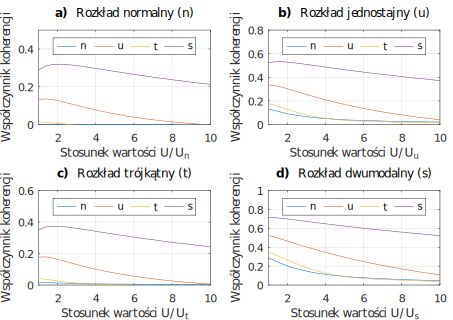
\includegraphics{obrazki/shapes}
\makecaption{fig:unc_shapefac}{Zależność wartości współczynnika koherencji w funkcji stosunku wartości niepewności rozszerzonej dla pary nieskorelowanych sygnałów błędów}
\end{center}
\end{figure}

Drugim analizowanym aspektem jest założenie wynikające z centralnego twierdzenia granicznego, wobec którego wraz ze wzrostem liczby sumowanych sygnałów kształt rozkładu sygnału wypadkowego dążyć będzie do kształtu rozkładu normalnego, jeśli sygnały te nie są skorelowane i nie występuje w nich żaden sygnał dominujący. Korektę wynikającą z opisywanych założeń zaproponowano w pracy~\cite{jakubiec_system} jako:
\begin{equation}
k_{i,j} = k_{j,i} = \frac{U_{i}^{2} + U_{j}^{2}}{\sum _{k = 0} ^{N-1} U_{k}^{2}} \label{eq:unc_cohercorrb}.
\end{equation}
Korekta ta zakłada, że współczynnik koherencji powinien być tym bardziej zbliżony do zera, im więcej istnieje źródeł błędów oraz im bardziej podobne są ich parametry. Należy zauważyć, że wraz ze wzrostem liczby sygnałów błędów cechujących się podobną wartością niepewności rozszerzonej wartość wyrażenia~\eqref{eq:unc_cohercorrb} dążyć będzie do zera tym szybciej, im bardziej zbliżone są wartości niepewności analizowanych sygnałów.

Biorąc pod uwagę współczynnik kształtu dla pary rozkładów o identycznych wartościach niepewności rozszerzonej, opisany równaniem~\eqref{eq:unc_shapertwo}, korektę wynikającą z dysproporcji pomiędzy wartościami niepewności rozszerzonych sumowanych sygnałów opisaną równaniem~\eqref{eq:unc_cohercorra} oraz korektę wynikającą z założeń centralnego twierdzenia daną zależnością~\eqref{eq:unc_cohercorrb}, otrzymuje się zależność umożliwiającą oszacowanie wartości współczynników koherencji dla $N$ nieskorelowanych sygnałów błędów w postaci:
\begin{equation}
h_{i,j} = h_{j,i} = s_{i,j} \cdot p_{i,j} \cdot k_{i,j} = s_{i,j} \sqrt{\frac{\min \emb{U_{i}, U_{j}}}{\max \emb{U_{i}, U_{j}}}} \left( \frac{U_{i}^{2} + U_{j}^{2}}{\sum _{k = 0} ^{N-1} U_{k}^{2}} \right) \label{eq:unc_coher}.
\end{equation}
Na podstawie przedstawionego równania istnieje możliwość budowy macierzy koherencji, wykorzystywanej do wyznaczenia wypadkowej wartości niepewności rozszerzonej dla analizowanych sygnałów błędów zgodnie z zależnością~\eqref{eq:unc_matrix}.

Należy zauważyć, że z uwagi na możliwość wyznaczenia wartości współczynników kształtu $s_{i,j}$ niezależnie od parametrów niepewności sygnałów błędów występujących w analizowanym torze pomiarowym, zaproponowana metoda jest możliwa do stosowania w czasie działania systemu również w przypadkach, gdy parametry sygnałów ulegają zmianie. Wadą przedstawionego rozwiązania jest konieczność wstępnego wyznaczenia wartości współczynników kształtu dla wszystkich rodzajów rozkładów sygnałów błędów występujących w analizowanym torze pomiarowym. Dodatkowo, ze względu na uproszczoną formę równania~\eqref{eq:unc_cohercorra}, która nie oddaje w pełni charakteru zależności przedstawionych na rysunku~\ref{fig:unc_shapefac}, wartości oszacowanych współczynników koherencji mogą być obarczone błędem, co w efekcie będzie miało wpływ na pojawienie się błędu oszacowania wartości wypadkowej niepewności rozszerzonej.

Ostatnim wymagającym komentarza przypadkiem jest przypadek, w którym istnieją korelacje pomiędzy analizowanymi sygnałami. Zgodnie z właściwościami macierzy koherencji elementy tej macierzy, podobnie jak elementy macierzy korelacji stosowanej w równaniu~\eqref{eq:var_matrix}, przyjmować mogą wartości z zakresu $<-1;1>$. Dla pełnej dodatniej korelacji wartość współczynnika koherencji wynosić będzie $1$, natomiast dla pełnej ujemnej korelacji wartość ta wyniesie $-1$~\cite{jakubiec_redmono}. W pozostałych przypadkach, zgodnie z informacjami przytoczonymi w poprzedniej części podrozdziału, wartość współczynnika koherencji wynikać będzie z wypadkowych parametrów kształtu splatanych rozkładów oraz współczynnika korelacji. Wobec powyższych nie jest możliwe oszacowanie wartości tego współczynnika stosując metody podobne do zaproponowanych w równaniach od~\eqref{eq:unc_shapertwo} do~\eqref{eq:unc_cohercorrb}. W omawianych sytuacjach, do wyznaczania wartości współczynników koherencji, zastosować należy metodę opisaną w pracy~\cite{jakubiec_reductive}. Inną drogą może być również przeprowadzenie analizy z osobna dla grup skorelowanych sygnałów, a następnie wykorzystanie wyznaczonych parametrów w równaniu~\eqref{eq:unc_matrix}.

Aby zweryfikować zasadność przedstawionych zależności oraz możliwość aplikacji zaproponowanej metody, przeprowadzono eksperyment metodą Monte-Carlo, którego celem było porównanie wartości niepewności rozszerzonej $U_{s}$ uzyskiwanej na drodze eksperymentu, zgodnie z instrukcją~\cite{jcgm_montecarlo}, oraz wartości $U_{c}$ uzyskiwanych zgodnie z równaniem~\eqref{eq:unc_matrix} dla współczynników koherencji wyznaczanych na podstawie równania~\eqref{eq:unc_coher}. Błąd względny $\delta_{U}$ oszacowania wartości niepewności rozszerzonej, wyrażony w procentach, będzie zatem definiowany w postaci:
\begin{equation}
\delta_{U} =  \frac{U_{c} - U_{s}}{U_{s}} \cdot 100\% \label{eq:unc_error}.
\end{equation}
W ramach eksperymentu generowano $N$ niezależnych sygnałów, których realizacje pobierane były z populacji o rozkładach $c_{i}$ i parametrach niepewności rozszerzonej $U_{i}$, których kolejne realizacje sumowano:
\begin{equation}
e_{\Sigma} \emb{k} = \sum _{i=0} ^{N-1} e_{i} \emb{k} \label{eq:unc_testsignal}.
\end{equation}
Dla uzyskanego sygnału, składającego się ze stu tysięcy próbek, wyznaczano niepewność rozszerzoną $U_{s}$ zgodnie z równaniem~\eqref{eq:unc_summation} oraz wartość $U_{c}$ oszacowaną na podstawie równania~\eqref{eq:unc_matrix} w celu wyznaczenia zgodnie z równaniem~\eqref{eq:unc_error} względnego błędu oszacowania wartości analizowanej wielkości. Opisywany proces powtarzano sto tysięcy razy, przy czym wartość $N$ pobierana była dla każdej iteracji z populacji danej przedziałem $<3,9>$ o jednakowym prawdopodobieństwie uzyskania każdej z wartości. Populacje kolejnych sygnałów $e_{i}$ stanowiły losowo kombinację rozkładów: normalnego, jednostajnego, trójkątnego i dwumodalnego, natomiast wartości niepewności rozszerzonej $U_{i}$ losowane były z przedziału $<U_{min};U_{max}>$ o jednakowym prawdopodobieństwie uzyskania każdej z wartości. Aby zweryfikować, w jakim stopniu zaproponowany w równaniu~\eqref{eq:unc_cohercorra} współczynnik korekty wpłynął na skuteczność opisanej w równaniu~\eqref{eq:unc_matrix} metody, eksperyment przeprowadzono dwukrotnie: stosując wartości współczynników koherencji wyznaczanych zgodnie z równaniem~\eqref{eq:unc_cohercorra} oraz po raz drugi, przyjmując wartość $p_{i,j} = 1$ dla dowolnej kombinacji $i$ oraz $j$. Na podstawie uzyskiwanych realizacji błędu opisanego równaniem~\eqref{eq:unc_error} sporządzano histogramm na którego podstawie oszacowano niepewność rozszerzoną analizowanej wielkości.

Ze względu na dużą zmienność parametrów sumowanych sygnałów zaproponowany eksperyment powinien w sposób miarodajny określić typową rozbieżność pomiędzy rzeczywistą, a oszacowaną za pomocą omawianej metody wartością niepewności rozszerzonej. Rysunek~\ref{fig:hist_reductive} przedstawia uzyskane histogramy względnego błędu oszacowania wypadkowej wartości niepewności rozszerzonej, natomiast w tabeli~\ref{tab:comp_reductive} przedstawiono porównanie uzyskanych wartości niepewności rozszerzonej błędu oszacowania wartości wypadkowej niepewności rozszerzonej w zależności od stosowania korekty zaproponowanej w równaniu~\eqref{eq:unc_cohercorra}, wyznaczone zgodnie z~\cite{jcgm_guide, jcgm_montecarlo}. Analizując wyniki przeprowadzonego eksperymentu zauważyć można, że wprowadzenie proponowanej korekty powoduje zmniejszenie szacowanej wartości niepewności rozszerzonej, a także zmniejszenie rozrzutu względnego błędu oszacowania tej wielkości. W efekcie możliwe jest oszacowanie wartości wypadkowej niepewności rozszerzonej z błędem względnym mieszczącym się w przedziale $\pm 5\%$.

\begin{table}[htb!]
\begin{center}
\makecaption{tab:comp_reductive}{Zestawienie wartości niepewności względnego błędu szacowania wypadkowej wartości niepewności rozszerzonej w zależności od stosowania zaproponowanej w pracy korekty współczynnika kształtu}
\begin{tabular}[c]{| c | S[table-format = +1.2] | S[table-format = +1.2] | S[table-format = +1.2] | S[table-format = +1.2] | S[table-format = +1.2] | S[table-format = +1.2] | S[table-format = +1.2] | S[table-format = +1.2] |} \hline
\textbf{$U_{i}$} & \multicolumn{2}{c|}{\textbf{a) $<1;3>$}} & \multicolumn{2}{c|}{\textbf{b) $<1;6>$}} & \multicolumn{2}{c|}{\textbf{c) $<1;10>$}} & \multicolumn{2}{c|}{\textbf{d) $<1;20>$}} \\ \hline
\textbf{$\delta_{U}$} & \textbf{$U_{-}$} & \textbf{$U_{+}$} & \textbf{$U_{-}$} & \textbf{$U_{+}$} & \textbf{$U_{-}$} & \textbf{$U_{+}$} & \textbf{$U_{-}$} & \textbf{$U_{+}$} \\ \hline
Z korektą   & -2.23 & +4.83 & -2.43 & +4.59 & -2.54 & +4.52 & -2.62 & +4.45 \\ \hline
Bez korekty & -1.14 & +7.96 & -1.13 & +8.69 & -1.09 & +8.80 & -1.13 & +8.86 \\ \hline
\end{tabular}
\end{center}
\end{table}

\begin{figure}[htb!]
\begin{center}
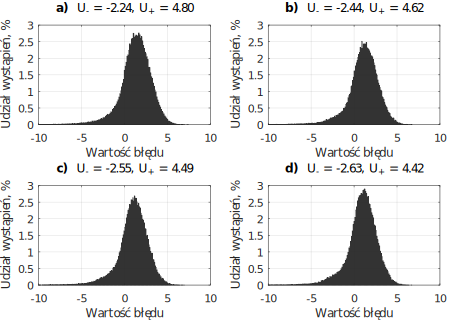
\includegraphics{obrazki/hist_reductive}
\makecaption{fig:hist_reductive}{Histogramy względnego błędu oszacowania wypadkowej wartości niepewności rozszerzonej dla zaproponowanej w pracy metody odpowiadające danym zestawionym w tabeli~\ref{tab:comp_reductive}}
\end{center}
\end{figure}

Analizując przedstawione dotychczas zależności zauważyć można, że sposób opisu niedokładności wyniku pomiaru zależeć będzie w dużej mierze od potrzeb projektanta toru pomiarowego oraz od specyfiki zakłócających proces pomiaru zjawisk. Opis wykorzystujący wariancję sygnału błędu wydaje się bardziej przystępny i mniej skomplikowany, a dodatkowo wielkość ta może być utożsamiana z mocą sygnału~\cite{proakis_dsp}. Opis wykorzystujący niepewność rozszerzoną będzie jednak bardziej precyzyjny, ze względu na informacje odnośnie prawdopodobieństwa wystąpienia danej wartości realizacji sygnału błędu, natomiast wymaga on większego zaangażowania w proces wyznaczania ostatecznej wartości tej wielkości. W odpowiednich okolicznościach, jeżeli spełnione są warunki związane z centralnym twierdzeniem granicznym, opis bazujący na wariancji sygnału błędu może być w łatwy sposób przeniesiony na opis związany z niepewnością rozszerzoną~\cite{jcgm_guide}.

Wyznaczone zgodnie z metodą redukcyjnej arytmetyki interwałowej szacowane wartości niepewności rozszerzonej mogą w niewielkim stopniu odbiegać od wartości rzeczywistych, co opisano w~\cite{jakubiec_arithmetic, jakubiec_model}. Zaproponowana w równaniu~\eqref{eq:unc_cohercorra} korekta zmniejsza omawiane różnice, zapewniając jednocześnie niski stopnień skomplikowania obliczeń oraz względny błąd oszacowania wypadkowej wartości niepewności rozszerzonej nieprzekraczający $\pm 5\%$ prawidłowej wartości tej wielkości. Można zatem stwierdzić, że zaproponowana w pracy metoda szacowania wypadkowej wartości niepewności rozszerzonej jest zasadna z punktu widzenia przyjętych założeń. Ponadto, ze względu na niską złożoność obliczeń, metoda ta może być stosowana w przypadkach, gdzie liczba analizowanych sygnałów oraz ich parametry ulegają zmianie.

\section{Algorytm jako fragment toru pomiarowego}

Podczas opisu właściwości cyfrowej części toru pomiarowego przedstawiono przypadek ogólny, w którym analizowany obiekt przetwarzał kolejne próbki sygnału wejściowego na próbki sygnału wyjściowego zgodnie z odpowiadającą mu transmitancją i funkcją przetwarzania. Algorytmy stosowane w torach pomiarowych mogą generować wiele wielkości wyjściowych, pobierając w tym celu określoną liczbę próbek wielkości wejściowych. W przypadku, gdy wyjście analizowanego obiektu stanowi $M$ próbek wielkości wyjściowych wyznaczanych na podstawie $N$ próbek wielkości wejściowych, a funkcja przetwarzania oraz transmitancja tego obiektu są liniowe i niezmienne w czasie, działanie obiektu przedstawić można w postaci równania~\cite{jakubiec_algorithms, jakubiec_single}:
\begin{equation}
\begin{bmatrix}
X \emb{0}   \\
X \emb{1}   \\
\vdots      \\
X \emb{M-1}
\end{bmatrix}
=
\begin{bmatrix}
a_{0, 0}   &   a_{0, 1} &   \cdots   &   a_{0, N-1}      \\
a_{1, 0}   &   \ddots   &            &   a_{1, N-1}      \\
\vdots     &            &   \ddots   &   \vdots          \\
a_{M-1, 0} &   \cdots   &   \cdots   &   a_{M-1, N-1}
\end{bmatrix}
\begin{bmatrix}
x \emb{0}   \\
x \emb{1}   \\
\vdots      \\
x \emb{N-1}
\end{bmatrix}
\label{eq:alg_out_mat},
\end{equation}
gdzie $a_{i,j}$ to kolejne współczynniki macierzy transformacji, $X(i)$ to kolejne wielkości wejściowe, natomiast $x(j)$ to kolejne wielkości wejściowe analizowanego algorytmu. Równanie~\eqref{eq:alg_out_mat} można przedstawić również w postaci iloczynu~\cite{jakubiec_algorithms}:
\begin{equation}
\mathbf{X} = \mathbf{A} \cdot \mathbf{x} \label{eq:alg_out_mul},
\end{equation}
gdzie $\mathbf{X}$ jest wektorem wielkości wyjściowych, $\mathbf{A}$ macierzą transformacji oraz $\mathbf{x}$ wektorem wielkości wejściowych. Wobec powyższych zależności, pojedynczą wielkość wyjściową algorytmu przedstawić można w postaci:
\begin{equation}
X \emb{i} = a_{i, 0} x \emb{0} + a_{i, 1} x \emb{1} + \hdots + a_{i, N-1} x \emb{N-1} = \sum _{j = 0} ^{N-1} a_{i,j} x \emb{j} \label{eq:alg_out_single}.
\end{equation}
Na podstawie równania~\eqref{eq:alg_out_single} zauważyć można, że analizowany obiekt stanowi zbiór filtrów o skończonej odpowiedzi impulsowej \enquote{FIR} (ang. \enquote{Finite Impulse Response}). Przedstawione metody analizy będą zatem przypominały metody analizy opisywanego typu filtru~\cite{mehrnia_fir}. Przedstawione założenie odnośnie stałej transmitancji algorytmu implikuje niezmienność wartości elementów macierzy transformacji analizowanego algorytmu. W przypadku, gdy istnieje konieczność analizy algorytmu o zmiennej transmitancji, przy zmianie tej transmitancji należy każdorazowo wyznaczyć wartości wszystkich wielkości od niej zależnych.

Jako, że w procesie przetwarzania danych stosuje zwykle gotowe algorytmy, zaimplementowane np. w środowiskach \enquote{GNU Octave} czy \enquote{Matlab}~\cite{pruuvsa_dwt, lee_pywavelets}, wartości współczynników macierzy transformacji $\mathbf{A}$ stosowanej w równaniach~\eqref{eq:alg_out_mat} oraz~\eqref{eq:alg_out_mul} mogą nie być znane. Jeżeli znana jest transmitancja $H_{i}(z)$ dla kolejnych wielkości wyjściowych, wyznaczenie wartości współczynników macierzy transformacji odbywać się będzie poprzez przekształcenie tej transmitancji na postać zgodną z równaniem~\eqref{eq:alg_out_single}, przy czym zabieg ten nie jest konieczny. Analiza właściwości metrologicznych w omawianym przypadku przebiegać może identycznie, jak miało to miejsce w przypadku cyfrowego fragmentu toru pomiarowego, natomiast wyznaczenie wartości współczynników macierzy transformacji przy znajomości transmitancji algorytmu pozwoli w pewnym stopniu uprościć analizę, co przedstawiono w dalszej części podrozdziału. Drugim przypadkiem jest sytuacja, w której wartości współczynników mogą być wyznaczone analitycznie za pomocą odpowiednich zależności, opisujących stosowany algorytm, jak ma to zwykle miejsce w przypadku algorytmów dyskretnej transformacji falkowej~\cite{vonesch_dbbasics}. Ostatnim analizowanym w pracy przypadkiem jest sytuacja, w której dostępna jest implementacja stosowanego algorytmu, natomiast nie jest znana jego struktura numeryczna~\cite{misiti_matlabwav}.

Jeżeli analizowany algorytm jest liniowy oraz jego transmitancja jest liniowa i niezmienna w czasie, związek pomiędzy transmitancją $H_{i}(z)$ dla $i$-tej wielkości wyjściowej oraz $i$-tym wierszem macierzy transformacji $\mathbf{A}$ może być opisany równaniem:
\begin{equation}
H_{i} \emb{z} = a_{i, 0} + a_{i, 1} z^{-1} + \hdots + a_{i, N-1} z^{-N+1} = \sum _{k = 0} ^{N-1} a_{i, k} z^{-k} \label{eq:alg_trans_single}.
\end{equation}
Przedstawiona zależność umożliwia wyznaczenie wartości współczynników macierzy transformacji przy znajomości transmitancji wielkości wyjściowych algorytmu oraz wyznaczenie transmitancji tych wielkości przy znajomości wartości macierzy transformacji tego algorytmu. W celu wyznaczenia transmitancji $H_{i}(z)$ dla $i$-tej wielkości wyjściowej algorytmu w dziedzinie pulsacji, odpowiedniej dla okresu próbkowania $T_{p}$, należy przyjąć w równaniu~\eqref{eq:alg_trans_single} założenie gdzie $z = e^{j\omega T_{p}}$~\cite{proakis_dsp}.

Identyfikacja wartości współczynników macierzy transformacji w przypadku istniejącego algorytmu polega na wyznaczaniu odpowiedzi tego algorytmu dla wektora wielkości wejściowych o wartościach zgodnych z równaniem~\cite{jakubiec_algorithms, jakubiec_system}:
\begin{equation}
x \emb{n} =
\begin{cases}
	1 & $gdy$~n = j \\
	0 & $gdy$~n \neq j
\end{cases}
\label{eq:wt_ident},
\end{equation}
przy czym uzyskany wektor wielkości wyjściowych stanowi $j$-tą kolumnę macierzy transformacji tego algorytmu. Przedstawioną operację należy wykonać dla wszystkich kolumn macierzy transformacji, a zatem dla $j$ w przedziale $<0;N-1>$. Opisana metoda jest uniwersalna, przy czym wymaga ona, aby identyfikowany algorytm spełniał założenia przedstawione na początku podrozdziału.

Przedstawione dotychczas zależności podkreślają ścisły związek pomiędzy transmitancją kolejnych wielkości wyjściowych algorytmu oraz wartościami macierzy transformacji. Należy zauważyć, że z punktu widzenia zaproponowanego w pracy modelu, rozpatrywany algorytm mógłby być analizowany jako kilka obiektów cyfrowej części toru pomiarowego, przetwarzających te same wielkości wejściowe $x(i)$ na odpowiednie wielkości wyjściowe $X_{j}(i)$. Przedstawienie algorytmu w postaci macierzowej pozwala natomiast ujednolicić analizę i sprowadzić ją do zastąpienia opisywanej grupy obiektów jednym obiektem. Mnogość sposobów wyznaczania wartości elementów macierzy transformacji stanowi dodatkowy, cenny walor proponowanej metody analizy.

Aby ustalić związek pomiędzy sygnałami błędów wielkości wejściowych, a sygnałami błędów wielkości wyjściowych analizowanego algorytmu, należy rozważyć proces wyznaczania wartości pojedynczej wielkości wyjściowej tego obiektu. Zakładając, że wielkości wejściowe algorytmu są obarczone realizacjami sygnałów błędów o charakterze addytywnym zgodnie z zależnością:
\begin{equation}
\tilde{x} \emb{i} = \dot{x} \emb{i} + e_{x,s} \emb{i} + e_{x,d} \emb{i} + e_{x,r} \emb{i} = \dot{x} \emb{i} + e_{x,\Sigma} \emb{i} \label{eq:alg_inputval},
\end{equation}
gdzie $e_{x,s}(i)$ oznacza błąd statyczny, $e_{x,d}(i)$ błąd dynamiczny oraz $e_{x,r}(i)$ błąd losowy wielkości wejściowej, istnieje możliwość osobnej analizy wyniku realizacji algorytmu dla idealnych wartości wielkości wejściowych oraz dla wymienionych sygnałów błędów. Sygnał błędu $e_{X,p}(i)$ propagowanego z wejścia na wyjście analizowanego algorytmu można zatem opisać zgodnie z równaniem~\eqref{eq:alg_out_single} w postaci:
\begin{equation}
e_{X,p} \emb{i} = a_{i, 0} e_{x,\Sigma} \emb{0} + a_{i, 1} e_{x,\Sigma} \emb{1} + \hdots + a_{i, N-1} e_{x,\Sigma} \emb{N-1} = \sum _{j = 0} ^{N-1} a_{i,j} e_{x,\Sigma} \emb{j} \label{eq:alg_outerr}.
\end{equation}
Realizacja propagowanego sygnału błędu $e_{X,p}(i)$ stanowi zatem kombinację liniową współczynników $i$-tego wiersza macierzy transformacji oraz wektora realizacji sygnału błędu wielkości wejściowych algorytmu.

Dla sygnałów błędów o charakterze statycznym, ze względu na fakt że wartość realizacji tych sygnałów jest niezmienna w obrębie pojedynczego okna pomiarowego, równanie~\eqref{eq:alg_outerr} można uprościć i zapisać w postaci:
\begin{equation}
e_{X,sp} \emb{i} = a_{i, 0} e_{x,s} \emb{k} + a_{i, 1} e_{x,s} \emb{k} + \hdots + a_{i, N-1} e_{x,s} \emb{k} = e_{x,s} \emb{k} \sum _{j = 0} ^{N-1} a_{i, j} \label{eq:alg_outerr_stat},
\end{equation}
gdzie $e_{x,s}(k)$ jest błędem statycznym wielkości wejściowej dla $k$-tego okna pomiarowego, natomiast $e_{X,sp}(i)$ błędem statycznym propagowanym wielkości wyjściowej algorytmu. Powtarzając proces wyznaczania wartości wielkości wyjściowej algorytmu wielokrotnie, dla różnych numerów okna pomiarowego realizacje sygnału błędu statycznego mogą przyjmować różne wartości. W takim przypadku wyjściowy błąd statyczny również można rozpatrywać w kategoriach probabilistycznych, a jego wariancję opisać można równaniem uwzględniającym wariancję sygnału wejściowego błędu statycznego:
\begin{equation}
\sigma_{X,sp}^{2} \emb{i} = \sigma_{x,s}^{2} \left( a_{i, 0} + a_{i, 1} + \hdots + a_{i, N-1} \right)^{2} = \sigma_{x,s}^{2} \left( \sum _{j = 0} ^{N-1} a_{i, j} \right)^{2} \label{eq:alg_outvar_stat}.
\end{equation}
Należy zauważyć, że kształt rozkładu sygnału wyjściowego błędu statycznego będzie identyczny, jak kształt rozkładu sygnału błędu statycznego na wejściu algorytmu.

Dla sygnałów błędów dynamicznych należy przeprowadzić analizę zgodnie z metodologią przedstawioną w poprzedniej części rozdziału, wykorzystując znajomość transmitancji $H_{i}(z)$ odpowiedniej dla analizowanej wielkości wyjściowej algorytmu. Identycznie, jak w przypadku równania~\eqref{eq:mid_disc_err_dyn_prop}, wyznaczyć należy wypadkowe amplitudy oraz przesunięcia w fazie kolejnych harmonicznych sygnału propagowanego błędu dynamicznego, a następnie wykorzystać należy równania od~\eqref{eq:dyn_harm} do~\eqref{eq:dyn_corr} w celu wyznaczenia wariancji analizowanych sygnałów. Na podstawie wskazanych zależności, wariancję $\sigma_{X,dp}^{2}(\omega)$ pojedynczej harmonicznej sygnału propagowanego błędu dynamicznego $e_{x,d}(i)$ wyznaczyć można zgodnie z zależnością:
\begin{equation}
\sigma_{X,dp}^{2} \emb{\omega} = \frac{1}{2} E_{x,e}^{2} \emb{\omega} \left| H \emb{e^{j\omega T_{p}}} \right|^{2} \label{eq:alg_outvar_dyn},
\end{equation}
gdzie $E_{x,e}(\omega)$ jest amplitudą analizowanej harmonicznej sygnału błędu dynamicznego $e_{x,d}(i)$ o pulsacji $\omega$, natomiast $T_{p}$ okresem próbkowania wielkości wejściowych algorytmu.

Sygnały błędów niedeterministycznych propagowane są przez analizowany algorytm w sposób identyczny, jak miało to miejsce w przypadku cyfrowej części toru pomiarowego. W ogólnym przypadku można zatem wykorzystać zależność~\eqref{eq:mid_disc_var_omega} w celu określenia wariancji $\sigma_{X,rp}^{2}(\omega)$ propagowanego błędu losowego $e_{x,r}(i)$ w funkcji pulsacji. Wyznaczenie średniej wartości omawianej wielkości może odbywać się zgodnie z równaniem~\eqref{eq:mid_disc_var_rand}, przy czym należy wyznaczać ją dla przedziału $\omega \in <0; \frac{\omega_{p}}{2}>$. Jeżeli analizowany sygnał błędu losowego $e_{x,r}(i)$ cechuje się stałą widmową gęstością mocy, to obliczenia można uprościć stosując do wyznaczenia wartości wariancji losowego sygnału błędu na wyjściu algorytmu zależność~\cite{jakubiec_system}:
\begin{equation}
\sigma_{rp}^{2} \emb{i} = a_{i, 0}^{2} \sigma_{x,r}^{2} + a_{i, 1}^{2} \sigma_{x,r}^{2} + \hdots + a_{i, N-1}^{2} \sigma_{x,r}^{2} = \sigma_{x,r}^{2} \sum _{j=0} ^{N-1} {a_{i, j}^{2}} \label{eq:alg_outvar_rand}.
\end{equation}
Niezależnie od zastosowanego sposobu obliczeń, każda metoda dostarcza identyczne wyniki, jeżeli tylko została zastosowana w odpowiednich dla niej okolicznościach.

Znajomość wartości kolejnych elementów macierzy transformacji pozwala na podstawie równań~\eqref{eq:alg_outvar_stat} oraz~\eqref{eq:alg_outvar_rand} wprowadzić dodatkowe wielkości, przedstawione następującymi zależnościami~\cite{jakubiec_algorithms}:
\begin{gather}
A_{i,s} = \sum _{j = 0} ^{N-1} a_{i, j} \label{eq:alg_trans_stat}, \\
A_{i,r} = \sqrt{\sum _{j = 0} ^{N-1} a_{i, j}^{2}} \label{eq:alg_trans_rand},
\end{gather}
gdzie $A_{i,s}$ jest współczynnikiem przenoszenia dla błędów statycznych, natomiast jest $A_{i,r}$ współczynnikiem przenoszenia dla błędów losowych $i$-tej wielkości wyjściowej analizowanego algorytmu. Wyznaczenie wartości opisanych współczynników umożliwi wyznaczenie wariancji kolejnych błędów losowych oraz statycznych, a dodatkowo będzie stanowiło informacje, w jaki sposób analizowany algorytm przenosi z wejścia na wyjście określony rodzaj błędu. Można zauważyć, że dla niskich wartości współczynnika przenoszenia (tj. $A_{i} < 1$) kolejne błędy wielkości wejściowych będą tłumione (wariancja błędu wielkości wyjściowej będzie mniejsza, niż wariancja błędów wielkości wejściowych). Odwrotna sytuacja będzie miała miejsce w przypadku dużych wartości współczynnika (tj. $A_{i} > 1$). Wobec powyższych zapisać można:
\begin{gather}
\sigma_{X,sp}^{2} = \sigma_{x,s}^{2} A_{i,s}^{2} \label{eq:alg_outvar_trans_stat}, \\
\sigma_{X,rp}^{2} = \sigma_{x,r}^{2} A_{i,r}^{2} \label{eq:alg_outvar_trans_rand}.
\end{gather}
Należy zauważyć, że stosowanie równania~\eqref{eq:alg_outvar_trans_rand} pozwala oszacować średnią widmową gęstość mocy analizowanego sygnału błędu tylko w przypadku, gdy sygnał ten cechuje się stałą widmową gęstością mocy. Wyznaczenie średniej wariancji sygnału błędu losowego będzie zasadne dla przypadków, gdzie dalsza analiza wpływu kolejnych obiektów na rozważany sygnał błędu nie będzie prowadzona, zatem gdy obiekt stanowi ostatnią część toru pomiarowego. W innym wypadku należy zastosować zależność~\eqref{eq:mid_disc_var_omega}.

Poza przenoszeniem przez algorytm błędów zawartych w wielkościach wejściowych na jego wyjście, algorytm wprowadza do wielkości wyjściowych błędy własne. W pracy przyjmuje się, że transmitancja algorytmu jest idealna, a zatem algorytm ten nie wprowadza do sygnału wyjściowego błędów własnych o charakterze deterministycznym. Wobec przedstawionego założenia, błędy własne algorytmu wynikają z niedokładności wyznaczenia współczynników algorytmu oraz z przeprowadzanych podczas obliczeń zaokrągleń. Ich wartości będą zatem uzależnione od wielu czynników, a ich analiza powinna odbywać się indywidualnie dla zaimplementowanego algorytmu.

Zakładając, że wyznaczanie wartości $i$-tej wielkości wyjściowej algorytmu odbywać się będzie wielokrotnie, błędy własne algorytmu opisywać można w kategorii probabilistycznej za pomocą związanej z nimi wariancji $\sigma_{X,rw}^{2}(i)$. Ze względu na fakt, że liczba operacji mnożenia i dodawania, odpowiedzialnych za powstawanie omawianej grupy błędów będzie duża ($N$ mnożeń oraz $N$ dodawań) zakładać można, że błąd ten będzie miał rozkład zbliżony do normalnego~\cite{jcgm_guide}. Należy jednak przeprowadzić odpowiedni eksperyment mający na celu identyfikacje opisywanych zależności, co przedstawiono na przykładzie w dalszej cześć pracy.

W przypadku, gdy na etapie identyfikacji wartości macierzy współczynników uzyskano wartości obarczone błędami, należy rozszerzyć analizę o przedstawienie konsekwencji tego zjawiska. W takim przypadku należy przeanalizować wprowadzany do wielkości wyjściowych dodatkowy błąd własny oraz wykonać analizę dla błędów własnych dynamicznych zgodnie z równaniem~\eqref{eq:mid_disc_err_dyn_self}. Identyczne kroki należy podjąć, jeżeli rzeczywista transmitancja algorytmu różni się od transmitancji wymaganej z punktu widzenia jego działania. Przedstawiony przypadek nie został rozważony w pracy, natomiast omawianą analizę przedstawia szczegółowo monografia~\cite{jakubiec_system}.

Zgodnie z przedstawionymi dotyczącymi proponowanego w pracy modelu błędu, zapisać można równania opisujące $i$-tą wielkość wyjściową $X(i)$ analizowanego algorytmu, będące podsumowaniem dotychczasowych rozważań:
\begin{gather}
\dot{X} \emb{i} = \sum _{j = 0} ^{N-1} \dot{a}_{i,j} \dot{x} \emb{j} \label{eq:alg_out_ideal}, \\
\tilde{X} \emb{i} = \dot{X} \emb{i} + e_{X,\Sigma} \emb{i} \label{eq:alg_out_real},
\end{gather}
przy czym wypadkowy sygnał błędu $e_{X,\Sigma}(i)$ związany z tą wielkością opisać można jako:
\begin{equation}
e_{X,\Sigma} \emb{i} = e_{X,w} \emb{i} + e_{X,p} \emb{i} \label{eq:alg_out_err},
\end{equation}
natomiast sygnały błędów własnego $e_{X,w}(i)$ oraz propagowanego $e_{X,p}(i)$ przedstawić można w postaci sumy składowych tych sygnałów:
\begin{gather}
e_{X,w} \emb{i} = e_{X,sw} \emb{i} + e_{X,dw} \emb{i} + e_{X,rw} \emb{i} \label{eq:alg_out_err_self}, \\
e_{X,p} \emb{i} = e_{X,sp} \emb{i} + e_{X,dp} \emb{i} + e_{X,rp} \emb{i} \label{eq:alg_out_err_prop},
\end{gather}
Rozważając podział sygnałów błędów ze względu na charakter ich realizacji, równania~\eqref{eq:alg_out_err_self} oraz~\eqref{eq:alg_out_err_prop} zapisać można również w postaci:
\begin{gather}
e_{X,s} \emb{i} = e_{X,sw} \emb{i} + e_{X,sp} \emb{i} \label{eq:alg_out_err_stat}, \\
e_{X,d} \emb{i} = e_{X,dw} \emb{i} + e_{X,dp} \emb{i} \label{eq:alg_out_err_dyn}, \\
e_{X,r} \emb{i} = e_{X,rw} \emb{i} + e_{X,rp} \emb{i} \label{eq:alg_out_err_rand}.
\end{gather}
Dokładna postać wymienionych w równaniach od~\eqref{eq:alg_out_err_self} do~\eqref{eq:alg_out_err_rand} sygnałów błędów zależeć będzie od analizowanego algorytmu. Należy zatem wykorzystać przedstawione w bieżącym rozdziale zależności w celu określenia wzajemnych relacji pomiędzy sygnałami błędów na wejściu i wyjściu algorytmu oraz zdefiniować istotne z punktu widzenia właściwości metrologicznej sygnały błędów własnych analizowanego algorytmu. Przykład aplikacji omawianej metody przedstawiono w dalszej części pracy.

Wobec powyższych założeń, w celu wyznaczenia wariancji $\sigma_{X,\Sigma}^{2}(i)$ wypadkowego błędu $e_{X,\Sigma}(i)$ dla $i$-tej wielkości wyjściowej analizowanego algorytmu należy wykorzystać zależność~\eqref{eq:var_matrix}. Wyznaczenie niepewności rozszerzonej w przypadku omawianego sygnału może być natomiast przeprowadzone zgodnie z zależnością~\eqref{eq:unc_matrix}. W przedstawionych równaniu uwzględnić należy parametry wszystkich zidentyfikowanych sygnałów błędów, obecnych w sygnale związanym z analizowaną wielkością wyjściową.

Należy zauważyć, że ze względu na właściwości stosowanej w pracy metody szacowania wypadkowej wartości niepewności rozszerzonej, najbardziej korzystnym podejściem jest analiza każdego sygnału błędu z osobna. Omówiona właściwość wynika z zaproponowanego sposobu szacowania wartości współczynników koherencji, opisanego równaniem~\eqref{eq:unc_coher}, wymagającego znajomości wartości współczynników kształtu dla analizowanych par rozkładów. Należy zauważyć, że w wyniku sumowania kolejnych sygnałów błędów i analizy wypadkowego sygnału, wypadkowy sygnał może cechować się rozkładem o nietypowym kształcie~\cite{auth_electronics, zhang_pdp}.

\section{Błędy spowodowane opóźnieniami}

Przeprowadzone rozważania nie poruszały problemu opóźnień w systemach pomiarowo-sterujących, a zatem nie brano w nich pod uwagę sygnałów błędów związanych z możliwymi opóźnieniami. Mimo, że tematyka pracy nie obejmuje przedstawionego zagadnienia, warto jednak zauważyć, że zaproponowany model błędu może być z dopasowany do możliwości analizy właściwości i wpływu tych zjawisk na niedokładność wyznaczania wartości wielkości wyjściowych rozważanego toru pomiarowego. Należy w takim przypadku uwzględnić w modelu dodatkowy sygnał błędu, który definiować można zgodnie z metodą zaproponowaną w pracach~\cite{wymyslo_delay, jakubiec_system} oraz uwzględnić wpływ analizowanego zjawiska na propagację przez obiekt pozostałych sygnałów błędów.

Z punktu widzenia zaproponowanego modelu, zjawisko opóźnień w systemie opisać można jako dodatkowe przesunięcie w fazie składowych przetwarzanego sygnału oraz sygnałów błędów deterministycznych, będące iloczynem pulsacji analizowanej harmonicznej i wartości realizacji błędu opóźnienia. Omawiany sygnał mógłby być zdefiniowany w przypadku przetwornika cyfrowo-analogowego jako dodatkowa harmoniczna sygnału błędu dynamicznego własnego:
\begin{equation}
\begin{split}
e_{x,tw} \emb{i}
= ~ & E_{y,o} \emb{\omega} \sin \left( \omega \emb{i T_{p} + t_{x} \emb{i}} + \varphi_{y,o} \emb{\omega} \right) \\
= ~ & E_{y,o} \emb{\omega} \sin \left( \omega iT_{p} + \varphi_{y,o} \emb{\omega} + \varphi_{x,t} \emb{\omega, i} \right) 
\end{split}
\label{eq:tim_err_self},
\end{equation}
gdzie $t_{x}(i)$ stanowi realizację opóźnienia dla $i$-tej wielkości wyjściowej analizowanego obiektu przetwarzającego ciągły w czasie sygnał $y(t)$ na jego dyskretne próbki $x(i)$, natomiast $\varphi_{x,t}(\omega, i)$ jest realizacją przesunięcia fazowego analizowanej harmonicznej dla $i$-tej wielkości wyjściowej i wynosi:
\begin{equation}
\varphi_{x,t} \emb{\omega, i} = \omega t_{x} \emb{i} \label{eq:tim_err_phi}.
\end{equation}
Należy zaznaczyć, że w przypadku analizy opóźnień równania opisujące propagowany przez związany z opóźnieniami obiekt sygnał błędu dynamicznego również musiały by zostać zmodyfikowane z uwzględnieniem wprowadzanego opóźnienia.

Przedstawiona w równaniu~\eqref{eq:tim_err_self} koncepcja stanowi jedynie pojedynczy przypadek analizy opóźnienia w działaniu fragmentu toru pomiarowego. Celem poruszenia przedstawionego zagadnienia, mimo że nie obejmuje ono tematyki pracy, było podkreślenie możliwości dalszego rozwoju zaproponowanego modelu błędu o możliwość analizy kolejnych źródeł niedokładności wyznaczania wartości wielkości wyjściowych torów pomiarowych. Przedstawione zagadnienie może stanowić dalsze prace badawcze.

\section{Podsumowanie przedstawionych zależności}

W poprzednich częściach rozdziału przedstawiono modele kolejnych fragmentów toru pomiarowego, które opisywały związki pomiędzy sygnałami błędów na wejściu i wyjściu analizowanego obiektu oraz wskazywały rolę tego obiektu we wprowadzaniu do sygnału wyjściowego sygnałów błędów własnych. Zaproponowany model wprowadzał podział na statyczne i dynamiczne właściwości obiektu, które opisywane były transmitancją i funkcją przetwarzania obiektu. Opisane zgodnie z zaproponowanym modelem fragmenty toru pomiarowego, które zostały ze sobą połączone kaskadowo oraz cechują się addytywną i liniową funkcją przetwarzania, opisać można pojedynczym obiektem o wypadkowych właściwościach analizowanych fragmentów.

Przedstawiony model oceny dokładności wyniku pomiaru zakłada, że obecne w sygnale pomiarowym sygnały błędów cechują się symetrycznymi rozkładami o zerowej wartości oczekiwanej. W przypadku, gdy wartość oczekiwana realizacji sygnału błędu jest niezerowa, błąd ten posiada składową systematyczną, którą należy skorygować w ostatecznym wyniku pomiaru. Jeżeli nie jest spełnione założenie odnośnie symetrii rozkładów składanych błędów, to do określenia rozkładu błędu wynikowego należy stosować metodę analityczną bazującą na wyznaczeniu splotu składanych funkcji gęstości prawdopodobieństwa lub wykorzystać metodę Monte-Carlo, która jest zwykle bardziej przystępna ze względu na mniejszy stopień skomplikowania~\cite{janssen_montecarlo, roj_annuncertainty}.

Zastosowanie przedstawionego modelu błędu wymaga ze strony projektanta pomiarowego wiedzy na temat działania i właściwości kolejnych jego fragmentów. Mimo, że tematykę pracy stanowi analiza właściwości metrologicznych algorytmów dyskretnej transformacji falkowej, przedstawienie modelu błędu fragmentu toru pomiarowego stanowiącego źródło danych tego algorytmu było konieczne ze względu na określenie jego udziału w procesie przetwarzania danych pomiarowych. Jak wykazano w poprzednich pracach~\cite{auth_window, auth_electronics}, w wielu przypadkach algorytmy te przetwarzają jedynie sygnały błędów zawarte w wielkościach wejściowych, a wprowadzane przez nie błędy własne są pomijalnie małe. Wobec powyższych rola obiektów stanowiących źródło przetwarzanych przez analizowany algorytm danych będzie kluczowa w ocenie właściwości metrologicznych całości toru pomiarowego.

Zaproponowany model błędu umożliwia rozszerzenie analizy o dodatkowe sygnały wypływające na niedokładność wyznaczania wartości wielkości wyjściowych rozważanego toru pomiarowego. Należy w tym celu zdefiniować źródło takiego sygnału oraz wyznaczyć jego parametry. Sygnał ten błędzie następnie przetwarzany przez kolejne fragmenty toru pomiarowego, zgodnie z przedstawionymi zależnościami. Przedstawione podejście stanowi cenny walor proponowanego modelu błędu oraz umożliwia podjęcie kolejnych rozważań odnośnie dodatkowych źródeł sygnałów błędów, a także stosowanie tego modelu w aplikacjach niezwiązanych z wykorzystaniem algorytmów dyskretnej transformacji falkowej.

Dotychczasowe rozważania przedstawiały jedynie ogólne zależności i związki pomiędzy zdefiniowanymi sygnałami. W dalszej części pracy przedstawiono przykład aplikacji zaproponowanego modelu błędu oraz metody szacowania wypadkowej wartości niepewności rozszerzonej, przy czym uzyskane w omawiany sposób wyniki zostały porównane z tymi uzyskanymi symulacyjnie, stosując metodę Monte-Carlo.

\chapter{Algorytm transformacji falkowej}

Algorytm transformacji falkowej, oznaczany skrótem \enquote{WT} (ang. \enquote{Wavelet Transform}), jest przekształceniem umożliwiającym analizę przetwarzanego sygnału w dziedzinie skala-czas~\cite{wallen_handbook}. Termin \enquote{skala} w omawianym przypadku oznacza zakres częstotliwości składowych harmonicznych analizowanego sygnału, a zatem algorytm ten umożliwia analizę widma przetwarzanego sygnału w dziedzinie czasu, podobnie jak ma to miejsce w przypadku algorytmu \enquote{STFT} (ang. \enquote{Short-Time Fourier Transform})~\cite{durak_sftp}. Algorytm ciągłej transformacji falkowej, oznaczany skrótem \enquote{CWT} (ang. \enquote{Continous Wavelet Transform}), opisać można równaniem~\cite{wallen_handbook}:
\begin{equation}
w_{a,b} = \frac{1}{\sqrt{a}} \int _{-\infty} ^{\infty} x \emb{t} \psi \emb{\frac{t-b}{a}} dt \label{eq:cwt},
\end{equation}
gdzie $w_{a,b}$ jest współczynnikiem transformacji wyznaczonym dla parametrów skali $a$ oraz przesunięcia w czasie $b$, przy czym $a \in \ointerval{0}{\infty}$ oraz $b \in \ointerval{-\infty}{\infty}$, $\psi(t)$ jest równaniem falki-matki, natomiast $x(t)$ przetwarzanym sygnałem. Wyskalowana falka-matka stanowi filtr pasmowo-przepustowy, którego częstotliwość charakterystyczną określa parametr skali. Im większa wartość tego parametru, tym falka staje się bardziej \enquote{rozciągnięta}, co odpowiada niższym częstotliwościom, natomiast w przypadku wartości niskich falka staje się bardziej \enquote{zwarta}, co odpowiada wyższym zakresom częstotliwości. Parametr przesunięcia w czasie określa okno pomiarowe dla wybranego współczynnika. Wybór równania falki-matki zależy od charakteru przetwarzanego sygnału oraz pożądanych właściwości falki. Literatura opisuje bardzo wiele różnych rodzajów falek, wraz z odpowiednimi dla nich obszarami zastosowań~\cite{wallen_handbook, akujuobi_applications, lord_guide}.

Główny podział rodzajów falek rozważający ich właściwości obejmuje obecność najważniejszych cech charakterystycznych dla danej rodziny: ortogonalność, symetrię oraz biortogonalność. Ortogonalność oznacza, że dla wybranych parametrów skali i przesunięcia w czasie kolejne falki powstałe na bazie falki-matki będą wobec siebie ortogonalne. Jest to cecha w większości przypadków wymagana i pożądana. Symetria funkcji falki-matki jest cenną cechą w przypadku przetwarzania wybranych sygnałów, np. obrazów i dźwięku -- nie wszystkie rodziny falek posiadają tą cechę, stąd wiele prac skupiało się na \enquote{udoskonalaniu} istniejących rodzin pod katem możliwości jej wprowadzenia~\cite{reddy_compression}. Biortogonalność oznacza, że w celu rekonstrukcji sygnału należy zastosować odpowiednią dla użytej falki-matki, powiązaną z nią falkę~\cite{sweldens_bior}.

Ze względu na swoje właściwości, algorytmy transformacji falkowej są wykorzystywane w wielu dziedzinach~\cite{akujuobi_applications}, przy czym w zależności od właściwości analizowanego sygnału stosuje się odpowiednią w danym przypadku falkę-matkę. W medycynie transformacja falkowa wykorzystywana jest między innymi do analizy sygnału EEG oraz EKG~\cite{ocak_medicine, unser_medicine}. Algorytm transformacji falkowej znajduje również zastosowanie w przetwarzaniu obrazu oraz dźwięku~\cite{kotteri_imagecomp}, ze względu na możliwość zastosowania go w algorytmach kompresji danych~\cite{reddy_compression}. Zapewniając możliwości analizy sygnału zarówno w dziedzinie częstotliwości, jak i czasu, algorytmy transformacji falkowej stosowane są w analizie drgań sejsmicznych~\cite{anping_seismic}. Analiza falkowa wykorzystywana jest również w mechanice, gdzie istnieje możliwość oszacowania stanu zużycia elementów mechanicznych maszyn na podstawie wielkości wyjściowych algorytmu transformacji falkowej~\cite{yan_mechanics}, czy w elektroenergetyce w celu analizy zwarć wysokoprądowych~\cite{niedopytalski_zwar}. Jednym z istotnych zastosowań jest także redukcja szumu w sygnale pomiarowym~\cite{auth_denoise}, gdzie wykorzystywane są w dużej mierze falki podwójnej gęstości \enquote{dden}~\cite{vimala_ddendenoise}. Ze względu na fakt, że algorytmy te stanowią istotną część toru pomiarowego, ich właściwości metrologiczne nie mogą być pomijane podczas analizy właściwości metrologicznych tego obiektu.

\section{Algorytm ciągłej transformacji falkowej}

Algorytm ciągłej transformacji falkowej może być stosowany między innymi w celu detekcji, czy oraz w jakim czasie widmo analizowanego sygnału zawierało wybrane harmoniczne~\cite{anping_seismic}. W tym przypadku istnieje możliwość wyznaczenia dowolnej liczby współczynników transformacji, gdzie ich liczba zależy od wymaganej rozdzielczości w skali czasu i częstotliwości~\cite{wallen_handbook}. W przypadku tej wersji algorytmu rozdzielczość w dziedzinie czasu jest zwykle stała i nie zmienia się dla kolejnych skal częstotliwości. Na podstawie widma sygnału można określić w jakim czasie miało miejsce badane zjawisko, wiedząc jaka częstotliwość sygnału jest związana z tym zjawiskiem.

Algorytm ciągłej transformacji falkowej wymaga zastosowania opisanej ciągłym w dziedzinie czasu oraz częstotliwości równaniem falki-matki, natomiast nie wymaga aby określona była funkcja skalująca, której rola i znaczenie zostały opisane w dalszej części pracy. Falki stosowane w przypadku algorytmu ciągłej transformacji falkowej mogą być opisane zarówno w dziedzinie liczb rzeczywistych, jak i zespolonych. Ze względu na możliwość stosowania dowolnych wartości parametru skali i czasu, kolejne falki na bazie falki-matki nie są wobec siebie ortogonalne, co w praktyce oznacza że wyznaczane są w tym przypadku nadmiarowe współczynniki transformacji. Jako, że wyznaczenie nieskończonej liczby współczynników transformacji nie jest możliwe, a dodatkowo z punktu widzenia analizy i przetwarzania sygnałów wyznaczanie nadmiarowych współczynników transformacji nie jest potrzebne, praca nie została poświęcona algorytmom ciągłej transformacji falkowej. W praktyce pomiarowej najczęściej wykorzystuje się algorytmy dyskretnej transformacji falkowej~\cite{wallen_handbook, akujuobi_applications}.

\section{Algorytm dyskretnej transformacji falkowej}

Jak wcześniej wspomniano, wyznaczenie nieskończonej liczby współczynników algorytmu ciągłej transformacji falkowej jest niemożliwe. Wprowadzając ograniczenie możliwych wartości parametrów skali i czasu użytych w równaniu~\eqref{eq:cwt}, w którym $a = 2^m$, $b = n2^m$ dla $m, n \in \mathbb{N}$, uzyskuje się zależność opisującą algorytm dyskretnej transformacji falkowej, który oznaczany jest skrótem \enquote{DWT} (ang. \enquote{Discrete Wavelet Transform}), przy czym $m$ jest numerem skali, natomiast $n$ numerem przesunięcia w czasie (numerem okna pomiarowego)~\cite{wallen_handbook}. Termin \enquote{dyskretna} oznacza zatem ograniczony zbiór możliwych wartości dla parametrów skali i przesunięcia w czasie.

Modyfikacja fragmentu równania~\eqref{eq:cwt} wprowadzająca opisywane założenie dyskretyzacji parametrów skali oraz czasu, a następnie założenie początkowych wartości parametrów skali i czasu, gdzie $a_{0} = 2$ oraz $b_{0} = 1$, pozwalają uzyskać zależność opisującą kolejne falki stworzone na bazie falki-matki dla dyskretnych wartości parametru numeru skali $m$ i przesunięcia w czasie $n$:
\begin{equation}
\psi_{m,n} \emb{t} = \psi \emb{\frac{t - n 2^{m}}{2^{m}}} \label{eq:dwt_wavelet}.
\end{equation}
Tak opisana falka jest zwykle ortogonalna oraz musi posiadać znormalizowaną energię, przy czym właściwości te można opisać w postaci~\cite{wallen_handbook}:
\begin{equation}
\int _{-\infty} ^{\infty} \psi_{m,n} \emb{t} \psi_{m',n'} \emb{t} dt =
\begin{cases}
	1 & $dla $ m = m' $ oraz $ n = n' \\
	0 & $w pozostałych przypadkach$
\end{cases}
\label{eq:dwt_orthogonal_mather},
\end{equation}
gdzie $m', n' \in \mathbb{N}$. Oznacza to, że nie ma możliwości opisu dowolnej, stworzonej na podstawie równania~\eqref{eq:dwt} falki pochodnej, za pomocą bazującej na tej samej falce-matce falki o innym numerze skali lub czasu.

Podstawiając falkę opisaną równaniem~\eqref{eq:dwt_wavelet} do równania~\eqref{eq:cwt} dla przyjętych założeń otrzymuje się zależność opisującą dyskretną transformację falkową~\cite{shensa_dwt}:
\begin{equation}
w_{m,n} = \frac{1}{\sqrt{2^{m}}} \int _{-\infty} ^{\infty} x \emb{t} \psi \emb{\frac{t - n 2^{m}}{2^{m}}} dt \label{eq:dwt}.
\end{equation}
Cechą algorytmu dyskretnej transformacji falkowej jest dynamiczna zależność rozdzielczości dziedziny czasu w funkcji skali. Dla niskich wartości parametru skali, które odpowiadać będą wysokim częstotliwościom przetwarzanego sygnału, rozdzielczość w dziedzinie czasu jest większa w porównaniu z rozdzielczością dla skali wyższych, które odpowiadać będą niższym zakresom częstotliwości przetwarzanego sygnału. Jako, że sygnał o wyższej częstotliwości zmienia się bardziej dynamicznie, niż ma to miejsce w przypadku sygnału o niższej częstotliwości, takie podejście jest bardzo korzystne. Umożliwia ono redukcję liczby współczynników transformacji, a zatem redukcję liczby wielkości wyjściowych analizowanego algorytmu, przy jednoczesnym zachowaniu optymalnej rozdzielczości w dziedzinie czasu oraz zapewnieniu możliwości rekonstrukcji oryginalnego przebiegu sygnału na podstawie uzyskanych współczynników transformacji.

Mając na uwadze fakt, że falka-matka dla wybranego numeru skali stanowi filtr pasmowo-przepustowy, przy czym zwiększanie tego numeru powoduje przesunięcie charakterystyki filtru w kierunku niższych częstotliwości, w celu wyodrębnienia wszystkich harmonicznych przetwarzanego sygnału należy wyznaczyć wartości współczynników transformacji dla nieskończonej liczby skal -- w innym wypadku nie wszystkie zakresy częstotliwości zostaną przetworzone. Naturalnie, wyznaczenie wartości nieskończonej liczby współczynników nie jest w praktyce możliwe. Aby rozwiązać problem analizy niskich częstotliwości przetwarzanego sygnału stosuje się tzw. \enquote{funkcję skalującą}, nazywaną również \enquote{falką-ojcem}~\cite{shensa_dwt}. Funkcja ta, w przeciwieństwie do falki-matki, stanowi filtr dolno-przepustowy i zastępuje określony przedział wysokich wartości parametru skali -- eliminuje to zatem potrzebę wyznaczania nieskończonej liczby współczynników transformacji przy jednoczesnej możliwości analizy całego widma przetwarzanego sygnału. Funkcja skalująca jest ściśle powiązana z falką-matką i jest oznaczana w literaturze jako $\phi(t)$~\cite{wallen_handbook}. Można w tym miejscu zauważyć, że aby dana rodzina falek mogła zostać wykorzystana przez algorytm dyskretnej transformacji falkowej, musi być dla niej określona odpowiednia funkcja skalująca.

Stosując założenia ograniczenia zbioru wartości parametrów skali i przesunięcia w czasie, zależność opisującą funkcję skalującą przedstawić można w postaci~\cite{ahmad_wavelet}:
\begin{equation}
\phi_{m,n} \emb{t} = \frac{1}{\sqrt{2^{m}}} \phi \emb{\frac{t - n 2^{m}}{2^{m}}} \label{eq:dwt_scalefun},
\end{equation}
przy czym funkcję tą dla $m = n = 0$ nazywa się w literaturze \enquote{falką-ojcem}~\cite{akujuobi_applications}. Właściwością funkcji skalującej jest spełnianie przez nią założenia odnośnie ograniczonej energii oraz ortogonalność względem samej siebie dla dowolnych różnych wartości parametru numeru przesunięcia w czasie~\cite{ahmad_wavelet}:
\begin{equation}
\int _{-\infty} ^{\infty} \phi_{m,n} \emb{t} \phi_{m',n'} \emb{t} dt =
\begin{cases}
	0 & $dla $ n \ne n' \\
	1 & $w pozostałych przypadkach$
\end{cases}
\label{eq:dwt_orthogonal_father}.
\end{equation}
Warto zaznaczyć, że w przypadku zmiany parametru numeru skali kolejne wersje funkcji skalującej nie są wobec siebie ortogonalne. W praktyce jednak nie ma to znaczenia, ponieważ współczynniki transformacji zależne od funkcji skalującej wyznacza się tylko dla jednej wartości parametru numeru skali oraz dla wszystkich dostępnych wartości parametru numeru przesunięcia w czasie.

Omawianą funkcję skalującą można przedstawić również w postaci sumy iloczynów współczynników skalujących oraz wartości przeskalowanej i przesuniętej w czasie funkcji skalującej, co opisuje następującą zależność~\cite{wallen_handbook}:
\begin{equation}
\phi \emb{t} = \sum _{k=0} ^{N_k-1} c_{k} \phi \left( 2t - k \right) \label{eq:dwt_scalefunrek},
\end{equation}
gdzie $k$ jest dowolną liczbą całkowitą powiązaną ze współczynnikiem skalowania $c_k$. Kolejne wartości współczynników $c_k$ muszą dodatkowo spełniać warunek~\cite{wallen_handbook}:
\begin{equation}
\sum _{k=0} ^{N_k-1} c_{k} = 2 \label{eq:dwt_scalefunsum}.
\end{equation}
Należy również zaznaczyć, że w celu zachowania warunku wzajemnej ortogonalności opisywanej rodziny falek, spełnione musi zostać dodatkowe założenie odnośnie wzajemnej relacji pomiędzy kolejnymi wartościami współczynników skalowania, w którym dla $k' \in \mathbb{N}$ przyjmuje się, że~\cite{akujuobi_applications}:
\begin{equation}
\sum _{k=0} ^{N_k-1} c_{k} c_{k+2k'} =
\begin{cases}
	2 & $gdy$~k' = 0 \\
	0 & $w pozostałych przypadkach$
\end{cases}
\label{eq:dwt_scalemulort}.
\end{equation}
Powyższe założenia zapewniają ortogonalność stworzonych falek w stosunku do funkcji skalującej oraz brak nadmiarowych wielkości wyjściowych algorytmu dyskretnej transformacji falkowej. Tworzone na opisanych zasadach falki posiadają skończoną liczbę niezerowych współczynników skalujących $c_k$, przy czym rząd falki $N_r$ określa liczbę tych współczynników równą $N_{k} = 2 N_r$~\cite{lord_guide, shensa_dwt}. Manipulując znakiem i kolejnością współczynników skalujących istnieje możliwość opisu falki-matki w postaci~\cite{wallen_handbook}:
\begin{equation}
\psi \emb{t} = \sum _{k=0} ^{N_k-1} \emb{-1} ^{k} c_{N_k-k-1} \phi \left( 2t - k \right) \label{eq:dwt_waveletfunrek}.
\end{equation}
Ostatecznie przedstawić można rekurencyjne zależności opisujące funkcję skalującą oraz funkcję falki dla dowolnego numeru skali i numeru przesunięcia czasowego w postaci:
\begin{gather}
\psi_{m+1,n} \emb{t} = \frac{1}{\sqrt{2}} \sum _{k=0} ^{N_k-1} c_{k} \psi_{m,2n+k} \emb{t} \label{eq:dwt_fatherrek}, \\
\phi_{m+1,n} \emb{t} = \frac{1}{\sqrt{2}} \sum _{k=0} ^{N_k-1} b_{k} \psi_{m,2n+k} \emb{t} \label{eq:dwt_matherrek},
\end{gather}
przy czym parametr $b_{k}$ przedstawić można jako rekombinację współczynników skalujących $c_{k}$ określoną równaniem:
\begin{equation}
b_{k} = \emb{-1} ^{k} c_{N_k-k-1} \label{eq:dwt_bk}.
\end{equation}

Dekompozycja sygnału przetwarzanego przez algorytm dyskretnej transformacji falkowej odbywa się w ten sposób, że sygnał ten podawany jest na wejścia pary filtrów: górno-przepustowego i dolno-przepustowego. Wyjście filtru dolno-przepustowego stanowią aproksymacje sygnału, natomiast wyjście filtru górno-przepustowego stanowią detale sygnału. Ze względu na fakt, że opisywana operacja dostarcza dwa razy więcej próbek wyjściowych, niż zawierał oryginalny sygnał, co druga próbka wyjściowa jest usuwana w procesie decymacji~\cite{lord_guide}. Opisywane działanie rozdziela widmo sygnału na dwie części: detale sygnału związane z wysokimi częstotliwościami oraz aproksymacje sygnału powiązane z niskimi zakresami częstotliwości składowych tego sygnału. Filtr dolno-przepustowy odpowiada charakterystyce funkcji skalującej, natomiast filtr górno-przepustowy charakterystyce falki-matki. Filtr górno-przepustowy jest więc faktycznie filtrem pasmowo-rzepustowym, natomiast ze względu na wartość parametru skali jego częstotliwość środkowa odpowiada zwykle częstotliwości Nyquista dla przetwarzanego sygnału -- stąd można nazwać go filtrem górno-przepustowym~\cite{ahmad_wavelet}. Proces dekompozycji sygnału może zostać powtórzony dla aproksymacji sygnału wielokrotnie, zapewniając większą rozdzielczość w dziedzinie częstotliwości kosztem mniejszej rozdzielczości w dziedzinie czasu~\cite{vonesch_dbbasics}. Przebieg procesu dekompozycji sygnału dla trzech iteracji tego procesu przedstawiono na rysunku~\ref{fig:dwt_decomposition}.

W celu rekonstrukcji sygnału należy zastosować odpowiedni bank filtrów, który w parze z bankiem filtrów wejściowych stanowi system zwany kwadraturowymi filtrami lustrzanymi~\cite{johnston_filter}. Na wejście opisywanego filtru podać należy współczynniki uzyskane wcześniej na drodze dekompozycji sygnału, wykonanej za pomocą lustrzanego filtru. Przebieg procesu rekonstrukcji sygnału dla trzech iteracji opisywanego procesu przedstawiono na rysunku~\ref{fig:dwt_reconstruction}.

Na rysunkach~\ref{fig:dwt_decomposition} oraz~\ref{fig:dwt_reconstruction} \enquote{strzałką w górę} oznaczono uzupełnianie brakujących wielkości wejściowych współczynnikami o wartości zero. Działanie to wynika z faktu, że liczba wielkości wejściowych jest mniejsza, niż liczba wielkości wyjściowych. \enquote{Strzałką w dół} oznaczono natomiast proces decymacji, czyli odrzucania co drugiej wielkości wyjściowej. Pominięcie tego procesu spowodowałoby, że wielkości wyjściowych byłoby dwa razy więcej, niż jest to wymagane w celu rekonstrukcji sygnału. Symbol $S$ na rysunkach oznacza wielkości wyjściowe związane z detalami sygnału, a symbol $T$ wielkości wyjściowe związane z aproksymacją sygnału. Indeks dolny związany jest z numerem iteracji procesu dekompozycji. Opisywany algorytm nosi nazwę \enquote{Algorytm Malata} lub \enquote{Szybka transformacja falkowa}, w skrócie \enquote{FWT} (ang. \enquote{Fast Wavelet Transform}), i został opracowany w 1988 roku przez Stéphane Mallata~\cite{mallat_wavelet, lujian_mallat}.

\begin{figure}[htb!]
\begin{center}
\includegraphics{obrazki/dwt_dekompozycja}
\makecaption{fig:dwt_decomposition}{Proces dekompozycji sygnału za pomocą algorytmu Mallata}
\end{center}
\end{figure}

\begin{figure}[htb!]
\begin{center}
\includegraphics{obrazki/dwt_rekonstrukcja}
\makecaption{fig:dwt_reconstruction}{Proces rekonstrukcji sygnału za pomocą algorytmu Mallata}
\end{center}
\end{figure}

Pominiecie procesu decymacji powoduje powstanie nadmiarowych wielkości wyjściowych algorytmu i jest praktykowane w przypadku algorytmu \enquote{UWT} (ang. \enquote{Undecimated Wavelet Transform})~\cite{lord_guide}. W omawianym przypadku dla każdego poziomu dekompozycji wyznaczanych jest tyle wielkości wyjściowych, ile wielkości wejściowych zawierał przetwarzany sygnał. Analiza falkowa z pominięciem procesu decymacji znajduje swoje zastosowanie między innymi w przetwarzaniu sygnałów dla celów automatyki elektroenergetycznej~\cite{niedopytalski_ene}, przy czym realizacja procesu dekompozycji przebiega w tym przypadku podobnie, jak w przypadku numerycznej realizacji algorytmu ciągłej transformacji falkowej~\cite{lord_guide}. Innym przypadkiem, w którym liczba wielkości wyjściowych jest większa od liczby wielkości wyjściowych, jest przypadek dotyczący rodziny falek podwójnej gęstości, gdzie na każdym etapie dekompozycji stosuje się dodatkową parę filtrów~\cite{selenick_ddenusage}.

Zgodnie z przedstawionymi dotychczas zależnościami, proces dekompozycji sygnału można opisać również rekurencyjnie, za pomocą równań~\cite{wallen_handbook}:
\begin{gather}
S_{m+1,n} = \frac{1}{\sqrt{2}} \sum _{k=0} ^{N_k-1} c_{k} S_{m,2n+k} \label{eq:dwt_aproxrek}, \\
T_{m+1,n} = \frac{1}{\sqrt{2}} \sum _{k=0} ^{N_k-1} b_{k} S_{m,2n+k} \label{eq:dwt_detailrek},
\end{gather}
natomiast proces rekonstrukcji sygnału rekurencyjne opisać można za pomocą równania:
\begin{equation}
S_{m-1,n} = \frac{1}{\sqrt{2}} \left( \sum _{k=0} ^{N_k-1} c_{n-2k} S_{m,k} + \sum _{k=0} ^{N_k-1} b_{n-2k} T_{m,k} \right) \label{eq:dwt_reconrek},
\end{equation}
gdzie $S_{0,i}$ jest $i$-tą próbką przetwarzanego sygnału, $S_{m,n}$ aproksymacjami oraz $T_{m,n}$ detalami sygnału dla zadanego numeru skali $m$ i przesunięcia w czasie $n$. Współczynniki $c_{i}$ oraz $b_{i}$ są niezerowe dla $i \in \interval{0}{N_k-1}$, w przeciwnym wypadku $c_{i} = b_{i} = 0$. Wartości i liczba omawianych współczynników zależą od zastosowanej rodziny falek i jej rzędu. W przypadku, gdy element o zadanym indeksie nie istnieje (tj. w przypadku elementów $S_{m,i}$ lub $T_{m,i}$ dla $i \ge N$), należy przyjąć w obliczeniach wartość elementu $S_{m,i'}$ lub $T_{m,i'}$ odpowiednią dla indeksu $i' = i \text{ mod } N$, gdzie $x = a \text{ mod } b$ jest resztą z dzielenia wyrazu $a$ przez wyraz $b$, przy czym $a, b \in \mathbb{N}$. Identycznie postępować należy w przypadku procesu rekonstrukcji sygnału~\cite{wallen_handbook, mallat_wavelet}.

Ze względu na fakt, że ciągła transformacja falkowa jest w praktyce niemożliwa w realizacji, natomiast proces decymacji nie jest zwykle pomijany ze względu na brak potrzeby wyznaczania nadmiarowej liczby współczynników, dalsza część pracy poświęcona została algorytmowi dyskretnej transformacji falkowej. Przedstawiony w pracy sposób analizy właściwości metrologicznych jest natomiast jednolity dla rzeczywistych implementacji omawianych algorytmów.

\section{Bank filtrów algorytmu}

Zależnie od wymaganych kryteriów, podczas stosowania algorytmów transformacji falkowej wybiera się odpowiednią do analizowanego sygnału falkę-matkę~\cite{akujuobi_applications}. Wybór falki-matki ma ogromny wpływ na proces dekompozycji sygnału, ponieważ to właśnie od niej zależą parametry banku filtrów, na którego wejście podawany jest przetwarzany przez algorytm sygnał. W przypadku algorytmów ciągłej transformacji falkowej istnieje możliwość zastosowania dowolnie dużej liczby kombinacji wartości parametru skali i przesunięcia w czasie, przez co dekompozycja sygnału jest bardziej dokładna.

Na rysunkach~\ref{fig:demo_db} oraz~\ref{fig:demo_spline} zaprezentowano charakterystyki amplitudowe przykładowych banków filtrów, gdzie na osi poziomej przedstawiono częstotliwość znormalizowaną do połowy częstotliwości próbkowania (częstotliwości Nyquista), natomiast na osi pionowej znormalizowane do jedności wzmocnienie. Wzmocnienie zostało znormalizowane z osobna dla każdego poziomu dekompozycji w celu poprawy czytelności wykresów i możliwości ich łatwiejszego porównywania. Kolorem niebieskim oznaczono na rysunkach charakterystyki filtru dolno-przepustowego, powstałego na bazie funkcji skalującej. Pozostałe filtry powstały na bazie odpowiednio przeskalowanej falki-matki. Należy zauważyć, że w przypadku dyskretnej wersji algorytmu transformacji falkowej, w praktyce liczba etapów procesu dekompozycji jest ograniczona -- wraz ze zwiększaniem tej liczby maleje rozdzielczość w skali czasu dla aproksymacji sygnału, aż do chwili, gdy aproksymacje sygnału stanowi jedna wielkość wyjściowa~\cite{wallen_handbook}.

Na podstawie wykresów zauważyć można, że dla kolejnych parametrów skali pasmo przenoszenia filtru jest o połowę mniejsze w stosunku do pasma przenoszenia filtru poprzedniej skali. Zgodnie z przedstawionymi charakterystykami, kolejne etapy dekompozycji sygnału przenoszą zatem fragment widma analizowanego sygnału zgodnie z charakterystyką zastosowanej falki-matki. Zależnie od właściwości falki-matki zbudowane na jej podstawie filtry mogą być mniej lub bardziej selektywne (wykazywać inną stromość charakterystyki amplitudowej), czy też wykazywać cechy filtrów grzebieniowych (przenosić kilka zakresów częstotliwości). Zwykle im bardziej skomplikowany będzie kształt falki i wyższy będzie jej rząd, tym bardziej selektywny będzie filtr stworzony na jej bazie. Wzrost liczby iteracji dekompozycji sygnału wprowadza kolejne filtry o węższym niż dla mniejszej liczby iteracji paśmie przenoszenia. Z analizy przedstawionych rysunków wynika, że w przypadku wszystkich przedstawionych rodzin falek, wzrost rzędu falki powoduje wzrost selektywności kolejnych filtrów. Część z przedstawionych falek zapewnia filtry podobne do filtrów grzebieniowych, co zauważyć można na rysunku~\ref{fig:demo_spline} dla przypadków \enquote{b} oraz \enquote{d}.

\begin{figure}[htb!]
\begin{center}
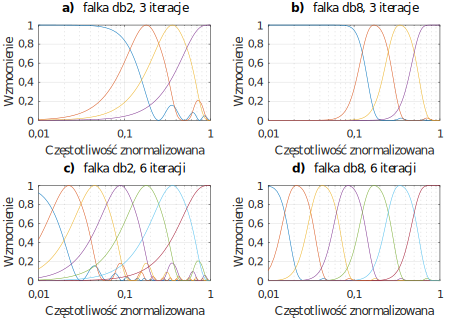
\includegraphics{obrazki/bank_db_demo}
\makecaption{fig:demo_db}{Przykładowe banki filtrów dla rodziny falek \enquote{Daubechies}}
\end{center}
\end{figure}

Przedstawiona na osi pionowej maksymalna wartość wzmocnienia w funkcji częstotliwości sygnału może być w rzeczywistości większa od jedności. W praktyce każdy z fragmentów banku filtrów traktować można jako pasmowo-przepustowy filtr cyfrowy i opisywać za pomocą modelu filtru o skończonej odpowiedzi impulsowej (\enquote{FIR}). Z punktu widzenia pojedynczej wielkości wyjściowej, algorytm transformacji falkowej może być zatem rozumiany jako odpowiednio zaprojektowany filtr, który z sygnału wejściowego przenosi na wyjście wybrane harmoniczne sygnału wejściowego z odpowiednim wzmocnieniem i przesunięciem fazowym. Przedstawione cechy banku filtrów będą bardzo istotne w dalszym etapie pracy w szczególności do określania, w jaki sposób algorytm przenosi błędy opisane w pracy jako dynamiczne. Należy zauważyć, że skoro kolejne filtry w banku odpowiadają kolejnym etapom dekompozycji sygnału, to w większości przypadków właściwości metrologiczne będą jednakowe dla wszystkich wielkości wyjściowych powiązanych z identycznym etapem dekompozycji sygnału, co znacznie upraszcza proces analizy właściwości metrologicznych omawianych algorytmów. Należy jednak mieć na uwadze, że w pewnych przypadkach wypadkowe właściwości toru pomiarowego mogą ulec zmianie, jeżeli wprowadzona zostanie dodatkowa modyfikacja wielkości wejściowych algorytmu transformacji falkowej (np. wprowadzone zostanie okno pomiarowe). Należy w takim przypadku analizować właściwości metrologiczne każdej wielkości wyjściowej z osobna, a nie, jak w klasycznym przypadku, analizować je zbiorczo dla danego etapu dekompozycji.

\begin{figure}[htb!]
\begin{center}
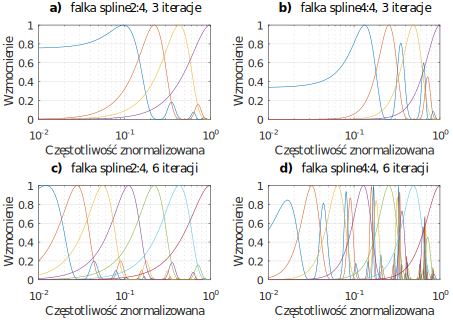
\includegraphics{obrazki/bank_spline_demo}
\makecaption{fig:demo_spline}{Przykładowe banki filtrów dla rodziny falek \enquote{Spline}}
\end{center}
\end{figure}

\section{Macierzowa postać algorytmu}

Ze względu na bardzo dużą liczbę opisanych w literaturze falek~\cite{akujuobi_applications}, ich unikatowe właściwości oraz możliwość zmiany parametrów procesu dekompozycji sygnału, metody analityczne określenia właściwości metrologicznych dla wybranej kombinacji parametrów okazują się czasochłonne i niepraktyczne~\cite{yan_uncertainty, wilczok_uncertainty, peretto_uncertainty, sarrafi_uncertainty}. Opisywane w literaturze falki obejmują między innymi rodziny: \enquote{Daubechies}~\cite{vonesch_dbbasics}, \enquote{Haara}~\cite{stankovic_haar}, \enquote{Coiflet}~\cite{wei_coiflet}, \enquote{Biortogonalne}~\cite{sweldens_bior}, \enquote{Morleta}~\cite{cohen_morlet}, \enquote{Meksykańskiej czapki}~\cite{singh_mexican}, oraz \enquote{Spline}~\cite{averbuch_spline, wang_splinebasics}. Każdą falkę oraz przypisaną do niej funkcję skalującą opisują odpowiednie równania, przy czym nie zawsze są one przedstawiane w postaci jawnej -- w wielu przypadkach rodzina falek opisana jest przez zbiór zależności określających wymagane przez nią założenia, co jeszcze bardziej komplikuje proces analizy tych algorytmów~\cite{rowe_dbmath}. Podczas projektowania toru pomiarowego często istnieje potrzeba zmiany parametrów algorytmu transformacji falkowej, co pociąga za sobą konieczność przeprowadzenia powtórnej analizy jego właściwości metrologicznych. Wszystkie te czynniki sprawiają, że analiza ta jest najczęściej pomijana w pracach opisujących aplikacje omawianych algorytmów. Z opisywanych właściwości algorytmów transformacji falkowej wynika potrzeba przedstawienia uniwersalnej metody umożliwiającej analizę właściwości metrologicznych tych algorytmów. Metoda ta musi być przystępna w aplikacji oraz musi zakładać, że projektant toru pomiarowego nie jest ekspertem w dziedzinie transformacji falkowej, a jedynie jej użytkownikiem. Co więcej, ewentualna zmiana parametrów zastosowanego algorytmu nie może być kłopotliwa z punktu widzenia określenia nowych właściwości metrologicznych analizowanego algorytmu.

Problem skomplikowanej analizy algorytmów transformacji falkowej, podobnie jak w przypadku innych algorytmów przetwarzających ciągi danych, uprościć można przedstawiając analizowany algorytm w postaci macierzowej~\cite{jakubiec_algorithms, jakubiec_system}. Wektor wielkości wyjściowych algorytmu jest w omawianym przypadku równy iloczynowi macierzy transformacji i wektora wielkości wejściowych, co opisano równaniem~\eqref{eq:alg_out_mat}. Przedstawienie algorytmu transformacji falkowej w formie macierzowej umożliwia stworzenie jednolitego i uniwersalnego opisu działania tego algorytmu oraz w znaczącym stopniu ułatwia jego analizę w kolejnych rozdziałach pracy. Zwykle projektant toru pomiarowego nie jest ekspertem w dziedzinie algorytmów transformacji falkowej -- jest on ekspertem w dziedzinie analizowanego zjawiska, a transformacja falkowa jest dla niego jedynie narzędziem, umożliwiającym jego analizę. Stąd, w większości przypadków, osoba ta stosuje gotowe biblioteki zaimplementowane np. dla środowisk \enquote{Matlab}, \enquote{GNU Octave} czy \enquote{PyWavelets}~\cite{lee_pywavelets, misiti_matlabwav}.

W celu identyfikacji wartości współczynników macierzy transformacji należy zastosować metodę opisaną w poprzednim rozdziale pracy lub wyznaczyć te wartości analitycznie, co przedstawiono w dalszej cześć rozdziału. Opisany wcześniej algorytm identyfikacji macierzy transformacji może być wykorzystany w środowiskach, które implementują algorytmy transformacji falkowej, przez co projektant toru pomiarowego z łatwością jest w stanie go zastosować. Ewentualna zmiana parametrów algorytmu transformacji falkowej (zmiana liczby wielkości wejściowych, liczby iteracji procesu dekompozycji, czy wybór innej falki-matki) skutkować będzie jedynie koniecznością ponownej identyfikacji wartości współczynników macierzy transformacji.

Poza opisanym algorytmem identyfikacji współczynników macierzy transformacji, bazującym na istniejącej implementacji omawianego algorytmu, istnieje możliwość wyznaczenia wartości tych współczynników przy użyciu zależności przedstawionych we wcześniejszej części rozdziału, opisującej właściwości algorytmu dyskretnej transformacji falkowej. Proces ten jest jednak skomplikowany i uzależniony od założeń związanych z opisem zastosowanej falki-matki i jej funkcji skalującej. Poniżej przedstawiono przykład wyznaczania wartości macierzy transformacji w przypadku zastosowania falki \enquote{db2} dla dwóch iteracji procesu dekompozycji sygnału oraz ośmiu próbek wejściowych sygnału. Macierz transformacji analizowanego algorytmu składa się zatem z $M = 8$ wierszy, co wynika z liczby wielkości wyjściowych algorytmu oraz $N = 8$ kolumn, co wynika z liczby wielkości wejściowych.

Rodzina falek \enquote{Daubechies} (nazywana w skrócie \enquote{db}) została opisana przez Ingrid Daubechies w 1987 roku. Rodzina ta cechuje się ortogonalnością, natomiast nie wykazuje cech symetrii. Poza założeniami opisanymi w poprzednim podrozdziale, danymi w równaniach~\eqref{eq:dwt_orthogonal_mather} oraz od~\eqref{eq:dwt_orthogonal_father} do~\eqref{eq:dwt_scalemulort}, rodzina ta spełnia dodatkowe założenie odnośnie relacji pomiędzy kolejnymi współczynnikami skalującymi, które opisuje następujące równanie~\cite{vonesch_dbbasics}:
\begin{equation}
\sum _{k=0} ^{N_k-1} \emb{-1}^{k} c_{k} k^{m} = 0 \label{eq:db_musthave},
\end{equation}
gdzie $m$ jest liczbą całkowitą z przedziału $\interval{0}{\frac{N_{k}}{2}-1}$. W przypadku falek \enquote{db} oraz ich pochodnych rząd falki wynosi $\frac{N_{k}}{2}$. Falka \enquote{db2}, będąca falką drugiego rzędu, posiada zatem cztery niezerowe współczynniki skalujące. W literaturze spotkać się można również z oznaczeniem \enquote{D4} dla omawianej falki, gdzie zamiast rzędu falki wskazana jest liczba niezerowych współczynników skalujących. Należy zauważyć, że falka \enquote{Daubechies} rzędu pierwszego jest opisana identycznymi zależnościami, jak falka Hara i posiada identyczne właściwości. Z falek \enquote{Daubechies} wywodzą się kolejne rodziny: \enquote{Symleth} oraz \enquote{Coiflet}, które uzupełniają ją o kolejne cechy -- w szczególności symetrię, istotną podczas przetwarzania i analizy obrazów~\cite{wallen_handbook, akujuobi_applications}.

Jako, że falka \enquote{db2} posiada cztery niezerowe współczynniki skalujące oznaczone jako $c_0$, $c_1$, $c_2$, $c_3$, to zgodnie z równaniem~\eqref{eq:dwt_scalefunrek} oraz równaniem~\eqref{eq:dwt_waveletfunrek}, zapisać można równanie falki-matki i funkcji skalującej w postaci:
\begin{gather}
\phi \emb{t} = c_{0} \phi \emb{2t} + c_{1} \phi \left( 2t - 1 \right) + c_{2} \phi \left( 2t - 2 \right) + c_{3} \phi \left( 2t - 3 \right) \label{eq:db2_scalefunrek}, \\
\psi \emb{t} = c_{3} \phi \emb{2t} - c_{2} \phi \left( 2t - 1 \right) + c_{1} \phi \left( 2t - 2 \right) - c_{0} \phi \left( 2t - 3 \right) \label{eq:db2_waveletfunrek}.
\end{gather}
Uwzględniając założenia przedstawione w poprzedniej części rozdziału oraz te wskazane powyżej, zapisać można układ równań wiążący wszystkie przedstawione zależności:
\begin{equation}
\begin{cases}
	c_{0} + c_{1} + c_{2} + c_{3} = 2                 & $na podstawie właściwości~\eqref{eq:dwt_scalefunsum}$ \\
	c_{0}^{2} + c_{1}^{2} + c_{2}^{2} + c_{3}^{2} = 2 & $na podstawie właściwości~\eqref{eq:dwt_scalemulort}$ \\
	c_{0} - c_{1} + c_{2} - c_{3} = 0                 & $na podstawie~\eqref{eq:db_musthave} dla $ m = 0 \\
	- 1 c_{1} + 2 c_{2} - 3 c_{3} = 0                 & $na podstawie~\eqref{eq:db_musthave} dla $ m = 1
\end{cases}
\label{eq:db2_system},
\end{equation}
oraz wskazać jego rozwiązanie, które determinuje następujące wartości kolejnych współczynników skalujących:
\begin{equation}
c_{0} = \frac{1 + \sqrt{3}}{4}, c_{1} = \frac{3 + \sqrt{3}}{4}, c_{2} = \frac{3 - \sqrt{3}}{4}, c_{3} = \frac{1 - \sqrt{3}}{4} \label{eq:db2_coefs},
\end{equation}
przy czym analogicznie postąpić należy w przypadku wyższych rzędów opisywanej falki.

Zgodnie z założeniami odnośnie długości wektora wielkości wejściowych oraz liczby poziomów dekompozycji zauważyć można, że wektor wielkości wyjściowych zawierać będzie dwie próbki związane z aproksymacją sygnału dla skali $m = 2$, dwie próbki związane z detalami sygnału dla skali $m = 2$ oraz cztery próbki związane z detalami dla skali $m = 1$. Oznaczając wektor wielkości wejściowych jako:
\begin{equation}
\mathbf{x}^{T} =
\begin{bmatrix}
S_{0,0} & S_{0,1} & S_{0,2} & S_{0,3} & S_{0,4} & S_{0,5} & S_{0,6} & S_{0,7}
\end{bmatrix}
\label{eq:db2_invect},
\end{equation}
wektor wielkości wyjściowych można opisać w postaci:
\begin{equation}
\mathbf{X}^{T} =
\begin{bmatrix}
S_{2,0} & S_{2,1} & T_{2,0} & T_{2,1} & T_{1,0} & T_{1,1} & T_{1,2} & T_{1,3}
\end{bmatrix}
\label{eq:db2_outvect},
\end{equation}
a następnie zgodnie z równaniem~\eqref{eq:dwt_aproxrek} oraz~\eqref{eq:dwt_detailrek} opisać można kolejne wymienione w równaniu~\eqref{eq:db2_outvect} wielkości wyjściowe za pomocą zależności:
\begin{gather}
S_{2,0} = \frac{1}{\sqrt{2}} \left( c_{0} S_{1,0} + c_{1} S_{1,1} + c_{2} S_{1,2} + c_{3} S_{1,3} \right) \label{eq:db2_outvect_s_2_0}, \\
S_{2,1} = \frac{1}{\sqrt{2}} \left( c_{0} S_{1,2} + c_{1} S_{1,3} + c_{2} S_{1,4} + c_{3} S_{1,5} \right) \label{eq:db2_outvect_s_2_1}, \\
T_{2,0} = \frac{1}{\sqrt{2}} \left( c_{3} S_{1,0} - c_{2} S_{1,1} + c_{1} S_{1,2} - c_{0} S_{1,3} \right) \label{eq:db2_outvect_t_2_0}, \\
T_{2,1} = \frac{1}{\sqrt{2}} \left( c_{3} S_{1,2} - c_{2} S_{1,3} + c_{1} S_{1,4} - c_{0} S_{1,5} \right) \label{eq:db2_outvect_t_2_1}, \\
T_{1,0} = \frac{1}{\sqrt{2}} \left( c_{3} S_{0,0} - c_{2} S_{0,1} + c_{1} S_{0,2} - c_{0} S_{0,3} \right) \label{eq:db2_outvect_t_1_0}, \\
T_{1,1} = \frac{1}{\sqrt{2}} \left( c_{3} S_{0,2} - c_{2} S_{0,3} + c_{1} S_{0,4} - c_{0} S_{0,5} \right) \label{eq:db2_outvect_t_1_1}, \\
T_{1,2} = \frac{1}{\sqrt{2}} \left( c_{3} S_{0,4} - c_{2} S_{0,5} + c_{1} S_{0,6} - c_{0} S_{0,7} \right) \label{eq:db2_outvect_t_1_2}, \\
T_{1,3} = \frac{1}{\sqrt{2}} \left( c_{3} S_{0,6} - c_{2} S_{0,7} + c_{1} S_{0,0} - c_{0} S_{0,1} \right) \label{eq:db2_outvect_t_1_3},
\end{gather}
gdzie symbol $S_{m,n}$ oznacza aproksymacje, natomiast $T_{m,n}$ detale sygnału dla zadanego numeru skali i numeru przesunięcia w czasie. Po przekształceniu otrzymuje się równania:
\begin{gather}
\begin{split}
S_{2,0} =~
	& \frac{1}{\sqrt{2}} \frac{c_{0}}{\sqrt{2}} \left( c_{0} S_{0,0} + c_{1} S_{0,1} + c_{2} S_{0,2} + c_{3} S_{0,3} \right) + \\
	& \frac{1}{\sqrt{2}} \frac{c_{1}}{\sqrt{2}} \left( c_{0} S_{0,2} + c_{1} S_{0,3} + c_{2} S_{0,4} + c_{3} S_{0,5} \right) + \\
	& \frac{1}{\sqrt{2}} \frac{c_{2}}{\sqrt{2}} \left( c_{0} S_{0,4} + c_{1} S_{0,5} + c_{2} S_{0,6} + c_{3} S_{0,7} \right) + \\
	& \frac{1}{\sqrt{2}} \frac{c_{3}}{\sqrt{2}} \left( c_{0} S_{0,6} + c_{1} S_{0,7} + c_{2} S_{0,0} + c_{3} S_{0,1} \right)
\end{split}
\label{eq:db2_outvect_s_2_0_rek}, \\
\begin{split}
S_{2,1} =~
	& \frac{1}{\sqrt{2}} \frac{c_{0}}{\sqrt{2}} \left( c_{0} S_{0,4} + c_{1} S_{0,5} + c_{2} S_{0,6} + c_{3} S_{0,7} \right) + \\
	& \frac{1}{\sqrt{2}} \frac{c_{1}}{\sqrt{2}} \left( c_{0} S_{0,6} + c_{1} S_{0,7} + c_{2} S_{0,0} + c_{3} S_{0,1} \right) + \\
	& \frac{1}{\sqrt{2}} \frac{c_{2}}{\sqrt{2}} \left( c_{0} S_{0,0} + c_{1} S_{0,1} + c_{2} S_{0,2} + c_{3} S_{0,3} \right) + \\
	& \frac{1}{\sqrt{2}} \frac{c_{3}}{\sqrt{2}} \left( c_{0} S_{0,2} + c_{1} S_{0,3} + c_{2} S_{0,4} + c_{3} S_{0,5} \right)
\end{split}
\label{eq:db2_outvect_s_2_1_rek}, \\
\begin{split}
T_{2,0} =~
	& \frac{1}{\sqrt{2}} \frac{c_{3}}{\sqrt{2}} \left( c_{0} S_{0,0} + c_{1} S_{0,1} + c_{2} S_{0,2} + c_{3} S_{0,3} \right) - \\
	& \frac{1}{\sqrt{2}} \frac{c_{2}}{\sqrt{2}} \left( c_{0} S_{0,2} + c_{1} S_{0,3} + c_{2} S_{0,4} + c_{3} S_{0,5} \right) + \\
	& \frac{1}{\sqrt{2}} \frac{c_{1}}{\sqrt{2}} \left( c_{0} S_{0,4} + c_{1} S_{0,5} + c_{2} S_{0,6} + c_{3} S_{0,7} \right) - \\
	& \frac{1}{\sqrt{2}} \frac{c_{0}}{\sqrt{2}} \left( c_{0} S_{0,6} + c_{1} S_{0,7} + c_{2} S_{0,0} + c_{3} S_{0,1} \right)
\end{split}
\label{eq:db2_outvect_t_2_0_rek}, \\
\begin{split}
T_{2,1} =~
	& \frac{1}{\sqrt{2}} \frac{c_{3}}{\sqrt{2}} \left( c_{0} S_{0,4} + c_{1} S_{0,5} + c_{2} S_{0,6} + c_{3} S_{0,7} \right) - \\
	& \frac{1}{\sqrt{2}} \frac{c_{2}}{\sqrt{2}} \left( c_{0} S_{0,6} + c_{1} S_{0,7} + c_{2} S_{0,0} + c_{3} S_{0,1} \right) + \\
	& \frac{1}{\sqrt{2}} \frac{c_{1}}{\sqrt{2}} \left( c_{0} S_{0,0} + c_{1} S_{0,1} + c_{2} S_{0,2} + c_{3} S_{0,3} \right) - \\
	& \frac{1}{\sqrt{2}} \frac{c_{0}}{\sqrt{2}} \left( c_{0} S_{0,2} + c_{1} S_{0,3} + c_{2} S_{0,4} + c_{3} S_{0,5} \right)
\end{split}
\label{eq:db2_outvect_t_2_1_rek}.
\end{gather}
Grupując odpowiednie wyrazy w zależnościach od~\eqref{eq:db2_outvect_s_2_0_rek} do~\eqref{eq:db2_outvect_t_2_1_rek}, a następnie podstawiając $S_{0,i} = x_{i} = x(i)$, otrzymuje się:
\begin{gather}
\begin{split}
S_{2,0} =~
	& \frac{c_{0}^{2} + c_{2} c_{3}}{2} x_{0} + \frac{c_{0} c_{1} + c_{3}^{2}}{2} x_{1} + \frac{c_{0} c_{2} + c_{0} c_{1}}{2} x_{2} + \frac{c_{0} c_{3} + c_{1}^{2}}{2} x_{3} + \\
	& \frac{c_{1} c_{2} + c_{0} c_{2}}{2} x_{4} + \frac{c_{1} c_{3} + c_{1} c_{2}}{2} x_{5} + \frac{c_2^{2} + c_{0} c_{3}}{2} x_{6} + \frac{c_{2} c_{3} + c_{1} c_{3}}{2} x_7
\end{split}
\label{eq:db2_outvect_s_2_0_full}, \\
\begin{split}
S_{2,1} =~
	& \frac{c_{1} c_{2} + c_{0} c_{2}}{2} x_{0} + \frac{c_{1} c_{3} + c_{1} c_{2}}{2} x_{1} + \frac{c_2^{2} + c_{0} c_{3}}{2} x_{2} + \frac{c_{2} c_{3} + c_{1} c_{3}}{2} x_{3} + \\
	& \frac{c_0^{2} + c_{2} c_{3}}{2} x_{4} + \frac{c_{0} c_{1} + c_3^{2}}{2} x_{5} + \frac{c_{0} c_{2} + c_{0} c_{1}}{2} x_{6} + \frac{c_{0} c_{3} + c_1^{2}}{2} x_7
\end{split}
\label{eq:db2_outvect_s_2_1_full}, \\
\begin{split}
T_{2,0} =~
	& \frac{c_{0} c_{3} - c_{0} c_{2}}{2} x_{0} + \frac{c_{1} c_{3} - c_{0} c_{3}}{2} x_{1} + \frac{c_{2} c_{3} - c_{0} c_{2}}{2} x_{2} + \frac{c_3^{2} - c_{1} c_{2}}{2} x_{3} + \\
	& \frac{c_{0} c_{1} - c_2^{2}}{2} x_{4} + \frac{c_1^{2} - c_{2} c_{3}}{2} x_{5} + \frac{c_{1} c_{2} - c_0^{2}}{2} x_{6} + \frac{c_{1} c_{3} - c_{0} c_{1}}{2} x_7
\end{split}
\label{eq:db2_outvect_t_2_0_full}, \\
\begin{split}
T_{2,1} =~
	& \frac{c_{0} c_{1} - c_2^{2}}{2} x_{0} + \frac{c_1^{2} - c_{2} c_{3}}{2} x_{1} + \frac{c_{1} c_{2} - c_0^{2}}{2} x_{2} + \frac{c_{1} c_{3} - c_{0} c_{1}}{2} x_{3} + \\
	& \frac{c_{0} c_{3} - c_{0} c_{2}}{2} x_{4} + \frac{c_{1} c_{3} - c_{0} c_{3}}{2} x_{5} + \frac{c_{2} c_{3} - c_{0} c_{2}}{2} x_{6} + \frac{c_3^{2} - c_{1} c_{2}}{2} x_7
\end{split}
\label{eq:db2_outvect_t_2_1_full}, \\
T_{1,0} =
	\frac{c_{3}}{\sqrt{2}} x_{0} + \frac{- c_{2}}{\sqrt{2}} x_{1} + \frac{c_{1}}{\sqrt{2}} x_{2} + \frac{- c_{0}}{\sqrt{2}} x_{3} +
	\frac{0}{\sqrt{2}} x_{4} + \frac{0}{\sqrt{2}} x_{5} + \frac{0}{\sqrt{2}} x_{6} + \frac{0}{\sqrt{2}} x_{7}
\label{eq:db2_outvect_t_1_0_full}, \\
T_{1,1} =
	\frac{0}{\sqrt{2}} x_{0} + \frac{0}{\sqrt{2}} x_{1} + \frac{c_{3}}{\sqrt{2}} x_{2} + \frac{- c_{2}}{\sqrt{2}} x_{3} +
	\frac{c_{1}}{\sqrt{2}} x_{4} + \frac{- c_{0}}{\sqrt{2}} x_{5} + \frac{0}{\sqrt{2}} x_{6} + \frac{0}{\sqrt{2}} x_{7}
\label{eq:db2_outvect_t_1_1_full}, \\
T_{1,2} =
	\frac{0}{\sqrt{2}} x_{0} + \frac{0}{\sqrt{2}} x_{1} + \frac{0}{\sqrt{2}} x_{2} + \frac{0}{\sqrt{2}} x_{3} +
	\frac{c_{3}}{\sqrt{2}} x_{4} + \frac{- c_{2}}{\sqrt{2}} x_{5} + \frac{c_{1}}{\sqrt{2}} x_{6} + \frac{- c_{0}}{\sqrt{2}} x_{7}
\label{eq:db2_outvect_t_1_2_full}, \\
T_{1,3} =
	\frac{c_{1}}{\sqrt{2}} x_{0} + \frac{- c_{0}}{\sqrt{2}} x_{1} + \frac{0}{\sqrt{2}} x_{2} + \frac{0}{\sqrt{2}} x_{3} +
	\frac{0}{\sqrt{2}} x_{4} + \frac{0}{\sqrt{2}} x_{5} + \frac{c_{3}}{\sqrt{2}} x_{6} + \frac{- c_{2}}{\sqrt{2}} x_{7}
\label{eq:db2_outvect_t_1_3_full}.
\end{gather}
Następnie, uwzględniając w równaniu~\eqref{eq:alg_out_mat} kolejność elementów wektora wielkości wyjściowych zgodną z założoną w równaniu~\eqref{eq:db2_outvect}, zapisać można:
\begin{gather}
S_{2,0} = a_{0,0} x_{0} + a_{0,1} x_{1} + a_{0,2} x_{2} + a_{0,3} x_{3} + a_{0,4} x_{4} + a_{0,5} x_{5} + a_{0,6} x_{6} + a_{0,7} x_{7} \label{eq:db2_outvect_s_2_0_row}, \\
S_{2,1} = a_{1,0} x_{0} + a_{1,1} x_{1} + a_{1,2} x_{2} + a_{1,3} x_{3} + a_{1,4} x_{4} + a_{1,5} x_{5} + a_{1,6} x_{6} + a_{1,7} x_{7} \label{eq:db2_outvect_s_2_1_row}, \\
T_{2,0} = a_{2,0} x_{0} + a_{2,1} x_{1} + a_{2,2} x_{2} + a_{2,3} x_{3} + a_{2,4} x_{4} + a_{2,5} x_{5} + a_{2,6} x_{6} + a_{2,7} x_{7} \label{eq:db2_outvect_t_2_0_row}, \\
T_{2,1} = a_{3,0} x_{0} + a_{3,1} x_{1} + a_{3,2} x_{2} + a_{3,3} x_{3} + a_{3,4} x_{4} + a_{3,5} x_{5} + a_{3,6} x_{6} + a_{3,7} x_{7} \label{eq:db2_outvect_t_2_1_row}, \\
T_{1,0} = a_{4,0} x_{0} + a_{4,1} x_{1} + a_{4,2} x_{2} + a_{4,3} x_{3} + a_{4,4} x_{4} + a_{4,5} x_{5} + a_{4,6} x_{6} + a_{4,7} x_{7} \label{eq:db2_outvect_t_1_0_row}, \\
T_{1,1} = a_{5,0} x_{0} + a_{5,1} x_{1} + a_{5,2} x_{2} + a_{5,3} x_{3} + a_{5,4} x_{4} + a_{5,5} x_{5} + a_{5,6} x_{6} + a_{5,7} x_{7} \label{eq:db2_outvect_t_1_1_row}, \\
T_{1,2} = a_{6,0} x_{0} + a_{6,1} x_{1} + a_{6,2} x_{2} + a_{6,3} x_{3} + a_{6,4} x_{4} + a_{6,5} x_{5} + a_{6,6} x_{6} + a_{6,7} x_{7} \label{eq:db2_outvect_t_1_2_row}, \\
T_{1,3} = a_{7,0} x_{0} + a_{7,1} x_{1} + a_{7,2} x_{2} + a_{7,3} x_{3} + a_{7,4} x_{4} + a_{7,5} x_{5} + a_{7,6} x_{6} + a_{7,7} x_{7} \label{eq:db2_outvect_t_1_3_row}.
\end{gather}

Powyższe zależności pozwalają wyznaczyć wartości współczynników macierzy transformacji dla analizowanego algorytmu dyskretnej transformacji falkowej. Po podstawieniu wartości zgodnie z zależnością~\eqref{eq:db2_coefs} oraz biorąc pod uwagę równania od~\eqref{eq:db2_outvect_s_2_0_row} do~\eqref{eq:db2_outvect_t_1_3_row} macierz transformacji przyjmuje postać:
\begin{equation}
\mathbf{A} =
\begin{bmatrix}
\frac{5 - \sqrt{3}}{16} & \frac{5 + \sqrt{3}}{16} & \frac{3 + 3 \sqrt{3}}{16} & \frac{5 + 3 \sqrt{3}}{16} & \frac{3 + \sqrt{3}}{16} & \frac{3 - \sqrt{3}}{16} & \frac{5 - 3 \sqrt{3}}{16} & \frac{3 - 3 \sqrt{3}}{16} \\
\frac{3 + \sqrt{3}}{16} & \frac{3 - \sqrt{3}}{16} & \frac{5 - 3 \sqrt{3}}{16} & \frac{3 - 3 \sqrt{3}}{16} & \frac{5 - \sqrt{3}}{16} & \frac{5 + \sqrt{3}}{16} & \frac{3 + 3 \sqrt{3}}{16} & \frac{5 + 3 \sqrt{3}}{16} \\
- \frac{1 + \sqrt{3}}{16} & \frac{1 - \sqrt{3}}{16} & \frac{3 - 3 \sqrt{3}}{16} & - \frac{1 + \sqrt{3}}{16} & - \frac{3 - 5 \sqrt{3}}{16} & \frac{3 + 5 \sqrt{3}}{16} & \frac{1 - \sqrt{3}}{16} & - \frac{3 + 3 \sqrt{3}}{16} \\
- \frac{3 - 5 \sqrt{3}}{16} & \frac{3 + 5 \sqrt{3}}{16} & \frac{1 - \sqrt{3}}{16} & - \frac{3 + 3 \sqrt{3}}{16} & - \frac{1 + \sqrt{3}}{16} & \frac{1 - \sqrt{3}}{16} & \frac{3 - 3 \sqrt{3}}{16} & - \frac{1 + \sqrt{3}}{16} \\
\frac{1 - \sqrt{3}}{4 \sqrt{2}} & - \frac{3 - \sqrt{3}}{4 \sqrt{2}} & \frac{3 + \sqrt{3}}{4 \sqrt{2}} & - \frac{1 + \sqrt{3}}{4 \sqrt{2}} & 0 & 0 & 0 & 0 \\
0 & 0 & \frac{1 - \sqrt{3}}{4 \sqrt{2}} & - \frac{3 - \sqrt{3}}{4 \sqrt{2}} & \frac{3 + \sqrt{3}}{4 \sqrt{2}} & - \frac{1 + \sqrt{3}}{4 \sqrt{2}} & 0 & 0 \\
0 & 0 & 0 & 0 & \frac{1 - \sqrt{3}}{4 \sqrt{2}} & - \frac{3 - \sqrt{3}}{4 \sqrt{2}} & \frac{3 + \sqrt{3}}{4 \sqrt{2}} & - \frac{1 + \sqrt{3}}{4 \sqrt{2}} \\
\frac{3 + \sqrt{3}}{4 \sqrt{2}} & - \frac{1 + \sqrt{3}}{4 \sqrt{2}} & 0 & 0 & 0 & 0 & \frac{1 - \sqrt{3}}{4 \sqrt{2}} & - \frac{3 - \sqrt{3}}{4 \sqrt{2}}
\end{bmatrix}
\label{eq:db2_2_8_matrix}.
\end{equation}
W analogiczny sposób wyznaczyć można wartości elementów macierzy transformacji dla innej liczby wielkości wejściowych algorytmu oraz dowolnej liczby poziomów dekompozycji. W przypadku zastosowania innych rodzin falek należy zastosować odpowiednie dla nich założenia i na ich podstawie wyznaczyć kolejne wielkości niezbędne do określenia wartości elementów identyfikowanej macierzy, przy czym procedura ta przebiega podobnie, jak przedstawiono w powyższym przykładzie.

\section{Przenoszenie błędów przez algorytm}

Jako, że algorytm transformacji falkowej przedstawić można w formie macierzowej, istnieje możliwość analizy jego właściwości metrologicznych zgodnie z metodą przedstawioną w poprzednim rozdziale pracy. Należy zauważyć, że parametry macierzy transformacji wynikające z charakterystyki zastosowanej falki-matki są kluczowym czynnikiem mającym wpływ na związek pomiędzy wariancją błędu analizowanej wielkości wyjściowej, a wariancją błędu wielkości wejściowych~\cite{auth_electronics}. Zgodnie z centralnym twierdzeniem granicznym, bez względu na rozkład błędów losowych wielkości wejściowych algorytmu, kształt rozkładu błędu losowego będzie zbliżony do rozkładu normalnego~\cite{jcgm_guide}. Powyższe założenie jest prawdziwe wtedy, gdy algorytm przetwarza wielokrotnie błędy losowe o tych samych parametrach.

Analizując macierz transformacji przedstawioną w równaniu~\eqref{eq:db2_2_8_matrix} zauważyć można, że jest ona podzielona z punktu widzenia wierszy na kilka charakterystycznych obszarów, przy czym ich liczba zależna jest od liczby iteracji procesu dekompozycji sygnału. Każdy z obszarów odpowiada kolejnemu wyjściu algorytmu Malata, który przedstawiono wcześniej na rysunku~\ref{fig:dwt_decomposition}. W obrębie danego obszaru kolejne wartości współczynników macierzy pozostają niezmienne, przy czym ich pozycje są przesunięte o dwie kolumny w prawo w stosunku do wiersza poprzedniego. Zjawisko to wynika z przesunięcia okna pomiarowego (zmiany parametru przesunięcia falki), natomiast liczba kolumn, o którą przesunięta jest pozycja każdego współczynnika, wynika z przeprowadzenia procesu decymacji (do druga wartość jest odrzucana). Z punktu widzenia analizy metrologicznej zauważyć można, że wielkości wyjściowe związane z tym samym parametrem skali mogą być analizowane równocześnie, gdyż odpowiada im filtr o tych samych parametrach, przez co wartości wielkości opisanych w równaniach~\eqref{eq:alg_trans_stat} oraz~\eqref{eq:alg_trans_rand} będą identyczne~\cite{auth_electronics}.

W przypadku falek z rodziny \enquote{Daubechies}, a także ich pochodnych \enquote{Symleth} oraz \enquote{Coiflets}, niezależnie od liczby poziomów dekompozycji, wartość współczynnika $A_{r,i}$ dla wszystkich wielkości wyjściowych każdorazowo wynosić będzie~\num{1}, natomiast wartość współczynnika $A_{s,i}$ dla aproksymacji sygnału wynosić będzie~\num{2}. Zależności te wynikają bezpośrednio z równań~\eqref{eq:dwt_scalefunsum} oraz~\eqref{eq:db_musthave}~\cite{vonesch_dbbasics, wei_coiflet}. Nie oznacza to jednak, że dalsza analiza może zostać pominięta, a algorytm transformacji falkowej nie ma wpływu na przenoszone błędy wielkości wejściowych, ponieważ wciąż istnieje potrzeba analizy pozostałych rodzajów błędów. Ze względu na fakt, że tylko jedna grupa wielkości wyjściowych, związana z aproksymacją sygnału, stanowić będzie filtr dolno-przepustowy, dla pozostałych grup wielkości wyjściowych wartość współczynnika $A_{s,i}$ będzie zwykle zerowa. Wynika to z faktu, że błędy statyczne stanowią składową stałą sygnału, a zatem nie będą przenoszone przez filtry inne, niż dolno-przepustowe.

\section{Błędy własne algorytmu}

Analizując przykładową macierz transformacji przedstawioną w równaniu~\eqref{eq:db2_2_8_matrix}, której wartości wyznaczono we wcześniejszej części rozdziału, zauważyć można, że wszystkie niezerowe wartości elementów tej macierzy są niewymierne. Niewymierność ta jest pierwszym powodem powstawania błędu własnego zaokrągleń, którym obarczone będą wyznaczane numerycznie wielkości wyjściowe algorytmu dyskretnej transformacji falkowej. Kolejnym źródłem błędów będą zaokrąglenia wynikające z ograniczonej precyzji liczb, przeprowadzane podczas wykonywania operacji mnożenia i dodawania. Błędy te, zgodnie ze wcześniej wprowadzonym podziałem, zaliczyć można do błędów losowych ponieważ nie ma możliwości deterministycznego opisu przebiegu sygnału tych błędów, a dodatkowo ich realizacje będą zmienne w obrębie okna pomiarowego.

Zakładając, że analizowana $j$-ta wielkość wyjściowa algorytmu obarczona jest jedynie błędem własnym, który wynika z omówionych w poprzednim akapicie zjawisk, sygnał $e_{X,z}(j)$ związany z tym błędem zdefiniować można w postaci:
\begin{equation}
e_{X,z} \emb{j} = \tilde{X} \emb{j} - \dot{X} \emb{j} \label{eq:fwt_outerr_self}.
\end{equation}
Należy zauważyć, że zależność~\eqref{eq:fwt_outerr_self} jest prawdziwa tylko wtedy, gdy wielkości wejściowe $x(i)$ algorytmu nie są obarczone żadnymi błędami, tj. dla $\tilde{x}(i) = \dot{x}(i)$. Dodatkowo zakłada się, że w przypadku algorytmu idealnego sygnały błędu własnego $e_{X,z}(j)$ nie występują, a zatem dla takiego algorytmu zachodzi $e_{X,z}(j) = 0$.

Parametry rozkładu sygnałów błędów własnych kolejnych wielkości wyjściowych algorytmu wyznaczyć można eksperymentalnie, stosując metodę Monte-Carlo~\cite{jcgm_montecarlo}. Należy w tym celu wielokrotnie podawać na wejście algorytmu wektor wielkości wejściowych, którego wartości kolejnych elementów będą liczbami losowymi. Schemat blokowy pojedynczej iteracji omawianego eksperymentu przedstawia rysunek~\ref{fig:schemat_dwt_ew}, przy czym symbolem $e_{X,z}(j)$ oznaczono sygnał związany z błędami własnymi zaokrągleń algorytmu dla $j$-tej wielkości wyjściowej, natomiast symbolem $x(i)$ kolejne elementy wektora wielkości wejściowych. Parametry rozkładu realizacji wielkości $x(i)$ powinny być zbliżone do rzeczywistych parametrów realizacji wielkości wejściowych algorytmu dla analizowanego toru pomiarowego.

\begin{figure}[htb!]
\begin{center}
\includegraphics{obrazki/schemat_dwt_ew}
\makecaption{fig:schemat_dwt_ew}{Schemat blokowy procedury wyznaczania pojedynczej realizacji sygnału błędu własnego, która przeprowadzana jest w celu określenia parametrów sygnałów błędów własnych analizowanego algorytmu dyskretnej transformacji falkowej}
\end{center}
\end{figure}

W dalszej części podrozdziału zakłada się, że analizowany algorytm przetwarza wielkości wejściowe $x(i)$ o wartościach realizacji z zakresu $\interval{-1}{1}$ i jednakowym prawdopodobieństwie uzyskania każdej z wartości, a dodatkowo wielkości te nie są obarczone żadnym błędem. Zgodnie z równaniem~\eqref{eq:fwt_outerr_self}, błąd własny algorytmu jest zatem równy różnicy pomiędzy wartością $\tilde{X}(j)$ wyznaczoną przez rzeczywisty, a wartością $\dot{X}(j)$ wyznaczoną przez idealny algorytm. Zakłada się, że w przypadku algorytmu rzeczywistego wartości realizacji wielkości wyjściowych wyznaczane są numerycznie na podstawie równania~\eqref{eq:alg_out_mat} dla współczynników macierzy transformacji zidentyfikowanych zgodnie z omówioną wcześniej metodologią, natomiast w przypadku algorytmu idealnego wartości te wyznaczane są analitycznie na podstawie równań~\eqref{eq:dwt_aproxrek} oraz~\eqref{eq:dwt_detailrek} odpowiednich dla stosowanej falki-matki. Przyjmuje się liczbę powtórzeń wyznaczania wartości realizacji sygnału błędu własnego równą~\num{100000}.

Przeprowadzenie omawianego eksperymentu jest w rzeczywistości niemożliwe, ponieważ nie jest możliwe analityczne wyznaczenie wartości wielkości wyjściowych algorytmu dla zadanej liczby powtórzeń eksperymentu. Numeryczna realizacja eksperymentu powoduje, że wszystkie operacje związane z jego przeprowadzeniem również są obarczone błędami numerycznymi~\cite{benz_floats}. Przyjmuje się zatem za wartości idealne $\dot{X}(j)$ wartości wyznaczone zgodnie z równaniem~\eqref{eq:alg_out_mat} przy użyciu liczb rzeczywistych o długości słowa równej~\qty{128}{\bitOw}. Parametry rozkładu błędów własnych algorytmu wyznaczono dla słów o długości~\qty{32}{\bitOw} oraz~\qty{16}{\bitOw}, ponieważ te we współczesnych mikrokontrolerach stosowane są najczęściej~\cite{cortex_dsp, kim_compilers}. Do przeprowadzenia eksperymentu zastosowano program komputerowy przetłumaczony na kod maszynowy kompilatorem \enquote{GNU GCC}~\cite{gcc_manual}. Wybór wskazanego kompilatora podyktowany był faktem, że jest on również stosowany do generowania kodu maszynowego dla mikrokontrolerów rodzin \enquote{ARM} oraz \enquote{AVR}~\cite{kim_compilers, gcc_manual}.

Poniżej, w tabelach od~\ref{tab:varnum_db2_2_f16} do~\ref{tab:varnum_spline4_4_5_f32}, zamieszczono wyniki eksperymentu dla wybranych kombinacji parametrów algorytmu dyskretnej transformacji falkowej. Tabele~\ref{tab:varnum_db2_2_f16} oraz~\ref{tab:varnum_db2_2_f32} zawierają wyniki dla wyznaczonej we wcześniejszej cześć rozdziału, przykładowej macierzy transformacji opisanej równaniem~\eqref{eq:db2_2_8_matrix} oraz uwzględniają zmianę zakresu wartości wielkości wejściowych algorytmu. Rysunek~\ref{fig:dwt_rerror_coif5} przedstawia zależność wartości wariancji sygnału błędów własnych algorytmu od liczby wielkości wejściowych dla wybranych parametrów falki \enquote{coif5} oraz liczby iteracji procesu dekompozycji sygnału, przy czym na omawianym rysunku wskazano wartość dla ostatniej skali detali sygnału. Rysunek~\ref{fig:dwt_rhist_coif5} przedstawia histogramy dla wybranych parametrów eksperymentu przy zastosowaniu falki \enquote{coif5}. Ze względu na fakt, że dla każdego poziomu dekompozycji wartości współczynników macierzy transformacji są jedynie przesunięte względem poprzedniego wiersza o dwie kolumny, co wynika z przesunięcia okna pomiarowego na kolejną pozycję, można przyjąć że wartość wariancji sygnału błędu zaokrągleń jest stała dla tego samego numeru skali, przy czym opisywaną właściwość zaobserwować można analizując wartości zestawione w tabelach~\ref{tab:varnum_db2_2_f16} oraz~\ref{tab:varnum_db2_2_f32}.

\begin{figure}[htb!]
\begin{center}
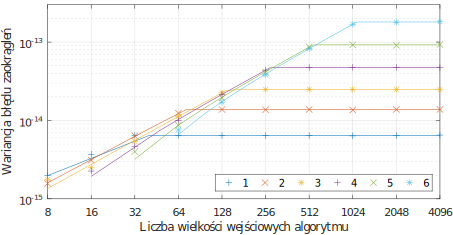
\includegraphics{obrazki/dwt_rerror_coif5}
\makecaption{fig:dwt_rerror_coif5}{Zależność wartości wariancji sygnału błędu własnego zaokrągleń od liczby iteracji procesu dekompozycji sygnału oraz liczby wielkości wejściowych dla falki \enquote{coif5} przy stosowaniu liczb zmiennoprzecinkowych o długości słowa~\qty{32}{\bitOw} dla ostatniej skali detali sygnału}
\end{center}
\end{figure}

Na podstawie rysunku~\ref{fig:dwt_rerror_coif5} zauważyć można liniowy wzrost wartości wariancji sygnału błędu zaokrągleń w funkcji liczby wielkości wejściowych, przy czym wzrost ten ustaje, gdy przestaje zwiększać się liczba operacji arytmetycznych, tj. dla takiej liczby wielkości wejściowych, która jest równa liczbie niezerowych współczynników macierzy transformacji dla analizowanego poziomu dekompozycji sygnału. W przypadku tej samej liczby wielkości wejściowych, wartość wariancji sygnału błędu zaokrągleń rośnie wraz ze wzrostem liczby iteracji procesu dekompozycji sygnału, ponieważ liczba operacji arytmetycznych wzrasta dla wyższych numerów skali, co zauważyć mozna na przykładzie równań~\eqref{eq:db2_outvect_t_1_0} oraz~\eqref{eq:db2_outvect_t_2_0_rek}. Wartość wariancji błędu zaokrągleń związana jest zatem bezpośrednio z liczbą przeprowadzanych operacji arytmetycznych i zależy od liczby współczynników skalujących oraz liczby wielkości wejściowych algorytmu.

Analizując przedstawione na rysunku~\ref{fig:dwt_rhist_coif5} histogramy realizacji sygnału błędu własnego zaokrągleń dla falki \enquote{coif5} zauważyć można, że kształt rozkładu realizacji tego sygnału jest zbliżony do kształtu rozkładu normalnego, natomiast dla poziomu ufności $\alpha = \qty{95}{\percent}$ współczynnik rozszerzenia wynosi około~\num{2.16}. Wobec powyższego, przyjęcie założenia, w którym model sygnału błędu własnego opisywany będzie rozkładem normalnym, nie jest właściwe. Aby możliwe było oszacowanie wartości współczynników koherencji zgodnie z równaniem~\eqref{eq:unc_coher}, konieczne jest wyznaczenie wartości współczynników kształtu, analogicznie jak miało to miejsce w poprzednim rozdziale. Zgodnie z równaniem~\eqref{eq:unc_shapertwo}, stosując metodę Monte-Carlo, oszacowano wartości współczynników kształtu dla sygnału błędu własnego oraz sygnałów błędów o typowych kształtach funkcji gęstości prawdopodobieństwa, a uzyskane wyniki zestawiono w tabeli~\ref{tab:unc_shapedwt}. Z uwagi na fakt, że uzyskane rozkłady sygnałów błędów własnych cechowały się bardzo zbliżonym kształtem, przedstawione wyniki stanowią uśrednione wartości dla wszystkich przeprowadzonych wcześniej eksperymentów. W dalszej cześć pracy przyjmuje się, że współczynnik kształtu oznaczony symbolem $c_{z}$ odpowiadać będzie sygnałowi błędu zaokrągleń oraz że $c_{z} = \num{2.16}$.

\begin{table}[htb!]
\begin{center}
\makecaption{tab:unc_shapedwt}{Wartości współczynników kształtu dla typowych kształtów rozkładów oraz rozkładu sygnału błędu zaokrągleń algorytmu transformacji falkowej, gdzie kolejne symbole oznaczają rozkład: (n)~normalny, (u)~jednostajny, (t)~trójkątny, (d)~dwumodalny, (r)~zaokrągleń}
\begin{tabular}[c]{| c *{5}{| S[table-format = +1.3] } |} \hline
$s_{r,*}$ & \textbf{$n$} & \textbf{$u$} & \textbf{$t$} & \textbf{$d$} & \textbf{$r$} \\ \hline
$r$       & -0.009       & 0.066        & -0.010       & 0.197        & 0.027        \\ \hline
\end{tabular}
\end{center}
\end{table}

\begin{figure}[htb!]
\begin{center}
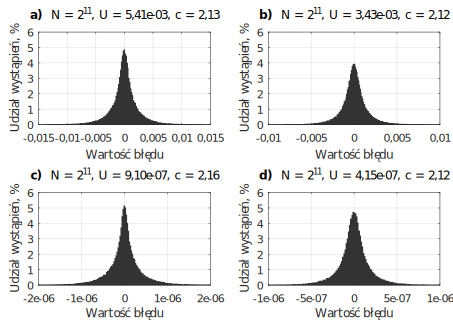
\includegraphics{obrazki/hist_numerr_coif5}
\makecaption{fig:dwt_rhist_coif5}{Histogramy realizacji sygnału błędu własnego zaokrągleń dla falki \enquote{coif5} przy sześciu iteracjach procesu dekompozycji, dla $N$ wielkości wejściowych, przy długości słowa równej \textbf{a)},~\textbf{b)}~\qty{16}{\bitOw}, \textbf{c)},~\textbf{d)}~\qty{32}{\bitOw}, przy czym niepewność rozszerzoną wyznaczono dla poziomu ufności równego \qty{95}{\percent}}
\end{center}
\end{figure}

Stosowanie liczb zmiennoprzecinkowych o długości słowa~\qty{16}{\bitOw} pozwala zmniejszyć czas obliczeń oraz rozmiar wymaganej pamięci operacyjnej w stosunku do analogicznego przypadku, wykorzystującego liczby o długości słowa~\qty{32}{\bitOw}~\cite{reay_dsp, gcc_manual}. Wariant ten wprowadza jednak znacznie większe wartości realizacji sygnałów błędów związanych z zaokrągleniami oraz większe wartości wariancji tych sygnałów ze względu na ograniczoną precyzję stosowanego zapisu liczb, co zauważyć można porównując dane zawarte w tabelach~\ref{tab:varnum_db2_2_f16} oraz~\ref{tab:varnum_db2_2_f32} dotyczące falki \enquote{db2}. W praktyce należy zatem tak dobrać długość słowa stosowanych liczb zmiennoprzecinkowych, aby wartość wariancji sygnału błędu zaokrągleń była możliwie mała w stosunku do wartości wariancji pozostałych sygnałów błędów na wyjściu algorytmu. Jeżeli przedstawione założenie zostanie spełnione, to sygnał błędu własnego algorytmu transformacji falkowej będzie mógł zostać pominięty podczas analizy właściwości toru pomiarowego~\cite{jcgm_guide}.

\begin{table}[htb!]
\begin{center}
\makecaption{tab:varnum_db2_2_f16}{Zestawienie uzyskanych symulacyjnie wartości wariancji sygnału błędu zaokrągleń kolejnych wielkości wyjściowych algorytmu dyskretnej transformacji falkowej dla falki \enquote{db2} przy dwóch iteracjach procesu dekompozycji, dla liczb o długości~\qty{16}{\bitOw}, w zależności od zakresu możliwych wartości realizacji wielkości wejściowych}
\begin{tabular}[c]{| c *{6}{|S[table-format = 1.2e+1, mode = math]} |} \hline
\multirow{2}{*}{$X$} & \multicolumn{6}{ c |}{\textbf{Zakres wartości realizacji wielkości wejściowych algorytmu}} \\ \cline{2-7}
& $\interval{-1}{1}$ & $\interval{-2}{2}$ & $\interval{-3}{3}$ & $\interval{0}{2}$ & $\interval{0}{4}$ & $\interval{3}{9}$ \\ \hline
$S_{2,0}$ & 1.03e-7 & 4.12e-7 & 9.74e-7 & 7.08e-7 & 2.83e-6 & 2.16e-5 \\ \hline
$S_{2,1}$ & 1.11e-7 & 4.43e-7 & 1.01e-6 & 9.55e-7 & 3.82e-6 & 2.75e-5 \\ \hline
$T_{2,0}$ & 1.31e-7 & 5.24e-7 & 1.21e-6 & 2.87e-7 & 1.15e-6 & 7.06e-6 \\ \hline
$T_{2,1}$ & 1.07e-7 & 4.29e-7 & 9.73e-7 & 3.36e-7 & 1.34e-6 & 9.30e-6 \\ \hline
$T_{1,0}$ & 7.09e-8 & 2.85e-7 & 6.99e-7 & 1.65e-7 & 3.56e-7 & 4.29e-6 \\ \hline
$T_{1,1}$ & 5.83e-8 & 2.33e-7 & 5.87e-7 & 1.49e-7 & 5.95e-7 & 4.05e-6 \\ \hline
$T_{1,2}$ & 5.84e-8 & 2.34e-7 & 5.85e-7 & 1.49e-7 & 5.97e-7 & 4.05e-6 \\ \hline
$T_{1,3}$ & 5.53e-8 & 2.21e-7 & 5.41e-7 & 1.78e-7 & 7.08e-7 & 5.26e-6 \\ \hline
\end{tabular}
\end{center}
\end{table}

\begin{table}[htb!]
\begin{center}
\makecaption{tab:varnum_db2_2_f32}{Zestawienie uzyskanych symulacyjnie wartości wariancji sygnału błędu zaokrągleń kolejnych wielkości wyjściowych algorytmu dyskretnej transformacji falkowej dla falki \enquote{db2} przy dwóch iteracjach procesu dekompozycji, dla liczb o długości~\qty{32}{\bitOw}, w zależności od zakresu możliwych wartości realizacji wielkości wejściowych}
\begin{tabular}[c]{| c *{6}{|S[table-format = 1.2e+2, mode = math]} |} \hline
\multirow{2}{*}{$X$} & \multicolumn{6}{ c |}{\textbf{Zakres wartości realizacji wielkości wejściowych algorytmu}} \\ \cline{2-7}
& $\interval{-1}{1}$ & $\interval{-2}{2}$ & $\interval{-3}{3}$ & $\interval{0}{2}$ & $\interval{0}{4}$ & $\interval{3}{9}$ \\ \hline
$S_{2,0}$ & 1.40e-15 & 5.57e-15 & 1.30e-14 & 9.29e-15 & 3.71e-14 & 2.78e-13 \\ \hline
$S_{2,1}$ & 1.40e-15 & 5.61e-15 & 1.29e-14 & 1.25e-14 & 5.00e-14 & 3.54e-13 \\ \hline
$T_{2,0}$ & 1.71e-15 & 6.83e-15 & 1.58e-14 & 3.33e-15 & 1.33e-14 & 7.78e-14 \\ \hline
$T_{2,1}$ & 1.39e-15 & 5.56e-15 & 1.29e-14 & 4.27e-15 & 1.71e-14 & 1.16e-13 \\ \hline
$T_{1,0}$ & 8.28e-16 & 3.54e-15 & 8.38e-15 & 1.70e-15 & 6.84e-15 & 4.25e-14 \\ \hline
$T_{1,1}$ & 6.82e-16 & 2.72e-15 & 6.67e-15 & 1.46e-15 & 5.84e-15 & 4.02e-14 \\ \hline
$T_{1,2}$ & 6.82e-16 & 2.72e-15 & 6.66e-15 & 1.47e-15 & 5.86e-15 & 4.02e-14 \\ \hline
$T_{1,3}$ & 6.68e-16 & 2.67e-15 & 6.48e-15 & 2.02e-15 & 8.10e-15 & 6.15e-14 \\ \hline
\end{tabular}
\end{center}
\end{table}

Jako, że zakres możliwych wartości realizacji wielkości wejściowych algorytmu transformacji falkowej również wpływa na wprowadzane błędy zaokrągleń, należy brać ten czynnik pod uwagę podczas analizy projektowanego toru pomiarowego. Podobna zależność występuje również dla kształtu rozkładu realizacji omawianego sygnału. Należy zatem tak dobrać warunki eksperymentu mającego na celu identyfikacje parametrów sygnału błędu własnego, aby w jak największym stopniu były one zbieżne z warunkami rzeczywistymi. Analizując wyniki eksperymentu zauważyć można, że wraz ze wzrostem zakresu wartości wielkości wejściowych wartość wariancji sygnału błędu zaokrągleń wzrasta. Zależność ta wynika bezpośrednio z właściwości stosowanej metody zapisu liczb zmiennoprzecinkowych i została szerzej opisana w publikacji~\cite{benz_floats}.

\begin{table}[htb!]
\begin{center}
\makecaption{tab:varnum_db2_5_f16}{Zestawienie uzyskanych symulacyjnie wartości wariancji sygnału błędu zaokrągleń kolejnych grup wielkości wyjściowych algorytmu dyskretnej transformacji falkowej dla falki \enquote{db2} przy pięciu iteracjach procesu dekompozycji, dla liczb o długości~\qty{16}{\bitOw}, w zależności od liczby wielkości wejściowych algorytmu}
\begin{tabular}[c]{| c *{6}{|S[table-format = 1.2e+1, mode = math]} |} \hline
\multirow{2}{*}{$N$} & \multicolumn{6}{ c |}{\textbf{Skala wielkości wyjściowych algorytmu}} \\ \cline{2-7}
& \text{$S_5$} & \text{$T_5$} & \text{$T_4$} & \text{$T_3$} & \text{$T_2$} & \text{$T_1$} \\ \hline
\textbf{64}   & 4.91e-7 & 5.31e-7 & 3.94e-7 & 2.09e-7 & 1.23e-7 & 5.86e-8 \\ \hline
\textbf{128}  & 7.51e-7 & 7.08e-7 & 3.87e-7 & 2.07e-7 & 1.22e-7 & 5.85e-8 \\ \hline
\textbf{256}  & 8.59e-7 & 6.99e-7 & 3.85e-7 & 2.05e-7 & 1.21e-7 & 5.84e-8 \\ \hline
\textbf{512}  & 9.19e-7 & 6.89e-7 & 3.81e-7 & 2.04e-7 & 1.21e-7 & 5.84e-8 \\ \hline
\textbf{1024} & 9.47e-7 & 6.85e-7 & 3.80e-7 & 2.04e-7 & 1.21e-7 & 5.84e-8 \\ \hline
\textbf{2048} & 9.58e-7 & 6.84e-7 & 3.80e-7 & 2.04e-7 & 1.21e-7 & 5.84e-8 \\ \hline
\textbf{4096} & 9.66e-7 & 6.83e-7 & 3.80e-7 & 2.04e-7 & 1.21e-7 & 5.84e-8 \\ \hline
\end{tabular}
\end{center}
\end{table}

\begin{table}[htb!]
\begin{center}
\makecaption{tab:varnum_db2_5_f32}{Zestawienie uzyskanych symulacyjnie wartości wariancji sygnału błędu zaokrągleń kolejnych grup wielkości wyjściowych algorytmu dyskretnej transformacji falkowej dla falki \enquote{db2} przy pięciu iteracjach procesu dekompozycji, dla liczb o długości~\qty{32}{\bitOw}, w zależności od liczby wielkości wejściowych algorytmu}
\begin{tabular}[c]{| c *{6}{|S[table-format = 1.2e+2, mode = math]} |} \hline
\multirow{2}{*}{$N$} & \multicolumn{6}{ c |}{\textbf{Skala wielkości wyjściowych algorytmu}} \\ \cline{2-7}
& \text{$S_5$} & \text{$T_5$} & \text{$T_4$} & \text{$T_3$} & \text{$T_2$} & \text{$T_1$} \\ \hline
\textbf{64}   & 6.83e-15 & 7.93e-15 & 5.42e-15 & 2.86e-15 & 1.62e-15 & 7.12e-16 \\ \hline
\textbf{128}  & 1.15e-14 & 1.02e-14 & 5.39e-15 & 2.79e-15 & 1.58e-15 & 6.98e-16 \\ \hline
\textbf{256}  & 1.34e-14 & 1.03e-14 & 5.30e-15 & 2.76e-15 & 1.56e-15 & 6.90e-16 \\ \hline
\textbf{512}  & 1.44e-14 & 1.03e-14 & 5.25e-15 & 2.73e-15 & 1.55e-15 & 6.85e-16 \\ \hline
\textbf{1024} & 1.49e-14 & 1.03e-14 & 5.23e-15 & 2.72e-15 & 1.55e-15 & 6.84e-16 \\ \hline
\textbf{2048} & 1.51e-14 & 1.03e-14 & 5.22e-15 & 2.72e-15 & 1.55e-15 & 6.84e-16 \\ \hline
\textbf{4096} & 1.52e-14 & 1.03e-14 & 5.22e-15 & 2.72e-15 & 1.55e-15 & 6.84e-16 \\ \hline
\end{tabular}
\end{center}
\end{table}

\begin{table}[htb!]
\begin{center}
\makecaption{tab:varnum_spline4_4_5_f16}{Zestawienie uzyskanych symulacyjnie wartości wariancji sygnału błędu zaokrągleń kolejnych grup wielkości wyjściowych algorytmu dyskretnej transformacji falkowej dla falki \enquote{spline2:4} przy pięciu iteracjach procesu dekompozycji, dla liczb o długości~\qty{16}{\bitOw}, w zależności od liczby wielkości wejściowych algorytmu}
\begin{tabular}[c]{| c *{6}{|S[table-format = 1.2e+1, mode = math]} |} \hline
\multirow{2}{*}{$N$} & \multicolumn{6}{ c |}{\textbf{Skala wielkości wyjściowych algorytmu}} \\ \cline{2-7}
& \text{$S_5$} & \text{$T_5$} & \text{$T_4$} & \text{$T_3$} & \text{$T_2$} & \text{$T_1$} \\ \hline
\textbf{64}   & 1.07e-6 & 1.02e-6 & 8.94e-7 & 5.05e-7 & 1.83e-7 & 4.76e-8 \\ \hline
\textbf{128}  & 1.75e-6 & 1.59e-6 & 9.22e-7 & 4.96e-7 & 1.80e-7 & 4.64e-8 \\ \hline
\textbf{256}  & 2.61e-6 & 1.67e-6 & 9.11e-7 & 4.91e-7 & 1.77e-7 & 4.58e-8 \\ \hline
\textbf{512}  & 2.60e-6 & 1.69e-6 & 9.05e-7 & 4.89e-7 & 1.76e-7 & 4.55e-8 \\ \hline
\textbf{1024} & 2.58e-6 & 1.71e-6 & 9.02e-7 & 4.88e-7 & 1.75e-7 & 4.53e-8 \\ \hline
\textbf{2048} & 2.58e-6 & 1.71e-6 & 9.00e-7 & 4.87e-7 & 1.75e-7 & 4.53e-8 \\ \hline
\textbf{4096} & 2.58e-6 & 1.72e-6 & 9.00e-7 & 4.87e-7 & 1.75e-7 & 4.53e-8 \\ \hline
\end{tabular}
\end{center}
\end{table}

\begin{table}[htb!]
\begin{center}
\makecaption{tab:varnum_spline4_4_5_f32}{Zestawienie uzyskanych symulacyjnie wartości wariancji sygnału błędu zaokrągleń kolejnych grup wielkości wyjściowych algorytmu dyskretnej transformacji falkowej dla falki \enquote{spline2:4} przy pięciu iteracjach procesu dekompozycji, dla liczb o długości~\qty{32}{\bitOw}, w zależności od liczby wielkości wejściowych algorytmu}
\begin{tabular}[c]{| c *{6}{|S[table-format = 1.2e+2, mode = math]} |} \hline
\multirow{2}{*}{$N$} & \multicolumn{6}{ c |}{\textbf{Skala wielkości wyjściowych algorytmu}} \\ \cline{2-7}
& \text{$S_5$} & \text{$T_5$} & \text{$T_4$} & \text{$T_3$} & \text{$T_2$} & \text{$T_1$} \\ \hline
\textbf{64}   & 1.51e-14 & 1.44e-14 & 1.26e-14 & 6.54e-15 & 2.33e-15 & 5.44e-16 \\ \hline
\textbf{128}  & 2.52e-14 & 2.37e-14 & 1.45e-14 & 6.50e-15 & 2.27e-15 & 5.29e-16 \\ \hline
\textbf{256}  & 4.72e-14 & 2.91e-14 & 1.45e-14 & 6.40e-15 & 2.24e-15 & 5.22e-16 \\ \hline
\textbf{512}  & 4.72e-14 & 2.98e-14 & 1.44e-14 & 6.36e-15 & 2.23e-15 & 5.17e-16 \\ \hline
\textbf{1024} & 4.71e-14 & 3.01e-14 & 1.43e-14 & 6.35e-15 & 2.22e-15 & 5.16e-16 \\ \hline
\textbf{2048} & 4.72e-14 & 3.03e-14 & 1.43e-14 & 6.35e-15 & 2.22e-15 & 5.16e-16 \\ \hline
\textbf{4096} & 4.72e-14 & 3.04e-14 & 1.43e-14 & 6.35e-15 & 2.22e-15 & 5.16e-16 \\ \hline
\end{tabular}
\end{center}
\end{table}

\section{Implementacja okna pomiarowego}

Identycznie, jak w przypadku innych algorytmów przetwarzających ciągi wielkości wejściowych, dla algorytmu transformacji falkowej stosować można wybrane okno pomiarowe. Wprowadzenie okna pomiarowego, którego funkcję oznaczono symbolem $w(n)$, można przedstawić za pomocą modyfikacji równania~\eqref{eq:alg_out_single}:
\begin{equation}
X \emb{i} = a_{i, 0} w \emb{0} x \emb{0} + a_{i, 1} w \emb{1} x \emb{1} + \hdots + a_{i, N-1} w \emb{N-1} x \emb{N-1} \label{eq:wt_singlewindow}.
\end{equation}
Na podstawie przedstawionego równania zauważyć można, że wprowadzenie okna pomiarowego opisać można również za pomocą modyfikacji współczynników macierzy transformacji algorytmu zgodnie z zależnością opisaną równaniem:
\begin{equation}
a'_{i,j} = w \emb{j} a_{i,j} \label{eq:wt_windowmod},
\end{equation}
gdzie $a'_{i,j}$ stanowi nową wartość współczynnika macierzy transformacji algorytmu. Użyta funkcja $w(n)$ powinna być opisana dla wartości $n$ w przedziale $\interval{0}{N-1}$. Należy zaznaczyć, że stosowanie okna pomiarowego spowoduje zmianę transmitancji związanych z kolejnymi wielkościami wyjściowymi algorytmu, a zatem będzie miało wpływ na widmo sygnałów wielkości wyjściowych.

Wybrane okna pomiarowe opisane w literaturze~\cite{oppenheim_dsp, oppenheim_sns, proakis_dsp} to okna: trójkątne~\eqref{eq:wnd_triang}, sinusoidalne~\eqref{eq:wnd_sine}, Gaussa~\eqref{eq:wnd_gauss}, Hamminga~\eqref{eq:wnd_hamming}, Hanna~\eqref{eq:wnd_hann} oraz Welcha~\eqref{eq:wnd_welch}, które opisać można kolejno w postaci:
\begin{gather}
w_{tr} \emb{n} = 1 - \left| \frac{n - \frac{N-1}{2}}{\frac{N}{2}} \right| \label{eq:wnd_triang}, \\
w_{sn} \emb{n} = \sin \left( \frac{\pi n}{N} \right) \label{eq:wnd_sine}, \\
w_{ga} \emb{n} = \exp \left(-\frac{1}{2} \left( \frac{n - \frac{N-1}{2}}{\sigma \frac{\emb{N-1}}{2}} \right)^{2} \right) \label{eq:wnd_gauss}, \\
w_{hm} \emb{n} = \num{0.5384} - \num{0.4616} \cos \left( \frac{2 \pi n}{N} \right) \label{eq:wnd_hamming}, \\
w_{hn} \emb{n} = \num{0.5} \left(1 - \cos \left( \frac{2 \pi n}{N} \right) \right) \label{eq:wnd_hann}, \\
w_{wh} \emb{n} = 1 - \left( \frac{n - \frac{N}{2}}{\frac{N}{2}} \right)^{2} \label{eq:wnd_welch}.
\end{gather}
W dalszej części pracy stosuje się okno prostokątne, w którym $w(n) = 1$, o ile nie został zaznaczony fakt stosowania innego okna pomiarowego.

Implementacja okna pomiarowego, z punktu widzenia przedstawionych w pracy założeń, mogłaby również zostać opisana jako zastosowanie dodatkowego algorytmu. Algorytm ten przetwarzałby $N$ wielkości wejściowych na $M$ wielkości wyjściowych, gdzie $N = M$. Macierz transformacji omawianego algorytmu byłaby macierzą diagonalną, przy czym wartości kolejnych współczynników odpowiadałyby wyznaczonym wagom dla $i$-tej wielkości okna. Z praktycznego punktu widzenia zaproponowana metoda modyfikacji wartości współczynników transformacji algorytmu transformacji falkowej wydaje się jednak bardziej korzystna. Na tej samej zasadzie istnieje możliwość implementacji innych modyfikacji, np. wprowadzenia dodatkowego filtru. Jako, że algorytm dyskretnej transformacji sam w sobie implementuje dla kolejnych wielkości wyjściowych podział tych wielkości na odpowiadające im okna pomiarowe, stosowanie dodatkowego okna pomiarowego nie jest tak popularne, jak w przypadku innych algorytmów (np. algorytmu \enquote{DFT}). Zagadnienie to nie zostało zatem poruszone szczegółowo w pracy.

Jako, że wprowadzenie okna pomiarowego skutkuje zmianą wypadkowej transmitancji związanej z wielkościami wyjściowymi algorytmu, działanie to wpływa na przenoszone z wejścia na wyjście algorytmu sygnały błędów. Aplikację omawianej metody oraz wpływ parametrów okna pomiarowego na przenoszenie błędów losowych przez algorytmy dyskretnej transformacji falkowej opisano w pracy~\cite{auth_window}. Należy zauważyć, że w omawianym przypadku każda z wielkości wyjściowych cechować się będzie inną transmitancją, a zatem przeprowadzenie zbiorczej analizy dla wielkości wyjściowych związanych z tym samym poziomem dekompozycji jest niemożliwe.

\section{Podsumowanie rozdziału}

Specyfika algorytmów transformacji falkowej pozwala na analizę właściwości metrologicznych tych algorytmów stosując model błędów opisany w pracy dla cyfrowej cześć toru pomiarowego. W ogólnym przypadku algorytm transformacji falkowej traktować można jako zbiór $K+1$ filtrów, gdzie $K$ jest liczbą iteracji procesu dekompozycji sygnału. Transmitancja algorytmu, odpowiednia dla kolejnych wielkości wyjściowych związanych z tą samą iteracją procesu dekompozycji sygnału, jest identyczna, natomiast na wejście filtru podawane są różne numery próbek wielkości wejściowych poprzedniego etapu dekompozycji, co związane jest z przesunięciem okna pomiarowego. Transmitancja algorytmu może być określana na podstawie znajomości wartości współczynników skalujących, stosowanych również w celu wyznaczania wartości współczynników macierzy transformacji tego algorytmu. Należy zaznaczyć, że w pewnych przypadkach transmitancja algorytmu związana z kolejnymi wielkościami wyjściowymi może być różna (np. jeżeli stosowane jest okno pomiarowe).

Jak zaznaczono we wstępnie do pracy, wszystkie przedstawione informacje dotyczące algorytmów transformacji falkowej stanowią podsumowanie zawartych w literaturze rozważań. Dorobek autora pracy stanowi natomiast wskazanie istotnych, z punktu widzenia analizy właściwości metrologicznych torów pomiarowych, cech tych algorytmów, a także zaproponowanie jednolitej metody opisu miary niedokładności wyznaczania wartości realizacji ich wielkości wyjściowych. Zaproponowane w pracy podejście do analizy właściwości metrologicznych algorytmów transformacji falkowej oraz wskazanie roli tych algorytmów w procesie propagacji sygnałów błędów ich wielkości wejściowych nie było dotychczas przedstawione w literaturze. Stosowanie proponowanej metody możliwe jest dla dowolnych parametrów algorytmu transformacji falkowej o wielkościach wejściowych z dziedziny liczb rzeczywistych. Istotnym walorem pracy, zawartym w bieżącym rozdziale, jest również wskazanie sposobu aplikacji zaproponowanej metody analizy, zarówno w przypadku gdy dysponuje się gotową implementacją algorytmu, jak i dla przypadku gdy stosowany jest analityczny opis zależności odpowiednich dla stosowanej rodziny falek. Omawiany walor jest cenny w szczególności dla projektantów torów pomiarowych, którzy stosują transformacje falkową w celu analizy wybranego zjawiska, natomiast nie dysponują ekspercką wiedzą na temat stosowanego algorytmu.

Analizując przedstawione rozważania, dotyczące sygnałów błędów własnych wielkości wyjściowych algorytmów dyskretnej transformacji falkowej, przypuszczać można, że w praktyce pomiarowej sygnały te nie będą istotne z punktu widzenia właściwości metrologicznych tych algorytmów. Hipoteza ta uzasadniona jest faktem, że odpowiednio dobrana długość słowa dla liczb zmiennoprzecinkowych powinna pozwolić na uzyskanie odpowiednio niskich wartości niepewności rozszerzonych związanych z sygnałami błędu własnego w stosunku do wartości niepewności rozszerzonych związanych z pozostałymi sygnałami błędów. Można zatem przypuszczać, że najistotniejsze właściwości metrologiczne analizowanych algorytmów będą związane z tym, w jaki sposób algorytmy te propagują sygnały błędów obecne na ich wejściu. Hipoteza ta zweryfikowana została w kolejnych rozdziałach pracy.

\chapter{Symulacyjna weryfikacja tezy}

Weryfikacja przedstawionego w pracy modelu błędu i wynikających z niego założeń w pierwszej kolejności przeprowadzona została metodą symulacyjną. W bieżącym rozdziale przedstawiono przykładowy tor pomiarowy, a następnie wymieniono i opisano obecne w nim źródła błędów. Na podstawie przedstawionego wcześniej modelu błędu opisano związki zachodzące pomiędzy zidentyfikowanymi sygnałami błędów oraz oszacowano wartości niepewności rozszerzonych wielkości wyjściowych analizowanego toru pomiarowego. Wyniki uzyskane za pomocą zaproponowanego modelu porównano z wynikami uzyskanymi metodą Monte-Carlo. W celu możliwości bieżącej weryfikacji poprawności stosowanych założeń, podczas analizy wyznaczano wartości dla wszystkich wyprowadzanych wielkości, które umożliwiły porównanie uzyskanych wyników z wynikami symulacji metodą Monet-Carlo. Przedstawione wyniki liczbowe przedstawiano jedynie w celu możliwości weryfikacji każdego etapu analizy, natomiast ostateczne wyniki wyznaczane były na podstawie wyprowadzonych wcześniej zależności.

Przykładowy tor pomiarowy składa się z przetwornika pomiarowego, który przekształca ciągłą w czasie wielkość fizyczną $s(t)$ na reprezentujący ją sygnał napięciowy $y_{a}(t)$. Sygnał wyjściowy przetwornika pomiarowego poddawany jest wzmocnieniu w celu dopasowania jego poziomu do zakresu napięcia wejściowego przetwornika analogowo-cyfrowego. Wzmocniony sygnał $y_{b}(t)$ stanowi wejście przetwornika analogowo-cyfrowego, którego wielkości wyjściowe oznaczono symbolem $x_{c}(i)$. Ostatecznie sygnał wyjściowy przetwornika analogowo-cyfrowego trafia na wejście algorytmu dyskretnej transformacji falkowej, a na jego podstawie wyznaczany jest wektor wielkości wyjściowych, oznaczonych jako $X(k)$. Schemat ideowy opisanego toru pomiarowego przedstawiono na rysunku~\ref{fig:chain_symul}.

\begin{figure}[htb!]
\begin{center}
\includegraphics{obrazki/schemat_symul}
\makecaption{fig:chain_symul}{Schemat blokowy toru pomiarowego będącego obiektem przeprowadzanego eksperymentu symulacyjnego}
\end{center}
\end{figure}

Podczas eksperymentu przyjęto, że przetwarzany sygnał pomiarowy obarczony jest błędem związanym z szumem białym o stałej widmowej gęstości mocy. Przetwornik pomiarowy, zastosowany w celu przetworzenia analizowanego sygnału wejściowego na postać napięciową, cechuje się pewną częstotliwość graniczną, a jego charakterystyka nie jest idealnie liniowa. Zastosowany wzmacniacz pomiarowy również charakteryzuje się pewną częstotliwością graniczną, natomiast założono, że nieliniowość charakterystyki jest w jego przypadku pomijalnie mała. Przyjęto, że temperatura otoczenia miała wpływ na dryf zera przetwornika pomiarowego oraz wzmacniacza, przy czym temperatura ta nie była mierzona, zatem jej wpływ na wyniki pomiarów nie był korygowany. Przyjęto, że zastosowany przetwornik analogowo-cyfrowy wprowadzał do sygnału wyjściowego jedynie błąd związany z kwantowaniem przetwarzanej wielkości, natomiast algorytm transformacji falkowej wprowadzał do wielkości wyjściowych błąd własny związany z wykonywaniem operacji na liczbach zmiennoprzecinkowych.

W dalszej części rozdziału omówiono kolejne elementy toru pomiarowego, wskazano ich wpływ na przetwarzany sygnał oraz relacje pomiędzy sygnałami błędów na wejściu i wyjściu tych fragmentów. Przedstawiono również szczegółowe założenia odnośnie właściwości opisanych we wprowadzeniu fragmentów toru pomiarowego. Dla przeprowadzonego eksperymentu przyjęto, że przetwarzany sygnał $s(t)$ określony został w dziedzinie czasu jako:
\begin{gather}
\dot{s} \emb{t} = \frac{6}{10} \sin \left( 2 \pi f_{1} t \right) - \frac{3}{10} \sin \left( 10 \pi f_{1} t + \frac{\pi}{8} \right) + \frac{1}{10} \sin \left( 30 \pi f_{1} t + \frac{\pi}{6} \right) \label{eq:sym_in_ideal}, \\
\tilde{s} \emb{t} = \dot{s} \emb{t} + e_{s,r} \emb{t} = e_{s,r} \emb{t} + \sum _{i=1} ^{3} E_{s,o} \emb{\omega_{s,i}} \sin \emb{\omega_{s,i} t + \varphi_{s,i}} \label{eq:sym_in_real},
\end{gather}
przy czym $f_{1} = \qty{1}{kHz}$ jest częstotliwością podstawowej harmonicznej tego sygnału, natomiast $\sigma_{s,r}^{2}(\omega) = \frac{2}{3} \cdot 10^{-5}$ wariancją sygnału szumu $e_{s,r}(t)$. Parametry kolejnych harmonicznych przetwarzanego sygnału zostały zestawione w tabeli~\ref{tab:sym_in_params_ideal}. Do wyznaczenia wektora wielkości wyjściowych algorytmu dyskretnej transformacji falkowej koniecznych było $N = 8$ próbek wielkości wejściowych $x_{c}(i)$ tego algorytmu, na podstawie których wyznaczano $M = 8$ próbek wielkości wyjściowych $X(k)$ obiektu dla każdej realizacji pomiaru. Eksperyment zakładał stały dla każdej próbki przetwarzanego sygnału okres próbkowania, który wynosił $f_{s} = \qty{48}{kHz}$, natomiast okno pomiarowe usytuowane było losowo względem przebiegu przetwarzanego sygnału $s(t)$. Dodatkowo założono, że temperatura otoczenia przyjmowała dowolną wartość z zakresu $\hat{\vartheta}(t)\in~<17;23>\unit{\degreeCelsius}$, wartością oczekiwaną temperatury była wartość~\qty{20}{\degreeCelsius} oraz w obrębie wskazanego przedziału rozkład wartości temperatury był rozkładem trójkątnym.

\begin{table}[htb!]
\begin{center}
\makecaption{tab:sym_in_params_ideal}{Parametry kolejnych harmonicznych przetwarzanego sygnału niezakłóconego błędami przyjęte w przeprowadzanym eksperymencie symulacyjnym}
\begin{tabular}[c]{| c | c | S[table-format = +1.1] | c |} \hline
\textbf{Lp. $i$} & \textbf{Pulsacja $\omega_{s,i}$, rad/s} & \textbf{Amplituda $E_{s,o}(\omega_{s,i})$} & \textbf{Faza $\varphi_{s,o}(\omega_{s,i})$, rad} \\ \hline
1 & $1000  \cdot 2\pi$ &  0.6 & $0$       \\ \hline
2 & $5000  \cdot 2\pi$ & -0.3 & $\pi / 8$ \\ \hline
3 & $15000 \cdot 2\pi$ &  0.1 & $\pi / 6$ \\ \hline
\end{tabular}
\end{center}
\end{table}

\section{Analiza przetwornika pomiarowego}

Zastosowany w przykładzie przetwornik pomiarowy przekształca sygnał $s(t)$, związany z mierzoną wielkością fizyczną, na wyjściowy sygnał napięciowy $y_{a}(t)$. Przyjmuje się, że mierzona wielkość zmieniać się może w zakresie $\hat{s}(t) \in~<0;1>$, przy czym czułość przetwornika pomiarowego jest równa $s_{a} = \qty{1}{V \per 1}$, a jego częstotliwość graniczna wynosi $f_{a,g} = \qty{320}{kHz}$. Wobec powyższych, wartość wielkości wyjściowej $y_{a}(t)$ mieści się w przedziale $\hat{y}_{a}(t) \in~<0;1>\unit{V}$. Charakterystyka omawianego obiektu jest zależna od temperatury otoczenia, przy czym temperatura ta nie jest znana.

Stosując zaproponowany model błędu i przedstawione założenia, na podstawie równań~\eqref{eq:out_cont_ideal_all} oraz~\eqref{eq:out_cont_real_all}, opisać można przebieg wielkości wyjściowej $y_{a}(t)$ jako:
\begin{gather}
\dot{y}_{a} \emb{t} = \dot{f}_{a} \emb{\dot{s} \emb{t}} = \dot{s} \emb{t} \label{eq:sym_parta_out_ideal}, \\
\tilde{y}_{a} \emb{t} = \dot{y}_{a} \emb{t} + e_{a,\Sigma} \emb{t} \label{eq:sym_parta_out_real},
\end{gather}
przy czym sygnały błędów zawarte w sygnale błędu wypadkowego $e_{a,\Sigma}(t)$ zdefiniowano i omówiono w dalszej cześć podrozdziału. Funkcja przetwarzania obiektu $f_{a}(x)$ powinna być zatem w przypadku idealnym, zgodnie z założeniami opisanymi zależnością~\eqref{eq:sym_parta_out_ideal} oraz wymienionymi we wstępie podrozdziału, określona równaniem w postaci:
\begin{equation}
\dot{f}_{a} \emb{x} = s_{a} x = x \label{eq:sym_parta_statfun}.
\end{equation}
Przyjmuje się, że rzeczywista funkcja przetwarzania obiektu $\tilde{f}_{a}(x)$ nie jest znana, natomiast realizacje sygnału błędu $e_{a,zw}(t)$ wynikającego z nieliniowości charakterystyki przyjmują wartości z przedziału $\hat{e}_{a,fw}(t) \in~<-\sqrt{10};\sqrt{10}>\unit{mV}$, a uzyskanie każdej z nich jest jednakowo prawdopodobne. Przyjmuje się, że charakter rozważanego sygnału błędu jest zbliżony do charakteru sygnału błędu kwantowania, zatem błąd ten zaliczyć można do grupy błędów losowych. Wariancję oraz niepewność rozszerzoną, związane z omawianym sygnałem błędu $e_{a,rw}(t) = e_{a,fw}(t)$, wyrazić można w postaci~\cite{jcgm_guide}:
\begin{gather}
\sigma_{a,rw}^{2} = \frac{\left( \left( \sqrt{10} \cdot 10^{-3} \right) + \left( \sqrt{10} \cdot 10^{-3} \right) \right)^{2}}{12} = 3 \frac{1}{3}~\unit{\micro V} \label{eq:sym_parta_rand_self_var}, \\
U_{a,rw} = c_{u} \sigma_{a,rw} = \frac{1.65 \sqrt{30}}{3}~\unit{mV} \label{eq:sym_parta_rand_self_unc},
\end{gather}
przy czym $c_{u}$ jest współczynnikiem rozszerzenia dla rozkładu jednostajnego i przy poziomie ufności $\alpha = 95\%$ wynosi $1.65$. Ze względu na nieznaną postać rzeczywistej funkcji przetwarzania, w dalszych rozważaniach przyjmuje się, że $\tilde{f}_{a}(x)  \cong  \dot{f}_{a}(x)$.

Zmiany temperatury otoczenia ujęte w założeniach eksperymentu deklarowane były jako bardzo niewielkie w obrębie pojedynczej serii pomiarowej. Można zatem przyjąć, że błąd wynikający z wpływu tej temperatury na wartość wielkości wyjściowej analizowanego obiektu jest niezmienny w obrębie pojedynczego okna pomiarowego, a zatem, zgodnie z przyjętym modelem, kwalifikować go można jako błąd statyczny. Przyjmuje się wobec tego, że sygnał błędu statycznego własnego związany z omawianym zjawiskiem, zgodnie z równaniem~\eqref{eq:out_cont_err_env_self}, jest określony jako:
\begin{equation}
e_{a,sw} \emb{t} = f_{a,z} \left( \vartheta \emb{t} \right) = \frac{3}{2} \left( \vartheta \emb{t} - \qty{20}{\degreeCelsius} \right)~\unit{\frac{mV}{K}} \label{eq:sym_parta_stat_err},
\end{equation}
gdzie $\vartheta(t)$ jest rzeczywistą temperaturą otoczenia wyrażoną w stopniach Celsjusza. Można zatem określić wariancję oraz niepewność rozszerzoną omawianego sygnału~\cite{jcgm_guide}:
\begin{gather}
\sigma_{a,sw}^{2} = \frac{\left( -\frac{9}{2} \cdot 10^{-3} \right)^{2} + \left( \frac{9}{2} \cdot 10^{-3} \right)^{2} - \left( -\frac{9}{2} \cdot 10^{-3} \right) \left( \frac{9}{2} \cdot 10^{-3} \right)}{18} = 3 \frac{3}{8}~\unit{\micro V} \label{eq:sym_parta_stat_var}, \\
U_{a,sw} = c_{t} \sigma_{a,rw} = \frac{5.7 \sqrt{6}}{4}~\unit{mV} \label{eq:sym_parta_stat_unc},
\end{gather}
gdzie $c_{t}$ jest współczynnikiem rozszerzenia dla rozkładu trójkątnego i przy poziomie ufności $\alpha = 95\%$ wynosi $1.90$.

Kolejną grupę właściwości obiektu stanowią właściwości dynamiczne, związane z jego częstotliwością graniczną. Przypadek idealny zakłada, że analizowany obiekt nie powinien mieć żadnego wpływu na widmo przetwarzanego sygnału, a zatem transmitancja tego obiektu powinna wynosić $\dot{G}_{a}(j\omega) = 1$. Na podstawie założonych parametrów rzeczywistych obiektu przyjmuje się, że transmitancja $\tilde{G}_{a}(j\omega)$ wynosi:
\begin{equation}
\tilde{G}_{a} \emb{j\omega} = \frac{1}{1 + j \frac{\omega}{2 \pi f_{a,g}}} = \frac{1}{\frac{\omega^{2}}{4 \pi^{2} f_{a,g}^{2}} + 1} - j \frac{\omega}{2 \pi f_{a,g} \left( \frac{\omega^{2}}{4 \pi^{2} f_{a,g}^{2}} + 1 \right) } \label{eq:sym_parta_trans},
\end{equation}
zatem równania~\eqref{eq:mid_cont_amp} oraz~\eqref{eq:mid_cont_phi}, określające właściwości dynamiczne, przyjmują postać:
\begin{gather}
\tilde{K}_{a} \emb{\omega} = \sqrt{\left( \Re \left( \tilde{G}_{a} \emb{j\omega} \right) \right)^{2} + \left( \Im \left( \tilde{G}_{a} \emb{j\omega} \right) \right)^{2}} = \left( \frac{\omega^{2}}{4 \pi^{2} f_{a,g}^{2}} + 1 \right)^{-\frac{1}{2}} \label{eq:sym_parta_amp_real}, \\
\tilde{\varphi}_{a} \emb{\omega} = \arctan \left( \frac{\Im \left( \tilde{G}_{a} \emb{j\omega} \right)}{\Re \left( \tilde{G}_{a} \emb{j\omega} \right)} \right) = \arctan \left( -\frac{\omega}{2 \pi f_{a,g}} \right) \label{eq:sym_parta_phi_real}, \\
\dot{K}_{a} \emb{\omega} = \sqrt{\left( \Re \left( \dot{G}_{a} \emb{j\omega} \right) \right)^{2} + \left( \Im \left( \dot{G}_{a} \emb{j\omega} \right) \right)^{2}} = 1 \label{eq:sym_parta_amp_ideal}, \\
\dot{\varphi}_{a} \emb{\omega} = \arctan \left( \frac{\Im \left( \dot{G}_{a} \emb{j\omega} \right)}{\Re \left( \dot{G}_{a} \emb{j\omega} \right)} \right) = 0 \label{eq:sym_parta_phi_ideal}.
\end{gather}
Na podstawie powyższych zależności i założeń~\eqref{eq:mid_cont_omega_ideal}, \eqref{eq:mid_cont_sum_ideal}, \eqref{eq:out_cont_ideal_all} oraz~\eqref{eq:sym_parta_out_ideal}, opisać można idealne parametry kolejnych harmonicznych sygnału $y_{a}(t)$ w funkcji pulsacji jako:
\begin{gather}
E_{a,o} \emb{\omega} = \dot{f}_{a} \emb{\dot{K}_{a} \emb{\omega} E_{s,o} \emb{\omega}} = E_{s,o} \emb{\omega} \label{eq:sym_parta_amp_out_ideal}, \\
\varphi_{a,o} \emb{\omega} = \varphi_{s,o} \emb{\omega} + \dot{\varphi}_{a} \emb{\omega} = \varphi_{s,o} \emb{\omega} \label{eq:sym_parta_phi_out_ideal},
\end{gather}
gdzie $E_{a,o}(\omega)$ jest amplitudą oraz $\varphi_{a,o}(\omega)$ fazą idealnej harmonicznej sygnału wyjściowego $y_{a}(t)$ o wybranej pulsacji.
Wskazane zależności oraz definicja przetwarzanego sygnału wejściowego, dana zależnością~\eqref{eq:sym_in_ideal}, umożliwiają definicję wielkości wyjściowej obiektu dla przypadku idealnego, opisanej wcześniej równaniem~\eqref{eq:sym_parta_out_ideal}, w następujący sposób:
\begin{equation}
\dot{y}_{a} \emb{t} = \sum _{i=1} ^{3} E_{a,o} \emb{\omega_{a,i}} \sin \emb{\omega_{a,i} t + \varphi_{a,i}} \label{eq:sym_parta_out_ideal_sum},
\end{equation}
przy czym $\omega_{a,i} = \omega_{s,i}$ jest pulsacją $i$-tej harmonicznej sygnału wyjściowego, której kolejne wartości zestawione zostały wcześniej w tabeli~\ref{tab:sym_in_params_ideal}.

Na podstawie równań~\eqref{eq:mid_cont_err_dyn_self} oraz~\eqref{eq:out_cont_err_dyn_self}, błąd własny dynamiczny w funkcji pulsacji wybranej harmonicznej sygnału opisać można następującą zależnością:
\begin{equation}
\begin{split}
e_{a,dw} \emb{t,\omega} =~
& \tilde{f}_{a} \emb{\tilde{K}_{a} \emb{\omega} E_{s,o} \emb{\omega} \sin \left( \omega t + \varphi_{s,o} \emb{\omega} + \tilde{\varphi}_{a} \emb{\omega} \right)} - \\
& \tilde{f}_{a} \emb{\dot{K}_{a} \emb{\omega} E_{s,o} \emb{\omega} \sin \left( \omega t + \varphi_{s,o} \emb{\omega} + \dot{\varphi}_{a} \emb{\omega} \right)}
\end{split}
\label{eq:sym_parta_dyn_self_err}.
\end{equation}
Jako, że sygnał wejściowy $s(t)$ analizowanego obiektu nie jest obarczony błędem dynamicznym, nie ma potrzeby wykonywania analizy dla sygnału błędu dynamicznego propagowanego. Aby umożliwić analizę propagacji sygnałów błędów dynamicznych przez kolejne fragmenty toru pomiarowego, minimalizując jednocześnie liczbę analizowanych składowych błędu dynamicznego, wyznaczono na podstawie równań~\eqref{eq:dyn_vect_amp} oraz~\eqref{eq:dyn_vect_phi} wypadkowe parametry amplitudy oraz fazy dla kolejnych harmonicznych tego sygnału. Należy zauważyć, że relacje pomiędzy amplitudą, a wariancją analizowanej harmonicznej opisuje równanie~\eqref{eq:dyn_var}. Analizując równanie~\eqref{eq:sym_parta_dyn_self_err} można zauważyć, że dla każdej harmonicznej błąd ten ma dwie składowe o przeciwnych znakach. Korzystając z właściwości funkcji \enquote{sinus} można odwrócić znak wybranej składowej oraz dodać kąt $\pi~\unit{rad}$ do argumentu tej funkcji, zachowując przy tym oryginalną wartość tej składowej.

Stosując podane założenia, przebieg składowej sygnału błędu dynamicznego własnego o częstotliwości~\qty{1}{kHz} przedstawić można następującym równaniem:
\begin{equation}
\begin{split}
e_{a,dw} \emb{t,\omega} \left|_{\omega = 1000 \cdot 2 \pi } \right. =~
& \tilde{f}_{y} \emb{\tilde{K}_{a} \emb{\omega} E_{s,o} \emb{\omega} \sin \left( \omega t + \varphi_{s,o} \emb{\omega} + \tilde{\varphi}_{a} \emb{\omega} \right)} - \\
& \tilde{f}_{y} \emb{\dot{K}_{a} \emb{\omega} E_{s,o} \emb{\omega} \sin \left( \omega t + \varphi_{s,o} \emb{\omega} + \dot{\varphi}_{a} \emb{\omega} \right)} = \\
& 1.0 \cdot 0.6 \sin \left( 1000 \cdot 2 \pi t + 0 - \num{3.13e-3} \right) + \\
& 1.0 \cdot 0.6 \sin \left( 1000 \cdot 2 \pi t + 0 + 0 + \pi \right)
\end{split}
\label{eq:sym_parta_dyn_self_example_harm},
\end{equation}
przy czym opisane w podany sposób parametry kolejnych harmonicznych sygnału błędu dynamicznego zestawiono w tabeli~\ref{tab:sym_parta_params_dyn_list}. Przedstawiając składowe równania~\eqref{eq:sym_parta_dyn_self_example_harm} za pomocą wektorów, zgodnie z równaniem~\eqref{eq:dyn_vect}, a następnie zgodnie z równaniem~\eqref{eq:dyn_vect_sum} sumując opisane składniki, wyznaczyć można wypadkowe parametry harmonicznych sygnału błędu zgodnie z zależnościami~\eqref{eq:dyn_vect_amp} oraz~\eqref{eq:dyn_vect_phi}. Dla przedstawionej w równaniu~\eqref{eq:sym_parta_dyn_self_example_harm} harmonicznej sygnału błędu dynamicznego, parametry te wynoszą:
\begin{gather}
\mathbf{e}_{a,e,1} =
\begin{bmatrix}
0.6 \cos \emb{\num{-3.13e-3}} + 0.6 \cos \emb{\pi} & 0.6 \sin \emb{\num{-3.13e-3}} + 0.6 \sin \emb{\pi}
\end{bmatrix}
\label{eq:sym_parta_dyn_self_example_sum}, \\
E_{\Sigma,a,e,1} = \sqrt{\emb{\num{-5.86e-6}}^{2} + \emb{\num{-1.88e-3}}^{2}} = \qty{1.88}{mV} \label{eq:sym_parta_dyn_self_example_amp}, \\
\varphi_{\Sigma,a,e,1} = \arctan \emb{\frac{\num{-1.88e-3}}{\num{-5.86e-6}}} = \qty{-1.57}{rad} \label{eq:sym_parta_dyn_self_example_phi}.
\end{gather}
Dla pozostałych harmonicznych należy opisane powyżej wielkości wyznaczyć w sposób analogiczny, przy czym wartości tych wielkości zestawiono w tabeli~\ref{tab:sym_parta_params_dyn_summary}. Na podstawie równania~\eqref{eq:dyn_var} możliwe jest wyznaczenie wartości wariancji kolejnych składowych błędu dynamicznego oraz na podstawie równania~\eqref{eq:unc_sum} wartości ich niepewności rozszerzonej:
\begin{gather}
\sigma_{a,dw,1}^{2} = \frac{E_{a,e,1}^{2}}{2} = \qty{1.77}{\micro V} \label{eq:sym_parta_dyn_self_var}, \\
U_{a,dw,1} = c_{d} \sigma_{a,rw} = \qty{1.87}{mV} \label{eq:sym_parta_dyn_self_unc},
\end{gather}
przy czym dla rozkładu dwumodalnego współczynnik rozszerzenia $c_{d}$ dla deklarowanego poziomu ufności $\alpha = 95\%$ jest równy $1.42$~\cite{jakubiec_system}.

\begin{table}[htb!]
\begin{center}
\makecaption{tab:sym_parta_params_dyn_list}{Parametry składowe kolejnych harmonicznych błędu dynamicznego własnego analizowanego w eksperymencie symulacyjnym przetwornika pomiarowego}
\begin{tabular}[c]{| c | c | c | c |} \hline
\textbf{Lp. $i$} & \textbf{Pulsacja $\omega_{a,i}$, rad/s} & \textbf{Amplituda $E_{a,e}(\omega_{a,i})$, V} & \textbf{Faza $\varphi_{a,e}(\omega_{a,i})$, rad} \\ \hline
1 & \multirow{2}{*}{$1000  \cdot 2\pi$} &  $1.0 \cdot 0.6$       & $0 - \num{3.13e-3}$            \\ \cline{1-1} \cline{3-4}
2 &                                     &  $1.0 \cdot 0.6$       & $0 + 0 + \pi$                  \\ \hline
3 & \multirow{2}{*}{$5000  \cdot 2\pi$} &  $1.0 \cdot 0.3$       & $\pi/8 - \num{1.56e-2} + \pi$  \\ \cline{1-1} \cline{3-4}
4 &                                     &  $1.0 \cdot 0.3$       & $\pi/8 + 0$                    \\ \hline
5 & \multirow{2}{*}{$15000 \cdot 2\pi$} &  $1.0 \cdot 0.1$       & $\pi/6 - \num{4.69e-2}$        \\ \cline{1-1} \cline{3-4}
6 &                                     &  $1.0 \cdot 0.1$       & $\pi/6 + 0 +\pi$               \\ \hline
\end{tabular}
\end{center}
\end{table}

\begin{table}[htb!]
\begin{center}
\makecaption{tab:sym_parta_params_dyn_summary}{Parametry wypadkowe kolejnych harmonicznych błędu dynamicznego własnego analizowanego w eksperymencie symulacyjnym przetwornika pomiarowego}
\begin{tabular}[c]{| c | c | S[table-format = 1.2] | S[table-format = +1.2] |} \hline
\textbf{Lp. $j$} & \textbf{Pulsacja $\omega_{a,j}$, rad/s} & \textbf{Amplituda $E_{a,e}(\omega_{a,j})$, mV} & \textbf{Faza $\varphi_{a,e}(\omega_{a,j})$, rad} \\ \hline
1 & $1000  \cdot 2\pi$  &  1.88  & -1.57  \\ \hline
2 & $5000  \cdot 2\pi$  &  4.69  &  1.96  \\ \hline
3 & $15000 \cdot 2\pi$  &  4.68  & -1.07  \\ \hline
\end{tabular}
\end{center}
\end{table}

Wyprowadzone dotychczas zależności oraz dane zestawione w tabeli~\ref{tab:sym_parta_params_dyn_summary} pozwalają, zgodnie z równaniem~\eqref{eq:mid_cont_err_dyn_self} zdefiniować wypadkowy sygnał błędu dynamicznego własnego w postaci sumy kolejnych harmonicznych tego sygnału:
\begin{equation}
e_{a,dw} \emb{t} = \sum _{j=1} ^{3} E_{a,e} \emb{\omega_{a,e}} \sin \emb{\omega_{a,j} t + \varphi_{a,e} \emb{\omega_{a,j}}} \label{eq:sym_parta_dyn_self_sum}.
\end{equation}
Należy zauważyć, że ze względu na fakt, że sygnał ten będzie przetwarzany przez kolejne fragmenty toru pomiarowego, dalsza analiza wykorzystująca wypadkowe parametry kolejnych harmonicznych tego sygnału wydaje się być najbardziej przystępna.

Ostatni sygnał błędu wymagający analizy stanowi sygnał $e_{s,r}(t)$, związany z szumem na wejściu obiektu. Wariancję tego sygnału w funkcji pulsacji określić można stosując kolejno zależności~\eqref{eq:mid_cont_var_omega} oraz~\eqref{eq:out_cont_var_sense}, a zatem w analizowanym przypadku zapisać można:
\begin{equation}
\sigma_{a,rp}^{2} \emb{\omega} = s_{a}^{2} \tilde{K}_{a}^{2} \emb{\omega} \sigma_{s,r}^{2} \emb{\omega} \label{eq:sym_parta_rand_prop_var_omega}.
\end{equation}
Przedstawione w równaniach~\eqref{eq:mid_cont_var_rand}, \eqref{eq:out_cont_var_sense} oraz~\eqref{eq:sym_parta_amp_real} zależności pozwalają oszacować średnią wariancję sygnału błędu $e_{a,rp}(t)$ w zakresie częstotliwości od $<0;\frac{1}{2}f_{p}>$:
\begin{gather}
\sigma_{a,rp}^{2} = s_{a}^{2} \frac{2}{\omega_{p}} \int _{0} ^{\frac{1}{2}\omega_{p}} \tilde{K}_{a}^{2} \emb{\omega} \sigma_{s,r}^{2} \emb{\omega} d\omega = 6 \frac{2}{3}~\unit{\micro V} \label{eq:sym_parta_rand_prop_var}, 
\end{gather}
przy czym $\omega_{p} = 2 \pi f_{p}$ jest pulsacją próbkowania. Zauważyć można, że w analizowanym zakresie częstotliwości wartość wzmocnienia $\tilde{K}_{a}(\omega)$ jest zbliżona do jedności, a zatem transmitancja obiektu nie wpływa na widmo przetwarzanego sygnału szumu. Można zatem przyjąć, że wariancja sygnału błędu losowego propagowanego w funkcji pulsacji jest identyczna, jak na wejściu obiektu, zatem $\sigma_{a,rp}^{2}(\omega) = \sigma_{s,r}^{2}(\omega) = 6 \frac{2}{3}~\unit{\micro V}$. Niepewność rozszerzoną związaną z analizowanym sygnałem wyznaczyć można zatem, zgodnie z zależnością~\eqref{eq:unc_sum}, w postaci:
\begin{equation}
U_{a,rp} = c_{u} \sigma_{a,rp} = \frac{3.92 \sqrt{15}}{3}~\unit{mV} \label{eq:sym_parta_rand_prop_unc},
\end{equation}
gdzie $c_{u}$ to współczynnik rozszerzenia rozkładu normalnego, równy $1.96$ dla $\alpha = 95\%$.

Zdefiniowane dotychczas sygnały błędów stanowią kolejne składniki wypadkowego sygnału błędu $e_{a,\Sigma}(t)$ wielkości wyjściowej analizowanego obiektu, wprowadzonego wcześniej w równaniu~\eqref{eq:sym_parta_out_real}. Ostatecznie, sygnał ten opisać można w postaci:
\begin{equation}
e_{a,\Sigma} \emb{t} = e_{a,sw} \emb{t} + e_{a,rw} \emb{t} + e_{a,rp} \emb{t} + e_{a,dw} \emb{t} \label{eq:sym_parta_error_sum}.
\end{equation}
Na podstawie przedstawionych dotychczas zależności określono budżet niepewności dla analizowanego fragmentu toru pomiarowego, który zestawiono w tabeli~\ref{tab:sym_parta_params_unc_list}. Należy zauważyć, że kolejne sygnały błędów w opisywanym przypadku nie są ze sobą skorelowane. Ostatnim krokiem analizy pozostaje zatem określenie wypadkowej wartości niepewności rozszerzonej dla analizowanego fragmentu toru pomiarowego. Na obecnym etapie analizy wyznaczanie niepewności wypadkowej nie jest konieczne i nie będzie wykorzystywane w dalszym procesie analizy -- przeprowadzenie tej operacji jest jednak uzasadnione potrzebą weryfikacji skuteczności proponowanej metody wyznaczania wypadkowej wartości niepewności rozszerzonej, opisanej równaniem~\eqref{eq:unc_matrix} oraz metody wyznaczania wartości współczynników koherencji danej równaniem~\eqref{eq:unc_coher}. W pierwszej kolejności wyznaczone zostały wypadkowe niepewności rozszerzone i wypadkowe wariancje z uwzględnieniem na wprowadzone kategorie błędów, a następnie oszacowana została wypadkowa wartość niepewności rozszerzonej dla analizowanego obiektu.

\begin{table}[htb!]
\begin{center}
\makecaption{tab:sym_parta_params_unc_list}{Budżet niepewności wielkości wyjściowej analizowanego w eksperymencie symulacyjnym przetwornika pomiarowego}
\begin{tabular}[c]{| c | c | S[table-format = 1.2] | S[table-format = 2.2] | c | c |} \hline
\textbf{Lp.} & \textbf{Symbol} & \textbf{$U_{95\%}$, mV} & \textbf{$\sigma^{2}$, \micro V} & \textbf{Rozkład} & \textbf{Źródło błędu} \\ \hline
1 & ${a,sw}$       & 3.49  &  3.38   & trójkątny                    & dryf temperatury                           \\ \hline
2 & ${a,rw}$       & 3.01  &  3.33   & jednostajny                  & nieliniowość obiektu                       \\ \hline
3 & ${a,rp}$       & 5.06  &  6.67   & normalny                     & szum wielkości wejściowej                  \\ \hline
4 & ${a,dw,1}$     & 1.87  &  1.77   & \multirow{3}{*}{dwumodalny}  & \multirow{3}{*}{transmitancja wzmacniacza} \\ \cline{1-4}
5 & ${a,dw,2}$     & 4.68  &  11.00  &                              &                                            \\ \cline{1-4}
6 & ${a,dw,3}$     & 4.67  &  10.95  &                              &                                            \\ \hline
\end{tabular}
\end{center}
\end{table}

W przypadku sygnału błędu statycznego, ze względu na istnienie tylko jednego źródła tego błędu, które stanowi wpływ temperatury otoczenia na przesunięcie charakterystyki przetwarzania obiektu, zapisać można:
\begin{gather}
U_{a,s} = U_{a,sw} = \qty{3.49}{mV} \label{eq:sym_parta_uncert_stat}, \\
\sigma_{a,s}^{2} = \sigma_{a,sw}^{2} = \qty{3.38}{\micro V} \label{eq:sym_parta_var_stat}.
\end{gather}
Dla pozostałych grup sygnałów błędów wypadkowa wartość niepewności rozszerzonej szacowana jest zgodnie z zależnością~\eqref{eq:unc_matrix}, przy czym kolejne wartości współczynników koherencji wyznaczane są zgodnie z zależnością~\eqref{eq:unc_coher}. Ze względu na brak korelacji pomiędzy analizowanymi sygnałami błędów, wypadkowa wartość wariancji może być wyznaczana zgodnie z równaniem~\eqref{eq:var_sum}. Po oszacowaniu wartości parametrów wypadkowych niepewności rozszerzonej oraz wariancji, wartość współczynnika rozszerzenia może być oszacowana zgodnie z zależnością~\eqref{eq:unc_sum}. Przedstawione zależności w przypadku sygnałów błędów dynamicznych oraz losowych przyjmują postać:
\begin{gather}
\begin{split}
U_{a,d} = ~ & \sqrt{
\begin{bmatrix}
U_{a,dw,1} \\ U_{a,dw,2} \\ U_{a,dw,3}
\end{bmatrix}^{T}
\begin{bmatrix}
1            & h_{a,dw,1,2} & h_{a,dw,1,3} \\
h_{a,dw,2,1} & 1            & h_{a,dw,2,3} \\
h_{a,dw,3,1} & h_{a,dw,3,1} & 1                 \\
\end{bmatrix}
\begin{bmatrix}
U_{a,dw,1} \\ U_{a,dw,2} \\ U_{a,dw,3}
\end{bmatrix}} = ~ \\ & \sqrt{
\begin{bmatrix}
\num{1.87e-3} \\ \num{4.68e-3} \\ \num{4.67e-3}
\end{bmatrix}^{T}
\begin{bmatrix}
1.000 & 0.243 & 0.242 \\
0.243 & 1.000 & 0.660 \\
0.242 & 0.660 & 1.000 \\
\end{bmatrix}
\begin{bmatrix}
\num{1.87e-3} \\ \num{4.68e-3} \\ \num{4.67e-3}
\end{bmatrix}} = \qty{9.19}{mV}
\end{split}
\label{eq:sym_parta_uncert_dyn}, \\
h_{a,dw,1,2} = s_{d,d} \cdot \sqrt{\frac{\num{1.87e-3}}{\num{4.68e-3}}} \left( \frac{\emb{\num{1.87e-3}}^{2} + \emb{\num{4.68e-3}}^{2}}{\num{47.21e-6}} \right) = 0.243 \label{eq:sym_parta_coher_dw_1_2}, \\
h_{a,dw,1,3} = s_{d,d} \cdot \sqrt{\frac{\num{1.87e-3}}{\num{4.67e-3}}} \left( \frac{\emb{\num{1.87e-3}}^{2} + \emb{\num{4.67e-3}}^{2}}{\num{47.21e-6}} \right) = 0.242 \label{eq:sym_parta_coher_dw_1_3}, \\
h_{a,dw,2,3} = s_{d,d} \cdot \sqrt{\frac{\num{4.67e-3}}{\num{4.68e-3}}} \left( \frac{\emb{\num{4.67e-3}}^{2} + \emb{\num{4.68e-3}}^{2}}{\num{47.21e-6}} \right) = 0.660 \label{eq:sym_parta_coher_dw_2_3}, \\
\sigma_{a,d}^{2} = \sigma_{a,dw,1}^{2} + \sigma_{a,dw,2}^{2} + \sigma_{a,dw,3}^{2} = \qty{23.72}{\micro V} \label{eq:sym_parta_var_dyn}, \\
c_{a,d} = \frac{U_{a,d}}{\sigma_{a,d}} = \frac{\num{9.19e-3}}{\num{4.87e-3}} = 1.89 \label{eq:sym_parta_factor_dyn}. \\
\begin{split}
U_{a,r} =~
& \sqrt{
\begin{bmatrix}
U_{a,rw} \\ U_{a,rp}
\end{bmatrix}^{T}
\begin{bmatrix}
1           & h_{a,rw,rp} \\
h_{a,rw,rp} & 1
\end{bmatrix}
\begin{bmatrix}
U_{a,rw} \\ U_{a,rp}
\end{bmatrix}} =~\\
& \sqrt{
\begin{bmatrix}
\num{3.01e-3} \\ \num{5.06e-3}
\end{bmatrix}^{T}
\begin{bmatrix}
1.000 & 0.120 \\
0.120 & 1.000
\end{bmatrix}
\begin{bmatrix}
\num{3.01e-3} \\ \num{5.06e-3}
\end{bmatrix}} = \qty{6.19}{mV}
\end{split}
\label{eq:sym_parta_uncert_rand}, \\
h_{a,rw,rp} = s_{u,n} \cdot \sqrt{\frac{\num{3.01e-3}}{\num{5.06e-3}}} \left( \frac{\emb{\num{3.01e-3}}^{2} + \emb{\num{5.06e-3}}^{2}}{\num{34.66e-6}} \right) = 0.120 \label{eq:sym_parta_coher_rw_rp}, \\
\sigma_{a,r}^{2} = \sigma_{a,rw}^{2} + \sigma_{a,rp}^{2} = \qty{10.00}{\micro V} \label{eq:sym_parta_var_rand}, \\
c_{a,r} = \frac{U_{a,r}}{\sigma_{a,r}} = \frac{\num{6.19e-3}}{\num{3.16e-3}} = 1.96 \label{eq:sym_parta_factor_rand},.
\end{gather}
Na podstawie oszacowanych wartości współczynników rozszerzenia podejrzewać można, że kształt rozkładu wypadkowego sygnału błędu losowego prawdopodobnie zbliżony będzie do kształtu rozkładu normalnego. W przypadku sygnału wypadkowego błędu dynamicznego jego rozkład będzie rozkładem o niestandardowym kształcie, wynikającym ze splotu trzech rozkładów dwumodalnych.

Ostatnim krokiem analizy jest wyznaczenie wypadkowych parametrów wyjściowego sygnału błędu $e_{a,\Sigma}(t)$. Proces ten przeprowadzić można zarówno korzystając z opisanego tabelą~\ref{tab:sym_parta_params_unc_list} budżetu niepewności, jak i na podstawie parametrów wyznaczonych w równaniach od~\eqref{eq:sym_parta_uncert_stat} do~\eqref{eq:sym_parta_factor_rand}. Jako, że rozkład jednego z analizowanych wypadkowych sygnałów błędów nie jest żadnym z typowych rozkładów, dla których wyznaczono wcześniej współczynniki kształtu, aby skorzystać z danych wyznaczonych w równaniach od~\eqref{eq:sym_parta_uncert_stat} do~\eqref{eq:sym_parta_var_dyn} należałoby wyznaczyć współczynniki kształtu dla analizowanego rozkładu i każdego ze splatanych z nim rozkładów. Scenariusz ten nie został rozważony w pracy, ze względu na brak konieczności jego stosowania, niską uniwersalność i konieczność wykonania dodatkowych obliczeń.

Wobec powyższych, wykorzystując budżet niepewności dany w tabeli~\ref{tab:sym_parta_params_unc_list}, wypadkową niepewność rozszerzoną wyznaczyć można zapisując równanie~\eqref{eq:unc_matrix} jako:
\begin{equation}
U_{a,\Sigma} = \sqrt{\mathbf{U}_{a}^{T} \cdot \mathbf{h}_{a} \cdot \mathbf{U}_{a}} \label{eq:sym_parta_uncert_sum},
\end{equation}
gdzie wektor niepewności cząstkowych oznaczony symbolem $\mathbf{U}_{a}$ oraz macierz współczynników koherencji oznaczona jako $\mathbf{h}_{a}$ przyjmują postać:
\begin{gather}
\mathbf{U}_{a}^{T} =
\begin{bmatrix}
U_{a,sw} & U_{a,rw} & U_{a,rp} & U_{a,dw,1} & U_{a,dw,2} & U_{a,dw,3}
\end{bmatrix}
\label{eq:sym_parta_uncert_vector}, \\
\mathbf{h}_{a} =
\begin{bmatrix}
1             & h_{a,sw,rw}   & h_{a,sw,rp}   & h_{a,sw,dw,1} & h_{a,sw,dw,2} & h_{a,sw,dw,3} \\
h_{a,rw,sw}   & 1             & h_{a,rw,pw}   & h_{a,rw,dw,1} & h_{a,rw,dw,2} & h_{a,rw,dw,3} \\
h_{a,rp,sw}   & h_{a,rp,rw}   & 1             & h_{a,rp,dw,1} & h_{a,rp,dw,2} & h_{a,rp,dw,3} \\
h_{a,dw,1,sw} & h_{a,dw,1,rw} & h_{a,dw,1,rp} & 1             & h_{a,dw,1,2}  & h_{a,dw,1,3}  \\
h_{a,dw,2,sw} & h_{a,dw,2,rw} & h_{a,dw,2,rp} & h_{a,dw,2,1}  & 1             & h_{a,dw,2,3}  \\
h_{a,dw,3,sw} & h_{a,dw,3,rw} & h_{a,dw,3,rp} & h_{a,dw,3,1}  & h_{a,dw,3,2}  & 1             \\
\end{bmatrix}
\label{eq:sym_parta_uncert_coher},
\end{gather}
przy czym przykładowo, dla pary błędów statycznego własnego oraz losowego własnego, wartość współczynnika koherencji jest obliczana zgodnie z równaniem~\eqref{eq:unc_coher}, gdzie na podstawie tabeli~\ref{tab:unc_shapefac} współczynnik kształtu wynosi $s_{a,rw,sw} = s_{u,t} = 0.177$, a zatem:
\begin{equation}
h_{a,sw,rw} = s_{u,t} \cdot \sqrt{\frac{\num{3.01e-3}}{\num{3.49e-3}}} \left( \frac{\emb{\num{3.49e-3}}^{2} + \emb{\num{3.01e-3}}^{2}}{\num{94.05e-6}} \right) = 0.037 \label{eq:sym_parta_coher_sw_rw}.
\end{equation}
Po podstawieniu do równania~\eqref{eq:sym_parta_uncert_vector} wartości z tabeli~\ref{tab:sym_parta_params_unc_list} oraz po podstawieniu wyznaczonych wartości współczynników koherencji do równania~\eqref{eq:sym_parta_uncert_coher} otrzymuje się:
\begin{gather}
\mathbf{U}_{a}^{T} =
\begin{bmatrix}
3.49 & 3.01 & 5.06 & 1.87 & 4.68 & 4.67
\end{bmatrix} \cdot \qty{e-3}{V}
\label{eq:sym_parta_uncert_vector_val}, \\
\mathbf{h}_{a} =
\begin{bmatrix}
1.000 & 0.037 & 0.008 & 0.043 & 0.110 & 0.109 \\
0.037 & 1.000 & 0.044 & 0.056 & 0.141 & 0.141 \\
0.008 & 0.044 & 1.000 & 0.056 & 0.145 & 0.145 \\
0.043 & 0.056 & 0.056 & 1.000 & 0.122 & 0.122 \\
0.110 & 0.141 & 0.145 & 0.122 & 1.000 & 0.331 \\
0.109 & 0.141 & 0.145 & 0.122 & 0.331 & 1.000
\end{bmatrix}
\label{eq:sym_parta_uncert_coher_val}, \\
U_{a,\Sigma} = \sqrt{\mathbf{U}_{a}^{T} \cdot \mathbf{h}_{a} \cdot \mathbf{U}_{a}} = \qty{12.09}{mV} \label{eq:sym_parta_uncert_value_a}.
\end{gather}
Do wyznaczenia wariancji wypadkowego sygnału błędu zastosować można równanie~\eqref{eq:var_sum}, które w analizowanym przypadku przyjmuje postać:
\begin{equation}
\sigma_{a,\Sigma}^{2} = \sigma_{a,sw}^{2} + \sigma_{a,rw}^{2} + \sigma_{a,rp}^{2} + \sigma_{a,dw,1}^{2} + \sigma_{a,dw,2}^{2} + \sigma_{a,dw,3}^{2} = \qty{37.1}{\micro V} \label{eq:sym_parta_var_sum},
\end{equation}
natomiast zgodnie z równaniem~\eqref{eq:unc_sum}, wartość współczynnika rozszerzenia oszacować można jako:
\begin{equation}
c_{a,\Sigma} = \frac{U_{a,\Sigma}}{\sigma_{a,\Sigma}} = \frac{\num{12.09e-3}}{\num{6.09e-3}} = 1.99 \label{eq:sym_parta_uncert_factor}.
\end{equation}

Ze względu na to, że wszystkie składowe sygnału błędu wypadkowego cechują się niepewnością rozszerzoną o tym samym rzędzie wielkości, a dodatkowo składanych jest sześć nieskorelowanych sygnałów błędów, niepewność wypadkową oszacować można również korzystając z założeń centralnego twierdzenia granicznego~\cite{jcgm_guide}. W tym celu wyznaczyć należy odchylenie standardowe sygnału błędu wypadkowego, a następnie zakładając normalny rozkład tego błędu wyznaczyć niepewność rozszerzoną zgodnie z równaniem~\eqref{eq:unc_sum}, przyjmując współczynnik rozszerzenia $c_{a,\Sigma} = c_{n} = 1.96$. Wobec powyższego zapisać można następującą zależność:
\begin{equation}
U_{a,\Sigma} = c_{n} \cdot \sigma_{a,\Sigma} = 1.96 \sqrt{\num{37.1e-6}} = \qty{11.94}{mV} \label{eq:sym_parta_uncert_value_b},
\end{equation}
przy czym wyznaczona wartość jest zbliżona do wyznaczonej za pomocą równania~\eqref{eq:sym_parta_uncert_value_a}.

W celu weryfikacji poprawności zaproponowanej metody analizy i przedstawionego modelu błędu, przeprowadzono eksperyment stosując metodę Monte-Carlo. W ramach eksperymentu wykonano sto tysięcy powtórzeń procesu wyznaczenia wartości wielkości wyjściowej $y_{a}(t)$ analizowanego obiektu. Każdorazowo fazę początkową sygnału wejściowego $s(t+t_{0})$ losowano z przedziału $\hat{t}_{0} \in~<-\frac{1}{f_{1}};\frac{1}{f_{1}}>\unit{s}$, przy czym wylosowanie każdej z możliwych wartości było jednakowo prawdopodobne. Wypadkowy sygnał błędu na wyjściu analizowanego obiektu definiowany był zgodnie z równaniem~\eqref{eq:sym_parta_error_sum}, przy czym na podstawie uzyskanych wartości realizacji tego sygnału opracowano histogram, który posłużył do identyfikacji parametrów tego sygnału, zgodnie z równaniem~\eqref{eq:unc_summation}. Na rysunku~\ref{fig:symul_parta_hist} przedstawiono uzyskane podczas przeprowadzania eksperymentu histogramy uwzględniając podział na błędy statyczne, dynamiczne oraz losowe, a także histogram wypadkowego sygnału błędu.

\begin{figure}[htb!]
\begin{center}
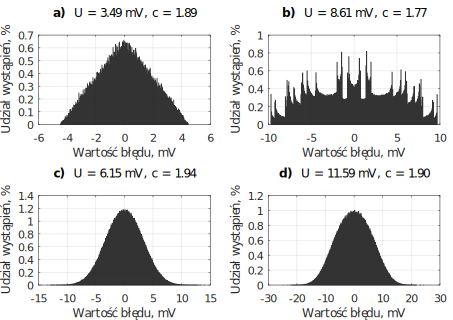
\includegraphics{obrazki/hist_part_a}
\makecaption{fig:symul_parta_hist}{Histogramy realizacji sygnałów błędów \textbf{a)}~statycznego, \textbf{b)}~dynamicznego, \textbf{c)}~losowego, \textbf{d)}~wypadkowego, wielkości wyjściowej analizowanego w eksperymencie symulacyjnym przetwornika pomiarowego uzyskane metodą Monte-Carlo}
\end{center}
\end{figure}

Wyznaczona na drodze eksperymentu wartość wielkości $U_{a,\Sigma}$ wyniosła~\qty{11.58}{mV}, przy czym wartość współczynnika rozszerzenia $c_{a,\Sigma}$ wyniosła $1.90$. Wartość niepewności oszacowana na podstawie równania~\eqref{eq:sym_parta_uncert_value_a} jest zatem około $4.5\%$ większa od wartości uzyskanej na drodze eksperymentu. Należy zaznaczyć, że ta sama wartość wyznaczona za pomocą równania~\eqref{eq:sym_parta_uncert_sum} stosując współczynniki koherencji, których wartości zostały wyznaczone bez użycia zaproponowanej w pracy korekty opisanej równaniem~\eqref{eq:unc_cohercorra} wynosi~\qty{12.41}{mV}, a zatem jest ona o $7.3\%$ większa od wartości referencyjnej. W przypadku wartości oszacowanej na podstawie równania~\eqref{eq:sym_parta_uncert_value_b} rozbieżność jest nieco mniejsza i wynosi około $3.2\%$, co dowodzi że w analizowanym przypadku spełnione zostały założenia związane z centralnym twierdzeniem granicznym, a przyjęte uproszczenia okazały się nie mieć znaczącego wpływu na wynik obliczeń. Uzyskana wartość wariancji sygnału błędu wypadkowego wielkości wyjściowej wyniosła w eksperymencie~\qty{37.1}{\micro V}, co pokrywa się z wartością wyznaczoną w równaniu~\eqref{eq:sym_parta_var_sum}. Wyznaczone w równaniach od~\eqref{eq:sym_parta_uncert_stat} do~\eqref{eq:sym_parta_factor_rand} parametry dla składowych sygnału błędu również w zadowalającym stopniu pokrywają się z uzyskanymi na drodze eksperymentu.

Zastosowana metoda szacowania wartości współczynników koherencji w celu wyznaczenia wypadkowej wartości niepewności rozszerzonej zapewnia wyniki zawyżone o kilka procent w stosunku do wartości uzyskiwanych symulacyjne. Jako, że omawiane rozbieżności są niewielkie oraz ich znak jest dodatni, uzyskiwane wyniki można uznać za prawidłowe. Wadą przedstawionej metody jest jednak konieczność znajomości wartości współczynników kształtu, co powoduje, że dla rozkładów o niestandardowym kształcie jej obszar zastosowań staje się ograniczony. Zaproponowana w pracy dodatkowa korekta wartości współczynników koherencji pozwala na uzyskanie bardziej zbliżonych, do uzyskiwanych symulacyjnie, wyników obliczeń.

Wobec przedstawionych rozważań i wyników przeprowadzonego eksperymentu stwierdzić można, że zaproponowany model błędu odpowiednio opisuje związki pomiędzy kolejnymi sygnałami błędów, zachodzące w analizowanym obiekcie. Jako, że kolejne fragmenty analizowanego toru pomiarowego przetwarzać będą zdefiniowane dotychczas sygnały błędów, przeprowadzony proces wyznaczania parametrów wypadkowych w przypadku grupy błędów dynamicznych oraz wyznaczanie parametrów wypadkowego błędu wielkości wyjściowej był bezzasadny i został przeprowadzony jedynie w celu weryfikacji zaproponowanej metody obliczeń. W przypadku pozostałych grup sygnałów błędów, które cechowały się rozkładami o standardowych kształtach, wyznaczenie wypadkowych parametrów tych sygnałów pozwala na zmniejszenie liczby analizowanych sygnałów i upraszcza dalszą analizę.

\section{Analiza wzmacniacza pomiarowego}

Kolejną część toru pomiarowego stanowi wzmacniacz, którego zadaniem jest dopasowanie poziomu sygnału napięciowego $y_{a}(t)$, reprezentującego mierzoną wielkość fizyczną $s(t)$, do zakresu napięcia wejściowego $y_{b}(t)$ przetwornika analogowo-cyfrowego. Zakładane wzmocnienie układu wynosi $s_{b} = \qty{3.3}{V \per V}$, zatem w przypadku idealnym jego funkcję przetwarzania $\dot{f}_{b}(x)$ stanowi addytywna funkcja liniowa opisana równaniem:
\begin{equation}
\dot{f}_{b} \emb{x} = s_{b} x = 3.3 \cdot x \label{eq:sym_partb_function},
\end{equation}
przy czym przyjmuje się, że nieliniowość przedstawionej charakterystyki jest pomijalnie mała i nie została rozważona w przedstawionym eksperymencie, a zatem przyjąć można założenie, gdzie $\tilde{f}_{b}(x) = \dot{f}_{b}(x)$. Wobec powyższych wielkość wyjściową analizowanego obiektu opisać można jako:
\begin{gather}
\dot{y}_{b} \emb{t} = \dot{f}_{b} \emb{\dot{y}_{a} \emb{t}} = 3.3 \dot{y}_{a} \emb{t} \label{eq:sym_partb_out_ideal}, \\
\tilde{y}_{b} \emb{t} = \dot{y}_{b} \emb{t} + e_{b,\Sigma} \emb{t} \label{eq:sym_partb_out_real},
\end{gather}
gdzie sygnały wchodzące w skład wypadkowego sygnału błędu $e_{b,\Sigma}(t)$ opisano w dalszej części podrozdziału oraz wskazano ich parametry.

Analizowany układ wzmacniacza charakteryzuje się częstotliwością graniczną równą $f_{b,g} = \qty{650}{kHz}$, stąd zakłada się, że jego transmitancje opisać można w postaci:
\begin{equation}
\tilde{G}_{b} \emb{j\omega} = \frac{1}{1 + j \frac{\omega}{2 \pi f_{b,g}}} = \frac{1}{\frac{\omega^{2}}{4 \pi^{2} f_{b,g}^{2}} + 1} - j \frac{\omega}{2 \pi f_{b,g} \left( \frac{\omega^{2}}{4 \pi^{2} f_{b,g}^{2}} + 1 \right) } \label{eq:sym_partb_trans},
\end{equation}
wobec czego równania~\eqref{eq:mid_cont_amp} oraz~\eqref{eq:mid_cont_phi} przyjmują w analizowanym przypadku postać:
\begin{gather}
\tilde{K}_{b} \emb{\omega} = \sqrt{\left( \Re \left( \tilde{G}_{b} \emb{j\omega} \right) \right)^{2} + \left( \Im \left( \tilde{G}_{b} \emb{j\omega} \right) \right)^{2}} = \left( \frac{\omega^{2}}{4 \pi^{2} f_{b,g}^{2}} + 1 \right)^{-\frac{1}{2}} \label{eq:sym_partb_amp_real}, \\
\tilde{\varphi}_{b} \emb{\omega} = \arctan \left( \frac{\Im \left( \tilde{G}_{b} \emb{j\omega} \right)}{\Re \left( \tilde{G}_{b} \emb{j\omega} \right)} \right) = \arctan \left( -\frac{\omega}{2 \pi f_{b,g}} \right) \label{eq:sym_partb_phi_real},
\end{gather}
natomiast w przypadku idealnej transmitancji $\dot{G}_{b}(j\omega) = 1$, parametry te wynoszą kolejno:
\begin{gather}
\dot{K}_{b} \emb{\omega} = \sqrt{\left( \Re \left( \dot{G}_{b} \emb{j\omega} \right) \right)^{2} + \left( \Im \left( \dot{G}_{b} \emb{j\omega} \right) \right)^{2}} = 1 \label{eq:sym_partb_amp_ideal}, \\
\dot{\varphi}_{b} \emb{\omega} = \arctan \left( \frac{\Im \left( \dot{G}_{b} \emb{j\omega} \right)}{\Re \left( \dot{G}_{b} \emb{j\omega} \right)} \right) = 0 \label{eq:sym_partb_phi_ideal}.
\end{gather}

Pierwszą omawianą grupę sygnałów błędów stanowią błędy własne, wprowadzane przez analizowany obiekt. Przyjmuje się, że temperatura otoczenia $\vartheta(t)$ wpływa na dryf zera analizowanego wzmacniacza zgodnie z zależnością opisaną równaniem:
\begin{equation}
f_{b,z} \left( \vartheta \emb{t} \right) = \frac{7}{2} \left( \vartheta \emb{t} - \qty{20}{\degreeCelsius} \right)~\unit{\frac{mV}{K}} \label{eq:sym_partb_temp_err},
\end{equation}
oraz że w czasie wykonywania pojedynczej serii pomiarowej zmiany tej temperatury będą zbliżone do zera. Błąd statyczny własny, wynikający z dryfu zera spowodowanego zmianą temperatury otoczenia, zgodnie z równaniem~\eqref{eq:out_cont_err_env_self} opisać można jako:
\begin{equation}
e_{b,sw} \emb{t} = f_{b,z} \left( \vartheta \emb{t} \right) \label{eq:sym_partb_err_sw}.
\end{equation}
W przypadku właściwości dynamicznych, zdefiniowany w równaniach~\eqref{eq:mid_cont_err_dyn_prop} oraz~\eqref{eq:out_cont_err_dyn_prop} sygnał błędu dynamicznego własnego, w analizowanym przypadku opisać można równaniem:
\begin{equation}
e_{b,dw} \emb{t} = \sum _{i = 1} ^{3} e_{b,dw} \emb{t,\omega_{a,i}} \label{eq:sym_partb_dyn_self_sum}.
\end{equation}
gdzie kolejne harmoniczne przedstawionego sygnału w funkcji pulsacji opisać można na podstawie równań~\eqref{eq:sym_parta_amp_out_ideal} oraz~\eqref{eq:sym_parta_phi_out_ideal} jako:
\begin{equation}
\begin{split}
e_{b,dw} \emb{t,\omega} =~
& \tilde{f}_{b} \left( \tilde{K}_{b} \emb{\omega} E_{a,o} \emb{\omega} \sin \left( \omega t + \varphi_{a,o} \emb{\omega} + \tilde{\varphi}_{b} \emb{\omega} \right) \right)- \\
& \tilde{f}_{b} \left( \dot{K}_{b} \emb{\omega} E_{a,o} \emb{\omega} \sin \left( \omega t + \varphi_{a,o} \emb{\omega} + \dot{\varphi}_{b} \emb{\omega} \right) \right)
\end{split}
\label{eq:sym_partb_dyn_self_err},
\end{equation}
przy czym parametry składowych przetwarzanego sygnału $y_{a}(t)$ dla przypadku idealnego zdefiniowano w równaniach~\eqref{eq:sym_parta_amp_out_ideal} oraz~\eqref{eq:sym_parta_phi_out_ideal}.

Drugą grupę sygnałów błędów stanowią błędy propagowane, przenoszone z wejścia na wyjście obiektu. Sygnały błędu statycznego $e_{a,sw}(t)$, związanego z dryfem zera przetwornika pomiarowego, błędu losowego $e_{a,rw}(t)$, związanego z nieliniowością jego charakterystyki oraz błędu losowego $e_{a,rp}(t)$, związanego z przetwarzanym sygnałem szumu, będą przenoszone zgodnie równaniami~\eqref{eq:out_cont_err_stat_prop} oraz~\eqref{eq:out_cont_err_rand_prop}, a zatem przebieg tych sygnałów na wyjściu analizowanego obiektu można opisać w następujący sposób:
\begin{gather}
e_{b,sp} \emb{t} = \tilde{f}_{b} \left( e_{a,sw} \emb{t} \right) = 3.3 e_{a,sw} \emb{t} \label{eq:sym_partb_stat_prop_err}, \\
e_{b,rp,1} \emb{t} = \tilde{f}_{b} \left( e_{a,rw} \emb{t} \right) = 3.3 e_{a,rw} \emb{t} \label{eq:sym_partb_rand_prop_err_1}, \\
e_{b,rp,2} \emb{t} = \dot{f}_{b} \left( e_{a,rp} \emb{t} \right) = 3.3 e_{a,rp} \emb{t} \label{eq:sym_partb_rand_prop_err_2}.
\end{gather}
na podstawie zależności~\eqref{eq:sym_partb_rand_prop_err_1} oraz~\eqref{eq:sym_partb_rand_prop_err_2} wskazać można zależność opisującą wypadkowy sygnał propagowanego błędu losowego:
\begin{equation}
e_{b,rp} \emb{t} = e_{b,rp,1} \emb{t} + e_{b,rp,2} \emb{t} = 3.3 \left( e_{a,rp} \emb{t} + e_{a,rw} \emb{t} \right) \label{eq:sym_partb_rand_prop_err},
\end{equation}
Analizę propagacji sygnału błędu dynamicznego $e_{a,dw}(t)$ wykonywać należy z osobna dla każdej harmonicznej tego sygnału. Harmoniczne te, zgodnie z charakterystyką dynamiczną analizowanego wzmacniacza, będą odpowiednio tłumione i przesuwane w fazie, a następnie, zgodnie z jego charakterystyką statyczną, zostaną wzmocnione. Przedstawione zależności, zgodnie z równaniami~\eqref{eq:mid_cont_err_dyn_prop} oraz~\eqref{eq:out_cont_err_dyn_prop} przyjmują postać:
\begin{equation}
\begin{split}
e_{b,dp} \emb{t,\omega} =~
& \dot{f}_{b} \left( \tilde{K}_{b} \emb{\omega} E_{a,e} \emb{\omega} \sin \left( \omega t + \varphi_{a,e} \emb{\omega} + \tilde{\varphi}_{b} \emb{\omega} \right) \right) = \\
& 3.3 \tilde{K}_{b} \emb{\omega} E_{a,e} \emb{\omega} \sin \left( \omega t + \varphi_{a,e} \emb{\omega} + \tilde{\varphi}_{b} \emb{\omega} \right) 
\end{split}
\label{eq:sym_partb_dyn_prop_err},
\end{equation}
przy czym parametry przetwarzanych harmonicznych sygnału błędu dynamicznego zestawiono wcześniej w tabeli~\ref{tab:sym_parta_params_dyn_summary}. Wobec powyższych, sygnał błędu dynamicznego propagowanego może być opisany równaniem:
\begin{equation}
e_{b,dp} \emb{t} = \sum _{j = 1} ^{3} e_{b,dp} \emb{t,\omega_{a,j}} \label{eq:sym_partb_dyn_prop_sum}.
\end{equation}

Na podstawie przedstawionych zależności od~\eqref{eq:sym_partb_err_sw} do~\eqref{eq:sym_partb_dyn_prop_sum}, zgodnie z równaniem~\eqref{eq:out_cont_err_sum_all}, opisać można wypadkowy błąd wielkości wyjściowej analizowanego wzmacniacza pomiarowego w postaci sumy wymienionych sygnałów błędów:
\begin{equation}
e_{b,\Sigma} \emb{t} = e_{b,sw} \emb{t} + e_{b,sp} \emb{t} + e_{b,rp} \emb{t} + e_{b,dw} \emb{t} + e_{b,dp} \emb{t} \label{eq:sym_partb_error_sum}.
\end{equation}

Kolejny etap analizy prowadzi do wyznaczenia parametrów wariancji opisanych sygnałów błędów. W przypadku sygnałów błędów dynamicznych należy, analogicznie jak w przypadku przedstawionej analizy przetwornika pomiarowego, wyznaczyć wypadkowe amplitudy i przesunięcia w fazie kolejnych harmonicznych sygnału błędu. W analizowanym przypadku każda wypadkowa harmoniczna sygnału błędu dynamicznego złożona będzie z trzech składników -- dwóch wynikających z równania~\eqref{eq:sym_partb_dyn_self_err} oraz jednej wynikającej z równania~\eqref{eq:sym_partb_dyn_prop_err}. Należy zauważyć, że omawiane parametry wyznaczać można również na podstawie tabeli~\ref{tab:sym_parta_params_dyn_list}, natomiast dla zachowania czytelności przykładu przedstawiane obliczenia były przeprowadzane dla wyprowadzonych wcześniej wypadkowych wartości parametrów analizowanych harmonicznych sygnału błędu dynamicznego. Parametry wypadkowe należy wyznaczyć zgodnie z metodą opisaną w równaniach od~\eqref{eq:dyn_vect} do~\eqref{eq:dyn_vect_phi}. Wyznaczone analogicznie do przykładu opisanego w równaniach od~\eqref{eq:sym_parta_dyn_self_example_sum} do~\eqref{eq:sym_parta_dyn_self_example_phi} parametry wypadkowe sygnału błędu dynamicznego $e_{b,d}$ zestawiono w tabeli~\ref{tab:sym_partb_params_dyn_summary}, natomiast tabela~\ref{tab:sym_partb_params_unc_list} przedstawia budżet niepewności wielkości wyjściowej analizowanego wzmacniacza pomiarowego z uwzględnieniem podziału na błędy własne i propagowane.

Sygnał błędu losowego $e_{b,rp,2}(t)$ związany z szumem obecnym w sygnale pomiarowym, należy analizować zgodnie z zależnościami~\eqref{eq:mid_cont_var_omega}, \eqref{eq:mid_cont_var_rand} oraz~\eqref{eq:out_cont_err_rand_prop}. Podobnie, jak w przypadku analizowanego przetwornika pomiarowego, w zakresie częstotliwości Nyquista transmitancja obiektu nie wpływa na widmo przetwarzanego sygnału szumu $e_{a,rp}(t)$. Można zatem, zgodnie z zależnością~\eqref{eq:out_cont_err_rand_prop}, zapisać równanie opisujące przebieg omawianego sygnału błędu na wyjściu obiektu:
oraz 

\begin{table}[htb!]
\begin{center}
\makecaption{tab:sym_partb_params_dyn_summary}{Parametry wypadkowe kolejnych harmonicznych błędu dynamicznego analizowanego w eksperymencie symulacyjnym wzmacniacza pomiarowego}
\begin{tabular}[c]{| c | c | S[table-format = 2.2] | S[table-format = +1.2] |} \hline
\textbf{Lp. $j$} & \textbf{Pulsacja $\omega_{b,j}$, rad/s} & \textbf{Amplituda $E_{b,e}(\omega_{b,j})$, mV} & \textbf{Faza $\varphi_{b,e}(\omega_{b,j})$, rad} \\ \hline
1 & $1000  \cdot 2\pi$  &   9.23  & -1.57  \\ \hline
2 & $5000  \cdot 2\pi$  &  23.08  &  1.96  \\ \hline
3 & $15000 \cdot 2\pi$  &  23.07  & -1.07  \\ \hline
\end{tabular}
\end{center}
\end{table}

\begin{table}[htb!]
\begin{center}
\makecaption{tab:sym_partb_params_unc_list}{Budżet niepewności wielkości wyjściowej analizowanego w eksperymencie symulacyjnym wzmacniacza pomiarowego, gdzie (a)~oznacza przetwornik pomiarowy oraz (b)~oznacza wzmacniacz pomiarowy}
\begin{tabular}[c]{| c | c | S[table-format = 2.2] | S[table-format = 3.2] | c | c |} \hline
\textbf{Lp.} & \textbf{Symbol} & \textbf{$U_{95\%}$, mV} & \textbf{$\sigma^{2}$, \micro V} & \textbf{Rozkład} & \textbf{Źródło błędu} \\ \hline
1  & ${b,sw}$       & 11.52 &  36.75  & trójkątny                    & dryf temperatury (a)                       \\ \hline
2  & ${b,sp}$       & 8.15  &  18.38  & trójkątny                    & dryf temperatury (b)                       \\ \hline
3  & ${b,rp,1}$     & 9.93  &  36.26  & jednostajny                  & nieliniowość obiektu (a)                   \\ \hline
4  & ${b,rp,2}$     & 16.70 &  72.64  & normalny                     & szum wielkości wejściowej                  \\ \hline
5  & ${b,dp,1}$     & 6.21  &  19.14  & \multirow{6}{*}{dwumodalny}  & \multirow{3}{*}{transmitancja (a)}         \\ \cline{1-4}
6  & ${b,dp,2}$     & 15.53 &  119.62 &                              &                                            \\ \cline{1-4}
7  & ${b,dp,3}$     & 15.52 &  119.44 &                              &                                            \\ \cline{1-4} \cline{6-6}
8  & ${b,dw,1}$     & 3.06  &  4.64   &                              & \multirow{3}{*}{transmitancja (b)}         \\ \cline{1-4}
9  & ${b,dw,2}$     & 7.65  &  29.00  &                              &                                            \\ \cline{1-4}
10 & ${b,dw,3}$     & 7.65  &  28.99  &                              &                                            \\ \hline
\end{tabular}
\end{center}
\end{table}

Ostatnim krokiem analizy pozostaje określenie związków pomiędzy składowymi budżetu niepewności zestawionymi w tabeli~\ref{tab:sym_partb_params_unc_list}. Należy zauważyć, że składowe związane z dryfem temperaturowym przetwornika pomiarowego oraz dryfem temperaturowym wzmacniacza zależą od tej samej wielkości fizycznej -- temperatury otoczenia. Oznacza to, że należy określić korelacje pomiędzy omawianymi wielkościami zgodnie z zależnością~\eqref{eq:var_corr} i uwzględnić ją w równaniu~\eqref{eq:var_matrix} w celu określenia wypadkowej wariancji składanych sygnałów błędu. Wyznaczony współczynnik korelacji pomiędzy opisywanymi błędami statycznymi wynosi:
\begin{equation}
r_{b,sw,sp} = \frac{\sigma_{b,sw,sp}^{2} - \sigma_{b,sw}^{2} - \sigma_{b,sp}^{2}}{2 \sigma_{b,sw} \sigma_{b,sp}} = \frac{\num{1.07e-4} - \num{3.68e-5} - \num{1.84e-5}}{2 \cdot \num{6.06e-3} \cdot \num{4.29e-3}} = 1.00 \label{eq:sym_partb_stat_corr},
\end{equation}
przy czym w celu wyznaczenia wypadkowej wartości wariancji $\sigma_{b,sw,sp}^{2}$ przeprowadzono eksperyment metodą Monte-Carlo. Ze względu na fakt, że analizowane sygnały błędu statycznego zależą liniowo w pełni od tej samej wielkości fizycznej, rozkład błędu wypadkowego cechować się będzie kształtem identycznym, jak rozkład omawianej wielkości fizycznej. W przypadku kolejnych harmonicznych błędu dynamicznego własnego oraz propagowanego zauważyć można, że przesunięcia fazowe przebiegów tych harmonicznych są pomijalnie małe -- ich rząd wielkości wynosi~\qty{1e-3}{rad}. Można zatem przyjąć, że współczynniki korelacji składanych sygnałów będą zbliżone do jedności, co pozwoli zastosować równanie~\eqref{eq:var_matrix} do określenia wypadkowej wariancji tych przebiegów. Założenia te potwierdzają wyniki zestawione w tabeli~\ref{tab:sym_partb_params_dyn_summary}.

Wobec przedstawionych zależności, wariancję oraz niepewność rozszerzoną wypadkowego błędu statycznego, będącego sumą skorelowanych sygnałów błędu statycznego własnego i propagowanego, opisują równania~\eqref{eq:var_matrix} oraz~\eqref{eq:unc_matrix} wyrażone w analizowanym przypadku jako:
\begin{gather}
\begin{split}
\sigma_{b,s}^{2} = ~ &
\begin{bmatrix}
\sigma_{b,sw} \\ \sigma_{b,sp}
\end{bmatrix}^{T}
\begin{bmatrix}
1 & r_{b,sw,sp} \\
r_{b,sp,rw} & 1
\end{bmatrix}
\begin{bmatrix}
\sigma_{b,sw} \\ \sigma_{b,sp}
\end{bmatrix} = \\ &
\begin{bmatrix}
\num{6.06e-3} \\ \num{4.29e-3}
\end{bmatrix}^{T}
\begin{bmatrix}
1 & 1 \\
1 & 1
\end{bmatrix}
\begin{bmatrix}
\num{6.06e-3} \\ \num{4.29e-3}
\end{bmatrix} = \qty{107.12}{\micro V}
\end{split}
\label{eq:sym_partb_stat_var}. \\
\begin{split}
U_{b,s} = ~ & \sqrt{
\begin{bmatrix}
U_{b,sw} \\ U_{b,sp}
\end{bmatrix}^{T}
\begin{bmatrix}
1 & h_{b,sw,sp} \\
h_{b,sp,rw} & 1
\end{bmatrix}
\begin{bmatrix}
U_{b,sw} \\ U_{b,sp}
\end{bmatrix}} = \\ & \sqrt{
\begin{bmatrix}
\num{11.52e-3} \\ \num{8.15e-3}
\end{bmatrix}^{T}
\begin{bmatrix}
1 & 1 \\
1 & 1
\end{bmatrix}
\begin{bmatrix}
\num{11.52e-3} \\ \num{8.15e-3}
\end{bmatrix}} = \qty{19.67}{mV}
\end{split}
\label{eq:sym_partb_stat_uncert},
\end{gather}
gdzie współczynniki koherencji $h_{b,sw,sp}$ w przypadku pełnej dodatniej korelacji, jaka ma miejsce zgodnie z równaniem~\eqref{eq:sym_partb_stat_corr}, przyjmują wartość jedności. W przypadku sygnałów błędów losowych propagowanych korelacja nie występuje, a zatem wariancja wypadkowego sygnału błędu losowego jest wyznaczana zgodnie z zależnością~\eqref{eq:var_sum} jako:
\begin{equation}
\sigma_{b,r}^{2} = \sigma_{b,rp,1}^{2} + \sigma_{b,rp,2}^{2} = \qty{108.90}{\micro V} \label{eq:sym_partb_rand_var}.
\end{equation}
Wypadkową niepewność rozszerzoną w analizowanym przypadku wyznaczyć można zgodnie z równaniem~\eqref{eq:unc_sum}, przy czym:
\begin{gather}
\begin{split}
U_{a,r} = ~ & \sqrt{
\begin{bmatrix}
U_{a,rp,1} \\ U_{b,rp,2}
\end{bmatrix}^{T}
\begin{bmatrix}
1            & h_{a,rp,1,2} \\
h_{a,rp,2,1} & 1
\end{bmatrix}
\begin{bmatrix}
U_{a,rp,1} \\ U_{b,rp,2}
\end{bmatrix}} = ~ \\ & \sqrt{
\begin{bmatrix}
\num{9.93e-3} \\ \num{16.70e-3}
\end{bmatrix}^{T}
\begin{bmatrix}
1.000 & 0.120 \\
0.120 & 1.000
\end{bmatrix}
\begin{bmatrix}
\num{9.93e-3} \\ \num{16.70e-3}
\end{bmatrix}} = \qty{20.43}{mV}
\end{split}
\label{eq:sym_partb_rand_uncert}, \\
h_{b,rp,1,2} = s_{u,n} \cdot \sqrt{\frac{\num{9.93e-3}}{\num{16.70e-3}}} \left( \frac{\emb{\num{9.93e-3}}^{2} + \emb{\num{16.70e-3}}^{2}}{\num{377.49e-6}} \right) = 0.120 \label{eq:sym_partb_coher_rp_1_2}.
\end{gather}

Korzystając zależności przedstawionych równaniami od~\eqref{eq:sym_partb_stat_var} do~\eqref{eq:sym_partb_rand_uncert}, zestawionych w tabeli~\ref{tab:sym_partb_params_unc_list} wartości oraz równania~\eqref{eq:var_function}, sporządzono budżet niepewności uwzględniający podział na kategorie błędów i zestawiono go w tabeli~\ref{tab:sym_partb_params_unc_sum}. Ze względu na konieczność przeprowadzania dalszej analizy w dziedzinie pulsacji, nie wyznaczano wypadkowych parametrów błędu dynamicznego oraz parametrów wypadkowego sygnału błędu wielkości wyjściowej $y_{b}(t)$. Przedstawione wartości posłużą do analizy właściwości metrologicznych kolejnych fragmentów toru pomiarowego.

\begin{table}[htb!]
\begin{center}
\makecaption{tab:sym_partb_params_unc_sum}{Budżet niepewności wielkości wyjściowej analizowanego w eksperymencie symulacyjnym wzmacniacza pomiarowego z uwzględnieniem podziału na błędy statyczne, dynamiczne oraz losowe}
\begin{tabular}[c]{| c | c | S[table-format = 2.2] | S[table-format = 3.2] | c | c |} \hline
\textbf{Lp.} & \textbf{Symbol} & \textbf{$U_{95\%}$, mV} & \textbf{$\sigma^{2}$, \micro V} & \textbf{Rozkład} & \textbf{Źródło błędu} \\ \hline
1 & ${b,s}$        & 19.67 &  107.12 & trójkątny                    & wypadkowy dryf temperatury                 \\ \hline
2 & ${b,r}$        & 20.43 &  108.90 & normalny                     & szum i nieliniowość obiektu                \\ \hline
3 & ${b,d,1}$      & 9.20  &  42.60  & \multirow{3}{*}{dwumodalny}  & \multirow{3}{*}{wypadkowa transmitancja}   \\ \cline{1-4}
4 & ${b,d,2}$      & 23.01 &  266.34 &                              &                                            \\ \cline{1-4}
5 & ${b,d,3}$      & 23.00 &  266.11 &                              &                                            \\ \hline
\end{tabular}
\end{center}
\end{table}

W celu weryfikacji poprawności zastosowanego modelu błędu oraz przeprowadzonych obliczeń wykonano eksperyment metodą Monte-Carlo, polegający na wyznaczeniu sto tysięcy razy wartości wielkości wyjściowej analizowanego wzmacniacza pomiarowego. Podczas eksperymentu fazę sygnału wejściowego $s(t)$ losowano z przedziału $<-2 \pi f_{1};2 \pi f_{1}>\unit{rad}$, przy czym wylosowanie każdej w możliwych wartości było jednakowo prawdopodobne. Uzyskiwaną wartość wielkości wyjściowej porównywano z wartością otrzymaną dla idealnej realizacji analizowanego fragmentu toru pomiarowego (tj. takiej, w której nie występowały żadne źródła błędów), a następnie na podstawie równania~\eqref{eq:sym_partb_error_sum} wyznaczano realizację błędu wielkości wyjściowej $y_{b}(t)$. Wyznaczone wartości zostały użyte do sporządzenia histogramu, na podstawie którego zgodnie z równaniem~\eqref{eq:unc_summation} określono parametry rozkładu błędu analizowanej wielkości wyjściowej. Eksperyment wykonano uwzględniając wszystkie źródła błędu oraz uwzględniając źródła związane z kolejnymi kategoriami błędów. Uzyskane na drodze eksperymentu histogramy przedstawia rysunek~\ref{fig:symul_partb_hist}.

\begin{figure}[htb!]
\begin{center}
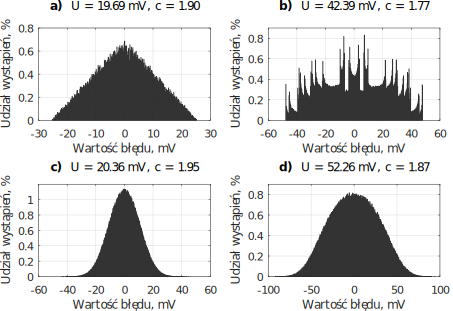
\includegraphics{obrazki/hist_part_b}
\makecaption{fig:symul_partb_hist}{Histogramy błędów \textbf{a)}~statycznego, \textbf{b)}~dynamicznego, \textbf{c)}~losowego, \textbf{d)}~wypadkowego, wielkości wyjściowej analizowanego w eksperymencie symulacyjnym wzmacniacza pomiarowego uzyskane metodą Monte-Carlo}
\end{center}
\end{figure}

Analizując wyniki eksperymentu zauważyć można, że uzyskane wartości dla sygnałów błędów losowego oraz statycznego są zbliżone do tych przedstawionych w tabeli~\ref{tab:sym_partb_params_unc_sum}. Pozwala to zakładać, że podobnie jak w przypadku analizy właściwości przetwornika pomiarowego, przyjęty model błędu oraz stosowane zależności poprawnie określają związki pomiędzy wskazanymi błędami i umożliwiają poprawne oszacowanie ich parametrów. Na etapie przeprowadzonej analizy nie wyznaczano wypadkowych parametrów błędu dynamicznego oraz całkowitego błędu wypadkowego -- dane te, jak pokazano na obecnym przykładzie, nie są użyteczne podczas analizy kolejnych fragmentów toru pomiarowego.

\section{Analiza przetwornika analogowo-cyfrowego}

Kolejnym elementem wchodzącym w skład analizowanego toru pomiarowego jest przetwornik analogowo-cyfrowy. W eksperymencie zakłada się, że element jest realizowany przy użyciu 8-bitowego przetwornika wagowego o zakresie napięcia wejściowego z przedziału $<-3;3>\unit{V}$. Wobec powyższych liczba dostępnych wartości wielkości wyjściowej tego przetwornika wynosi $N_{q} = 256$, natomiast wartość kwantu jest równa $q = \frac{3 - (-3)~\unit{V}}{256} = \qty{23.44}{mV}$. Zakładając, że wielkością wyjściową $x_{c}(n)$ analizowanego przetwornika będzie dyskretna reprezentacja wielkości wejściowej $y_{b}(t)$, zapisać można na podstawie równań od~\eqref{eq:out_cont_ideal_all} do~\eqref{eq:out_cont_err_sum_all} następujące zależności:
\begin{gather}
\dot{x}_{c} \emb{n} = \dot{y}_{b} \emb{nT_{p}} \label{eq:sym_partc_out_ideal}, \\
\tilde{x}_{c} \emb{n} = \tilde{y}_{b} \emb{nT_{p}} + e_{c,q} \left( \tilde{y}_{b} \emb{nT_{p}} \right) = \dot{x}_{c} \emb{n} + e_{c,\Sigma} \emb{n} \label{eq:sym_partc_out_real}, \\
e_{c,\Sigma} \emb{n} = e_{b,\Sigma} \emb{nT_{p}} + e_{c,q} \left( \tilde{y}_{b} \emb{nT_{p}} \right) \label{eq:sym_partc_error_sum},
\end{gather}
gdzie $T_{p}$ jest okresem próbkowania równym $\frac{1}{\qty{48}{kHz}} = \qty{20.8(3)}{\micro s}$.
Na podstawie zależności danych równaniami od~\eqref{eq:adc_function} do~\eqref{eq:adc_qerrrange} zapisać można nierówność określającą przedział, w jakim znajdować się będą wartości błędu kwantowania $e_{c,q}(x)$ jako:
\begin{equation}
\qty{-11.72}{mV} \le e_{c,q} \emb{x} \le \qty{11.72}{mV} \label{eq:sym_partc_error_quant}.
\end{equation}

Analizując równanie~\eqref{eq:sym_partc_out_real} zauważyć można, że realizacja błędu kwantowania zależna jest od wartości przetwarzanej wielkości wejściowej analizowanego przetwornika. Jednakże, jak wykazano w pracach~\cite{sienkowski_kwant, sienkowski_adc}, zależność tą można pominąć. Przy założeniu, że uzyskanie na wejściu przetwornika dowolnej wartości z zakresu wartości wielkości wejściowej jest jednakowo prawdopodobne oraz że podczas pomiaru wielkość ta będzie się zmieniać, powtarzając proces pomiaru wielokrotnie, z punktu widzenia pojedynczego okna pomiarowego, błąd kwantowania $e_{c,q}(x)$ rozpatrywać można w kategoriach probabilistycznych jako losową realizację wielkości z zakresu opisanego równaniem~\eqref{eq:sym_partc_error_quant} o rozkładzie jednostajnym~\cite{jakubiec_system}. Takie podejście umożliwia zastosowanie zaproponowanego w pracy modelu błędu, podczas gdy analiza zakładająca funkcję przetwarzania omawianego obiektu daną w postaci równania~\eqref{eq:adc_output} byłaby skomplikowana. Wobec powyższych założeń wariancja $\sigma_{c,rw,q}^{2}$ oraz niepewność rozszerzona $U_{c,rw,q}$ związane z błędem kwantowania $e_{c,q}(x)$ mogą być opisane w postaci:
\begin{gather}
\sigma_{c,rw,q}^{2} = \frac{ q^{2}}{12} = \frac{\emb{\num{23.44e-3}}^{2} }{12} = \qty{45.78}{\micro V} \label{eq:sym_partc_var_quant}, \\
U_{c,rw,q} = c_{u} \cdot \sigma_{c,rw,q} = 1.65 \cdot \num{6.77e-3} = \qty{11.16}{mV} \label{eq:sym_partc_uncert_quant}.
\end{gather}

Aby zweryfikować poprawność przedstawionych zależności przeprowadzono eksperyment stosując metodę Monte-Carlo. W ramach eksperymentu wyznaczono sto tysięcy razy realizację wartości wielkości wyjściowej analizowanego przetwornika analogowo-cyfrowego, a następnie jej wartość porównano z wartością idealną, uzyskaną dla toru pomiarowego w którym nie występowały żadne źródła błędów. Na podstawie uzyskanych zgodnie z równaniem~\eqref{eq:sym_partc_error_sum} realizacji błędu opracowano histogram i określono jego parametry. Identyczny eksperyment przeprowadzono ponownie, z tą różnicą, że jako jedyne źródło błędów, uwzględniono w nim jedynie obecność procesu kwantowania w celu oszacowania jedynie parametrów błędu kwantowania. Rysunek~\ref{fig:symul_partc_hist} przedstawia uzyskane na drodze eksperymentu histogramy.

\begin{figure}[htb!]
\begin{center}
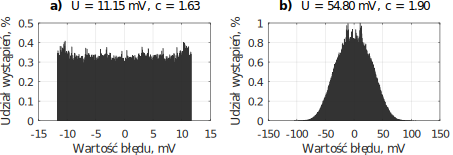
\includegraphics{obrazki/hist_part_c}
\makecaption{fig:symul_partc_hist}{Histogramy błędów \textbf{a)}~kwantowania, \textbf{b)}~wypadkowego, wielkości wyjściowej analizowanego w eksperymencie symulacyjnym przetwornika analogowo-cyfrowego uzyskane metodą Monte-Carlo}
\end{center}
\end{figure}

Analizując wyniki poprzedniego eksperymentu, przedstawione na rysunku~\ref{fig:symul_partb_hist}, oraz wyniki bieżącego eksperymentu, przedstawione na rysunku~\ref{fig:symul_partc_hist}, wnioskować można że zaproponowane wcześniej założenia są spełnione. Wariancja błędu wypadkowego $\sigma_{b,\Sigma}^{2}$ wielkości wejściowej przetwornika analogowo-cyfrowego wyniosła w poprzednim eksperymencie~\qty{788.18}{\micro V}. Wariancja błędu wypadkowego $\sigma_{c,\Sigma}^{2}$ wielkości wyjściowej przetwornika analogowo-cyfrowego wyniosła w bieżącym eksperymencie~\qty{835.18}{\micro V}, wartość wariancji błędu kwantowania $\sigma_{c,rw,q}^{2}$ wyniosła~\qty{46.88}{\micro V}, natomiast związana z nią niepewność rozszerzona $U_{c,rw,q}$ wyniosła~\qty{11.16}{mV}. Uzyskane wartości w zadowalającym stopniu pokrywają się z wartościami wyznaczonymi na podstawie równań~\eqref{eq:sym_partc_var_quant} oraz~\eqref{eq:sym_partc_uncert_quant}. Przedstawione wartości pozwalają określić korelacje pomiędzy wariancją błędu wypadkowego wielkości wejściowej przetwornika analogowo-cyfrowego oraz wariancją błędu kwantowania na podstawie równania~\eqref{eq:var_corr}, przy czym:
\begin{equation}
r_{c,rw,q;b,\Sigma} = \frac{\sigma_{c,\Sigma}^{2} - \sigma_{c,rw,q}^{2} - \sigma_{b,\Sigma}^{2}}{2 \sigma_{c,rw,q} \sigma_{b,\Sigma}} = \frac{\num{8.4e-4} - \num{4.7e-5} - \num{7.9e-4}}{2 \cdot \num{6.85e-3} \cdot \num{2.81e-2}} = \num{7.8e-4} \label{eq:sym_partc_corr}.
\end{equation}
Uzyskana wartość współczynnika korelacji oraz wyniki przeprowadzonych eksperymentów świadczą o prawidłowości przyjętych założeń i pomijalnie małej korelacji błędu kwantowania z przebiegiem przetwarzanego przez analizowany obiekt sygnału oraz zawartych w nim sygnałów błędów. Wobec powyższych założyć można, że przenoszone z wejścia na wyjście analizowanego obiektu sygnały błędów przenoszone będą w stosunku 1:1, a zatem zachowają one swoje oryginalne parametry oraz zostaną opisane jako błędy propagowane. Na podstawie przedstawionych zależności oraz tabeli~\ref{tab:sym_partb_params_unc_list} sporządzono kompletny budżet niepewności wielkości wyjściowej $x_{c}(n)$ analizowanego przetwornika analogowo-cyfrowego, który zestawiono w tabeli~\ref{tab:sym_partc_params_unc_list}.

\begin{table}[htb!]
\begin{center}
\makecaption{tab:sym_partc_params_unc_list}{Budżet niepewności wielkości wyjściowej analizowanego w eksperymencie symulacyjnym przetwornika analogowo-cyfrowego, gdzie (a) oznacza przetwornik pomiarowy, (b) oznacza wzmacniacz pomiarowy oraz (c) oznacza przetwornik analogowo-cyfrowy}
\begin{tabular}[c]{| c | c | S[table-format = 2.2] | S[table-format = 3.2] | c | c |} \hline
\textbf{Lp.} & \textbf{Symbol} & \textbf{$U_{95\%}$, mV} & \textbf{$\sigma^{2}$, \micro V} & \textbf{Rozkład} & \textbf{Źródło błędu} \\ \hline
1  & ${c,rw,q}$     & 11.16 &  45.78  & jednostajny                  & proces kwantowania (c)                     \\ \hline
2  & ${c,sp,1}$     & 11.52 &  36.75  & trójkątny                    & dryf temperatury (a)                       \\ \hline
3  & ${c,sp,2}$     & 8.15  &  18.38  & trójkątny                    & dryf temperatury (b)                       \\ \hline
4  & ${c,rp,1}$     & 9.93  &  36.26  & jednostajny                  & nieliniowość obiektu (a)                   \\ \hline
5  & ${c,rp,2}$     & 16.70 &  72.64  & normalny                     & szum wielkości wejściowej                  \\ \hline
6  & ${c,dp,a,1}$   & 6.21  &  19.14  & \multirow{6}{*}{dwumodalny}  & \multirow{3}{*}{transmitancja (a)}         \\ \cline{1-4}
7  & ${c,dp,a,2}$   & 15.53 &  119.62 &                              &                                            \\ \cline{1-4}
8  & ${c,dp,a,3}$   & 15.52 &  119.44 &                              &                                            \\ \cline{1-4} \cline{6-6}
9  & ${c,dp,b,1}$   & 3.06  &  4.64   &                              & \multirow{3}{*}{transmitancja (b)}         \\ \cline{1-4}
10 & ${c,dp,b,2}$   & 7.65  &  29.00  &                              &                                            \\ \cline{1-4}
11 & ${c,dp,b,3}$   & 7.65  &  28.99  &                              &                                            \\ \hline
\end{tabular}
\end{center}
\end{table}

Przedstawiony w tabeli~\ref{tab:sym_partc_params_unc_list} budżet niepewności dobrze obrazuje źródła błędów występujące w analizowanym torze pomiarowym oraz jednoznacznie wskazuje ich parametry. Na dalszym etapie analizy stosowanie przedstawionego zestawienia jest jednak kłopotliwe, ponieważ wiązać się będzie z koniecznością analizy każdego ze wskazanych sygnałów błędu z osobna. Ze względu na fakt, że proponowany w pracy model błędu dotyczący kolejnego fragmentu toru pomiarowego, jakim jest algorytm transformacji falkowej, wymaga jedynie określenia wariancji wypadkowego błędu statycznego, losowego oraz wypadkowych wariancji kolejnych harmonicznych błędu dynamicznego, przedstawiony zostanie budżet niepewności uwzględniający opisywany podział, podobnie jak to miało miejsce w przypadku poprzedniego elementu analizowanego toru pomiarowego.

Parametry opisujące wypadkowy błąd losowy wyznaczyć można zgodnie z równaniami~\eqref{eq:var_sum} oraz~\eqref{eq:unc_matrix} które w obecnym przypadku przyjmują postać:
\begin{gather}
\sigma_{c,r}^{2} = \sigma_{c,rp,1}^{2} + \sigma_{c,rp,2}^{2} + \sigma_{c,q}^{2} = \sigma_{b,rp,1}^{2} + \sigma_{b,rp,2}^{2} + \sigma_{c,q}^{2} = \qty{154.68}{\micro V} \label{eq:sym_partc_rand_var}, \\
\begin{split}
U_{c,r} = ~ & \sqrt{
\begin{bmatrix}
U_{c,rp,1} \\ U_{c,rp,2} \\ U_{c,q}
\end{bmatrix}^{T}
\begin{bmatrix}
1            & h_{c,rp,1,2} & h_{c,rp,1,q} \\
h_{c,rp,2,1} & 1            & h_{c,rp,2,q} \\
h_{c,q,rp,1} & h_{c,q,rp,2} & 1
\end{bmatrix}
\begin{bmatrix}
U_{c,rp,1} \\ U_{c,rp,2} \\ U_{c,q}
\end{bmatrix}} = ~ \\ & \sqrt{
\begin{bmatrix}
\num{9.93e-3} \\ \num{16.70e-3} \\ \num{11.16e-3}
\end{bmatrix}^{T}
\begin{bmatrix}
1.000 & 0.091 & 0.141 \\
0.091 & 1.000 & 0.103 \\
0.141 & 0.103 & 1.000
\end{bmatrix}
\begin{bmatrix}
\num{9.93e-3} \\ \num{16.70e-3} \\ \num{11.16e-3}
\end{bmatrix}} = \qty{24.53}{mV}
\end{split}
\label{eq:sym_partc_rand_uncert}, \\
h_{c,rp,1,2} = s_{u,n} \cdot \sqrt{\frac{\num{9.93e-3}}{\num{16.70e-3}}} \left( \frac{\emb{\num{9.93e-3}}^{2} + \emb{\num{16.70e-3}}^{2}}{\num{502.04e-6}} \right) = 0.091 \label{eq:sym_partc_coher_rp_1_2}, \\
h_{c,q,rp,1} = s_{u,u} \cdot \sqrt{\frac{\num{9.93e-3}}{\num{11.16e-3}}} \left( \frac{\emb{\num{9.93e-3}}^{2} + \emb{\num{11.16e-3}}^{2}}{\num{502.04e-6}} \right) = 0.141 \label{eq:sym_partc_coher_q_rp_1}, \\
h_{c,q,rp,2} = s_{u,n} \cdot \sqrt{\frac{\num{11.16e-3}}{\num{16.70e-3}}} \left( \frac{\emb{\num{11.16e-3}}^{2} + \emb{\num{16.70e-3}}^{2}}{\num{502.04e-6}} \right) = 0.103 \label{eq:sym_partc_coher_q_rp_2}, \\
c_{c,r} = \frac{U_{c,r}}{\sigma_{c,r}} = \frac{\num{24.53e-3}}{\num{12.44e-3}} = 1.97 \label{eq:sym_partc_rand_factor}.
\end{gather}

Na podstawie wyznaczonej w równaniu~\eqref{eq:sym_partc_rand_factor} wartości współczynnika rozszerzenia oraz ze względu na spełnienie w analizowanym przypadku warunków centralnego twierdzenia granicznego, zakładać można normalny rozkład wypadkowego sygnału błędu losowego. Biorąc pod uwagę przedstawione dotychczas założenia, wyniki zawarte w tabelach~\ref{tab:sym_partb_params_unc_sum} oraz~\ref{tab:sym_partc_params_unc_list}, jak również wyniki obliczeń przedstawionych w równaniach~\eqref{eq:sym_partc_rand_var} oraz~\eqref{eq:sym_partc_rand_uncert}, sporządzono budżet niepewności z uwzględnieniem omawianego wcześniej podziału, który zestawiono w tabeli~\ref{tab:sym_partc_params_unc_sum}.

\begin{table}[htb!]
\begin{center}
\makecaption{tab:sym_partc_params_unc_sum}{Budżet niepewności wielkości wyjściowej analizowanego w eksperymencie symulacyjnym wzmacniacza przetwornika analogowo-cyfrowego z uwzględnieniem podziału na błędy statyczne, dynamiczne oraz losowe}
\begin{tabular}[c]{| c | c | S[table-format = 2.2] | S[table-format = 3.2] | c | c |} \hline
\textbf{Lp.} & \textbf{Symbol} & \textbf{$U_{95\%}$, mV} & \textbf{$\sigma^{2}$, \micro V} & \textbf{Rozkład} & \textbf{Źródło błędu} \\ \hline
1 & ${c,s}$        & 19.67 &  107.12 & trójkątny                    & wypadkowy dryf temperatury                 \\ \hline
2 & ${c,r}$        & 24.53 &  154.68 & normalny                     & szum, nieliniowość, konwersja              \\ \hline
3 & ${c,d,1}$      & 9.20  &  42.60  & \multirow{3}{*}{dwumodalny}  & \multirow{3}{*}{wypadkowa transmitancja}   \\ \cline{1-4}
4 & ${c,d,2}$      & 23.01 &  266.34 &                              &                                            \\ \cline{1-4}
5 & ${c,d,3}$      & 23.00 &  266.11 &                              &                                            \\ \hline
\end{tabular}
\end{center}
\end{table}

\section{Analiza algorytmu transformacji falkowej}

Ostatnim fragmentem analizowanego toru pomiarowego, a za razem najistotniejszym obiektem z punktu widzenia niniejszej pracy, jest algorytm dyskretnej transformacji falkowej. Zakłada się, że na wejście algorytmu podawany będzie wektor wielkości wejściowych $\mathbf{x}_{d}$ złożony z kolejnych $N = 8$ próbek wielkości wyjściowych $x_{c}(n)$ przetwornika analogowo-cyfrowego. Na wyjściu algorytmu każdorazowo wypracowany zostanie wektor $\mathbf{X}$ zawierający $M = 8$ wielkości wyjściowych algorytmu, które stanowić będą ostateczne wielkości wyjściowe analizowanego toru pomiarowego. Omawiany algorytm wykorzystywać będzie falkę \enquote{db2}, przy czym na jego realizację składać się będą dwie iteracje procesu dekompozycji sygnału. Macierz transformacji $\mathbf{A}$ omawianego algorytmu przedstawia równanie~\eqref{eq:db2_2_8_matrix}. Implementacja stosowanego algorytmu wykorzystywać będzie liczby zmiennoprzecinkowe o długości słowa 16-bitów.

Wobec powyższych założeń oraz modelu zaproponowanego w równaniach od~\eqref{eq:alg_out_mat} do~\eqref{eq:alg_out_single} wektor wielkości wejściowych analizowanego algorytmu opisać można w postaci:
\begin{gather}
\dot{\mathbf{x}}_{d}^{T} \emb{k} =
\begin{bmatrix}
\dot{x}_{c} \emb{kT_{p}} & \dot{x}_{c} \left( \emb{k+1} T_{p} \right) & \hdots & \dot{x}_{c} \left( \emb{k+7} T_{p} \right)
\end{bmatrix}
\label{eq:sym_partd_input_ideal}, \\
\tilde{\mathbf{x}}_{d}^{T} \emb{k} =
\begin{bmatrix}
\tilde{x}_{c} \emb{kT_{p}} & \tilde{x}_{c} \left( \emb{k+1} T_{p} \right) & \hdots & \tilde{x}_{c} \left( \emb{k+7} T_{p} \right)
\end{bmatrix}
\label{eq:sym_partd_input_real},
\end{gather}
natomiast wektor błędu wypadkowego wielkości wyjściowych algorytmu opisuje równanie:
\begin{equation}
\mathbf{e}_{d,\Sigma}^{T} \emb{k} =
\begin{bmatrix}
e_{c,\Sigma} \emb{kT_{p}} & e_{c,\Sigma} \left( \emb{k+1} T_{p} \right) & \hdots & e_{c,\Sigma} \left( \emb{k+7} T_{p} \right)
\end{bmatrix}
\label{eq:sym_partd_input_error_sum}.
\end{equation}
Dodatkowo zdefiniować można wektory błędów rozpatrując zaproponowany podział na błędy statyczne, losowe oraz dynamiczne:
\begin{gather}
\mathbf{e}_{d,s}^{T} \emb{k} =
\begin{bmatrix}
e_{c,s} \emb{kT_{p}} & e_{c,s} \left( \emb{k+1} T_{p} \right) & \hdots & e_{c,s} \left( \emb{k+7} T_{p} \right)
\end{bmatrix}
\label{eq:sym_partd_input_error_stat}, \\
\mathbf{e}_{d,r}^{T} \emb{k} =
\begin{bmatrix}
e_{c,r} \emb{kT_{p}} & e_{c,r} \left( \emb{k+1} T_{p} \right) & \hdots & e_{c,r} \left( \emb{k+7} T_{p} \right)
\end{bmatrix}
\label{eq:sym_partd_input_error_rand}, \\
\mathbf{e}_{d,d}^{T} \emb{k} =
\begin{bmatrix}
e_{c,d} \emb{kT_{p}} & e_{c,d} \left( \emb{k+1} T_{p} \right) & \hdots & e_{c,d} \left( \emb{k+7} T_{p} \right)
\end{bmatrix}
\label{eq:sym_partd_input_error_dyn},
\end{gather}
a także w analogiczny sposób rozpatrywać można wektory błędów cząstkowych, których parametry zestawiono w tabeli~\ref{tab:sym_partc_params_unc_list}. Wobec powyższego, zgodnie z równaniem~\eqref{eq:alg_out_mul}, wektor wielkości wyjściowych opisać można jako:
\begin{gather}
\dot{\mathbf{X}} \emb{k} = \mathbf{A} \cdot \dot{\mathbf{x}}_{d} \emb{k} \label{eq:sym_partd_output_ideal}, \\
\tilde{\mathbf{X}} \emb{k} = \mathbf{A} \cdot \tilde{\mathbf{x}}_{d} \emb{k} \label{eq:sym_partd_output_real},
\end{gather}
natomiast kolejne wektory błędów wielkości wyjściowej są opisane w postaci następujących iloczynów macierzy transformacji i odpowiednich wektorów błędu:
\begin{gather}
\mathbf{e}_{X,\Sigma} \emb{k} = \mathbf{A} \cdot \mathbf{e}_{d,\Sigma} \emb{k} \label{eq:sym_partd_output_error_sum}, \\
\mathbf{e}_{X,s} \emb{k} = \mathbf{A} \cdot \mathbf{e}_{d,s} \emb{k} \label{eq:sym_partd_output_error_stat}, \\
\mathbf{e}_{X,r} \emb{k} = \mathbf{A} \cdot \mathbf{e}_{d,r} \emb{k} \label{eq:sym_partd_output_error_rand}, \\
\mathbf{e}_{X,d} \emb{k} = \mathbf{A} \cdot \mathbf{e}_{d,d} \emb{k} \label{eq:sym_partd_output_error_dyn}.
\end{gather}

Należy zauważyć, że tak jak w przypadku wektora wielkości wejściowych, tak i w przypadku wektora wielkości wyjściowych, wyróżnić można również osobne wektory błędu dla każdego z opisanych w tabeli~\ref{tab:sym_partc_params_unc_list} sygnałów. Zgodnie z oznaczeniami przyjętymi w równaniach~\eqref{eq:db2_invect} oraz~\eqref{eq:db2_outvect}, wektory wielkości wejściowych i wyjściowych pojedynczej realizacji algorytmu będą w dalszej części rozdziału oznaczone symbolami:
\begin{gather}
\mathbf{x}_{d}^{T} =
\begin{bmatrix}
S_{0,0} & S_{0,1} & S_{0,2} & S_{0,3} & S_{0,4} & S_{0,5} & S_{0,6} & S_{0,7}
\end{bmatrix}
\label{eq:sym_partd_invect}, \\
\mathbf{X}^{T} =
\begin{bmatrix}
S_{2,0} & S_{2,1} & T_{2,0} & T_{2,1} & T_{1,0} & T_{1,1} & T_{1,2} & T_{1,3}
\end{bmatrix}
\label{eq:sym_partd_outvect},
\end{gather}
natomiast wektor błędów wielkości wyjściowej pojedynczej realizacji algorytmu będzie oznaczany w postaci:
\begin{equation}
\mathbf{e}_{X,*}^{T} =
\begin{bmatrix}
e_{S_{2,0},*} & e_{S_{2,1},*} & e_{T_{2,0},*} & e_{T_{2,1},*} & e_{T_{1,0},*} & e_{T_{1,1},*} & e_{T_{1,2},*} & e_{T_{1,3},*}
\end{bmatrix}
\label{eq:sym_partd_errvect},
\end{equation}
gdzie w miejsce symbolu \enquote{$*$} umieszczany będzie symbol analizowanego sygnału błędu.

W poprzednich podrozdziałach przedstawiono różne sposoby wyznaczania budżetu niepewności, uwzględniające każde źródło błędu z osobna oraz wskazujące wypadkowe parametry danego rodzaju błędu. Zabiegi te miały na celu wskazanie optymalnej drogi analizy właściwości metrologicznych z punktu widzenia projektanta toru pomiarowego, tak aby nie wykonywał on czynności nieistotnych z punktu widzenia oszacowania ostatecznych wartości opisujących analizowany obiekt. Opisywany zabieg został również przeprowadzony w celu weryfikacji postawionej w pracy tezy, jako przy wykorzystaniu zaproponowanej metody analizy istnieje możliwość wyznaczenia jedynie zastępczych parametrów sygnałów błędów wielkości wejściowej algorytmu dyskretnej transformacji falkowej w celu oszacowania wartości niepewności na wyjściu tego algorytmu. W dalszej części rozdziału opisane zostaną dwa sposoby wyznaczenia niepewności wielkości wyjściowych algorytmu. Podejście pierwsze uwzględniać będzie budżet niepewności podzielony na kategorie błędów, opisany w tabeli~\ref{tab:sym_partc_params_unc_sum}, natomiast podejście drugie przedstawi analizę z wykorzystaniem budżetu sporządzonego dla każdego sygnału błędu z osobna, który wcześniej przedstawiono w tabeli~\ref{tab:sym_partc_params_unc_list}.

Istotnym faktem podczas analizy właściwości metrologicznych stosowanego algorytmu jest to, że jego wielkości wejściowe każdorazowo pochodzą z tego samego źródła. Powtarzając proces wyznaczania wartości wektora wielkości wyjściowych algorytmu wielokrotnie wszystkie wielkości wejściowe algorytmu cechowały będą te same parametry wariancji i niepewności rozszerzonej. Zjawisko to zostało omówione w poprzedniej części pracy. Ze względu na fakt, że w przypadku błędów o charakterze statycznym wartości realizacji tych błędów nie zmieniają się w obrębie pojedynczego okna pomiarowego, do oceny wariancji wyjściowego sygnału związanego z tym rodzajem błędu stosowane będzie równanie~\eqref{eq:alg_outvar_stat}. Do określenia parametrów rozkładu błędów o charakterze dynamicznym wykorzystana zostanie transmitancja pojedynczej wielkości wyjściowej algorytmu dana równaniem~\eqref{eq:alg_trans_single}, natomiast w przypadku błędów o charakterze losowym wykorzystywana będzie w tym celu zależność~\eqref{eq:alg_outvar_rand}.
Przedstawiane w dalszej części obliczenia dotyczyć będą dwóch przykładowych wielkości wyjściowych algorytmu -- $S_{2,0}$ oraz $T_{1,0}$. Wybór przedstawionych wielkości jest uzasadniony faktem, że jedna z nich stanowi detale sygnału (jest reprezentowana przez filtr dolno-przepustowy związany z funkcją skalującą), natomiast druga stanowi aproksymacje sygnału (jest reprezentowana przez filtr pasmowo-przepustowy związany z falką-matką). Pozostałe wielkości zostaną poddane analizie w identyczny sposób, natomiast dla zachowania czytelności pracy obliczenia te nie będą przedstawiane.

Błędy statyczne przenoszone będą przez analizowany algorytm z wejścia na wyjście zgodnie z równaniem~\eqref{eq:alg_outerr_stat}, a zatem zgodnie z zależnością~\eqref{eq:alg_outvar_stat} może zostać wyznaczona ich wariancja, przy czym na etapie analizy dla każdej wielkości wyjściowej wyznaczony zostanie współczynnik $A_{s}$ zgodnie z równaniem~\eqref{eq:alg_trans_stat}. W przypadku błędów losowych, przenoszonych zgodnie z zależnością~\eqref{eq:alg_outerr} ich wariancja będzie wyznaczana zgodnie z równaniem~\eqref{eq:alg_outvar_rand} i podobnie jak w przypadku błędów statycznych, do jej wyznaczenia stosowane będą współczynniki $A_{r}$ wyznaczone zgodnie z zależnością~\eqref{eq:alg_trans_rand}. Można zatem dla rozważanych wielkości wyjściowych zapisać:
\begin{gather}
A_{S_{2,0},s} = \sum _{j = 0} ^{N-1} a_{0, j} = 2 \label{eq:sym_partd_output_as_S_2_0}, \\
A_{S_{2,0},r} = \sqrt{\sum _{j = 0} ^{N-1} a_{0, j}^{2}} = 1 \label{eq:sym_partd_output_ar_S_2_0}, \\
A_{T_{1,0},s} = \sum _{j = 0} ^{N-1} a_{4, j} = 0 \label{eq:sym_partd_output_as_T_1_0}, \\
A_{T_{1,0},r} = \sqrt{\sum _{j = 0} ^{N-1} a_{4, j}^{2}} = 1 \label{eq:sym_partd_output_ar_T_1_0}.
\end{gather}
Należy zauważyć, że zgodnie z oczekiwaniami wielkość wyjściowa $T_{1,0}$ nie będzie obarczona błędem statycznym w związku z faktem, że jest ona związana z filtrem pasmowo-przepustowym. Dodatkowo zauważyć można, że dla wszystkich wielkości wyjściowych współczynnik $A_{r}$ każdorazowo będzie równy jedności, co wynika z charakterystyki rodziny \enquote{Daubechies}~\cite{vonesch_dbbasics, wei_coiflet}.

Zgodnie z równaniem~\eqref{eq:alg_trans_single} oraz postacią macierzy $\mathbf{A}$ daną równaniem~\eqref{eq:db2_2_8_matrix}, transmitancje algorytmu związane z omawianymi wielkościami wyjściowymi przedstawiają następujące równania:
\begin{gather}
\begin{split}
H_{S_{2,0}} \emb{z} = ~
& \frac{5 - \sqrt{3}}{16} + \frac{5 + \sqrt{3}}{16} z^{-1} + \frac{3 + 3 \sqrt{3}}{16} z^{-2} + \frac{5 + 3 \sqrt{3}}{16} z^{-3} + \\
& \frac{3 + \sqrt{3}}{16} z^{-4} + \frac{3 - \sqrt{3}}{16} z^{-5} + \frac{5 - 3 \sqrt{3}}{16} z^{-6} + \frac{3 - 3 \sqrt{3}}{16} z^{-7}
\end{split}
\label{eq:sym_partd_output_trans_z_S_2_0}, \\
H_{T_{1,0}} \emb{z} = \frac{1 - \sqrt{3}}{4 \sqrt{2}} - \frac{3 - \sqrt{3}}{4 \sqrt{2}} z^{-1} + \frac{3 + \sqrt{3}}{4 \sqrt{2}} z^{-2} - \frac{1 + \sqrt{3}}{4 \sqrt{2}} z^{-3} \label{eq:sym_partd_output_trans_z_T_1_0}.
\end{gather}
Podstawiając do powyższych równań założenia gdzie $z = e^{j\omega_{n}}$ otrzymuje się zależności opisujące transmitancje wybranych wierszy w funkcji pulsacji znormalizowanej~\cite{oppenheim_dsp}:
\begin{gather}
\begin{split}
G_{S_{2,0}} \emb{\omega_{n}} = ~
& \frac{5 - \sqrt{3}}{16} + \frac{5 + \sqrt{3}}{16} e^{-j\omega_{n}} + \frac{3 + 3 \sqrt{3}}{16} e^{-2j\omega_{n}} + \\
& \frac{5 + 3 \sqrt{3}}{16} e^{-3j\omega_{n}} + \frac{3 + \sqrt{3}}{16} e^{-4j\omega_{n}} + \frac{3 - \sqrt{3}}{16} e^{-5j\omega_{n}} + \\
& \frac{5 - 3 \sqrt{3}}{16} e^{-6j\omega_{n}} + \frac{3 - 3 \sqrt{3}}{16} e^{-7j\omega_{n}}
\end{split}
\label{eq:sym_partd_output_trans_wn_S_2_0}, \\
G_{T_{1,0}} \emb{\omega_{n}} = \frac{1 - \sqrt{3}}{4 \sqrt{2}} - \frac{3 - \sqrt{3}}{4 \sqrt{2}} e^{-j\omega_{n}} + \frac{3 + \sqrt{3}}{4 \sqrt{2}} e^{-2j\omega_{n}} - \frac{1 + \sqrt{3}}{4 \sqrt{2}} e^{-3j\omega_{n}} \label{eq:sym_partd_output_trans_wn_T_1_0},
\end{gather}
przy czym pulsacja znormalizowana wyznaczana jest zgodnie z zależnością~\eqref{eq:puls_norm} i przyjmuje wartości z zakresu $<0;\pi>$. Następnie, zgodnie z zależnościami~\eqref{eq:mid_disc_amp} oraz~\eqref{eq:mid_disc_phi}, po podstawieniu gdzie $\omega_{n} = 2\pi \frac{\omega}{\omega_{p}}$, wyznaczyć można wzmocnienie oraz przesunięcie fazowe dla analizowanych wielkości wyjściowych w funkcji pulsacji~\cite{proakis_dsp}:
\begin{gather}
K \emb{\omega} = \sqrt{\Re \left( G \left( 2\pi \frac{\omega}{\omega_{p}} \right) \right)^{2} + \Im \left( G \left( 2\pi \frac{\omega}{\omega_{p}} \right) \right)^{2}} \label{eq:sym_partd_output_amp_w}, \\
\varphi \emb{\omega} = \arctan \left( \frac{\Im \left( G \left( 2\pi \frac{\omega}{\omega_{p}} \right) \right)}{\Re \left( G \left( 2\pi \frac{\omega}{\omega_{p}} \right) \right)} \right) \label{eq:sym_partd_output_phi_w},
\end{gather}
gdzie $\omega_{p}$ jest pulsacją próbkowania. Wartości części rzeczywistych i urojonych powyższych równań w funkcji pulsacji wynoszą kolejno dla wielkości wyjściowej $S_{2,0}$:
\begin{gather}
\begin{split}
\Re \left( G_{S_{2,0}} \emb{\omega} \right) = ~
& \frac{5 + \sqrt{3}}{16} \cos \emb{2 \pi \frac{\omega}{\omega_{p}}} + \frac{3 + 3 \sqrt{3}}{16} \cos \emb{4 \pi \frac{\omega}{\omega_{p}}} + \\
& \frac{5 + 3 \sqrt{3}}{16} \cos \emb{6 \pi \frac{\omega}{\omega_{p}}} + \frac{3 + \sqrt{3}}{16} \cos \emb{8 \pi \frac{\omega}{\omega_{p}}} + \\
& \frac{3 - \sqrt{3}}{16} \cos \emb{10 \pi \frac{\omega}{\omega_{p}}} + \frac{5 - 3 \sqrt{3}}{16} \cos \emb{12 \pi \frac{\omega}{\omega_{p}}} + \\
& \frac{3 - 3 \sqrt{3}}{16} \cos \emb{14 \pi \frac{\omega}{\omega_{p}}} + \frac{5 - \sqrt{3}}{16}
\end{split}
\label{eq:sym_partd_output_trans_wn_re_S_2_0}, \\
\begin{split}
\Im \left( G_{S_{2,0}} \emb{\omega} \right) = ~
& - \frac{5 + \sqrt{3}}{16} \sin \emb{2 \pi \frac{\omega}{\omega_{p}}} - \frac{3 + 3 \sqrt{3}}{16} \sin \emb{4 \pi \frac{\omega}{\omega_{p}}} \\
& - \frac{5 + 3 \sqrt{3}}{16} \sin \emb{6 \pi \frac{\omega}{\omega_{p}}} - \frac{3 + \sqrt{3}}{16} \sin \emb{8 \pi \frac{\omega}{\omega_{p}}} \\
& - \frac{3 - \sqrt{3}}{16} \sin \emb{10 \pi \frac{\omega}{\omega_{p}}} - \frac{5 - 3 \sqrt{3}}{16} \sin \emb{12 \pi \frac{\omega}{\omega_{p}}} \\
& - \frac{3 - 3 \sqrt{3}}{16} \sin \emb{14 \pi \frac{\omega}{\omega_{p}}}
\end{split}
\label{eq:sym_partd_output_trans_wn_im_S_2_0},
\end{gather}
natomiast dla wielkości wyjściowej $T_{1,0}$ są one równe odpowiednio:
\begin{gather}
\begin{split}
\Re \left( G_{T_{1,0}} \emb{\omega} \right) = ~
& - \frac{3 - \sqrt{3}}{4 \sqrt{2}} \cos \emb{2 \pi \frac{\omega}{\omega_{p}}} + \frac{3 + \sqrt{3}}{4 \sqrt{2}} \cos \emb{4 \pi \frac{\omega}{\omega_{p}}} \\
& - \frac{1 + \sqrt{3}}{4 \sqrt{2}} \cos \emb{6 \pi \frac{\omega}{\omega_{p}}} + \frac{1 - \sqrt{3}}{4 \sqrt{2}}
\end{split}
\label{eq:sym_partd_output_trans_wn_re_T_1_0}, \\
\begin{split}
\Im \left( G_{T_{1,0}} \emb{\omega} \right) = ~
& \frac{3 - \sqrt{3}}{4 \sqrt{2}} \sin \emb{2 \pi \frac{\omega}{\omega_{p}}} - \frac{3 + \sqrt{3}}{4 \sqrt{2}} \sin \emb{4 \pi \frac{\omega}{\omega_{p}}} + \\
& \frac{1 + \sqrt{3}}{4 \sqrt{2}} \sin \emb{6 \pi \frac{\omega}{\omega_{p}}}
\end{split}
\label{eq:sym_partd_output_trans_wn_im_T_1_0}.
\end{gather}

Przedstawione zależności pozwalają zgodnie z równaniem~\eqref{eq:mid_disc_err_dyn_prop} określić w jaki sposób algorytm przenosi z wejścia na wyjście obecne w przetwarzanym sygnale harmoniczne błędu dynamicznego. Zgodnie z wcześniejszymi założeniami przyjmuje się, że przedstawiana transmitancja algorytmu jest transmitancją idealną, a zatem obiekt ten nie wprowadza błędu dynamicznego własnego do wielkości wyjściowych. Jako, że analizowany algorytm jest ostatnim elementem rozważanego toru pomiarowego, z punktu widzenia właściwości metrologicznych istotna jest jedynie amplituda kolejnych harmonicznych błędu dynamicznego, która pozwoli oszacować wariancję związaną z analizowaną częstotliwością sygnału błędu. Znajomość fazy przetwarzanej harmonicznej błędu dynamicznego będzie istotna tylko wtedy, gdy zaistnieje konieczność wyznaczania wypadkowych parametrów kilku harmonicznych o tej samej pulsacji. Parametry wypadkowe harmonicznych błędu dynamicznego będą wyznaczane zgodnie z zależnościami od~\eqref{eq:dyn_vect} do~\eqref{eq:dyn_vect_phi}, natomiast do wyznaczenia ich wariancji użyte zostanie równanie~\eqref{eq:dyn_var}.

Wobec powyższych zależności oraz na podstawie danych zawartych w tabeli~\ref{tab:sym_partc_params_unc_sum}, parametry wariancji sygnałów błędów propagowanych statycznych i losowych dla wielkości wyjściowej $S_{2,0}$ wyznaczyć można jako:
\begin{gather}
\sigma_{S_{2,0},s}^{2} = \sigma_{c,s}^{2} \cdot A_{S_{2,0},s}^{2} = 2^{2} \cdot \num{107.12e-6} = \qty{428.48}{\micro V} \label{eq:sym_partd_output_var_stat_S_2_0}, \\
\sigma_{S_{2,0},r}^{2} = \sigma_{c,r}^{2} A_{S_{2,0},r}^{2} = 1^{2} \cdot \num{154.68e-6} = \qty{154.68}{\micro V} \label{eq:sym_partd_output_var_rand_S_2_0}.
\end{gather}
W przypadku błędów o charakterze dynamicznym, wariancje kolejnych harmonicznych tych błędów wyznaczyć można na podstawie zależności~\eqref{eq:dyn_var}, stosując właściwości transformacji Fouriera opisane w~\cite{oppenheim_sns}:
\begin{gather}
\sigma_{S_{2,0},d,1}^{2} = \sigma_{c,d,1}^{2} \cdot K_{S_{2,0}}^{2} \emb{\omega_{c,e,1}} = {1.998}^{2} \cdot \num{42.60e-6} = \qty{170.04}{\micro V} \label{eq:sym_partd_output_var_dyn_1_S_2_0}, \\
\sigma_{S_{2,0},d,2}^{2} = \sigma_{c,d,2}^{2} \cdot K_{S_{2,0}}^{2} \emb{\omega_{c,e,2}} = {1.623}^{2} \cdot \num{266.34e-6} = \qty{704.44}{\micro V} \label{eq:sym_partd_output_var_dyn_2_S_2_0}, \\
\sigma_{S_{2,0},d,3}^{2} = \sigma_{c,d,3}^{2} \cdot K_{S_{2,0}}^{2} \emb{\omega_{c,e,3}} = {0.152}^{2} \cdot \num{266.11e-6} = \qty{6.18}{\micro V} \label{eq:sym_partd_output_var_dyn_3_S_2_0}.
\end{gather}
Ze względu na brak korelacji przedstawionych sygnałów błędów wariancję sygnału błędu wypadkowego wyznaczyć można zgodnie z równaniem~\eqref{eq:var_sum}, jako sumę wariancji kolejnych sygnałów błędów cząstkowych, wobec czego zachodzi zależność:
\begin{equation}
\sigma_{S_{2,0},\Sigma}^{2} = \sigma_{S_{2,0},z}^{2} + \sigma_{S_{2,0},s}^{2} + \sigma_{S_{2,0},r}^{2} + \sigma_{S_{2,0},d,1}^{2} + \sigma_{S_{2,0},d,2}^{2} + \sigma_{S_{2,0},d,3}^{2} = \qty{1464.79}{\micro V} \label{eq:sym_partd_output_var_sum_S_2_0},
\end{equation}
gdzie $\sigma_{S_{2,0},z}^{2}$ jest wariancją błędu własnego zaokrągleń i zgodnie z tabelą~\ref{tab:varnum_db2_2_f16} wynosi w rozpatrywanym przypadku~\qty{0.974}{\micro V}, natomiast współczynnik rozszerzenia $c_{z}$ jest równy $2.16$.
Zgodnie z zależnościami zachodzącymi w równaniach od~\eqref{eq:sym_partd_output_var_stat_S_2_0} do~\eqref{eq:sym_partd_output_var_dyn_3_S_2_0}, kolejne wartości niepewności rozszerzonych sygnałów błędów cząstkowych wielkości wyjściowej $S_{2,0}$ wynoszą odpowiednio:
\begin{gather}
U_{S_{2,0},z} = c_{z} \cdot \sigma_{S_{2,0},z} = 2.16 \cdot \num{0.987e-3} = \qty{2.13}{mV} \label{eq:sym_partd_output_unc_roun_S_2_0},\\
U_{S_{2,0},s} = c_{t} \cdot \sigma_{S_{2,0},s} = 1.90 \cdot \num{20.70e-3} = \qty{39.33}{mV} \label{eq:sym_partd_output_unc_stat_S_2_0}, \\
U_{S_{2,0},r} = c_{n} \cdot \sigma_{S_{2,0},r} = 1.96 \cdot \num{12.44e-3} = \qty{24.38}{mV} \label{eq:sym_partd_output_unc_rand_S_2_0}, \\
U_{S_{2,0},d,1} = c_{d} \cdot \sigma_{S_{2,0},d,1} = 1.41 \cdot \num{13.04e-3} = \qty{18.39}{mV} \label{eq:sym_partd_output_unc_dyn_1_S_2_0}, \\
U_{S_{2,0},d,2} = c_{d} \cdot \sigma_{S_{2,0},d,2} = 1.41 \cdot \num{26.54e-3} = \qty{37.42}{mV} \label{eq:sym_partd_output_unc_dyn_2_S_2_0}, \\
U_{S_{2,0},d,3} = c_{d} \cdot \sigma_{S_{2,0},d,3} = 1.41 \cdot \num{2.49e-3} = \qty{3.50}{mV} \label{eq:sym_partd_output_unc_dyn_3_S_2_0}.
\end{gather}

Jako, że w analizowanej sytuacji spełnione zostały warunki centralnego twierdzenia granicznego, wyznaczenie wypadkowej wartości niepewności rozszerzonej jest możliwe na dwa sposoby. Sposób pierwszy zakłada, że kształt rozkładu błędu wypadkowego będzie zbliżony do normalnego, a zatem niepewność wypadkowa może zostać oszacowana zgodnie z równaniem~\eqref{eq:unc_sum}:
\begin{equation}
U_{S_{2,0},\Sigma} = c_{n} \cdot \sigma_{S_{2,0},\Sigma} = 1.96 \cdot \num{38.27e-3} = \qty{75.01}{mV} \label{eq:sym_partd_output_unc_total_a_S_2_0}.
\end{equation}
Sposób drugi jest znacznie bardziej złożony obliczeniowo i wykorzystuje zależność~\eqref{eq:alg_outunc_mat}. Wymagane jest zatem wyznaczenie wzajemnych relacji pomiędzy składanymi niepewnościami cząstkowymi w postaci macierzy koherencji, której wartości są wyznaczane zgodnie z równaniem~\eqref{eq:unc_coher}. Można zatem zapisać, że:
\begin{equation}
U_{S_{2,0},\Sigma} = \sqrt{\mathbf{U}_{S_{2,0}} \cdot \mathbf{h}_{S_{2,0}} \cdot \mathbf{U}_{S_{2,0}}^{T}} \label{eq:sym_partd_output_unc_summul_S_2_0},
\end{equation}
gdzie wektor niepewności cząstkowych oznaczony symbolem $\mathbf{U}_{S_{2,0}}$ oraz macierz koherencji oznaczona jako $\mathbf{h}_{S_{2,0}}$ są przedstawione w postaci:
\begin{gather}
\mathbf{U}_{S_{2,0}} =
\begin{bmatrix}
U_{S_{2,0},z} & U_{S_{2,0},s} & U_{S_{2,0},r} & U_{S_{2,0},d,1} & U_{S_{2,0},d,2} & U_{S_{2,0},d,3}
\end{bmatrix}
\label{eq:sym_partd_output_unc_sumuvect_S_2_0_a}, \\
\mathbf{h}_{S_{2,0}} =
\begin{bmatrix}
1                 & h_{S_{2,0},z,s}   & h_{S_{2,0},z,r}   & h_{S_{2,0},z,d,1} & h_{S_{2,0},z,d,2} & h_{S_{2,0},z,d,3} \\
h_{S_{2,0},s,z}   & 1                 & h_{S_{2,0},s,r}   & h_{S_{2,0},s,d,1} & h_{S_{2,0},s,d,2} & h_{S_{2,0},s,d,3} \\
h_{S_{2,0},r,z}   & h_{S_{2,0},r,s}   & 1                 & h_{S_{2,0},r,d,1} & h_{S_{2,0},r,d,2} & h_{S_{2,0},r,d,3} \\
h_{S_{2,0},d,1,z} & h_{S_{2,0},d,1,s} & h_{S_{2,0},d,1,r} & 1                 & h_{S_{2,0},d,1,2} & h_{S_{2,0},d,1,3} \\
h_{S_{2,0},d,2,z} & h_{S_{2,0},d,2,s} & h_{S_{2,0},d,2,r} & h_{S_{2,0},d,2,1} & 1                 & h_{S_{2,0},d,2,3} \\
h_{S_{2,0},d,3,z} & h_{S_{2,0},d,3,s} & h_{S_{2,0},d,3,r} & h_{S_{2,0},d,3,1} & h_{S_{2,0},d,3,2} & 1                 \\
\end{bmatrix}
\label{eq:sym_partd_output_unc_sumcoher_S_2_0}.
\end{gather}
Jako, że błąd własny zaokrągleń cechuje się rozkładem o niestandardowym kształcie, konieczne było wyznaczenie wartości współczynników kształtu zgodnie z równaniem~\eqref{eq:unc_shapertwo}. Wyznaczone wartości zestawiono wcześniej w tabeli~\ref{tab:unc_shapedwt}, a następnie na ich podstawie obliczono zgodnie z równaniem~\eqref{eq:unc_coher} oraz wartościami zestawionymi w tabeli~\ref{tab:unc_shapefac} wartości współczynników koherencji. Wyznaczone wartości macierzy koherencji dla wielkości wyjściowej $S_{2,0}$ wynoszą:
\begin{equation}
\mathbf{h}_{S_{2,0}} =
\begin{bmatrix}
1.000 & 0.000 & 0.000 & 0.006 & 0.017 & 0.001 \\
0.000 & 1.000 & 0.011 & 0.116 & 0.259 & 0.042 \\
0.000 & 0.011 & 1.000 & 0.062 & 0.123 & 0.018 \\
0.006 & 0.116 & 0.062 & 1.000 & 0.223 & 0.028 \\
0.017 & 0.259 & 0.123 & 0.223 & 1.000 & 0.079 \\
0.001 & 0.042 & 0.018 & 0.028 & 0.079 & 1.000 \\

\end{bmatrix}
\label{eq:sym_partd_output_unc_sumcoherval_S_2_0_a},
\end{equation}
a zatem ostatecznie zapisać można:
\begin{gather}
\mathbf{U}_{S_{2,0}} =
\begin{bmatrix}
\num{2.13} & \num{39.31} & \num{24.38} & \num{18.39} & \num{37.42} & \num{3.50}
\end{bmatrix} \cdot \num{e-3}
\label{eq:sym_partd_output_unc_sumuvectval_S_2_0_a}, \\
U_{S_{2,0},\Sigma} = \sqrt{\mathbf{U}_{S_{2,0}} \cdot \mathbf{h}_{S_{2,0}} \cdot \mathbf{U}_{S_{2,0}}^{T}} = \qty{74.00}{mV} \label{eq:sym_partd_output_unc_total_b_S_2_0}.
\end{gather}
Porównując wyniki otrzymane w równaniu~\eqref{eq:sym_partd_output_unc_total_a_S_2_0} z wynikami uzyskanymi w równaniu~\eqref{eq:sym_partd_output_unc_total_b_S_2_0} zauważyć można, że obydwie metody zapewniają podobne wartości, przy czym metoda druga jest znacznie bardziej skomplikowana i wymaga oszacowania wzajemnych relacji pomiędzy składanymi niepewnościami cząstkowymi. W dalszej cześć podrozdziału wyznaczone wartości zostaną porównane z wynikami eksperymentu przeprowadzonego metodą Monte-Carlo w celu weryfikacji ich poprawności.

Analogicznie, jak w przypadku przedstawionych powyżej rozważań, parametry wariancji sygnałów błędów propagowanych dla wielkości wyjściowej $T_{1,0}$ wyznaczyć można w przypadku przetwarzanych przez algorytm błędów statycznych i losowych jako:
\begin{gather}
\sigma_{T_{1,0},s}^{2} = \sigma_{c,s}^{2} \cdot A_{T_{1,0},s}^{2} = 0^{2} \cdot \num{107.12e-6} = \qty{0.00}{\micro V} \label{eq:sym_partd_output_var_stat_T_1_0}, \\
\sigma_{T_{1,0},r}^{2} = \sigma_{c,r}^{2} \cdot A_{T_{1,0},r}^{2} = 1^{2} \cdot \num{154.68e-6} = \qty{154.68}{\micro V} \label{eq:sym_partd_output_var_rand_T_1_0},
\end{gather}
natomiast w przypadku kolejnych harmonicznych błędu dynamicznego w postaci:
\begin{gather}
\sigma_{T_{1,0},d,1}^{2} = \sigma_{c,d,1}^{2} \cdot K_{T_{1,0}}^{2} \emb{\omega_{c,e,1}} = {0.010}^{2} \cdot \num{42.6e-6} = \qty{0.0043}{\micro V} \label{eq:sym_partd_output_var_dyn_1_T_1_0}, \\
\sigma_{T_{1,0},d,2}^{2} = \sigma_{c,d,2}^{2} \cdot K_{T_{1,0}}^{2} \emb{\omega_{c,e,2}} = {0.244}^{2} \cdot \num{266.34e-6} = \qty{15.89}{\micro V} \label{eq:sym_partd_output_var_dyn_2_T_1_0}, \\
\sigma_{T_{1,0},d,3}^{2} = \sigma_{c,d,3}^{2} \cdot K_{T_{1,0}}^{2} \emb{\omega_{c,e,3}} = {1.243}^{2} \cdot \num{266.11e-6} = \qty{411.41}{\micro V} \label{eq:sym_partd_output_var_dyn_3_T_1_0}.
\end{gather}
Zgodnie z tabelą~\ref{tab:varnum_db2_2_f16} wariancja błędu własnego zaokrągleń $\sigma_{T_{1,0},z}^{2}$ wynosi w tym przypadku~\qty{0.699}{\micro V}. Wobec powyższych, zgodnie z równaniem~\eqref{eq:var_sum}, wariancję błędu wypadkowego wielkości wyjściowej $T_{1,0}$ opisuje zależność:
\begin{equation}
\sigma_{T_{1,0},\Sigma}^{2} = \sigma_{T_{1,0},z}^{2} + \sigma_{T_{1,0},s}^{2} + \sigma_{T_{1,0},r}^{2} + \sigma_{T_{1,0},d,1}^{2} + \sigma_{T_{1,0},d,2}^{2} + \sigma_{T_{1,0},d,3}^{2} = \qty{582.68}{\micro V} \label{eq:sym_partd_output_var_sum_T_1_0},
\end{equation}
natomiast niepewności rozszerzone analizowanych sygnałów błędów składowych wynoszą:
\begin{gather}
U_{T_{1,0},z} = c_{z} \cdot \sigma_{T_{1,0},z} = 2.16 \cdot \num{0.836e-3} = \qty{1.81}{mV} \label{eq:sym_partd_output_unc_roun_T_1_0},\\
U_{T_{1,0},s} = c_{t} \cdot \sigma_{T_{1,0},s} = 1.90 \cdot \num{0} = \qty{0}{mV} \label{eq:sym_partd_output_unc_stat_T_1_0}, \\
U_{T_{1,0},r} = c_{n} \cdot \sigma_{T_{1,0},r} = 1.96 \cdot \num{12.44e-3} = \qty{24.38}{mV} \label{eq:sym_partd_output_unc_rand_T_1_0}, \\
U_{T_{1,0},d,1} = c_{d} \cdot \sigma_{T_{1,0},d,1} = 1.41 \cdot \num{0.065e-3} = \qty{0.092}{mV} \label{eq:sym_partd_output_unc_dyn_1_T_1_0}, \\
U_{T_{1,0},d,2} = c_{d} \cdot \sigma_{T_{1,0},d,2} = 1.41 \cdot \num{3.99e-3} = \qty{5.62}{mV} \label{eq:sym_partd_output_unc_dyn_2_T_1_0}, \\
U_{T_{1,0},d,3} = c_{d} \cdot \sigma_{T_{1,0},d,3} = 1.41 \cdot \num{20.28e-3} = \qty{28.60}{mV} \label{eq:sym_partd_output_unc_dyn_3_T_1_0}.
\end{gather}

Zakładając zbliżony do normalnego kształt rozkładu sygnału błędu wypadkowego wielkości wyjściowej $T_{1,0}$, wartość niepewności rozszerzonej tej wielkości oszacować można zgodnie z równaniem~\eqref{eq:unc_sum} jako:
\begin{equation}
U_{T_{1,0},\Sigma} = c_{n} \cdot \sigma_{T_{1,0},\Sigma} = 1.96 \cdot \num{24.14e-3} = \qty{47.31}{mV} \label{eq:sym_partd_output_unc_total_a_T_1_0}.
\end{equation}
Na podstawie równań od~\eqref{eq:sym_partd_output_unc_roun_T_1_0} do~\eqref{eq:sym_partd_output_unc_dyn_3_T_1_0} zauważyć jednak można, że założenie to może nie być właściwe, jako że w analizowanej sytuacji występuje mniej źródeł błędów, niż w przypadku wielkości wyjściowej $S_{2,0}$, a dodatkowo wyróżnić można dominujące źródło błędu w postaci sygnału błędu dynamicznego o częstotliwości~\qty{15}{kHz}.
Stosując metodę opisaną równaniem~\eqref{eq:alg_outunc_mat} wartość wypadkowej niepewności rozszerzonej analizowanej wielkości wyjściowej wyznaczyć można w postaci:
\begin{equation}
U_{T_{1,0},\Sigma} = \sqrt{\mathbf{U}_{T_{1,0}} \cdot \mathbf{h}_{T_{1,0}} \cdot \mathbf{U}_{T_{1,0}}^{T}} \label{eq:sym_partd_output_unc_summul_T_1_0},
\end{equation}
przy czym wektor niepewności cząstkowych $\mathbf{U}_{T_{1,0}}$ oraz macierz koherencji $\mathbf{h}_{S_{2,0}}$ są opisane w następujący sposób:
\begin{gather}
\mathbf{U}_{T_{1,0}} =
\begin{bmatrix}
U_{T_{1,0},z} & U_{T_{1,0},s} & U_{T_{1,0},r} & U_{T_{1,0},d,1} & U_{T_{1,0},d,2} & U_{T_{1,0},d,3}
\end{bmatrix}
\label{eq:sym_partd_output_unc_sumuvect_T_1_0_a}, \\
\mathbf{h}_{T_{1,0}} =
\begin{bmatrix}
1                 & h_{T_{1,0},z,s}   & h_{T_{1,0},z,r}   & h_{T_{1,0},z,d,1} & h_{T_{1,0},z,d,2} & h_{T_{1,0},z,d,3} \\
h_{T_{1,0},s,z}   & 1                 & h_{T_{1,0},s,r}   & h_{T_{1,0},s,d,1} & h_{T_{1,0},s,d,2} & h_{T_{1,0},s,d,3} \\
h_{T_{1,0},r,z}   & h_{T_{1,0},r,s}   & 1                 & h_{T_{1,0},r,d,1} & h_{T_{1,0},r,d,2} & h_{T_{1,0},r,d,3} \\
h_{T_{1,0},d,1,z} & h_{T_{1,0},d,1,s} & h_{T_{1,0},d,1,r} & 1                 & h_{T_{1,0},d,1,2} & h_{T_{1,0},d,1,3} \\
h_{T_{1,0},d,2,z} & h_{T_{1,0},d,2,s} & h_{T_{1,0},d,2,r} & h_{T_{1,0},d,2,1} & 1                 & h_{T_{1,0},d,2,3} \\
h_{T_{1,0},d,3,z} & h_{T_{1,0},d,3,s} & h_{T_{1,0},d,3,r} & h_{T_{1,0},d,3,1} & h_{T_{1,0},d,3,2} & 1                 \\
\end{bmatrix}
\label{eq:sym_partd_output_unc_sumcoher_T_1_0_a}.
\end{gather}
Zgodnie z równaniem~\eqref{eq:unc_coher} oraz na podstawie danych zestawionych w tabelach~\ref{tab:unc_shapefac} oraz~\ref{tab:unc_shapedwt} wyznaczono kolejne wartości współczynników koherencji, przy czym w analizowanym przypadku wynoszą one:
\begin{equation}
\mathbf{h}_{T_{1,0}} =
\begin{bmatrix}
1.000 & 0.000 & 0.000 & 0.000 & 0.003 & 0.028 \\
0.000 & 1.000 & 0.000 & 0.000 & 0.000 & 0.000 \\
0.000 & 0.000 & 1.000 & 0.008 & 0.062 & 0.269 \\
0.000 & 0.000 & 0.008 & 1.000 & 0.002 & 0.023 \\
0.003 & 0.000 & 0.062 & 0.002 & 1.000 & 0.186 \\
0.028 & 0.000 & 0.269 & 0.023 & 0.186 & 1.000
\end{bmatrix}
\label{eq:sym_partd_output_unc_sumcoherval_T_1_0_a}.
\end{equation}
Po podstawieniu do równania~\eqref{eq:sym_partd_output_unc_summul_T_1_0} wartości rozszerzonych niepewności cząstkowych wyznaczonych w równaniach od~\eqref{eq:sym_partd_output_unc_roun_T_1_0} do~\eqref{eq:sym_partd_output_unc_dyn_3_T_1_0} oraz współczynników koherencji opisanych równaniem~\eqref{eq:sym_partd_output_unc_sumcoherval_T_1_0_a} otrzymuje się:
\begin{gather}
\mathbf{U}_{T_{1,0}} =
\begin{bmatrix}
\num{1.81} & \num{0.00} & \num{24.38} & \num{0.073} & \num{5.62} & \num{28.60}
\end{bmatrix} \cdot \num{e-3}
\label{eq:sym_partd_output_unc_sumuvectval_T_1_0}, \\
U_{T_{1,0},\Sigma} = \sqrt{\mathbf{U}_{T_{1,0}} \cdot \mathbf{h}_{T_{1,0}} \cdot \mathbf{U}_{T_{1,0}}^{T}} = \qty{43.61}{mV} \label{eq:sym_partd_output_unc_total_b_T_1_0}.
\end{gather}
Porównując otrzymane wyniki zauważyć można, że oszacowana w równaniu~\eqref{eq:sym_partd_output_unc_total_a_T_1_0} wartość niepewności rozszerzonej jest większa, nić ta oszacowana stosując metodę opisaną równaniem~\eqref{eq:sym_partd_output_unc_total_b_T_1_0}. Jak zaznaczono, w analizowanym przypadku okoliczności konieczne do przyjęcia uproszczeń wynikających z warunków centralnego twierdzenia granicznego nie są do końca spełnione -- występuje zbyt mało źródeł błędu, a dodatkowo przetwarzane sygnały błędu cechują znaczne różnice w wartości niepewności rozszerzonej.

Na podstawie powyższych rozważań, w tabelach~\ref{tab:sym_partd_params_unc_sum_S_2_0} oraz~\ref{tab:sym_partd_params_unc_sum_T_1_0}, zestawiono budżety niepewności analizowanych w przykładach wielkości wyjściowych, uwzględniające sygnały błędów z podziałem na ich kategorie, przy czym parametry wypadkowe sygnału błędu dynamicznego wyznaczono analogicznie, jak w przykładzie~\eqref{eq:sym_parta_uncert_dyn}. Symbolem \enquote{$*$} przy typie rozkładu oznaczono sytuacje, gdy kształt rozkładu przypomina ten określony w opisie, natomiast jego parametry odbiegają nieznacznie od standardowych parametrów tego rozkładu.

\begin{table}[htb!]
\begin{center}
\makecaption{tab:sym_partd_params_unc_sum_S_2_0}{Budżet niepewności wielkości wyjściowej $S_{2,0}$ analizowanego w eksperymencie symulacyjnym toru pomiarowego uwzględniający podział na błędy statyczne, dynamiczne i losowe}
\begin{tabular}[c]{| c | c | S[table-format = 2.2] | S[table-format = 4.2] | c | c |} \hline
\textbf{Lp.} & \textbf{Symbol} & \textbf{$U_{95\%}$, mV} & \textbf{$\sigma^{2}$, \micro V} & \textbf{Rozkład} & \textbf{Źródło błędu} \\ \hline
1 & ${z}$                      & 2.13  &  0.99    & zaokrągleń   & operacje zmiennoprzecinkowe    \\ \hline
2 & ${s}$                      & 39.31 &  428.04  & trójkątny    & wypadkowy dryf temperatury     \\ \hline
3 & ${r}$                      & 24.38 &  154.68  & normalny     & szum, nieliniowość, konwersja  \\ \hline
4 & ${d}$                      & 49.89 &  880.66  & nieokreślony & wypadkowa transmitancja        \\ \hline
\multicolumn{2}{|c|}{$\Sigma$} & 74.00 &  1464.80 & normalny*    & błąd wypadkowy                 \\ \hline
\end{tabular}
\end{center}
\end{table}

\begin{table}[htb!]
\begin{center}
\makecaption{tab:sym_partd_params_unc_sum_T_1_0}{Budżet niepewności wielkości wyjściowej $T_{1,0}$ analizowanego w eksperymencie symulacyjnym toru pomiarowego uwzględniający podział na błędy statyczne, dynamiczne i losowe}
\begin{tabular}[c]{| c | c | S[table-format = 2.2] | S[table-format = 3.2] | c | c |} \hline
\textbf{Lp.} & \textbf{Symbol} & \textbf{$U_{95\%}$, mV} & \textbf{$\sigma^{2}$, \micro V} & \textbf{Rozkład} & \textbf{Źródło błędu} \\ \hline
1 & ${z}$                      & 1.81  &  0.70    & zaokrągleń   & operacje zmiennoprzecinkowe    \\ \hline
2 & ${s}$                      & 0.00  &  0.00    & nieokreślony & wypadkowy dryf temperatury     \\ \hline
3 & ${r}$                      & 24.38 &  154.68  & normalny     & szum, nieliniowość, konwersja  \\ \hline
4 & ${d}$                      & 30.84 &  427.37  & nieokreślony & wypadkowa transmitancja        \\ \hline
\multicolumn{2}{|c|}{$\Sigma$} & 43.61 &  582.68  & nieokreślony & błąd wypadkowy                 \\ \hline
\end{tabular}
\end{center}
\end{table}

Parametry pozostałych wielkości wyjściowych wyznaczono analogicznie, jak miało to miejsce w przedstawionych przykładach. Dodatkowo, w celu weryfikacji zaproponowanych w pracy zależności i przedstawionego modelu błędu, wykonano eksperyment metodą Monte-Carlo, w którym sto tysięcy razy powtórzono proces wyznaczania wartości wielkości wyjściowych analizowanego toru pomiarowego. Każdorazowo z przedziału $<-2 \pi f_{1};2 \pi f_{1}>\unit{rad}$ losowano fazę początkową przetwarzanego sygnału $s(t)$, przy czym uzyskanie każdej z możliwych wartości było jednakowo prawdopodobne. Wartości uzyskanych wielkości wyjściowych porównywano z wartościami dla toru pomiarowego, w którym nie występowały żadne źródła błędów, a następnie zgodnie z równaniem~\eqref{eq:sym_partd_errvect} określano aktualną realizacje wektora błędów wielkości wyjściowych. Na podstawie uzyskanych realizacji sygnałów błędów sporządzano histogramy, które zgodnie z równaniami~\eqref{eq:unc_summation} oraz~\eqref{eq:unc_sum} pozwalały oszacować niepewność rozszerzoną i współczynnik rozszerzenia dla analizowanych wielkości wyjściowych.

W tabeli~\ref{tab:sym_partd_params_unc_sum_a} zestawiono wyniki przeprowadzonego eksperymentu oraz wyniki uzyskane stosując zaproponowaną w pracy metodę analizy. Symbolem $\sigma_{ab}^{2}$ oznaczono wypadkową wartość wariancji sygnału błędu uzyskaną obliczeniowo, analogicznie do przykładów przedstawionych w równaniach~\eqref{eq:sym_partd_output_var_sum_S_2_0} oraz~\eqref{eq:sym_partd_output_var_sum_T_1_0}, natomiast symbolem $\sigma_{s}^{2}$ oznaczono wartość wariancji uzyskaną na drodze eksperymentu. Symbolem $U_{a}$ oznaczono wartość niepewności rozszerzonej wyznaczoną przy założeniu zbliżonego do normalnego kształtu rozkładu błędu wypadkowego analizowanej wielkości wyjściowej, która w przykładzie wyznaczana była w równaniach~\eqref{eq:sym_partd_output_unc_total_a_S_2_0} oraz~\eqref{eq:sym_partd_output_unc_total_a_T_1_0}. Symbolem $U_{b}$ oznaczono wartość niepewności rozszerzonej uzyskaną przy użyciu metody redukcyjnej arytmetyki interwałowej, stosowanej w równaniach~\eqref{eq:sym_partd_output_unc_total_b_S_2_0} oraz~\eqref{eq:sym_partd_output_unc_total_b_T_1_0}. Symbolem $U_{s}$ oznaczono wartość niepewności rozszerzonej uzyskaną na drodze eksperymentu. Symbole $c_{b}$ oraz $c_{s}$ oznaczają kolejno współczynnik rozszerzenia wyznaczony na podstawie równania~\eqref{eq:unc_sum} dla wielkości $U_{a}$ oraz ten uzyskany symulacyjnie dla wielkości $U_{s}$. Symbole $\delta_{a}$ oraz $\delta_{b}$ oznaczają błąd względny oszacowania wartości niepewności rozszerzonej w odniesieniu do wartości uzyskanej w eksperymencie, wyrażony w procentach. Dodatkowo na rysunkach~\ref{fig:symul_partd_hist_S_2_0} oraz~\ref{fig:symul_partc_hist_T_1_0} przedstawiono histogramy dla realizacji sygnałów błędów analizowanych w przykładzie wielkości wyjściowych, wraz z podziałem na kategorie błędów składowych. Błędy własne zaokrągleń zostały uwzględnione na rysunkach jako składowe błędów losowych. Rysunek~\ref{fig:symul_partd_hist_S_2_0} przedstawia wyniki symulacji dla wielkości wyjściowej $S_{2,0}$ i nawiązuje do wartości zestawionych w tabeli~\ref{tab:sym_partd_params_unc_sum_S_2_0}, natomiast rysunek~\ref{fig:symul_partc_hist_T_1_0} dotyczy wielkości wyjściowej $T_{1,0}$ i stanowi weryfikacje danych zawartych w tabeli~\ref{tab:sym_partd_params_unc_sum_T_1_0}.

\begin{table}[htb!]
\begin{center}
\makecaption{tab:sym_partd_params_unc_sum_a}{Zestawienie wyników eksperymentu mającego na celu weryfikacje poprawności zaproponowanej w pracy tezy w przypadku posiadania informacji o parametrach wypadkowych analizowanych sygnałów błędów}
\begin{tabular}[c]{| c | S[table-format = 4.2] | S[table-format = 4.2] | c | c | c | c | c | S[table-format = +1.2] | S[table-format = +1.2] |} \hline
\multirow{2}{*}{\textbf{Wielkość}} & \multicolumn{2}{c|}{\textbf{Wariancja, \micro V}} & \multicolumn{3}{c|}{\textbf{Niepewność, mV}} & \multicolumn{2}{c|}{\textbf{Kształt}} & \multicolumn{2}{c|}{\textbf{Błąd, \%}} \\ \cline{2-10}
& $\sigma_{ab}^{2}$ & $\sigma_{s}^{2}$ & $U_{a}$ & $U_{b}$ & $U_{s}$ & $c_{b}$ & $c_{s}$ & $\delta_{a}$ & $\delta_{b}$ \\ \hline
$S_{2.0}$ & 1464.80 & 1470.92 & 75.01 & 74.00 & 72.87 & 1.93 & 1.90 & +2.94 & +1.55 \\ \hline
$S_{2.1}$ & 1210.56 & 1212.75 & 68.19 & 68.44 & 67.09 & 1.97 & 1.93 & +1.64 & +2.01 \\ \hline
$T_{2.0}$ & 854.39  & 854.70  & 57.29 & 56.26 & 53.89 & 1.92 & 1.84 & +6.31 & +4.40 \\ \hline
$T_{2.1}$ & 901.72  & 901.29  & 58.86 & 55.59 & 54.92 & 1.85 & 1.83 & +7.17 & +1.22 \\ \hline
$T_{1.0}$ & 582.68  & 584.52  & 47.31 & 43.61 & 43.76 & 1.81 & 1.81 & +8.11 & -0.34 \\ \hline
$T_{1.1}$ & 582.56  & 583.23  & 47.31 & 43.60 & 43.74 & 1.81 & 1.81 & +8.16 & -0.32 \\ \hline
$T_{1.2}$ & 582.56  & 582.96  & 47.31 & 43.60 & 43.76 & 1.81 & 1.81 & +8.11 & -0.37 \\ \hline
$T_{1.3}$ & 522.10  & 522.10  & 44.79 & 43.64 & 43.17 & 1.91 & 1.89 & +3.75 & +1.09 \\ \hline
\end{tabular}
\end{center}
\end{table}

Analizując wyniki zestawione w tabeli~\ref{tab:sym_partd_params_unc_sum_a} zauważyć można, że wyniki uzyskane zgodnie z metodą opisaną równaniem~\eqref{eq:alg_outunc_mat} w bardzo niewielkim stopniu odbiegają od wyników uzyskanych symulacyjnie. Maksymalna równica pomiędzy wyznaczoną wartością niepewności rozszerzonej nie różni się w tym przypadku o więcej, niż $\pm 5\%$, co jest wynikiem akceptowalnym. Każdorazowo oszacowane omawianą metodą wartości są większe od uzyskanych symulacyjnie, co w przypadku szacowania niepewności jest sytuacją znacznie bardziej korzystną od sytuacji, gdyby wartości te byłyby zaniżone. Oszacowany współczynnik rozszerzenia jest we wszystkich przypadkach większy, od uzyskanego symulacyjnie. Oznacza to, że mimo prawidłowo oszacowanej wartości wariancji, oszacowana wartość niepewności rozszerzonej będzie większa od rzeczywistej. W przypadku metody przyjmującej założenie o zbliżonym do normalnego kształcie rozkładu błędu wypadkowego oszacowane wartości niepewności znacznie różnią się od tych uzyskanych symulacyjnie. Uproszczenie to można przyjąć tylko wtedy, gdy z całą stanowczością spełnione są warunki wynikające z centralnego twierdzenia granicznego. Na przykładzie wielkości wyjściowej $T_{1.0}$ można było zauważyć, że warunki te nie były do końca spełnione, natomiast w przypadku wielkości wyjściowej $S_{2.0}$ przyjęte założenia okazały się właściwe. Stosowanie przedstawionej dla wielkości $U_{a}$ metody znacznie ułatwia obliczenia, a dodatkowo można zauważyć mniejsze rozbieżności dla przypadków, w których omawiane warunki stosowania tej metody były właściwe. Niestety, w przypadku przyjęcia błędnych założeń, uzyskiwane wartości obarczone są błędem przewyższającym $\pm 5\%$ wartości prawdziwej, a co za tym idzie nie można ich uznać za prawidłowe.

\begin{figure}[htb!]
\begin{center}
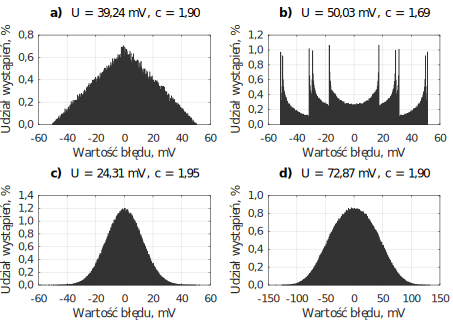
\includegraphics{obrazki/hist_part_S}
\makecaption{fig:symul_partd_hist_S_2_0}{Histogramy błędu \textbf{a)}~statycznego, \textbf{b)}~dynamicznego, \textbf{c)}~losowego, \textbf{d)}~wypadkowego, wielkości wyjściowej $S_{2,0}$ analizowanego w eksperymencie symulacyjnym toru pomiarowego}
\end{center}
\end{figure}

Na podstawie histogramów przedstawionych na rysunkach~\ref{fig:symul_partd_hist_S_2_0} oraz~\ref{fig:symul_partc_hist_T_1_0} zauważyć można, że oszacowane w równaniach od~\eqref{eq:sym_partd_output_unc_roun_S_2_0} do~\eqref{eq:sym_partd_output_unc_dyn_3_S_2_0} oraz od~\eqref{eq:sym_partd_output_unc_roun_T_1_0} do~\eqref{eq:sym_partd_output_unc_dyn_3_T_1_0} parametry sygnałów błędów pokrywają się z tymi uzyskanymi symulacyjnie. Współczynnik $A_{T_{1,0},s} $ określony w równaniu~\eqref{eq:sym_partd_output_as_T_1_0} wskazujący relacje pomiędzy wejściową i wyjściową wariancją błędów statycznych w przypadku wielkości wyjściowej $T_{1,0}$ jest w przybliżeniu równy zero. W rzeczywistości natomiast, ze względu na niewymierność kolejnych współczynników wiersza macierzy transformacji powiązanych z analizowaną wielkością wyjściową, współczynnik ten jest niezerowy. Fakt ten zauważyć można na podstawie rysunku~\ref{fig:symul_partc_hist_T_1_0}, gdzie teoretycznie wszystkie realizacje błędu statycznego powinny być zerowe. Omawiana rozbieżność jest jednak bardzo niewielka i nie wpływa zupełnie na uzyskane wyniki obliczeń.

\begin{figure}[htb!]
\begin{center}
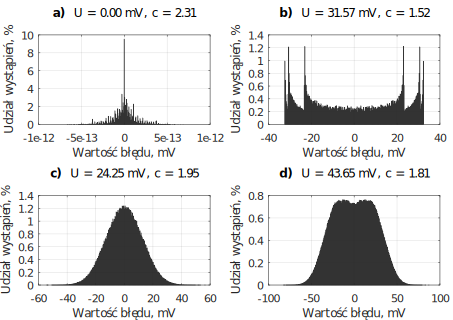
\includegraphics{obrazki/hist_part_T}
\makecaption{fig:symul_partc_hist_T_1_0}{Histogramy błędu \textbf{a)}~statycznego, \textbf{b)}~dynamicznego, \textbf{c)}~losowego, \textbf{d)}~wypadkowego, wielkości wyjściowej $T_{1,0}$ analizowanego w eksperymencie symulacyjnym toru pomiarowego uzyskane metodą Monte-Carlo}
\end{center}
\end{figure}

Wobec powyższych informacji wnioskować można, że przeprowadzony eksperyment wykazał poprawność zaproponowanej metody analizy oraz stworzonego na potrzeby pracy modelu błędu. Oszacowana przy użyciu proponowanej metody wartość wariancji dla analizowanych źródeł błędów oraz dla błędów wypadkowych każdorazowo okazywała się zbieżna z wartością uzyskaną metodą symulacyjną. Uzyskane wartości niepewności rozszerzonej, wyznaczane z użyciem redukcyjnej arytmetyki interwałowej, cechowały się rozbieżnością na poziomie mniejszym niż $<-5;5> \%$, a zatem również uznać można je za poprawne. Eksperyment wykazał możliwość stosowania uproszczenia obliczeń, które wynika bezpośrednio z warunków centralnego twierdzenia granicznego, natomiast stosowanie go dopuszczone jest tylko i wyłącznie w określonych warunkach. Stosowanie założeń centralnego twierdzenia granicznego w przypadkach o niewielkiej liczbie niezależnych źródeł błędów lub w przypadkach istnienia dominującego źródła błędu skutkować będzie przekraczającym $5\%$ błędem oszacowania niepewności rozszerzonej, co w wielu przypadkach może być uznawane za niedopuszczalne.

Zgodnie z założeniami przedstawionymi we wstępie podrozdziału, ostatnią czynnością weryfikującą symulacyjnie poprawność przedstawionych w pracy założeń będzie przeprowadzenie powyższej analizy wykorzystując budżet niepewności zestawiony w tabeli~\ref{tab:sym_partc_params_unc_list}. Jako, że wyznaczanie parametrów kolejnych składowych sygnałów błędów odbywać się będzie analogicznie, jak miało to miejsce w przykładach opisanych zależnościami od~\eqref{eq:sym_partd_output_var_stat_S_2_0} do~\eqref{eq:sym_partd_output_var_dyn_3_S_2_0} oraz od~\eqref{eq:sym_partd_output_unc_stat_S_2_0} do~\eqref{eq:sym_partd_output_unc_dyn_3_S_2_0}, omawiane wyprowadzenia i obliczenia nie będą przedstawiane. W tabeli~\ref{tab:sym_partd_params_unc_list_S_2_0} zestawiono obliczone parametry wszystkich źródeł błędów wielkości wyjściowej $S_{2,0}$, natomiast parametry wielkości wyjściowej $T_{1,0}$ zestawiono w tabeli~\ref{tab:sym_partd_params_unc_list_T_1_0}.

\begin{table}[htb!]
\begin{center}
\makecaption{tab:sym_partd_params_unc_list_S_2_0}{Budżet niepewności wielkości wyjściowej $S_{2,0}$ analizowanego w eksperymencie symulacyjnym toru pomiarowego, gdzie (a) oznacza przetwornik pomiarowy, (b) oznacza wzmacniacz pomiarowy oraz (c) oznacza przetwornik analogowo-cyfrowy}
\begin{tabular}[c]{| c | c | S[table-format = 2.2] | S[table-format = 3.2] | c | c |} \hline
\textbf{Lp.} & \textbf{Symbol} & \textbf{$U_{95\%}$, mV} & \textbf{$\sigma^{2}$, \micro V} & \textbf{Rozkład} & \textbf{Źródło błędu} \\ \hline
1  & ${rw,z}$     & 2.13  &   0.97  & zaokrągleń                   & operacje zmiennoprzecinkowe                \\ \hline
2  & ${rp,q}$     & 13.26 &  45.78  & normalny                     & proces kwantowania (c)                     \\ \hline
3  & ${rp,1}$     & 11.80 &  36.26  & normalny                     & nieliniowość obiektu (a)                   \\ \hline
4  & ${rp,2}$     & 16.70 &  72.64  & normalny                     & szum wielkości wejściowej                  \\ \hline
5  & ${sp,1}$     & 23.04 &  147.00 & trójkątny                    & dryf temperatury (a)                       \\ \hline
6  & ${sp,2}$     & 16.29 &  73.52  & trójkątny                    & dryf temperatury (b)                       \\ \hline
7  & ${dp,a,1}$   & 12.32 &  76.40  & \multirow{6}{*}{dwumodalny}  & \multirow{3}{*}{transmitancja (a)}         \\ \cline{1-4}
8  & ${dp,a,2}$   & 25.08 &  316.38 &                              &                                            \\ \cline{1-4}
9  & ${dp,a,3}$   & 2.35  &  2.77   &                              &                                            \\ \cline{1-4} \cline{6-6}
10 & ${dp,b,1}$   & 6.07  &  18.52  &                              & \multirow{3}{*}{transmitancja (b)}         \\ \cline{1-4}
11 & ${dp,b,2}$   & 12.35 &  76.70  &                              &                                            \\ \cline{1-4}
12 & ${dp,b,3}$   & 1.16  &  0.67   &                              &                                            \\ \hline
\end{tabular}
\end{center}
\end{table}

\begin{table}[htb!]
\begin{center}
\makecaption{tab:sym_partd_params_unc_list_T_1_0}{Budżet niepewności wielkości wyjściowej $T_{1,0}$ analizowanego w eksperymencie symulacyjnym toru pomiarowego, gdzie (a) oznacza przetwornik pomiarowy, (b) oznacza wzmacniacz pomiarowy oraz (c) oznacza przetwornik analogowo-cyfrowy}
\begin{tabular}[c]{| c | c | S[table-format = 2.2] | S[table-format = 3.2] | c | c |} \hline
\textbf{Lp.} & \textbf{Symbol} & \textbf{$U_{95\%}$, mV} & \textbf{$\sigma^{2}$, \micro V} & \textbf{Rozkład} & \textbf{Źródło błędu} \\ \hline
1  & ${rw,z}$     & 1.81  &  0.70   & zaokrągleń                   & operacje zmiennoprzecinkowe                \\ \hline
2  & ${rp,q}$     & 13.26 &  45.78  & normalny                     & proces kwantowania (c)                     \\ \hline
3  & ${rp,1}$     & 11.80 &  36.26  & normalny                     & nieliniowość obiektu (a)                   \\ \hline
4  & ${rp,2}$     & 16.71 &  72.64  & normalny                     & szum wielkości wejściowej                  \\ \hline
5  & ${sp,1}$     & 0.00  &  0.00   & trójkątny                    & dryf temperatury (a)                       \\ \hline
6  & ${sp,2}$     & 0.00  &  0.00   & trójkątny                    & dryf temperatury (b)                       \\ \hline
7  & ${dp,a,1}$   & 0.06  &  0.00   & \multirow{6}{*}{dwumodalny}  & \multirow{3}{*}{transmitancja (a)}         \\ \cline{1-4}
8  & ${dp,a,2}$   & 3.77  &  7.13   &                              &                                            \\ \cline{1-4}
9  & ${dp,a,3}$   & 19.16 &  184.65 &                              &                                            \\ \cline{1-4} \cline{6-6}
10 & ${dp,b,1}$   & 0.03  &  0.00   &                              & \multirow{3}{*}{transmitancja (b)}         \\ \cline{1-4}
11 & ${dp,b,2}$   & 1.85  &  1.73   &                              &                                            \\ \cline{1-4}
12 & ${dp,b,3}$   & 9.44  &  44.82  &                              &                                            \\ \hline
\end{tabular}
\end{center}
\end{table}

Jako, że analiza kolejnych fragmentów toru pomiarowego wykazała korelacje pomiędzy wybranymi sygnałami błędów, wyznaczenie wariancji wypadkowych sygnałów błędów przeprowadzane będzie zgodnie z zależnością~\eqref{eq:alg_outvar_mat}. W dalszej części rozważań przyjmuje się, że symbolem $\bsigma_{*}$ oznaczono wektory złożone z kolejnych odchyleń standardowych sygnałów błędów wielkości wyjściowych algorytmu, przy czym \enquote{$*$} oznacza symbol analizowanej wielkości wyjściowej. Z uwagi na fakt, że analizowany algorytm nie wpływa na istniejące korelacje przetwarzanych sygnałów błędu, macierz korelacji oznaczona symbolem $\mathbf{r}_{d}$ będzie jednakowa dla wszystkich wielkości wyjściowych tego algorytmu i składać się będzie z dwunastu wierszy i kolumn. Zgodnie z równaniem~\eqref{eq:alg_outvar_mat} wartość wariancji wypadkowego sygnału błędu błędu dla wybranej wielkości wyjściowej opisać można w rozważanym przypadku jako:
\begin{equation}
\sigma_{*,\Sigma}^{2} = \bsigma_{*}^{T} \cdot \mathbf{r}_{d} \cdot \bsigma_{*} \label{eq:sym_partd_output_varmat_list}.
\end{equation}
Na podstawie równania~\eqref{eq:sym_partb_stat_corr} korelacja pomiędzy błędami statycznymi wzmacniacza i przetwornika pomiarowego wyniesie $1$, zatem $r_{d,sp,1,2} = 1$. Dodatkowo współczynniki korelacji kolejnych harmonicznych błędu dynamicznego o tej samej częstotliwości są w przybliżeniu równe jedności, a zatem $r_{d,dp,a,b,n} = 1$ dla $n \in \{ 1, 2, 3 \}$. Wobec powyższych macierz korelacji $\mathbf{r}_{d}$ przyjmuje postać:
\begin{equation}
\mathbf{r}_{d} =
\begin{bmatrix}
1.0 & 0.0 & 0.0 & 0.0 & 0.0 & 0.0 & 0.0 & 0.0 & 0.0 & 0.0 & 0.0 & 0.0 \\
0.0 & 1.0 & 0.0 & 0.0 & 0.0 & 0.0 & 0.0 & 0.0 & 0.0 & 0.0 & 0.0 & 0.0 \\
0.0 & 0.0 & 1.0 & 0.0 & 0.0 & 0.0 & 0.0 & 0.0 & 0.0 & 0.0 & 0.0 & 0.0 \\
0.0 & 0.0 & 0.0 & 1.0 & 0.0 & 0.0 & 0.0 & 0.0 & 0.0 & 0.0 & 0.0 & 0.0 \\
0.0 & 0.0 & 0.0 & 0.0 & 1.0 & 1.0 & 0.0 & 0.0 & 0.0 & 0.0 & 0.0 & 0.0 \\
0.0 & 0.0 & 0.0 & 0.0 & 1.0 & 1.0 & 0.0 & 0.0 & 0.0 & 0.0 & 0.0 & 0.0 \\
0.0 & 0.0 & 0.0 & 0.0 & 0.0 & 0.0 & 1.0 & 0.0 & 0.0 & 1.0 & 0.0 & 0.0 \\
0.0 & 0.0 & 0.0 & 0.0 & 0.0 & 0.0 & 0.0 & 1.0 & 0.0 & 0.0 & 1.0 & 0.0 \\
0.0 & 0.0 & 0.0 & 0.0 & 0.0 & 0.0 & 0.0 & 0.0 & 1.0 & 0.0 & 0.0 & 1.0 \\
0.0 & 0.0 & 0.0 & 0.0 & 0.0 & 0.0 & 1.0 & 0.0 & 0.0 & 1.0 & 0.0 & 0.0 \\
0.0 & 0.0 & 0.0 & 0.0 & 0.0 & 0.0 & 0.0 & 1.0 & 0.0 & 0.0 & 1.0 & 0.0 \\
0.0 & 0.0 & 0.0 & 0.0 & 0.0 & 0.0 & 0.0 & 0.0 & 1.0 & 0.0 & 0.0 & 1.0
\end{bmatrix}
\label{eq:sym_partd_output_coher_list}.
\end{equation}

Zgodnie z zależnościami~\eqref{eq:sym_partd_output_varmat_list} oraz~\eqref{eq:sym_partd_output_coher_list}, po podstawieniu danych z tabel~\ref{tab:sym_partd_params_unc_list_S_2_0} oraz~\ref{tab:sym_partd_params_unc_list_T_1_0}, otrzymuje się wartości wariancji wypadkowych sygnałów błędów wielkości wyjściowych $S_{2,0}$ oraz $T_{1,0}$, przy czym kolejno:
\begin{gather}
\sigma_{S_{2,0},\Sigma}^{2} = \bsigma_{S_{2,0}}^{T} \cdot \mathbf{r}_{d} \cdot \bsigma_{S_{2,0}} = \qty{1464.79}{\micro V} \label{eq:sym_partd_output_varmat_S_2_0}, \\
\sigma_{T_{1,0},\Sigma}^{2} = \bsigma_{T_{1,0}}^{T} \cdot \mathbf{r}_{d} \cdot \bsigma_{T_{1,0}} = \qty{582.68}{\micro V} \label{eq:sym_partd_output_varmat_T_1_0}.
\end{gather}
Można zauważyć, że wyznaczone w ten sposób wartości są identyczne, jak te wyznaczone wcześniej w równaniach~\eqref{eq:sym_partd_output_var_sum_S_2_0} oraz~\eqref{eq:sym_partd_output_var_sum_T_1_0}.

Oszacowanie wypadkowej wartości niepewności rozszerzonej kolejnych wielkości wyjściowych odbywać się będzie z wykorzystaniem równania~\eqref{eq:alg_outunc_mat}, przy czym w celu dodatkowej weryfikacji wpływu korekty wartości współczynników koherencji, zaproponowanej w pracy i danej równaniem~\eqref{eq:unc_cohercorra}, obliczenia zostaną wykonane zarówno uwzględniając jak i pomijając tą korektę. Z uwagi na występowanie korelacji pomiędzy analizowanymi sygnałami błędów bezpośrednie zastosowanie metody opisanej równaniem~\eqref{eq:unc_matrix} dla współczynników koherencji wyznaczanych zgodnie z równaniem~\eqref{eq:unc_coher} nie jest możliwe. Proponuje się zatem wyprowadzenie zależności opisujących wypadkowe parametry niepewności rozszerzonej dla grup wzajemnie skorelowanych sygnałów, a następnie zastosowanie tych wartości w równaniu~\eqref{eq:unc_matrix} gdzie nie wystąpią korelacje.

Dla sygnałów błędów statycznych wzmacniacza i przetwornika pomiarowego zapisać można następującą zależność, która określa wypadkową wartość niepewności rozszerzonej analizowanej pary sygnałów:
\begin{equation}
U_{*,sp} = \sqrt{
\begin{bmatrix}
U_{*,sp,1} \\ U_{*,sp,2}
\end{bmatrix}^{T}
\begin{bmatrix}
1 & h_{d,sp,1,2} \\
h_{d,sp,2,1} & 1
\end{bmatrix}
\begin{bmatrix}
U_{*,sp,1} \\ U_{*,sp,2}
\end{bmatrix}}
\label{eq:sym_partd_output_static_corrunc},
\end{equation}
przy czym w przypadku pełnej dodatniej korelacji (tj. dla $r_{d,sp,1,2} = 1$) wartość współczynnika koherencji $h_{d,sp,1,2}$ jest równa $1$. Podobną zależność opisać można dla kolejnych par skorelowanych sygnałów błędów dynamicznych:
\begin{equation}
U_{*,dp,n} = \sqrt{
\begin{bmatrix}
U_{*,dp,a,n} \\ U_{*,dp,b,n}
\end{bmatrix}^{T}
\begin{bmatrix}
1 & h_{d,dp,a,b,n} \\
h_{d,dp,x,2,1} & 1
\end{bmatrix}
\begin{bmatrix}
U_{*,dp,a,n} \\ U_{*,dp,b,n}
\end{bmatrix}}
\label{eq:sym_partd_output_dynamic_corrunc},
\end{equation}
gdzie ze względu na pełną dodatnią korelację zachodzi $h_{d,dp,x,1,2} = 1$. W analizowanych przypadkach, opisanych równaniami~\eqref{eq:sym_partd_output_static_corrunc} oraz~\eqref{eq:sym_partd_output_dynamic_corrunc}, zauważyć można, że wypadkowe sygnały błędów cechować się będą identycznymi kształtami rozkładu, jak ich składowe. Sytuacja ta sprzyja stosowaniu w dalszej części rozważań zależności~\eqref{eq:unc_coher}, jako że istnieje możliwość wykorzystania współczynników kształtu, których wartości dla typowych par rozkładów przedstawiono wcześniej w tabeli~\ref{tab:unc_shapefac}.

Wobec powyższych, wektor niepewności rozszerzonych kolejnych sygnałów błędów dla wielkości wyjściowych analizowanego toru pomiarowego przedstawić można jako:
\begin{equation}
\mathbf{U}_{*} =
\begin{bmatrix}
U_{*,rw,z} & U_{*,rp,q} & U_{*,rp,1} & U_{*,rp,2} & U_{*,sp} & U_{*,dp,1} & U_{*,dp,2} & U_{*,dp,3}
\end{bmatrix}
\label{eq:sym_partd_output_unc_sumuvect},
\end{equation}
natomiast macierze koherencji kolejnych wielkości wyjściowych, których wartości wyznaczane są zgodnie z równaniem~\eqref{eq:unc_coher}, opisać można w postaci:
\begin{equation}
\mathbf{h}_{*} =
\begin{bmatrix}
1 & h_{*,0,1} & h_{*,0,2} & h_{*,0,3} & h_{*,0,4} & h_{*,0,5} & h_{*,0,6} & h_{*,0,7} \\
h_{*,1,0} & 1 & h_{*,1,2} & h_{*,1,3} & h_{*,1,4} & h_{*,1,5} & h_{*,1,6} & h_{*,1,7} \\
h_{*,2,0} & h_{*,2,1} & 1 & h_{*,2,3} & h_{*,2,4} & h_{*,2,5} & h_{*,2,6} & h_{*,2,7} \\
h_{*,3,0} & h_{*,3,1} & h_{*,3,2} & 1 & h_{*,3,4} & h_{*,3,5} & h_{*,3,6} & h_{*,3,7} \\
h_{*,4,0} & h_{*,4,1} & h_{*,4,2} & h_{*,4,3} & 1 & h_{*,4,5} & h_{*,4,6} & h_{*,4,7} \\
h_{*,5,0} & h_{*,5,1} & h_{*,5,2} & h_{*,5,3} & h_{*,5,4} & 1 & h_{*,5,6} & h_{*,5,7} \\
h_{*,6,0} & h_{*,6,1} & h_{*,6,2} & h_{*,6,3} & h_{*,6,4} & h_{*,6,5} & 1 & h_{*,6,7} \\
h_{*,7,0} & h_{*,7,1} & h_{*,7,2} & h_{*,7,3} & h_{*,7,4} & h_{*,7,5} & h_{*,7,6} & 1
\end{bmatrix}
\label{eq:sym_partd_output_unc_cohermat},
\end{equation}
przy czym kolejne indeksy przy współczynnikach macierzy odpowiadają oznaczeniom przyjętym w wektorze niepewności rozszerzonych opisanym równaniem~\eqref{eq:sym_partd_output_unc_sumuvect}, gdzie przykładowo $h_{*,0,1} = h_{*,rw,z,rp,q}$. Wartość wypadkowej niepewności rozszerzonej może być w analizowanym przypadku oszacowana zgodnie z równaniem~\eqref{eq:alg_outunc_mat} jako:
\begin{equation}
U_{*} = \sqrt{\mathbf{U}_{*} \cdot \mathbf{h}_{*} \cdot \mathbf{U}_{*}^{T}} \label{eq:sym_partd_output_unc_totalmat},
\end{equation}

Podstawiając do równania~\eqref{eq:sym_partd_output_static_corrunc} wartości z tabel~\ref{tab:sym_partd_params_unc_list_S_2_0} oraz~\ref{tab:sym_partd_params_unc_list_T_1_0} otrzymuje się wypadkowe wartości niepewności rozszerzonej dla sygnałów wypadkowych skorelowanych błędów statycznych wielkości $S_{2,0}$ oraz $T_{1,0}$ w postaci:
\begin{gather}
\begin{split}
U_{S_{2,0},sp} = & \sqrt{
\begin{bmatrix}
U_{S_{2,0},sp,1} \\ U_{S_{2,0},sp,2}
\end{bmatrix}^{T}
\begin{bmatrix}
1 & h_{d,sp,1,2} \\
h_{d,sp,2,1} & 1
\end{bmatrix}
\begin{bmatrix}
U_{S_{2,0},sp,1} \\ U_{S_{2,0},sp,2}
\end{bmatrix}} = \\ & \sqrt{
\begin{bmatrix}
\num{23.04e-3} \\ \num{16.29e-3}
\end{bmatrix}^{T}
\begin{bmatrix}
1 & 1 \\
1 & 1
\end{bmatrix}
\begin{bmatrix}
\num{23.04e-3} \\ \num{16.29e-3}
\end{bmatrix}} = \qty{39.31}{mV}
\end{split}
\label{eq:sym_partd_output_static_corrunc_S_2_0}, \\
\begin{split}
U_{T_{1,0},sp} = & \sqrt{
\begin{bmatrix}
U_{T_{1,0},sp,1} \\ U_{T_{1,0},sp,2}
\end{bmatrix}^{T}
\begin{bmatrix}
1 & h_{d,sp,1,2} \\
h_{d,sp,2,1} & 1
\end{bmatrix}
\begin{bmatrix}
U_{T_{1,0},sp,1} \\ U_{T_{1,0},sp,2}
\end{bmatrix}} = \\ & \sqrt{
\begin{bmatrix}
0.00 \\ 0.00
\end{bmatrix}^{T}
\begin{bmatrix}
1 & 1 \\
1 & 1
\end{bmatrix}
\begin{bmatrix}
0.00 \\ 0.00
\end{bmatrix}} = \qty{0.00}{mV}
\end{split}
\label{eq:sym_partd_output_static_corrunc__T_1_0},
\end{gather}
natomiast w przypadku równania~\eqref{eq:sym_partd_output_dynamic_corrunc} dla pierwszej harmonicznej sygnałów błędów dynamicznych omawianych wielkości zachodzi:
\begin{gather}
\begin{split}
U_{S_{2,0},dp,1} = & \sqrt{
\begin{bmatrix}
U_{S_{2,0},dp,a,1} \\ U_{S_{2,0},dp,b,1}
\end{bmatrix}^{T}
\begin{bmatrix}
1 & h_{d,dp,a,b,1} \\
h_{d,dp,b,a,1} & 1
\end{bmatrix}
\begin{bmatrix}
U_{S_{2,0},dp,a,1} \\ U_{S_{2,0},dp,b,1}
\end{bmatrix}} = \\ & \sqrt{
\begin{bmatrix}
\num{12.32e-3} \\ \num{6.07e-3}
\end{bmatrix}^{T}
\begin{bmatrix}
1 & 1 \\
1 & 1
\end{bmatrix}
\begin{bmatrix}
\num{12.32e-3} \\ \num{6.07e-3}
\end{bmatrix}} = \qty{18.39}{mV}
\end{split}
\label{eq:sym_partd_output_dynamic_corrunc_S_2_0}, \\
\begin{split}
U_{T_{1,0},dp,1} = & \sqrt{
\begin{bmatrix}
U_{T_{1,0},dp,a,1} \\ U_{T_{1,0},dp,b,1}
\end{bmatrix}^{T}
\begin{bmatrix}
1 & h_{d,dp,a,b,1} \\
h_{d,dp,b,a,1} & 1
\end{bmatrix}
\begin{bmatrix}
U_{T_{1,0},dp,a,1} \\ U_{T_{1,0},dp,b,1}
\end{bmatrix}} = \\ & \sqrt{
\begin{bmatrix}
\num{0.06e-3} \\ \num{0.03e-3}
\end{bmatrix}^{T}
\begin{bmatrix}
1 & 1 \\
1 & 1
\end{bmatrix}
\begin{bmatrix}
\num{0.06e-3} \\ \num{0.03e-3}
\end{bmatrix}} = \qty{0.092}{mV}
\end{split}
\label{eq:sym_partd_output_dynamic_corrunc_T_1_0}.
\end{gather}
Parametry pozostałych harmonicznych sygnałów błędów dynamicznych wyznaczane są w analogiczny sposób, zatem obliczenia z nimi związane nie będą przedstawiane. Po podstawieniu uzyskanych wyników do równania~\eqref{eq:sym_partd_output_unc_sumuvect} otrzymuje się wektory składowych niepewności rozszerzonych dla analizowanych wielkości wyjściowych:
\begin{gather}
\mathbf{U}_{S_{2,0}} =
\begin{bmatrix}
2.13 & 13.26 & 11.80 & 16.71 & 39.33 & 18.39 & 37.42 & 3.50
\end{bmatrix} \cdot \num{e-3}
\label{eq:sym_partd_output_unc_sumuvect_S_2_0_b}, \\
\mathbf{U}_{T_{1,0}} =
\begin{bmatrix}
1.81 & 13.26 & 11.80 & 16.71 & 0.00 & 0.092 & 5.62 & 28.60
\end{bmatrix} \cdot \num{e-3}
\label{eq:sym_partd_output_unc_sumuvect_T_1_0_b},
\end{gather}
przy czym macierze koherencji dla analizowanych wielkości wyjściowych przyjmują wartości zgodnie z równaniem~\eqref{eq:unc_coher}, a zatem:
\begin{gather}
\mathbf{h}_{S_{2,0}} =
\begin{bmatrix}
1 & h_{*,0,1} & h_{*,0,2} & h_{*,0,3} & h_{*,0,4} & h_{*,0,5} & h_{*,0,6} & h_{*,0,7} \\
h_{*,1,0} & 1 & h_{*,1,2} & h_{*,1,3} & h_{*,1,4} & h_{*,1,5} & h_{*,1,6} & h_{*,1,7} \\
h_{*,2,0} & h_{*,2,1} & 1 & h_{*,2,3} & h_{*,2,4} & h_{*,2,5} & h_{*,2,6} & h_{*,2,7} \\
h_{*,3,0} & h_{*,3,1} & h_{*,3,2} & 1 & h_{*,3,4} & h_{*,3,5} & h_{*,3,6} & h_{*,3,7} \\
h_{*,4,0} & h_{*,4,1} & h_{*,4,2} & h_{*,4,3} & 1 & h_{*,4,5} & h_{*,4,6} & h_{*,4,7} \\
h_{*,5,0} & h_{*,5,1} & h_{*,5,2} & h_{*,5,3} & h_{*,5,4} & 1 & h_{*,5,6} & h_{*,5,7} \\
h_{*,6,0} & h_{*,6,1} & h_{*,6,2} & h_{*,6,3} & h_{*,6,4} & h_{*,6,5} & 1 & h_{*,6,7} \\
h_{*,7,0} & h_{*,7,1} & h_{*,7,2} & h_{*,7,3} & h_{*,7,4} & h_{*,7,5} & h_{*,7,6} & 1
\end{bmatrix}
\label{eq:sym_partd_output_unc_cohermat_S_2_0_b}, \\
\mathbf{h}_{T_{1,0}} =
\begin{bmatrix}
1 & h_{*,0,1} & h_{*,0,2} & h_{*,0,3} & h_{*,0,4} & h_{*,0,5} & h_{*,0,6} & h_{*,0,7} \\
h_{*,1,0} & 1 & h_{*,1,2} & h_{*,1,3} & h_{*,1,4} & h_{*,1,5} & h_{*,1,6} & h_{*,1,7} \\
h_{*,2,0} & h_{*,2,1} & 1 & h_{*,2,3} & h_{*,2,4} & h_{*,2,5} & h_{*,2,6} & h_{*,2,7} \\
h_{*,3,0} & h_{*,3,1} & h_{*,3,2} & 1 & h_{*,3,4} & h_{*,3,5} & h_{*,3,6} & h_{*,3,7} \\
h_{*,4,0} & h_{*,4,1} & h_{*,4,2} & h_{*,4,3} & 1 & h_{*,4,5} & h_{*,4,6} & h_{*,4,7} \\
h_{*,5,0} & h_{*,5,1} & h_{*,5,2} & h_{*,5,3} & h_{*,5,4} & 1 & h_{*,5,6} & h_{*,5,7} \\
h_{*,6,0} & h_{*,6,1} & h_{*,6,2} & h_{*,6,3} & h_{*,6,4} & h_{*,6,5} & 1 & h_{*,6,7} \\
h_{*,7,0} & h_{*,7,1} & h_{*,7,2} & h_{*,7,3} & h_{*,7,4} & h_{*,7,5} & h_{*,7,6} & 1
\end{bmatrix}
\label{eq:sym_partd_output_unc_cohermat_T_1_0_b}.
\end{gather}
Po podstawieniu powyższych wartości do równania~\eqref{eq:sym_partd_output_unc_totalmat} otrzymuje się wartości wypadkowych niepewności rozszerzonych analizowanych wielkości wyjściowych toru pomiarowego, gdzie kolejno:
\begin{gather}
U_{S_{2,0}} = \sqrt{\mathbf{U}_{S_{2,0}} \cdot \mathbf{h}_{S_{2,0}} \cdot \mathbf{U}_{S_{2,0}}^{T}} = \qty{74.10}{mV} \label{eq:sym_partd_output_unc_totalmat_S_2_0}, \\
U_{T_{1,0}} = \sqrt{\mathbf{U}_{T_{1,0}} \cdot \mathbf{h}_{T_{1,0}} \cdot \mathbf{U}_{T_{1,0}}^{T}} = \qty{43.37}{mV} \label{eq:sym_partd_output_unc_totalmat_T_1_0}.
\end{gather}
Dla macierzy koherencji, których wartości wyznaczone zostały bez uwzględnienia korekty zaproponowanej w równaniu~\eqref{eq:unc_cohercorra}, tj. kiedy w równaniu~\eqref{eq:unc_coher} przyjmuje się $p_{i,j} = 1$ dla dowolnej pary $i$ oraz $j$, otrzymuje się $U_{S_{2,0}} = \qty{77.32}{mV}$ oraz $U_{T_{1,0}} = \qty{46.09}{mV}$.

tabeli~\ref{tab:sym_partd_params_unc_sum_b} zestawiono wyniki dla pozostałych wielkości wyjściowych oraz ich porównanie z tymi uzyskanymi w poprzednim eksperymencie. Symbolem $a$ oznaczono wartości uzyskane przy założeniu normalnego rozkładu sygnału błędu wypadkowego, symbolem $b$ oznaczono wartości uzyskane z wykorzystaniem budżetu niepewności opisanego w tabeli~\ref{tab:sym_partc_params_unc_sum}. Wartości oznaczone symbolem $c$ dotyczą analizy z wykorzystaniem budżetu niepewności opisanego w tabeli~\ref{tab:sym_partc_params_unc_list}, przy czym wielkości oznaczone symbolem $d$ wyznaczono identycznie, jak dla $c$, z tą różnicą że nie stosowano korekty opisanej równaniem~\eqref{eq:unc_cohercorra} w procesie wyznaczania wartości współczynników koherencji. Podobnie, jak w zestawieniu zawartym w tabeli~\ref{tab:sym_partd_params_unc_sum_a}, wielkości oznaczone symbolem $s$ dotyczą przeprowadzonego eksperymentu metodą Monte-Carlo, natomiast symbolem $\delta_{*}$ oznaczono błąd względny oszacowania wartości niepewności rozszerzonej metodą $a$, $b$, $c$ oraz $d$ w odniesieniu do wartości $U_{s}$, wyrażony w procentach.

\begin{table}[htb!]
\begin{center}
\makecaption{tab:sym_partd_params_unc_sum_b}{Porównanie uzyskanych przedstawionymi w pracy metodami wartości wypadkowych niepewności rozszerzonych kolejnych wielkości wyjściowych analizowanego w eksperymencie symulacyjnym toru pomiarowego}
\begin{tabular}[c]{| c | c | c | c | c | c | S[table-format = +1.2] | S[table-format = +1.2] | S[table-format = +1.2] | S[table-format = +1.2] |} \hline
\multirow{2}{*}{\textbf{Wielkość}} & \multicolumn{5}{c|}{\textbf{Niepewność, mV}} & \multicolumn{4}{c|}{\textbf{Błąd, \%}} \\ \cline{2-10}
& $U_{a}$ & $U_{b}$ & $U_{c}$ & $U_{d}$ & $U_{s}$ & $\delta_{a}$ & $\delta_{b}$ & $\delta_{c}$ & $\delta_{d}$ \\ \hline
$S_{2.0}$ & 75.01 & 74.00 & 74.10 & 77.32 & 72.87 & +2.94 & +1.55 & +1.69 & +6.11 \\ \hline
$S_{2.1}$ & 68.19 & 68.44 & 68.43 & 71.52 & 67.09 & +1.64 & +2.01 & +2.00 & +6.60 \\ \hline
$T_{2.0}$ & 57.29 & 56.26 & 55.91 & 57.58 & 53.89 & +6.31 & +4.40 & +3.75 & +6.85 \\ \hline
$T_{2.1}$ & 58.86 & 55.59 & 55.60 & 59.47 & 54.92 & +7.17 & +1.22 & +1.24 & +8.28 \\ \hline
$T_{1.0}$ & 47.31 & 43.61 & 43.37 & 46.09 & 43.76 & +8.11 & -0.34 & -0.89 & +5.32 \\ \hline
$T_{1.1}$ & 47.31 & 43.60 & 43.37 & 46.08 & 43.74 & +8.16 & -0.32 & -0.85 & +5.35 \\ \hline
$T_{1.2}$ & 47.31 & 43.60 & 43.37 & 46.08 & 43.76 & +8.11 & -0.37 & -0.89 & +5.30 \\ \hline
$T_{1.3}$ & 44.79 & 43.64 & 43.39 & 45.43 & 43.17 & +3.75 & +1.09 & +0.51 & +5.24 \\ \hline
\end{tabular}
\end{center}
\end{table}

Analizując wyniki przedstawione w tabeli~\ref{tab:sym_partd_params_unc_sum_b} zauważyć można, że zaproponowana w pracy metoda szacowania wypadkowej wartości niepewności rozszerzonej wraz z zastosowaniem proponowanego modelu błędu zapewniają wyniki zbieżne z tymi uzyskanymi symulacyjnie. Korekta wartości współczynników koherencji opisana równaniem~\eqref{eq:unc_cohercorra} pozwala na znaczne zmniejszenie rozbieżności pomiędzy szacowaną zgodnie z równaniem~\eqref{eq:unc_matrix} wartością, a wartością uzyskiwaną symulacyjnie, w stosunku do wartości uzyskanych bez stosowania opisanej korekty. Wartości uzyskane przy zastosowaniu budżetu niepewności zawierającego jedynie wypadkowe parametry sygnałów błędów z uwzględnieniem na wprowadzone kategorie błędów są zbieżne z wartościami uzyskanymi dla budżetu obejmującego charakterystykę każdego z sygnałów błędów. Rozbieżności pomiędzy wartościami oznaczonymi symbolami $b$ oraz $c$ wynikają z innego oszacowania wartości współczynników koherencji.

\section{Podsumowanie przeprowadzonego eksperymentu}

Przedstawione w bieżącym rozdziale rozważania i przeprowadzone eksperymenty potwierdzają poprawność proponowanego w pracy modelu błędu oraz skuteczność stosowanej metody redukcyjnej arytmetyki interwałowej. Oszacowane zgodnie z równaniem~\eqref{eq:unc_matrix} wartości wypadkowej niepewności rozszerzonej dla współczynników koherencji szacowanych zgodnie z zależnością~\eqref{eq:unc_coher} każdorazowo okazywały się zbieżne z wynikami uzyskiwanymi dla przeprowadzonych metodą Monte-Carlo eksperymentów.

Wartości niepewności oszacowane stosując zaproponowaną w pracy korektę wartości współczynników koherencji daną równaniem~\eqref{eq:unc_cohercorra} były bliższe uzyskanym eksperymentalnie, natomiast w praktyce pomiarowej korekta ta nie jest wymagana, jeżeli dopuszcza się przekraczający $5\%$ błąd oszacowania wartości wypadkowej niepewności rozszerzonej. Należy również brać pod uwagę, że oszacowane w proponowany sposób wartości niepewności rozszerzonej mogą być w pewnych przypadkach nieco niższe, niż wartości prawdziwe. Różnice te nie przekraczają jednak $-3\%$ wartości prawdziwej, co wykazano w eksperymencie, którego wyniki przedstawiono wcześniej na rysunku~\ref{fig:hist_reductive} oraz w przedstawionych dotychczas rozważaniach.

Stosowanie uproszczenia, gdzie zakłada się normalny rozkład błędu wypadkowego, pozwala znacznie uprościć proces wyznaczania wypadkowej wartości niepewności rozszerzonej i zastąpić konieczność stosowania zależności~\eqref{eq:unc_matrix} oraz~\eqref{eq:unc_coher} wyznaczeniem wariancji wypadkowego sygnału błędu, natomiast jego stosowanie wymaga posiadania pewności odnoście spełnienia warunków centralnego twierdzenia granicznego. Jak wykazały przeprowadzone eksperymenty, nawet dla kilkunastu źródeł błędów, gdzie większość z nich nie jest wzajemnie skorelowana, założenie to może okazać się niespełnione, co skutkuje znaczną rozbieżnością pomiędzy oszacowaną, a prawdziwą wartością niepewności rozszerzonej na poziomie zbliżonym do $10\%$.

Jako, że żaden z etapów szacowania wypadkowej wartości niepewności rozszerzonej zgodnie z zaproponowaną metodą nie wymaga przeprowadzania dodatkowych symulacji metodą Monte-Carlo, a wykonywane obliczenia sprowadzają się do prostych operacji arytmetycznych, przedstawiona metoda może zostać zaimplementowana w torze pomiarowym w celu bieżącej oceny jego właściwości metrologicznych. W przypadku zmiany parametrów sygnałów błędów obecnych w analizowanym torze pomiarowym wymagane jest jedynie ponowne wyznaczenie wartości macierzy koherencji i wskazanie parametrów istniejących sygnałów błędów. Istotnymi parametrami analizowanych sygnałów błędów jest w tym przypadku wartość niepewności rozszerzonej dla wybranego, identycznego dla wszystkich wielkości poziomu ufności oraz rodzaj rozkładu analizowanego sygnału.

W przypadku, gdy analizowane sygnały błędów składowych cechować się będą nietypowym rozkładem, stosowanie omawianej w pracy metody wymagać będzie wyznaczenia wartości współczynników kształtu dla wszystkich analizowanych typów rozkładów. Jest to jedyna czynność, której przeprowadzenie nie będzie mogło zwykle odbywać się w czasie pracy systemu pomiarowego i będzie musiała zostać przeprowadzona na etapie identyfikacji jego właściwości. Podobny problem napotkać można w przypadku wystąpienia korelacji pomiędzy analizowanymi sygnałami błędów składowych -- należy wtedy postąpić identycznie, jak pokazano w przykładzie lub zastosować inną metodę wyznaczania wartości elementów macierzy koherencji, jak chociażby pokazano w pracy~\cite{jakubiec_reductive}.

\chapter{Pomiarowa weryfikacja tezy}

Ostatni etap weryfikacji postawionej w pracy tezy stanowi analiza właściwości metrologicznych przykładowego toru pomiarowego, który stworzony został na potrzeby pracy. Analizowany tor pomiarowy przetwarza zmienny w czasie sygnał napięciowy $s(t)$ o chwilowej wartości napięcia z przedziału $\hat{s}(t) \in~<0;1>~\unit{V}$. W celu dopasowania poziomu sygnału napięcia wejściowego do zakresu napięcia wejściowego przetwornika analogowo-cyfrowego oraz zwiększenia impedancji wejściowej toru pomiarowego, sygnał $s(t)$ podawany jest na wejście wzmacniacza pomiarowego. Sygnał wyjściowy $y(t)$ wzmacniacza przetwarzany jest na postać cyfrową $c(i)$, a następnie po wykonaniu odtwarzania statycznego, podawany jest w postaci wielkości $x(i)$ na wejście jednostki \enquote{DSP}, która dla każdego $j$-tego okna pomiarowego pobiera $N$ próbek tego sygnału i wyznacza na ich podstawie $M$ wartości wielkości wyjściowych wektora $\mathbf{X}(j)$, stosując w tym celu algorytm dyskretnej transformacji falkowej. Schemat blokowy omawianego toru pomiarowego przedstawiono na rysunku~\ref{fig:chain_real}.

\begin{figure}[htb!]
\begin{center}
\includegraphics{obrazki/schemat_real}
\makecaption{fig:chain_real}{Schemat blokowy stworzonego na potrzeby pracy toru pomiarowego będącego obiektem przeprowadzanego eksperymentu}
\end{center}
\end{figure}

Do realizacji układu wzmacniacza pomiarowego zastosowany został wzmacniacz operacyjny \enquote{MCP6002}~\cite{microchip_manual} w konfiguracji nieodwracającej, o docelowym wzmocnieniu wynoszącym~\qty{3.3}{V \per V}. Napięcie zasilania wzmacniacza wynosi~\qty{3.3}{V} i pochodzi ze stabilizatora \enquote{LD1117}~\cite{stm_manual} typu \enquote{LDO} (ang. \enquote{Low Dropout}). Zaproponowana konfiguracja, zgodnie z wcześniejszymi założeniami, zapewnia wysoką impedancję wejściową toru pomiarowego oraz bardzo niską impedancję wyjściową wzmacniacza. Parametry statyczne oraz dynamiczne analizowanego obiektu wymagają identyfikacji, ze względu na niedostateczne informacje zawarte w dokumentacji wykorzystanego układu oraz nieznajomości dokładnego modelu dla zastosowanej aplikacji. Należy zauważyć, że dokładna analiza zastosowanego układu byłaby skomplikowana i nie jest konieczna do oceny jego właściwości metrologicznych związanych z zastosowanie proponowanego w pracy modelu błędu.

Zastosowany przetwornik analogowo-cyfrowy stanowi $12$-bitowy przetwornik wagowy~\enquote{SAR} (ang. \enquote{Successive Approximation Register}), wbudowany w mikrokontroler \enquote{STM32F411}~\cite{stm_f411}. Źródło napięcia odniesienia stanowi w jego przypadku stabilizator \enquote{AP7343}~\cite{diodes_manual} typu \enquote{LDO}, o znamionowym napięciu wyjściowym równym~\qty{3.3}{V}, przyłączony z użyciem dodatkowego filtru LC. Przetwornik analogowo-cyfrowy taktowany jest sygnałem zegarowym o częstotliwości~\qty{24}{MHz}, przy czym próbkowanie wyzwalane jest sygnałem z licznika, którego częstotliwość wyzwalania wynosi $f_{s} = \qty{48}{kHz}$. Na pojedynczy proces konwersji analogowo-cyfrowej przypada kluczowanie napięcia wejściowego, trwające $15$ taktów zegara, po którym następuje konwersja, trwająca $15$ taktów zegara, co w analizowanym przypadku stanowi czas~\qty{625}{ns} dla każdej z operacji. Łączny czas konwersji analogowo-cyfrowej pojedynczej próbki sygnału wejściowego $y(t)$ na jego dyskretną reprezentację $c(i)$ wynosi zatem~\qty{1250}{ns}. Ze względu na typową aplikacje omawianego przetwornika, jego najistotniejsze parametry metrologiczne mogą zostać pozyskane z dokumentacji producenta układu~\cite{stm_f411}. Algorytm odtwarzania statycznego przekształca sygnał $c(i)$ na sygnał $x(i)$ tak, aby stanowił on dyskretną reprezentację sygnału $s(t)$ o czułości \qty{1}{V \per V} względem tego sygnału.

Pozyskane próbki napięcia $x(i)$, stanowiące dyskretną reprezentację sygnału wejściowego $s(t)$, zapisywane są w wektorze $\mathbf{x}(j)$ o długości $N = 128$. Wektor wielkości wejściowych $\mathbf{x}(j)$ podawany jest na wejście algorytmu dyskretnej transformacji falkowej, którego implementacja zrealizowana została z wykorzystaniem instrukcji \enquote{DSP} dostępnych dla zastosowanego mikrokontrolera~\cite{reay_dsp}. Analizowany algorytm wykorzystuje falkę \enquote{spline4:4}~\cite{wang_splinebasics} dla pięciu iteracji procesu dekompozycji sygnału. Zgodnie z równaniem~\eqref{eq:alg_out_mat} wyznaczanych jest $M = 128$ próbek wektora wielkości wyjściowych $\mathbf{X}(j)$, które stanowią wyjście dla pojedynczej $j$-tej serii pomiarowej analizowanego toru pomiarowego. Wartości elementów macierzy transformacji $\mathbf{A}$ zidentyfikowano zgodnie z metodą przedstawioną w równaniu~\eqref{eq:wt_ident}, wykorzystując w tym celu implementacje algorytmu transformacji falkowej dostępną w programie \enquote{GNU Octave}~\cite{pruuvsa_dwt}. Czas obliczeń wynosi w analizowanym przypadku~\qty{1508}{\micro s}, przy czym łączny czas akwizycji pojedynczego wektora próbek wielkości wejściowych wynosi~\qty{2666.6(6)}{\micro s}. Podczas obliczeń stosowane są liczby zmiennoprzecinkowe pojedynczej precyzji o długości słowa $32$-bitów, implementowane sprzętowo przez jednostkę \enquote{FPU} (ang. \enquote{Floating Point Unit}~\cite{cortex_fpu, gcc_manual}.

Przedstawiony tor pomiarowy pracuje w trybie ciągłym, tj. w pojedynczym $j$-tym oknie pomiarowym, podczas pobierania próbek wielkości wejściowych wektora $\mathbf{x}(j)$, wyznaczana jest realizacja wektora wielkości wyjściowych $\mathbf{X}(j-1)$ dla poprzedniej realizacji wektora wielkości wejściowych $\mathbf{x}(j-1)$. Wykorzystywany jest w tym celu kontroler \enquote{DMA} (ang. \enquote{Direct Memory Access}), nadzorujący proces buforowania kolejnych realizacji sygnału $x(i)$, w czasie gdy program główny wykonuje obliczenia dane równaniem~\eqref{eq:alg_out_mat}. Analiza wartości wielkości wyjściowych omawianego toru pomiarowego jest możliwa między innymi po podłączeniu go do komputera klasy \enquote{PC} za pośrednictwem portu \enquote{USB}, przy czym wykorzystywany jest w tym celu układ peryferyjny \enquote{USB OTG Full-Speed}, zintegrowany w zastosowanym mikrokontrolerze. Alternatywną możliwość komunikacji z urządzeniem stanowi interfejs \enquote{UART} (ang. \enquote{Universal Asynchronous Receiver-Transmitter}), natomiast ze względu na ograniczenie szybkości transferu danych przez ten interfejs, nie umożliwia on ciągłego śledzenia wyników pomiarów.

W dalszej części rozdziału opisano najważniejsze źródła błędów analizowanego toru pomiarowego, a następnie wykorzystano zaproponowany w pracy model błędu do opisu właściwości wykazanych sygnałów błędów. Ze względu na fakt, że nie jest znany dokładny model analizowanego toru pomiarowego, przeprowadzono identyfikację jego właściwości, istotnych ze względu na zaproponowany model błędu. W ostatniej części rozdziału opisano przeprowadzony eksperyment pomiarowy, wykorzystujący metodę Monte-Carlo, mający na celu ocenę poprawności przedstawionych rozważań i weryfikacje możliwości praktycznej aplikacji zawartych w pracy propozycji. Poza analizą właściwości metrologicznych zbudowanego toru pomiarowego, przeprowadzona analiza obejmowała również wpływ sygnałów błędów zawartych w przetwarzanej wielkości $s(t)$ na budżet niepewności analizowanego urządzenia. Podczas eksperymentów wykorzystano generator przebiegów arbitralnych, którego rzeczywiste parametry sygnału wejściowego w zależności od wariantu eksperymentu weryfikowano, lub pozostawiano nieznane. Celem omawianego zabiegu było przedstawienie przykładu, w jaki sposób stosując zaproponowany w pracy model błędu należy rozpatrywać omawiane rozbieżności w nastawie parametrów syntezowanego sygnału. Temperatura otoczenia podczas przeprowadzania eksperymentów była stała i wynosiła~\qty{21}{\degreeCelsius}.

\section{Model błędu wielkości wejściowej}

Jako, że w analizowanym przypadku źródło napięciowego sygnału wejściowego $s(t)$ toru pomiarowego stanowi generator przebiegów arbitralnych RIGOL DG1011~\cite{rigol_fawg}, należy uwzględnić jego parametry w budżecie niepewności. Zgodnie z dokumentacją, błąd graniczny nastawy wartości amplitudy $E$ sygnału wyjściowego generatora wynosi:
\begin{equation}
\delta_{E,gr} = \pm \emb{\frac{0.5}{100} \left| E \right| + \frac{0.5}{1000}} ~\unit{V} \label{eq:pom_gen_amperr_max},
\end{equation}
natomiast błąd graniczny nastawy składowej stałej $D$ sygnału wyjściowego wynosi:
\begin{equation}
\delta_{D,gr} = \pm \emb{\frac{0.5}{100} \left| D \right| + \frac{2}{1000}} ~\unit{V} \label{eq:pom_gen_shferr_max},
\end{equation}
przy czym omawiane wielkości $E$ oraz $D$ wyrażone są w woltach. Na podstawie powyższych zależności należy oszacować przedział dla zadanego poziomu ufności, w jakim znajduje się $\alpha$ wartości realizacji błędu nastawy amplitudy oraz błędu nastawy składowej stałej. Zgodnie z wytycznymi zawartymi w~\cite{jcgm_guide} i przyjętym w pracy poziomem ufności $\alpha = 95\%$ zapisać można:
\begin{gather}
U_{E} \emb{x} = c_{u} \cdot \sigma_{E} \emb{x} = c_{u} \frac{\left| \delta_{E,gr} \emb{x} \right|}{\sqrt{3}} = 1.65 \frac{\num{5e-3} \left| x \right| + \num{0.5e-3}}{\sqrt{3}} ~\unit{V} \label{eq:pom_gen_amperr_unc}, \\
U_{D} \emb{x} = c_{u} \cdot \sigma_{D} \emb{x} = c_{u} \frac{\left| \delta_{D,gr} \emb{x} \right|}{\sqrt{3}} = 1.65 \frac{\num{5e-3} \left| x \right| + \num{2e-3}}{\sqrt{3}} ~\unit{V} \label{eq:pom_gen_shferr_unc}.
\end{gather}
gdzie $x$ jest wartością zadaną dla analizowanego parametru wyrażoną w woltach. Należy zauważyć, że w przypadku pojedynczego przyrządu, omawiane rozbieżności w nastawie przedstawionych parametrów stanowią systematyczne źródło błędów, a ich wpływ nożna skorygować przeprowadzając kalibrację przyrządu. Niezależnie od wykonania kalibracji przyrządu, dla syntezowanego sygnału sinusoidalnie zmiennego o wartości zadanej amplitudy $\dot{E}_{s,o}$ oraz składowej stałej o wartości zadanej $\dot{D}_{s,o}$, sygnał $s(t)$ na wyjściu przyrządu opisać można w dziedzinie czasu za pomocą równań:
\begin{gather}
\dot{s} \emb{t} = \dot{E}_{s,o} \sin \emb{\omega_{s,o} t} \label{eq:pom_gen_out_ideal}, \\
\tilde{s} \emb{t} = \dot{s} \emb{t} + e_{s,s} \emb{t} + e_{s,d} \emb{t} + e_{s,r} \emb{t}\label{eq:pom_gen_out_real},
\end{gather}
gdzie symbolem $e_{s,s}(t)$ oznaczono błąd statyczny, symbolem $e_{s,s}(t)$ błąd dynamiczny, natomiast symbolem $e_{s,r}(t)$ oznaczono sygnał błędu losowego. Deterministyczna postać sygnałów błędów $e_{s,s}(t)$ oraz $e_{s,d}(t)$ nie jest znana, jeżeli dla konkretnego modelu urządzenia nie zostanie wykonana kalibracja. Jeżeli eksperyment nie zakłada wykonywania kalibracji stosowanego przyrządu, koniczne jest wskazanie opisu przedstawionych sygnałów w kategorii probabilistycznej, przy czym należy wskazać parametry tych sygnałów, których wartość umożliwi wskazanie niepewności rozszerzonej związanej z ich wpływem o zadanym poziomie ufności $\alpha$. Po wykonaniu kalibracji oraz wykonaniu korekty błędów systematycznych można przyjąć, że $e_{s,s}(t) = 0$ oraz $e_{s,d}(t) = 0$. W przypadku, gdy błędy systematyczne nie zostaną skorygowane po wykonaniu kalibracji, należy opisać deterministycznie przebiegi sygnałów związanych z tymi błędami oraz wskazać wartości ich wariancji i niepewności rozszerzonej.

W przypadku sygnału błędu statycznego $e_{s,s}(t)$ przyjąć można, że błąd ten powodowany jest rozbieżnością nastawy wartości składowej stałej. Wartość realizacji tego sygnału jest stała dla zadanej wartości parametru $\dot{D}_{s,o}$, natomiast jego parametry określać może wariancja oraz niepewność rozszerzona, definiowane na podstawie równania~\eqref{eq:pom_gen_amperr_unc}. Zatem, w przypadku braku kalibracji przyrządu zapisać można:
\begin{gather}
e_{s,s} \emb{t} = E_{s,e,0} \emb{\dot{D}_{s,o}} = \tilde{D}_{s,o} - \dot{D}_{s,o} \label{eq:pom_gen_err_stat}, \\
\sigma_{s,s}^{2} = \sigma_{D}^{2} \emb{\dot{D}_{s,o}} = \frac{\left| \delta_{D,gr} \emb{\dot{D}_{s,o}} \right|^{2}}{3} ~\unit{V} \label{eq:pom_gen_var_stat}, \\
U_{s,s} = c_{u} \cdot \sigma_{D} \emb{\dot{D}_{s,o}} = 1.65 \frac{\num{5e-3} \left| \dot{D}_{s,o} \right| + \num{2e-3}}{\sqrt{3}} ~\unit{V} \label{eq:pom_gen_unc_stat}.
\end{gather}
gdzie $\tilde{D}_{s,o}$ jest rzeczywistą wartością składowej stałej dla wartości zadanej równej $\dot{D}_{s,o}$. Po przeprowadzeniu kalibracji istnieje możliwość deterministycznego opisu sygnału $e_{s,s}(t)$ w funkcji zadanej wartości $\dot{D}_{s,o}$, przy czym wartość tego sygnału jest stała w czasie. Po wykonaniu korekty założyć można, że sygnał ten nie występuje, zatem $e_{s,s}(t) = 0$.

Sygnał błędu dynamicznego $e_{s,d}(t)$ wynikać będzie z rozbieżności nastawy amplitudy względem wartości zadanej $\dot{E}_{s,o}$. Sygnał ten opisać można w postaci:
\begin{equation}
e_{s,d} \emb{t} = \emb{\tilde{E}_{s,o} - \dot{E}_{s,o}} \sin \emb{\omega_{s,o} t} = E_{s,e,1} \emb{\dot{E}_{s,o}} \sin \emb{\omega_{s,o} t + \varphi_{s,e,1} \emb{\dot{E}_{s,o}}} \label{eq:pom_gen_err_dyn_mono},
\end{equation}
gdzie $\tilde{E}_{s,o}$ jest rzeczywistą amplitudą, $E_{s,e,1}(\dot{E}_{s,o})$ jest wartością amplitudy oraz $\varphi_{s,e,1}(\dot{E}_{s,o})$ jest fazą sygnału błędu dynamicznego w funkcji zadanej wartości amplitudy $\dot{E}_{s,o}$. Jako, że błąd nastawy amplitudy sygnału może przyjmować zarówno dodatni, jak ujemny znak, należy rozważać sygnał z nim związany dla obydwóch przypadków. Sytuacje te odróżnić należy analizując inną fazę $\varphi_{s,e,1}$ tego sygnału, przy czym dla dodatniej wartości sygnału błędu zachodzi $\varphi_{s,e,1} = 0$, natomiast dla ujemnej $\varphi_{s,e,1} = \pi$. Kalibracja przyrządu prowadzi do zdeterminowania zależności $E_{s,e,1} \emb{\dot{E}_{s,o}}$ i umożliwia korektę opisanego sygnału błędu. Jeżeli po wykonaniu wzorcowania nie uwzględnia się korekty związanej z nastawą amplitudy, to wariancję sygnału błędu $e_{s,d}(t)$ wyznaczyć można zgodnie z zależnością~\eqref{eq:dyn_var}, natomiast w przypadku braku kalibracji, należy określić maksymalną wariancję tego sygnału w postaci:
\begin{equation}
\sigma_{s,d}^{2} = \frac{U_{E}^{2} \emb{\dot{E}_{s,o}}}{2} = \frac{1.65^{2}}{6} \emb{\num{5e-3} \dot{E}_{s,o} + \num{0.5e-3}}^{2} \unit{V} \label{eq:pom_gen_var_dyn},
\end{equation}
która odpowiada wartości błędu granicznego nastawy amplitudy dla $95\%$ przypadków. Należy zauważyć, że wartość amplitudy sygnału błędu dynamicznego $e_{s,d}(t)$ jest stała w czasie i zależy jedynie od wartości parametru $\dot{E}_{s,o}$. Z uwagi na fakt, że bez procedury kalibracji rzeczywista wartość $\tilde{E}_{s,o}$ nie jest znana, należy przyjąć taką wartość wariancji $\sigma_{s,d}^{2}$ sygnału błędu dynamicznego $e_{s,d}(t)$, która z prawdopodobieństwem $95\%$ obejmie wszystkie możliwe przypadki realizacji tego błędu, niezależnie od użytego egzemplarza urządzenia dla zadanej wartości $\dot{E}_{s,o}$.

W przypadku sygnałów poliharmonicznych należy analizować przebieg sygnału błędu dynamicznego analogicznie, jak pokazano w równaniu~\eqref{eq:pom_gen_err_dyn_mono}, przy czym przykładowo dla sygnału trójkątnego zapisać można:
\begin{gather}
\dot{s} \emb{t} = \dot{D}_{s,o} + \dot{E}_{s,o} \frac{\pi}{8} \sum _{i=1} ^{\infty} \emb{-1}^{i-1} \emb{2i - 1}^{-2} \sin \emb{\omega_{s,o} t \emb{2i - 1}} \label{eq:pom_gen_triangle_ideal}, \\
\tilde{s} \emb{t} = \tilde{D}_{s,o} + \tilde{E}_{s,o} \frac{\pi}{8} \sum _{i=1} ^{\infty} \emb{-1}^{i-1} \emb{2i - 1}^{-2} \sin \emb{\omega_{s,o} t \emb{2i - 1}} \label{eq:pom_gen_triangle_real},
\end{gather}
zatem sygnał błędu dynamicznego zdefiniować można w postaci sumy harmonicznych tego sygnału o amplitudzie zależnej od realizacji błędu nastawy amplitudy:
\begin{gather}
e_{s,d} \emb{t} = \sum _{i=1} ^{\infty} E_{s,e,i} \emb{\dot{E}_{s,o}} \sin \emb{\omega_{s,o} t \emb{2i - 1}} \label{eq:pom_gen_err_dyn_triangle}, \\
E_{s,e,i} \emb{\dot{E}_{s,o}} = \frac{\pi}{8} \emb{2i - 1}^{-2} \emb{\tilde{E}_{s,o} - \dot{E}_{s,o}} \label{eq:pom_gen_err_amp_triangle}, \\
\varphi_{s,e,i} = 
\begin{cases}
0   & $dla $ \tilde{E}_{s,o} - \dot{E}_{s,o} > 0 $ oraz $ \emb{-1}^{i-1} =  1 \\
\pi & $dla $ \tilde{E}_{s,o} - \dot{E}_{s,o} > 0 $ oraz $ \emb{-1}^{i-1} = -1 \\
0   & $dla $ \tilde{E}_{s,o} - \dot{E}_{s,o} < 0 $ oraz $ \emb{-1}^{i-1} = -1 \\
\pi & $dla $ \tilde{E}_{s,o} - \dot{E}_{s,o} < 0 $ oraz $ \emb{-1}^{i-1} =  1
\end{cases}
\label{eq:pom_gen_err_phi_triangle}.
\end{gather}
Należy zaznaczyć, że w zależności od znaku błędu nastawy amplitudy zmienia się faza sygnału tego błędu. Niezależnie od znaku, wartość wariancji tego sygnału pozostaje niezmienna, natomiast znak ten jest istotny z punktu widzenia rozpatrywania korelacji sygnału błędu dynamicznego generatora $e_{s,d}(t)$ oraz pozostałych sygnałów błędów dynamicznych. Jako, że bez zabiegu wzorcowania przyrządu nie ma możliwości determinacji znaku omawianego błędu, należy rozważyć w ostatecznej ocenie mniej korzystną opcję, tj. tą, o większej wartości wariancji wypadkowego sygnału błędu.

Ostatnim analizowanym sygnałem jest sygnał błędu losowego $e_{s,r}(t)$, na który składają się między innymi błąd kwantowania związany z rozdzielczością przetwornika cyfrowo-analogowego oraz szum zawarty w sygnale wyjściowym. Dokumentacja urządzenia nie pozwala na precyzyjne określenie wariancji szumu obecnego w sygnale wyjściowym z uwagi na brak danych odnośnie tego zjawiska. Mimo, że dokumentacja układu wskazuje rozdzielczość przetwornika cyfrowo-analogowego równą $14$-bitów, to nie wskazuje ona kolejnych wartości napięcia referencyjnego tego przetwornika dla wybranych wartości amplitudy i składowej stałej sygnału. Bez procedury kalibracyjnej oszacowanie wariancji $\sigma_{s,r}^{2}$ sygnału błędu losowego $e_{s,r}(t)$ jest niemożliwe, zatem przyjmuje się, że $e_{s,r}(t) = 0$ i pomija ten sygnał w dalszej analizie.

Zgodnie z dokumentacją urządzenia błąd graniczny nastawy częstotliwości po roku wynosi maksymalnie \qty{20}{ppm}, natomiast współczynnik temperaturowy tej nastawy w przedziale $\hat{\vartheta} \in~<18;28>\unit{\degreeCelsius}$ nie przekracza \qty{2}{ppm}. Wobec przedstawionych danych nie rozważa się wpływu błędu związanego z nastawą parametru pulsacji $\omega_{s,o}$ na proces wyznaczania wartości wielkości wyjściowych analizowanego toru pomiarowego.

\section{Identyfikacja właściwości toru pomiarowego}

Aplikacja zaproponowanego w pracy modelu błędu wymaga identyfikacji parametrów tego modelu, właściwych dla analizowanego toru pomiarowego. Pierwszą grupą identyfikowanych właściwości analizowanego toru pomiarowego stanowią jego właściwości statyczne. Właściwości te nie zależą od częstotliwości przetwarzanego sygnału i wynikają z charakterystyk przetwarzania statycznego kolejnych fragmentów tego toru. Jako, że z punktu widzenia zaproponowanego w pracy modelu błędu i sposobu jego aplikacji, najistotniejsze informacje stanowią dane dotyczące parametrów sygnałów błędów na wejściu algorytmu dyskretnej transformacji falkowej, najbardziej przystępne z punktu widzenia projektanta toru pomiarowego jest wyznaczenie tych parametrów traktując całość toru pomiarowego znajdującego się przed tym algorytmem, jak jeden obiekt o wypadkowych parametrach wszystkich pozostałych fragmentów tego toru.

Wobec powyższych, proponuje się wyznaczenie charakterystyki statycznej $f_{c}(x)$ dla wielkości wyjściowej $c(i)$ przetwornika analogowo-cyfrowego, a następnie na jej podstawie określenie funkcji odtwarzania $f_{x}(x)$. Należy w tym celu na wejście toru pomiarowego podawać, z wzorcowego źródła napięcia, napięcie stałe o zadanej wartości, a następnie pobierać wielokrotnie wartość realizacji wielkości wyjściowej $c(i)$ przetwornika analogowo-cyfrowego, którą następnie należy uśrednić dla przeprowadzonej serii pomiarów. Podczas eksperymentu na wejście toru pomiarowego podawano napięcie stałe z zakresu $\hat{s}(k) \in~<0;1>~\unit{V}$, z krokiem wynoszącym~\qty{10}{mV}. Na pojedynczą $k$-tą serię pomiarową składało się trzydzieści tysięcy realizacji wielkości wyjściowej $c(i)$ przetwornika analogowo-cyfrowego, pobieranych z częstotliwością \qty{48}{kHz}. Źródło sygnału $s(t)$ stanowił kalibrator FLUKE 5700A~\cite{fluke_manual}, stąd założyć można, że przetwarzany sygnał $s(t)$ nie zawierał żadnych sygnałów błędów, a zatem wszystkie sygnały błędów obecne w torze pomiarowym stanowiły błędy własne tego toru.

Po wykonaniu aproksymacji średnich wartości $\overline{c}(k)$ uzyskanych dla kolejnych serii pomiarowych wyników funkcją liniową w postaci $f(x) = ax + b$, wartość średnią $\overline{c}(k)$ dla $k$-tej serii pomiarowej opisać można w rozważanej sytuacji równaniem:
\begin{equation}
\overline{c} \emb{k} = f_{c} \emb{f_{y} \emb{\hat{s} \emb{k}}} \approx 4095.594 \cdot \hat{s} \emb{k} + 4.17644 \label{eq:pom_func_static},
\end{equation}
gdzie $\hat{s}(k)$ jest zadaną wartością napięcia dla analizowanej serii pomiarów. Zakładając, że czułość wielkości $x(i)$ w stosunku do wielkości $s(t)$ wynosi~\qty{1}{V \per V}, wartość średnią $\overline{x}(k)$ w funkcji wartości $\hat{s}(k)$ można opisać jako:
\begin{equation}
\overline{x} \emb{k} = f_{x} \emb{\overline{c} \emb{k}} = f_{x} \emb{f_{c} \emb{f_{y} \emb{\hat{s} \emb{k}}}} = \frac{\overline{c} \emb{k} - 4.17644}{4095.594} \approx \hat{s} \emb{k} \label{eq:pom_funx_static}.
\end{equation}
Odchylenie standardowe wartości $\overline{c}(k)$ od charakterystyki danej równaniem~\eqref{eq:pom_func_static} wyniosło $\sigma_{c,nl} = \qty{0.56}{kwantu}$, co interpretować można jako niepewność standardową nieliniowości charakterystyki statycznej przetwarzania wielkości $c(i)$. Po wykonaniu odtwarzania statycznego, zgodnie z równaniem~\eqref{eq:pom_funx_static}, niepewność standardowa związana z nieliniowością charakterystyki odtwarzania wielkości $x(i)$ wyniosła odpowiednio $\sigma_{x,nl} = \qty{0.14}{mV}$. Uzyskane wartości wielkości $\overline{c}(k)$ w funkcji wartości wielkości $\hat{s}(k)$ oraz ich aproksymację, daną równaniem~\eqref{eq:pom_func_static}, przedstawiono na rysunku~\ref{fig:pom_static_fun} po stronie lewej.

Poza nieliniowością charakterystyki odtwarzania sygnału $x(i)$ w budżecie niepewności uwzględnić należy występowanie pozostałych czynników zakłócających proces pomiaru. Czynniki te stanowią między innymi zakłócenia wynikające z fluktuacji napięcia zasilania wzmacniacza pomiarowego oraz napięcia odniesienia przetwornika analogowo-cyfrowego, błędy kwantowania, niejednorodność wzorców struktury wewnętrznej przetwornika analogowo-cyfrowego, czy szumy występujące w części analogowej toru pomiarowego~\cite{stm_adc}. Jako, że z punktu widzenia proponowanego w pracy modelu błędu, istotne są jedynie parametry wypadkowego sygnału błędu $e_{x,rw}(i)$, który w przypadku przeprowadzonego eksperymentu opisać można równaniem:
\begin{equation}
e_{x,rw} \emb{i} = \tilde{x} \emb{i} - \dot{s} \emb{iT_{p}} \label{eq:pom_funx_error},
\end{equation}
to parametry te można zidentyfikować na podstawie wyników przeprowadzonego eksperymentu. Definiując sygnał błędu losowego $e_{c,rw}(i)$ wielkości $c(i)$ w postaci:
\begin{equation}
e_{c,rw} \emb{i} = \tilde{c} \emb{i} - f_{c} \emb{f_{y} \emb{\dot{s} \emb{iT_{p}}}} \label{eq:pom_func_error},
\end{equation}
istnieje możliwość wyznaczenia na podstawie wykonanych pomiarów wariancji $\sigma_{c,rw}^{2}$, a następnie zgodnie z równaniem~\eqref{eq:unc_summation} wyznaczenia niepewności rozszerzonej $U_{c,rw}$ związanej z sygnałem błędu $e_{c,rw}(i)$. Oszacowana wartość niepewności $U_{c,rw}$ związana z właściwościami statycznymi analizowanego fragmentu toru pomiarowego wyniosła $U_{c,rw} = \qty{1.55}{kwantu}$. Biorąc pod uwagę zależność daną równaniem~\eqref{eq:pom_funx_static} niepewność związana z sygnałem błędu $e_{x,rw}(i)$ w analizowanym przypadku właściwości statycznych wynosi odpowiednio $U_{x,rw} = \qty{0.62}{mV}$. Histogram uzyskanych realizacji sygnału błędu $e_{c,rw}(i)$ przedstawiono na rysunku~\ref{fig:pom_static_fun} po stronie prawej.

\begin{figure}[htb!]
\begin{center}
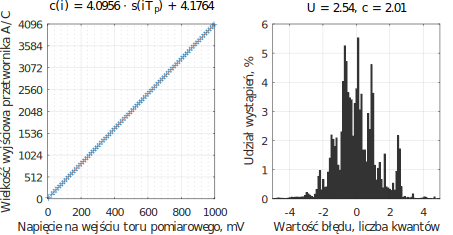
\includegraphics{obrazki/static_adcout}
\makecaption{fig:pom_static_fun}{Zależność wartości wielkości wyjściowej przetwornika analogowo-cyfrowego w funkcji wartości napięcia wejściowego analizowanego toru pomiarowego oraz histogram uzyskanych realizacji błędu losowego wielkości wyjściowej przetwornika analogowo-cyfrowego}
\end{center}
\end{figure}

Wykonany eksperyment pozwolił na identyfikację wypadkowego błędu przesunięcia zera wzmacniacza pomiarowego oraz przetwornika analogowo cyfrowego, który w analizowanym przypadku wyniósł \qty{0.123}{mV}. Błąd ten korygowany jest na etapie odtwarzania wartości wielkości $x(i)$ w przypadku warunków otoczenia identycznych do panujących podczas przeprowadzania eksperymentu. Na podstawie dokumentacji zastosowanych komponentów w rozważaniach należy uwzględnić zależność realizacji omawianego sygnału błędu w funkcji temperatury otoczenia. W przypadku wzmacniacza pomiarowego czułość błędu zera w funkcji temperatury otoczenia wynosi typowo \qty{\pm 2}{\micro V \per K} dla wzmocnienia statycznego na poziomie \qty{1}{V \per V}. W przypadku przetwornika analogowo-cyfrowego wartość ta nie jest przedstawiona w dokumentacji, natomiast producent układu proponuje wykonanie procedury kalibracji, a następnie na jej podstawie wykonywanie korekcji błędu przesunięcia zera stosując wbudowany przetwornik temperatury. Jako, że wszystkie eksperymenty związane z pracą przeprowadzane były przy stałej temperaturze otoczenia wynoszącej \qty{21}{\degreeCelsius}, analiza opisywanych zjawisk została pominięta. W przypadku zmiany wartości temperatury otoczenia należy przeprowadzić odpowiedni eksperyment mający na celu identyfikację czułości sygnału błędu związanego z dryfem zera w funkcji temperatury otoczenia, a następnie korygować należy wyniki pomiaru lub uwzględniać udział omawianego sygnału błędu w budżecie niepewności. 

Analizując dokumentacje~\cite{microchip_manual, stm_manual, diodes_manual, stm_f411} kolejnych komponentów toru pomiarowego zauważyć można, że najistotniejsze źródło błędów związanych z właściwościami statycznymi stanowi w analizowanym przypadku przetwornik analogowo-cyfrowy. Zgodnie z dokumentacją~\cite{stm_f411}, typowa wartość błędu granicznego wielkości wyjściowej $c(i)$ dla zbliżonych do stosowanych w sporządzonej aplikacji parametrów pracy przetwornika analogowo-cyfrowego powinna mieścić się w przedziale $\pm<2; 3>~\unit{LSB}$. Najważniejsze źródła błędu, które zdefiniowane są przez producenta zastosowanego przetwornika analogowo-cyfrowego obejmują: błąd przesunięcia charakterystyki względem zera, błąd wzmocnienia, całkowy błąd nieliniowości i różnicowy błąd nieliniowości~\cite{stm_adc, stm_f411}. Uzyskana na drodze eksperymentu wartość niepewności rozszerzonej jest mniejsza od wartości wynikającej z opisanego w dokumentacji błędu granicznego ze względu na fakt, że skorygowany został błąd zera oraz błąd wzmocnienia. Przeprowadzony eksperyment pozwolił zidentyfikować wypadkowe parametry sumy opisanych sygnałów błędów, przy czym należy zauważyć, że ze względu niewielką w stosunku do rozdzielczości przetwornika liczbę serii pomiarowych, nie udało się uzyskać większości realizacji różnicowego błędu nieliniowości. Na podstawie wyników eksperymentu oraz informacji zawartych w dokumentach~\cite{stm_f411, stm_adc} można jednak przyjąć, że wartość niepewności $U_{c,rw}$ została oszacowana prawidłowo. Ze względu na niewielką liczbę realizacji różnicowego błędu nieliniowości można zakładać, że rzeczywisty rozkład błędu $e_{c,rw}(i)$ będzie rozkładem normalnym, co wynika z centralnego twierdzenia granicznego~\cite{jcgm_guide}.

Drugą grupę właściwości stanowią właściwości dynamiczne. Podobnie, jak w przypadku właściwości statycznych, istnieje możliwość ich identyfikacji pomiarowej, uzyskując kolejne realizacje wielkości wyjściowej $c(i)$. Przypadek właściwości dynamicznych jest jednak złożony i wymaga stosowania bardziej skomplikowanej procedury pomiarów -- konieczna bowiem jest odpowiednia synchronizacja przebiegu napięcia wejściowego toru pomiarowego z przebiegiem sygnału wyjściowego przetwornika analogowo-cyfrowego, w celu oszacowania różnicy pomiędzy fazami analizowanych sygnałów. Opisywana procedura jest zatem kłopotliwa, a dodatkowo podczas jej realizacji wprowadzany byłby kolejny błąd, związany z opisywaną synchronizacją. Wobec powyższych okoliczności proponuje się w pierwszej kolejności identyfikację właściwości dynamicznych zastosowanego wzmacniacza pomiarowego, a następnie ustalenie właściwości dynamicznych przetwornika analogowo-cyfrowego na podstawie jego dokumentacji~\cite{stm_f411}, która szczegółowo opisuje model tego przetwornika.

W przypadku wzmacniacza pomiarowego proponowana procedura identyfikacji jego właściwości polega na podawaniu na wejście analizowanego wzmacniacza napięcia sinusoidalnie zmiennego o zadanej pulsacji i stałej amplitudzie. Dla zadanych parametrów sygnału wejściowego $s(t)$ zmierzyć należy amplitudę sygnału wyjściowego $y(t)$ wzmacniacza, potrzebną do wyznaczenia jego wzmocnienia $K_{y}(\omega)$, oraz przesunięcie fazowe $\varphi_{y}(\omega)$ pomiędzy sygnałem wejściowym i wyjściowym. Pomiędzy omawianymi wielkościami zachodzą następujące relacje:
\begin{gather}
K_{y} \emb{\omega} = \frac{E_{wy} \emb{\omega}}{E_{we} \emb{\omega}} \label{eq:pom_dyn_amp}, \\
\varphi_{y} \emb{\omega} = \varphi_{wy} \emb{\omega} - \varphi_{we} \emb{\omega} = -\omega \cdot \Delta t \emb{\omega} \label{eq:pom_dyn_phi},
\end{gather}
gdzie w funkcji pulsacji $E_{wy}(\omega)$ jest amplitudą sygnału wyjściowego, $E_{we}(\omega)$ amplitudą sygnału wejściowego, $\varphi_{wy}(\omega)$ przesunięciem fazowym sygnału wyjściowego, $\varphi_{we}(\omega)$ przesunięciem fazowym sygnału wejściowego wzmacniacza, natomiast $\Delta t(\omega)$ opóźnieniem sygnału wyjściowego względem sygnału wejściowego.

Omawiany eksperyment przeprowadzono wykorzystując jako źródło napięcia wejściowego analizowanego wzmacniacza generator przebiegów arbitralnych RIGOL DG1011~\cite{rigol_fawg}. W celu oszacowania wartości parametrów opisanych równaniami~\eqref{eq:pom_dyn_amp} oraz~\eqref{eq:pom_dyn_phi} zastosowano oscyloskop RIGOL DS5062MA~\cite{rigol_dso} w połączeniu z dwiema identycznymi sondami P6100~\cite{wellzion_probes}. Ze względu na zastosowanie dwóch identycznych sond pomiarowych obecne w zmierzonym wzmocnieniu i przesunięciu fazowym błędy były identyczne dla obydwóch kanałów, a zatem w równaniach~\eqref{eq:pom_dyn_amp} oraz~\eqref{eq:pom_dyn_phi} wzajemnie się kompensowały. Ze względu na pomiar amplitudy sygnału zarówno dla napięcia wejściowego, jak i wyjściowego analizowanego wzmacniacza, ewentualna rozbieżność nastawy wartości amplitudy napięcia wyjściowego generatora była nieistotna. Ze względu na bardzo małą wartość błędu nastawy częstotliwości przyjmuje się, że rzeczywista wartość częstotliwości sygnału wyjściowego generatora jest równa wartości zadanej tej częstotliwości. Podczas pomiarów analizowano uśrednione wartości dla $256$ realizacji obserwowanych sygnałów.

Na podstawie pozyskanych danych oszacowano pasmo przenoszenia analizowanego wzmacniacza, któremu dla zastosowanej konfiguracji układu odpowiadała częstotliwość graniczna $f_{y,g} \approx \qty{175}{kHz}$ oraz wzmocnienie statyczne $s_{y,a} \approx \qty{3.3}{V \per V}$. Dla przedstawionych charakterystyk sporządzono dwa modele, mające na celu przybliżenie właściwości analizowanego obiektu w zakresie częstotliwości $f \in~<0;\frac{1}{2}f_{p}>$. W modelu pierwszym wykorzystano funkcję opisującą transmitancję wzmacniacza w postaci:
\begin{gather}
\tilde{G}_{y,a} \emb{j\omega} = \frac{s_{y,a}}{1 + j \frac{\omega}{2 \pi f_{y,g}}} = \frac{s_{y,a}}{\frac{\omega^{2}}{4 \pi^{2} f_{y,g}^{2}} + 1} - j \frac{\omega s_{y,a}}{2 \pi f_{y,g} \left( \frac{\omega^{2}}{4 \pi^{2} f_{y,g}^{2}} + 1 \right) } \label{eq:pom_dyn_trans},
\end{gather}
natomiast dla modelu drugiego wykonano metodą najmniejszych kwadratów aproksymacje wielkości opisanych równaniami~\eqref{eq:pom_dyn_amp} oraz~\eqref{eq:pom_dyn_phi} przy użyciu funkcji:
\begin{gather}
\tilde{K}_{y,b} \emb{\omega} = 3.395 - 0.125 \exp \emb{\num{1.789e-6} \omega} \label{eq:pom_aprox_amp}, \\
\tilde{\varphi}_{y,b} \emb{\omega} = -\frac{1.700 \omega^{5}}{\num{e30}} + \frac{6.517 \omega^{4}}{\num{e24}} - \frac{7.932 \omega^{3}}{\num{e18}} + \frac{2.921 \omega^{2}}{\num{e12}} - \frac{6.924 \omega}{\num{e07}} \label{eq:pom_aprox_phi}.
\end{gather}
Uzyskane dla sygnału o częstotliwościach z zakresu $f \in~<0.1; 24>~\unit{kHz}$ wartości wzmocnienia i przesunięcia fazowego oraz odpowiadające im aproksymacje dla modeli opisanych w równaniach od~\eqref{eq:pom_dyn_trans} do~\eqref{eq:pom_aprox_phi} przedstawiono na rysunku~\ref{fig:pom_dynamic_ampout}.

\begin{figure}[htb!]
\begin{center}
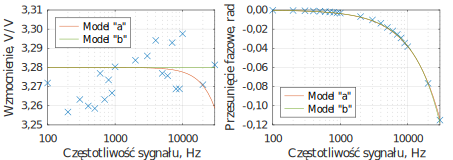
\includegraphics{obrazki/dynamic_ampout}
\makecaption{fig:pom_dynamic_ampout}{Zależność wartości wzmocnienia oraz przesunięcia fazowego w funkcji częstotliwości dla zastosowanej konfiguracji wzmacniacza pomiarowego}
\end{center}
\end{figure}

Analizując przedstawione wykresy zauważyć można, że model zaproponowany w równaniach~\eqref{eq:pom_aprox_amp} oraz~\eqref{eq:pom_aprox_phi} stanowi akceptowalne przybliżenie charakterystyki analizowanego wzmacniacza pomiarowego, natomiast model dany równaniem~\eqref{eq:pom_dyn_trans} odbiega od niej znacząco, przez co nie może być stosowany. Wobec powyższych przyjmuje się, że równania~\eqref{eq:pom_aprox_amp} oraz~\eqref{eq:pom_aprox_phi} opisywać będą właściwości dynamiczne zastosowanego wzmacniacza, odpowiadające zależnościom~\eqref{eq:mid_cont_amp} oraz~\eqref{eq:mid_cont_phi}, a zatem zachodzi $\tilde{K}_{y}(\omega) = \tilde{K}_{y,b}(\omega)$ oraz $\tilde{\varphi}_{y}(\omega) = \tilde{\varphi}_{y,b}(\omega)$. Należy zauważyć, że na potrzeby zaproponowanego w pracy modelu błędu pozyskane w wyniku przeprowadzonego eksperymentu informacje będą wystarczające i nie jest konieczna znajomość dokładnej postaci funkcji opisującej transmitancję analizowanego obiektu.

Ostatni etap identyfikacji właściwości dynamicznych obejmuje właściwości przetwornika analogowo-cyfrowego. Zgodnie z dokumentacją~\cite{stm_f411} obwód zastępczy części analogowej przetwornika analogowo-cyfrowego przedstawić można w postaci modelu filtra dolno-przepustowego typu \enquote{RC}, przy czym stanowić on będzie kaskadowe połączenie dwóch takich filtrów, co przedstawiono na rysunku~\ref{fig:pom_schemat_adc}. Wypadkowa pojemność $C_{we}$ wynika w analizowanym przypadku z pojemności w obrębie wyprowadzenia mikrokontrolera, natomiast pojemność $C_{adc}$ wynika pojemności wewnętrznej układu próbkująco-pamiętającego. Zgodnie z dokumentacją wewnętrzna pojemność przetwornika wynosi typowo około~\qty{4}{pF}, natomiast pojemność zastępcza $C_{we}$ obwodu wejściowego przetwornika wynosi zwykle około~\qty{5}{pF}. Rezystancję $R_{we}$ w zaproponowanym modelu stanowi szeregowe połączenie rezystancji doprowadzeń pomiędzy wzmacniaczem pomiarowym i mikrokontrolerem oraz rezystancji wyjściowej wzmacniacza, przy czym w omawianym przypadku jest to wartość rzędu pojedynczych Ohmów. Rezystancja $R_{adc}$ jest rezystancją klucza układu próbkująco-pamiętającego i, zgodnie z dokumentacją, jej wartość nie przekracza~\qty{6}{k\ohm}. Dodatkowe elementy, które można zauważyć na omawianym schemacie, to diody zabezpieczające wejście mikrokontrolera przed zbyt wysokim lub zbyt niskim napięciem wejściowym oraz źródło $I_{adc}$, które zastępuje upływność układu nieprzekraczającą~\qty{\pm 1}{\micro A}. Elementy te mogą być pominięte w omawianej analizie, ze względu na ich znikome znaczenie w budżecie błędów analizowanego toru pomiarowego.

\begin{figure}[htb!]
\begin{center}
\includegraphics{obrazki/schemat_adc}
\makecaption{fig:pom_schemat_adc}{Schemat zastępczy modelu przetwornika analogowo-cyfrowego zastosowanego w analizowanym torze pomiarowym zgodny z dokumentacją producenta układu~\cite{stm_f411}}
\end{center}
\end{figure}

Pierwszy filtr, który przedstawiono na rysunku~\ref{fig:pom_schemat_adc}, składa się z rezystancji rzędu pojedynczych Ohmów oraz pojemności rzędu mikro Faradów. Pozwala to oszacować częstotliwość graniczną tego filtru na poziomie kilkuset giga Herców. Filtr drugi stanowi połączenie rezystancji rzędu kilo Ohmów z pojemnością rzędu piko Faradów, a zatem rząd wielkości częstotliwości granicznej takiego filtru oszacować można na poziomie kilkuset mega Herców. Na podstawie przedstawionych parametrów modelu analizowanego przetwornika analogowo-cyfrowego, przyjąć można pomijalnie mały udział jego właściwości dynamicznych w puli właściwości dynamicznych całego toru pomiarowego. Ostateczna analiza właściwości dynamicznych całości toru pomiarowego uwzględniać może jedynie właściwości dynamiczne zastosowanego wzmacniacza pomiarowego, którego pasmo przenoszenia jest znacznie niższe.

Ostatnim fragmentem toru pomiarowego, który wprowadzać może do sygnału wyjściowego dodatkowe błędy, jest algorytm dyskretnej transformacji falkowej. Przeprowadzone wcześniej badania, których wyniki przedstawiono w tabeli~\ref{tab:varnum_spline4_4_5_f32}, pozwalają przypuszczać, że wariancja błędu związanego z zaokrągleniami nie przekroczy w bieżącym przypadku rzędu piko woltów, a zatem niepewność rozszerzona z nią związana nie powinna przekroczyć rzędu mikro woltów. Oznacza to, że błędy własne zastosowanego algorytmu dyskretnej transformacji falkowej mogą być pominięte w budżecie niepewności, bez większego wpływu na oszacowaną wartość niepewności rozszerzonej wielkości wyjściowych analizowanego toru pomiarowego~\cite{jcgm_guide}.

Należy zaznaczyć, że z punktu widzenia proponowanego modelu błędu dokładna znajomość postaci funkcji przetwarzania statycznego każdego elementu toru pomiarowego nie jest znana. Przykładowo, pomimo udziału funkcji przetwarzania $f_{y}(x)$ wzmacniacza pomiarowego w równaniach~\eqref{eq:pom_func_static} oraz~\eqref{eq:pom_funx_static}, znajomość tej funkcji nie jest konieczna podczas omawianej analizy. Dodatkowo, na podstawie treści przedstawionych równań zauważyć można, że na etapie przetwarzania wielkości $c(i)$ wprowadzane jest przesunięcie charakterystyki statycznej, spowodowane błędem zera wzmacniacza pomiarowego i przetwornika analogowo-cyfrowego. Opisywana sytuacja powoduje, że funkcja przetwarzania nie spełnia właściwości addytywności, przez co nie jest możliwa analiza każdego sygnału błędu z osobna, jak proponowano w opisanym w pracy modelu błędu. Przeprowadzenie analizy z punktu widzenia wielkości wejściowej algorytmu dyskretnej transformacji falkowej umożliwia eliminację opisywanych niedogodności i wykorzystanie równań od~\eqref{eq:out_disc_err_stat_self} do~\eqref{eq:out_disc_err_rand_prop}, umożliwiających analizę z zastosowaniem metody superpozycji dla obecnych w torze pomiarowym sygnałów.

\section{Model błędu toru pomiarowego}

Przyjmując założoną wcześniej czułość dla wielkości $x(i)$ w stosunku do przetwarzanego sygnału $s(t)$ równą $s_{s,x} = \qty{1}{V \per V}$, idealny oraz zakłócony sygnałem błędu przebieg wielkości $x(i)$ opisać można w postaci:
\begin{gather}
\dot{x} \emb{i} = s_{s,x} \dot{s} \emb{kT_{p}} = \dot{s} \emb{kT_{p}} \label{eq:pom_dwtina_ideal}, \\
\tilde{x} \emb{i} = \dot{s} \emb{kT_{p}} + e_{x,\Sigma} \emb{i} \label{eq:pom_dwtina_real}.
\end{gather}
Należy zauważyć, że sygnał błędu $e_{x,\Sigma}(t)$ zawierać będzie składowe związane z właściwościami statycznymi oraz dynamicznymi analizowanego toru pomiarowego, przy czym z osobna rozpatrywane będą sygnały związane z błędami własnymi, wprowadzanymi przez obiekt, oraz propagowanymi z wejścia na wyjście obiektu.

Uwzględniając założenie odnośnie czułości wielkości $x(i)$ względem sygnału $s(t)$ wynikające z wartości wzmocnienia statycznego $\tilde{K}_{y}(0)$ oraz postaci funkcji odtwarzania statycznego danych w równaniach~\eqref{eq:pom_funx_static} oraz~\eqref{eq:pom_aprox_amp} przyjmuje się, że wzmocnienie dla wielkości $x(t)$ względem wielkości $s(t)$ wprowadzane przez wzmacniacz pomiarowy wynosi w zakresie częstotliwości $f \in~<0; \frac{1}{2} f_{p}>$:
\begin{equation}
\tilde{K}_{s,x} \emb{\omega} = \frac{\tilde{K}_{y} \emb{\omega}}{\tilde{K}_{y} \emb{0}} \cong \qty{1}{V \per V} \label{eq:pom_dwtin_amp}.
\end{equation}
Na podstawie wypadkowych właściwości dynamicznych obiektu, wynikających z właściwości wzmacniacza oraz przetwornika analogowo-cyfrowego, można natomiast przyjąć, że przesunięcie fazowe sygnału $x(i)$ względem sygnału $s(t)$ jest dane zależnością:
\begin{equation}
\tilde{\varphi}_{s,x} \emb{\omega} = \tilde{\varphi}_{y} \emb{\omega} = -\frac{1.700 \omega^{5}}{\num{e30}} + \frac{6.517 \omega^{4}}{\num{e24}} - \frac{7.932 \omega^{3}}{\num{e18}} + \frac{2.921 \omega^{2}}{\num{e12}} - \frac{6.924 \omega}{\num{e07}} \label{eq:pom_dwtin_phi}.
\end{equation}

Pierwszy składnik zawarty w sygnale błędu $e_{x,\Sigma}(t)$ stanowi sygnał związany ze zidentyfikowanymi właściwościami statycznymi analizowanego wcześniej fragmentu toru pomiarowego, opisany dla warunków wykonanego eksperymentu równaniem~\eqref{eq:pom_funx_error}. Jako, że deterministyczna postać omawianego sygnału błędu nie jest znana oraz wartości jego realizacji nie zależą od częstotliwości przetwarzanego sygnału, przyjmuje się, że sygnał ten zalicza się do puli błędów losowych własnych. Niepewność rozszerzona związana z omawianym sygnałem błędu wynosi, zgodnie z poprzednimi rozważaniami, $U_{x,rw} = \qty{0.62}{mV}$ oraz przyjmuje się normalny rozkład realizacji tego błędu.

Drugi składnik sygnału błędu $e_{x,\Sigma}(t)$ stanowi sygnał związany z właściwościami dynamicznymi wzmacniacza pomiarowego, przy czym błąd ten ma charakter deterministyczny i można podzielić go na sygnał związany z błędem własnym oraz propagowanym. Analizując założenie opisane równaniem~\eqref{eq:pom_dwtin_amp} oraz charakterystykę amplitudową przedstawioną na rysunku~\ref{fig:pom_dynamic_ampout} zauważyć można, że dla zakresu częstotliwości $f \in~<0; \frac{1}{2} f_{p}>$ wartość wzmocnienia $\tilde{K}_{s,x}(\omega)$ jest stała, a zatem parametr ten nie ma wpływu na wprowadzane i przetwarzane sygnały błędów dynamicznych. Wobec powyższych, zgodnie z równaniami~\eqref{eq:mid_disc_err_dyn_self}, \eqref{eq:mid_disc_err_dyn_prop}, \eqref{eq:pom_funx_static} oraz~\eqref{eq:pom_dwtin_amp}:
\begin{gather}
\begin{split}
e_{x,dw} \emb{i} =~
& \sum _{j = 1} ^{\infty} E_{s,o} \emb{\omega_{x,j}} \sin \left( \omega_{s,j} iT_{p} + \varphi_{s,o} \emb{\omega_{s,j}} + \tilde{\varphi}_{s,x} \emb{\omega_{s,j}} \right) - \\
& \sum _{k = 1} ^{\infty} E_{s,o} \emb{\omega_{x,k}} \sin \left( \omega_{s,k} iT_{p} + \varphi_{s,o} \emb{\omega_{s,k}} + \dot{\varphi}_{s,x} \emb{\omega_{s,k}} \right)
\end{split}
\label{eq:pom_errx_dyn_self}, \\
e_{x,dp} \emb{i} = \sum _{j = 1} ^{\infty} E_{s,e} \emb{\omega_{s,j}} \sin \left( \omega_{s,j} iT_{p} + \varphi_{s,e} \emb{\omega_{s,j}} + \tilde{\varphi}_{s,x} \emb{\omega_{s,j}} \right) \label{eq:pom_errx_dyn_prop},
\end{gather}
przy czym stosowane oznaczenia parametrów sygnału $s(t)$ są zbieżne z tymi wprowadzonymi w równaniach od~\eqref{eq:in_cont_sum_ideal} do~\eqref{eq:in_cont_err_dyn} oraz $\dot{\varphi}_{s,x}(\omega) = \qty{0}{rad}$.

Trzeci składnik sygnału błędu $e_{x,\Sigma}(t)$ wynika z wpływu analizowanego obiektu na obecny w przetwarzanym sygnale $s(t)$ sygnał błędu statycznego $e_{s,s}(t)$, przy czym przebieg tego sygnału na wyjściu obiektu opisać można zgodnie z równaniem~\eqref{eq:pom_funx_static} jako:
\begin{equation}
e_{x,sp} \emb{i} = e_{s,s} \emb{i T_{p}} \label{eq:pom_errx_stat_prop}.
\end{equation}
Oznacza to, że zgodnie z równaniami~\eqref{eq:mid_disc_var_omega} oraz~\eqref{eq:out_disc_var_sense}, wariancję tego sygnału opisać można następującą zależnością:
\begin{equation}
\sigma_{x,sp}^{2} = s_{s,x}^{2} \tilde{K}_{s,x}^{2} \emb{0} \sigma_{s,s}^{2} \cong \sigma_{s,s}^{2} \label{eq:pom_varx_stat_prop}.
\end{equation}
Jako, że przeprowadzone eksperymenty wykonano przy stałych parametrach otoczenia, nie obejmowały one identyfikacji źródeł i postaci sygnału błędu statycznego własnego. Przyjmuje się zatem, że $e_{x,sw}(i) = 0$ oraz $\sigma_{x,sw}^{2} = 0$.

Czwartym składnikiem sygnału błędu $e_{x,\Sigma}(t)$ jest propagowany sygnał błędu losowego $e_{s,r}(t)$. Zgodnie z zależnościami~\eqref{eq:mid_disc_var_omega} oraz~\eqref{eq:out_disc_var_sense} dla założenia danego równaniem~\eqref{eq:pom_dwtin_amp} wariancję tego sygnału opisać można w postaci:
\begin{equation}
\sigma_{x,rp}^{2} = s_{s,x}^{2} \tilde{K}_{s,x}^{2} \emb{\omega} \sigma_{s,r}^{2} \emb{\omega} \cong \sigma_{s,r}^{2} \emb{\omega} \label{eq:pom_varx_rand_prop},
\end{equation}
co przy założeniu~\eqref{eq:pom_dwtina_ideal} odnośnie liniowości tego obiektu oznacza, że obiekt ten nie ma wpływu na widmo sygnałów losowych w zakresie częstotliwości $f \in~<0; \frac{1}{2} f_{p}>$, zatem:
\begin{equation}
e_{x,rp} \emb{i} \cong e_{x,r} \emb{i} \cong e_{s,r} \emb{i T_{p}} \label{eq:pom_errx_rand_prop}.
\end{equation}
W przypadku sygnału losowego błędu własnego $e_{x,rw}(i)$ przeprowadzony eksperyment pozwolił oszacować wariancję tego sygnału $\sigma_{x,rw}^{2} = \qty{0.095}{\micro V}$ oraz związaną z nią niepewność $U_{x,rw} = \qty{0.62}{mV}$, gdzie zakłada się $c_{x,rw} = c_{n} = 1.96$.

Na podstawie zależności od~\eqref{eq:pom_dwtina_ideal} do~\eqref{eq:pom_errx_rand_prop} wypadkowy sygnał błędu $e_{x,\Sigma}(t)$ opisać można jako sumę zdefiniowanych dotychczas sygnałów błędów cząstkowych w postaci:
\begin{equation}
e_{x,\Sigma} \emb{i} = e_{x,sp} \emb{i} + e_{x,dw} \emb{i} + e_{x,dp} \emb{i} + e_{x,rw} \emb{i} + e_{x,rp} \emb{i} \label{eq:pom_errx_sum},
\end{equation}
przy czym wypadkowe sygnały błędów z uwzględnieniem podziału na zaproponowane kategorie można zdefiniować jako:
\begin{gather}
e_{x,s} \emb{i} = e_{x,sp} \emb{i} \label{eq:pom_errx_stat}, \\
e_{x,d} \emb{i} = e_{x,dw} \emb{i} + e_{x,dp} \emb{i} = \sum _{j=1} ^{\infty} E_{x,e} \emb{\omega_{x,j}} \sin \emb{i T_{p} \omega_{x,j} + \varphi_{x,e} \emb{\omega_{x,j}}} \label{eq:pom_errx_dyn}, \\
e_{x,r} \emb{i} = e_{x,rw} \emb{i} + e_{x,rp} \emb{i} \label{eq:pom_errx_rand},
\end{gather}
gdzie wypadkowe parametry amplitudy $E_{x,e}(\omega_{x,j})$ oraz fazy $\varphi_{x,e}(\omega_{x,j})$ dla kolejnych harmonicznych sygnału wypadkowego błędu dynamicznego $e_{x,d}(i)$ zależne będą od widma przetwarzanego sygnału, natomiast ich wyznaczenie przebiegać będzie zgodnie z metodologią opisaną w równaniach od~\eqref{eq:dyn_vect} do~\eqref{eq:dyn_vect_phi}. Wariancję kolejnych harmonicznych sygnału $e_{x,d}(i)$ wyznaczyć można zgodnie z zależnością~\eqref{eq:dyn_var}.

Przedstawiona aplikacja zaproponowanego w pracy modelu błędu wielkości wejściowych algorytmu dyskretnej transformacji falkowej umożliwia określenie wariancji każdego z wymienionych w równaniu~\eqref{eq:pom_errx_sum} sygnałów oraz wyznaczenie niepewności rozszerzonej związanej z tymi sygnałami. W przypadku sygnałów błędów statycznych i losowych dla $i-tej$ wielkości wyjściowej toru pomiarowego zachodzi:
\begin{gather}
\sigma_{i,s}^{2} = \left| H_{i} \emb{0} \right|^{2} = A_{i,s}^{2} \sigma_{x,s}^{2} \label{eq:pom_varout_stat}, \\
\sigma_{i,r}^{2} = A_{i,r}^{2} \sigma_{x,r}^{2} \label{eq:pom_varout_rand}, 
\end{gather}
co wynika bezpośrednio z zależności opisanych równaniami od~\eqref{eq:alg_outvar_stat} do~\eqref{eq:alg_outvar_trans_rand} oraz założenia dotyczącego stałej widmowej gęstości mocy w przypadku sygnałów błędu kwantowania i wypadkowego błędu niedoskonałości charakterystyki statycznej. W przypadku sygnałów błędów dynamicznych, wariancję tych sygnałów w funkcji pulsacji opisać można równaniem:
\begin{equation}
\sigma_{i,d}^{2} \emb{\omega} = \left| H_{i} \emb{\omega T_{p}} \right|^{2} \sigma_{x,d}^{2} \emb{\omega} \label{eq:pom_varout_dyn},
\end{equation}
natomiast wypadkowa wariancja sygnału błędu dynamicznego może zostać opisana w postaci sumy wypadkowych wariancji wszystkich harmonicznych tego sygnału:
\begin{equation}
\sigma_{i,d}^{2} = \sum _{j=1} ^{\infty} \left| H_{i} \emb{\omega_{x,j} T_{p}} \right|^{2} \sigma_{x,d}^{2} \emb{\omega_{x,j}} \label{eq:pom_varout_dyn_sum}.
\end{equation}
Należy zauważyć, że na etapie analizy kolejnych harmonicznych sygnału błędu dynamicznego $e_{x,d}(i)$ kolejne harmoniczne tego sygnału mogą być ze sobą skorelowane. Proponowane w równaniu~\eqref{eq:pom_errx_dyn} przedstawienie tego sygnału w postaci kolejnych harmonicznych o parametrach wypadkowych umożliwia rozpatrzenie tych korelacji przy jednoczesnej redukcji liczby składowych analizowanego sygnału. Ze względu na to, że przeprowadzona identyfikacja właściwości metrologicznych dla fragmentu toru pomiarowego związanego z wielkościami wejściowymi analizowanego algorytmu nie wykazała innych korelacji pomiędzy zidentyfikowanymi sygnałami błędów, zgodnie z równaniem~\eqref{eq:var_matrix} zapisać można:
\begin{equation}
\sigma_{i,\Sigma}^{2} = \sigma_{i,s}^{2} + \sigma_{i,d}^{2} + \sigma_{i,r}^{2} \label{eq:pom_varout_sum}.
\end{equation}
Wartości wariancji sygnałów propagowanego błędu statycznego, propagowanego błędu losowego oraz wypadkowego błędu dynamicznego nie są znane na obecnym etapie analizy. Dla wymienionych sygnałów wartość wariancji zależeć będzie od widma sygnału $s(t)$ oraz zawartych w nim sygnałów błędów.

Wartości niepewności rozszerzonych związane z wymienionymi sygnałami błędów na wyjściu algorytmu mogą być w analizowanej sytuacji opisane jako:
\begin{gather}
U_{i,s} = c_{x,s} \sigma_{i,s} \label{eq:pom_uncout_stat}, \\
U_{i,d,j} = c_{d} \sigma_{i,d} \emb{\omega_{x,j}} \label{eq:pom_uncout_dyn}, \\
U_{i,r} = c_{n} \sigma_{i,r} \label{eq:pom_uncout_rand},
\end{gather}
gdzie zgodnie ze zidentyfikowanymi właściwościami obiektu $c_{x,s} = c_{n} = 1.96$. Wartość współczynnika rozszerzenia w przypadku sygnału błędu losowego na wyjściu obiektu wynika z założeń centralnego twierdzenia granicznego, gdzie analizowany algorytm przetwarza wiele nieskorelowanych ze sobą sygnałów błędów losowych o jednakowych parametrach. Wobec powyższych, wypadkowa wartość niepewności rozszerzonej na wyjściu algorytmu dla $i$-tej wielkości wyjściowej może być opisana zgodnie z równaniem~\eqref{eq:unc_matrix}, przy czym w analizowanym przypadku wektor niepewności sygnałów składowych opisać można jako:
\begin{equation}
\mathbf{U}_{i}^{T} = 
\begin{bmatrix}
U_{i,s} & U_{i,r} & U_{i,d,1} & U_{i,d,2} & \hdots & U_{i,d,K}
\end{bmatrix}
\label{eq:pom_uncout_uncvect},
\end{equation}
natomiast macierz koherencji dla $K$ harmonicznych sygnału błędu dynamicznego opisać można w postaci:
\begin{equation}
\mathbf{h}_{i} =
\begin{bmatrix}
1           & h_{i,s,r}   & h_{i,s,d,1} & h_{i,s,d,2} & \cdots & h_{i,s,d,K} \\
h_{i,r,s}   & 1           & h_{i,r,d,1} & h_{i,r,d,2} & \cdots & h_{i,r,d,K} \\
h_{i,d,1,s} & h_{i,d,1,r} & 1           & h_{i,d,1,2} & \cdots & h_{i,d,1,K} \\
h_{i,d,2,s} & h_{i,d,2,r} & h_{i,d,2,1} & 1           & \cdots & h_{i,d,2,K} \\
\vdots      &             &             &             & \ddots & \vdots      \\
h_{i,d,K,1} & \cdots      & \cdots      & \cdots      & \cdots & 1           \\
\end{bmatrix}
\label{eq:pom_uncout_cohers},
\end{equation}
gdzie kolejne wartości współczynników koherencji są wyznaczane zgodnie z równaniem~\eqref{eq:unc_coher}. Wobec przedstawionych założeń, wartość wypadkowej niepewności rozszerzonej dla analizowanego przypadku wynosi:
\begin{equation}
U_{i,\Sigma} = \sqrt{\mathbf{U}_{i}^{T} \mathbf{h}_{i} \mathbf{U}_{i}} \label{eq:pom_uncout_sum}.
\end{equation}
Zgodnie z założeniami odnośnie bardzo niskiej w stosunku do pozostałych sygnałów wariancji błędu własnego zaokrągleń, udział tego błędu pominięto w rozważaniach.

\section{Przypadek sygnału monoharmonicznego}

Pierwszym rozważanym eksperymentem jest weryfikacja poprawności przedstawionej aplikacji modelu błędu dla przypadku, kiedy analizowany tor pomiarowy przetwarza opisany równaniem~\eqref{eq:pom_gen_out_ideal} sinusoidalnie zmienny sygnał napięciowy. Eksperyment obejmuje dwa przypadki -- dla przypadku pierwszego nieznane są rzeczywiste wartości napięcia amplitudy $\tilde{E}_{s,o}$ oraz składowej stałej $\tilde{D}_{s,o}$ przetwarzanego sygnału $s(t)$, natomiast przypadek drugi zakłada znajomość tych parametrów, pozyskaną przy użyciu dodatkowego multimetru. Należy zaznaczyć, że w przypadku znajomości rzeczywistych parametrów przetwarzanego sygnału, wyznaczone analitycznie wartości wariancji oraz wypadkowej niepewności rozszerzonej dla kolejnych wielkości wyjściowych toru pomiarowego powinny być zbieżne z uzyskanymi na drodze eksperymentu. W przypadku analizy obejmującej nieznane rzeczywiste wartości parametrów sygnału $s(t)$ uzyskane analityczne wyniki powinny dotyczyć $95\%$ egzemplarzy stosowanego generatora przebiegów arbitralnych, a zatem ich wartości powinny być co najmniej takie, jakie uzyskano w eksperymencie.

W dalszej części przyjmuje się, że opisany równaniem~\eqref{eq:pom_gen_out_ideal} przebieg $s(t)$ w przypadku idealnym cechuje amplituda $\dot{E}_{s,o} = \qty{475}{mV}$ oraz składowa stała $\dot{D}_{s,o} = \qty{500}{mV}$, natomiast wartość pulsacji $\omega_{s,o}$ zależna jest od iteracji przeprowadzonego eksperymentu. Można zatem, na podstawie równań~\eqref{eq:pom_gen_shferr_unc} oraz~\eqref{eq:pom_gen_err_dyn_mono} wskazać graniczną wartość amplitudy sygnału błędu dynamicznego $e_{s,d}(t)$ dla analizowanych warunków eksperymentu:
\begin{equation}
E_{s,e,1} = U_{E} \emb{\dot{E}_{s,o}} = \frac{1.65}{\sqrt{3}} \emb{\num{5e-3} \cdot 0.475 + \num{0.5e-3}} = \qty{2.74}{mV} \label{eq:pom_mono_dyn_amp_in}.
\end{equation}
Na podstawie treści równania~\eqref{eq:pom_errx_dyn_prop} określić można amplitudę oraz fazę analizowanego sygnału błędu na wejściu algorytmu dyskretnej transformacji falkowej:
\begin{gather}
E_{x,ep,1} \cong E_{s,e,1} \label{eq:pom_mono_dyn_prop_amp_mid}, \\
\varphi_{x,ep,1,a} = \tilde{\varphi}_{s,x} \emb{\omega_{s,o}} + \left. \varphi_{s,e,1} \right|_{\tilde{E}_{s,o} - \dot{E}_{s,o} > 0} = \tilde{\varphi}_{s,x} \emb{\omega_{s,o}} \label{eq:pom_mono_dyn_prop_phi_mid_a}, \\
\varphi_{x,ep,1,b} = \tilde{\varphi}_{s,x} \emb{\omega_{s,o}} + \left. \varphi_{s,e,1} \right|_{\tilde{E}_{s,o} - \dot{E}_{s,o} < 0} = \tilde{\varphi}_{s,x} \emb{\omega_{s,o}} + \pi \label{eq:pom_mono_dyn_prop_phi_mid_b},
\end{gather}
przy czym faza $\varphi_{x,ep,1,a}$ jest odpowiednia dla dodatnich realizacji błędu nastawy amplitudy sygnału, natomiast faza $\varphi_{x,ep,1,b}$ odpowiada ujemnym realizacjom tego błędu. W przypadku sygnału błędu statycznego, wynikającego z błędu nastawy wartości składowej stałej $\dot{D}_{x,o}$ niepewność związaną z tym sygnałem określa zależność:
\begin{equation}
U_{x,sp} = c_{x,sp} \sigma_{x,sp} \cong c_{s,s} \sigma_{s,s} = U_{s,s} = \frac{1.65}{\sqrt{3}} \emb{\num{5e-3} \cdot 0.5 + \num{2e-3}} = \qty{4.29}{mV} \label{eq:pom_mono_stat_unc_mid},
\end{equation}
wynikająca z treści równań od~\eqref{eq:pom_gen_err_stat} do~\eqref{eq:pom_gen_unc_stat}, \eqref{eq:pom_errx_stat_prop} oraz \eqref{eq:pom_varx_stat_prop}. Wariancja omawianego sygnału błędu, zgodnie z wymienionymi zależnościami, wynosi natomiast:
\begin{equation}
\sigma_{x,sp}^{2} \cong \sigma_{s,s}^{2} = \sigma_{D}^{2} \emb{\dot{D}_{s,o}} = \frac{1}{3} \emb{\num{5e-3} \cdot 0.5 + \num{2e-3}}^{2} = \qty{6.75}{\micro V} \label{eq:pom_mono_stat_var_mid}.
\end{equation}
Równania od~\eqref{eq:pom_mono_dyn_amp_in} do~\eqref{eq:pom_mono_stat_unc_mid} dotyczą przypadku, gdy rzeczywiste wartości parametrów $\tilde{E}_{s,o}$ oraz $\tilde{D}_{s,o}$ nie są znane. Dla znanych wartości tych parametrów przyjmuje się, że $E_{s,e,1} = \qty{0}{V}$ oraz $U_{s,s} = \qty{0}{V}$, a zatem zachodzi $\sigma_{x,sp}^{2} = \qty{0}{V}$ oraz $\sigma_{x,dp}^{2} = \qty{0}{V}$.

Na podstawie równania~\eqref{eq:pom_errx_dyn_self} wyróżnić można dwie składowe harmonicznej sygnału błędu dynamicznego własnego na wejściu algorytmu transformacji falkowej. Amplitudy oraz fazy tych harmonicznych w analizowanym przypadku opisać można jako:
\begin{gather}
E_{x,ew,1,1} = E_{x,ew,1,2} \cong \dot{E}_{s,o} \label{eq:pom_mono_dyn_self_amp_mid}, \\
\varphi_{x,ew,1,1} = \varphi_{s,o} + \tilde{\varphi}_{s,x} \emb{\omega_{s,o}} = \tilde{\varphi}_{s,x} \emb{\omega_{s,o}} \label{eq:pom_mono_dyn_self_phi_mid_1}, \\
\varphi_{x,ew,1,2} = \varphi_{s,o} + \dot{\varphi}_{s,x} \emb{\omega_{s,o}} + \pi = \pi \label{eq:pom_mono_dyn_self_phi_mid_2},
\end{gather}
gdzie na podstawie założeń danych równaniem~\eqref{eq:pom_gen_out_ideal} $\varphi_{s,o} = \qty{0}{rad}$ oraz zgodnie z założeniem~\eqref{eq:pom_dwtina_ideal} $\dot{\varphi}_{s,x}(\omega) = \qty{0}{rad}$. Zgodnie z definicją sygnału błędu dynamicznego $e_{x,d}(i)$ daną równaniem~\eqref{eq:pom_errx_dyn}, wynikającą z definicji~\eqref{eq:pom_errx_dyn_self} oraz~\eqref{eq:pom_errx_dyn_prop}, w analizowanym przypadku zapisać można:
\begin{equation}
\begin{split}
e_{x,d,*} \emb{i} =~
& E_{x,ew,1,2} \sin \emb{\omega_{s,o} + \varphi_{x,ew,1,2}} + E_{x,ew,1,1} \sin \emb{\omega_{s,o} + \varphi_{x,ew,1,1}} + \\
& E_{x,ep,1} \sin \emb{\omega_{s,o} + \varphi_{x,ep,1,*}} = E_{x,e,1,*} \sin \emb{\omega_{s,o} + \varphi_{x,e,1,*}}
\end{split}
\label{eq:pom_mono_dyn_sum_err_mid},
\end{equation}
gdzie rozpatrzyć należy obydwa przypadki amplitudy $E_{x,e,1,*}$ oraz fazy $\varphi_{x,e,1,*}$ sygnału propagowanego błędu dynamicznego $e_{x,dp}(i)$ dla wariantów parametru $\varphi_{x,ep,1,*}$, którego wartości w zależności od zaistniałych okoliczności opisano w równaniach~\eqref{eq:pom_mono_dyn_prop_phi_mid_a} oraz~\eqref{eq:pom_mono_dyn_prop_phi_mid_b}. Zgodnie z metodologią opisaną w równaniach~od~\eqref{eq:dyn_vect} do~\eqref{eq:dyn_vect_phi} wartości parametrów amplitudy $E_{x,e,1}$ oraz fazy $\varphi_{x,e,1}$ sygnału błędu dynamicznego $e_{x,d}(i)$ na wejściu algorytmu dyskretnej transformacji falkowej mogą być wyznaczone jako:
\begin{gather}
E_{x,e,1,*} = \sqrt{e_{x,1,\Sigma,a,*}^{2} + e_{x,1,\Sigma,b,*}^{2}} \label{eq:pom_mono_dyn_sum_param_amp_mid}, \\
\varphi_{x,e,1,*} = \arctan \emb{\frac{e_{x,1,\Sigma,a,*}^{2}}{e_{x,1,\Sigma,b,*}^{2}}} \label{eq:pom_mono_dyn_sum_param_phi_mid},
\end{gather}
przy czym parametry przedstawionych równań wyznaczane są zgodnie z zależnościami:
\begin{gather}
\begin{split}
e_{x,1,\Sigma,a,*} =~ & E_{x,ew,1,2} \cos \emb{\varphi_{x,ew,1,2}} + E_{x,ew,1,1} \cos \emb{\varphi_{x,ew,1,1}} + \\ & E_{x,ep,1} \cos \emb{\varphi_{x,ep,1,*}}
\end{split}
\label{eq:pom_mono_dyn_sum_param_a_mid}, \\
\begin{split}
e_{x,1,\Sigma,b,*} =~ & E_{x,ew,1,2} \sin \emb{\varphi_{x,ew,1,2}} + E_{x,ew,1,1} \sin \emb{\varphi_{x,ew,1,1}} + \\ & E_{x,ep,1} \sin \emb{\varphi_{x,ep,1,*}}
\end{split}
\label{eq:pom_mono_dyn_sum_param_b_mid}.
\end{gather}

Należy podkreślić, że rzeczywisty przebieg sygnału błędu dynamicznego własnego $e_{x,dw}(i)$ również skorelowany jest z rzeczywistą wartością amplitudy $\tilde{E}_{s,o}$. Korelacja ta jest jednak pominięta w przeprowadzonej analizie ze względu na niewielkie wartości błędu nastawy tego parametru i w efekcie niski współczynnik korelacji opisywanego zjawiska. Jest to założenie analogiczne, jak stosowanie idealnej charakterystyki przetwarzania obiektu w przypadku analizy statycznych właściwości tego obiektu.



\section{Podsumowanie przeprowadzonego eksperymentu}

TODO


\chapter{Podsumowanie pracy}

Zaproponowany w pracy model błędów umożliwia opis właściwości metrologicznych torów pomiarowych złożonych zarówno z części przetwarzania analogowego, jak i cyfrowego. Model ten obejmuje dwa rodzaje właściwości: dynamiczne -- związane z widmem przetwarzanego sygnału, oraz statyczne -- niezależne od widma przetwarzanego sygnału. Stosowanie zaproponowanego modelu błędów jest możliwe bez znajomości dokładnej struktury wewnętrznej analizowanego układu, a zatem model ten znajduje swoje zastosowanie do opisu między innymi urządzeń typu \enquote{SoC}. Parametry omówionego modelu błędów mogą być pozyskiwane na drodze eksperymentu pomiarowego, jak i szacowane na podstawie dokumentacji analizowanego urządzenia.

Opis właściwości metrologicznych analizowanego obiektu wykorzystujący miarę wariancji sygnału błędu na wyjściu tego obiektu jest znacznie bardziej przystępny z punktu widzenia skomplikowania obliczeń, niż opis wykorzystujący miarę niepewności rozszerzonej (w szczególności, gdy kolejne sygnały błędów nie są ze sobą w żaden sposób skorelowane). Opis ten nie dostarcza jednak informacji o prawdopodobieństwie uzyskania danej wartości realizacji sygnału błędu, a zatem jest mniej użyteczny, niż ten wykorzystujący miarę niepewności rozszerzonej.

Zastosowana w pracy metoda szacowania wypadkowej wartości niepewności rozszerzonej, wykorzystująca metodę redukcyjnej arytmetyki interwałowej, wraz z zaproponowaną modyfikacją zapewnia wyniki zbieżne z uzyskiwanymi metodą Monte-Carlo. Ze względu na niską złożoność obliczeniową omawianej metody, jej stosowanie jest możliwe w czasie rzeczywistym, również w przypadku zmiany parametrów modelu błędów lub widma przetwarzanego sygnału. Ograniczeniem przedstawionej metody jest konieczność wstępnego wyznaczenia wartości dla współczynników kształtu, przy czym procedura ta nie może odbywać się w czasie rzeczywistym, natomiast jest ona jednorazowa. W przypadku wystąpienia korelacji pomiędzy analizowanymi sygnałami błędów należy wyznaczyć wypadkowe wartości niepewności rozszerzonej dla skorelowanych grup sygnałów lub zastosować inną, niż zaproponowano w pracy, metodę wyznaczania wartości współczynników koherencji. Niezależnie, czy obliczenia prowadzone są z wykorzystaniem budżetu niepewności obejmującego wszystkie źródła błędów, czy stosowane są wypadkowe parametry dla wyróżnionych w pracy grup sygnałów błędów, omawiana metoda zapewnia bardzo zbliżone wyniki. Należy jednak zaznaczyć, że wyznaczanie wypadkowych wartości niepewności rozszerzonej w przypadku nietypowego kształtu rozkładu wypadkowego sygnału błędu uniemożliwia wykorzystanie wyznaczonej wartości niepewności rozszerzonej w dalszych obliczeniach. Właściwość ta spowodowana jest koniecznością znajomości wartości współczynników kształtu analizowanych par sygnałów. Jako, że wartości współczynników kształtu muszą zostać wyznaczone dla wcześniej zdefiniowanych parametrów rozkładu sygnałów, wyznaczenie wartości współczynników koherencji zgodnie z proponowaną w pracy metodą jest w omawianym przypadku niemożliwe. Należy zauważyć, że w praktyce wada ta jest nieistotna, ponieważ podczas implementacji algorytmu wykorzystującego przedstawioną metodę stosowane są odpowiednio wyprowadzone zależności, wynikające z wzajemnych relacji pomiędzy kolejnymi fragmentami toru pomiarowego, co wykazano w przedstawionych przykładach.

Przedstawienie algorytmu transformacji falkowej w postaci macierzowej umożliwia analizę właściwości metrologicznych tego algorytmu w sposób zbieżny z opisywaną w pracy metodą analizy cyfrowej cześć toru pomiarowego. Omawiany algorytm przedstawić można jako zbiór cyfrowych fragmentów toru pomiarowego, których model właściwości metrologicznych opisano w pracy. Wyznaczenie wartości współczynników macierzy transformacji dla analizowanego algorytmu odbywać się może analitycznie, na podstawie założeń dotyczących stosowanej rodziny falek, lub może zostać przeprowadzone na podstawie istniejącej implementacji tego algorytmu. Dla omawianej rodziny algorytmów istnieje również możliwość wyznaczenia wartości współczynników macierzy transformacji na podstawie transmitancji kolejnych wielkości wyjściowych algorytmu, a także przeprowadzenie operacji odwrotnej do opisanej. Jako, że w klasycznym przypadku wielkości wyjściowe algorytmu można podzielić na grupy o jednakowej transmitancji, analiza może zostać uproszczona.

Jak wykazały przeprowadzone eksperymenty, dokładność oszacowania wypadkowej wartości niepewności rozszerzonej wielkości wyjściowych analizowanego toru pomiarowego uwarunkowana jest głównie dokładnością wyznaczenia parametrów dla stosowanego modelu błędów. Z uwagi na fakt, że algorytmy transformacji falkowej stanowią zbiór filtrów, istotne jest prawidłowe oszacowanie parametrów najistotniejszych źródeł błędów dla każdej grupy sygnałów błędów: statycznych, dynamicznych oraz losowych. Nawet, jeżeli wielkości wejściowe algorytmu obarczone będą pewnym sygnałem błędu dominującego, to błąd ten może cechować się widmową gęstością mocy skoncentrowaną w okolicy częstotliwości, która dla wybranej wielkości wyjściowej jest tłumiona. W takim przypadku dla analizowanej wielkości wyjściowej przenoszone będą jedynie pozostałe sygnały błędów, przy czym sygnały te mogą być dodatkowo wzmacniane. Należy zatem zauważyć, że mimo niewielkiej rozbieżności w oszacowaniu wypadkowej wartości niepewności rozszerzonej wielkości wejściowych dla opisywanych algorytmów, wypadkowa wartość niepewności rozszerzonej na wyjściu tych algorytmów może być oszacowana niewłaściwie.

Przedstawione dotychczas wnioski podsumowujące zawarte w pracy rozważania potwierdzają założenia przedstawione we wstępie do pracy oraz sformułowaną w pracy tezę. Dalsze rozważania dotyczyć mogą uzupełniania przedstawionego modelu błędów o opis kolejnych zjawisk zakłócających proces pomiaru (np. wpływu opóźnień występujących w systemach pomiarowo-sterujących na niepewność wielkości analizowanych w tych systemach). Kolejne istotne zagadnie wymagające dalszych badań stanowi rozszerzenie opisanej w pracy metody wyznaczania wartości współczynników koherencji, obejmujące przypadki sygnałów skorelowanych, umożliwiające jednolite stosowanie omawianej metody w dowolnym przypadku.

Najważniejszy walor pracy stanowi przedstawienie jednolitego, spójnego modelu błędów umożliwiającego opis parametrów sygnałów błędów obecnych w torze pomiarowym. Zaproponowany model obejmuje etapy przetwarzania analogowego, cyfrowego oraz wskazuje wzajemne relacje pomiędzy omawianymi fragmentami. Sporządzone na potrzeby pracy podsumowanie najistotniejszych informacji dotyczących metrologicznych właściwości algorytmów transformacji falkowej umożliwia zastosowanie przedstawionego modelu błędu do opisu wpływu tych algorytmów na obecne w torze pomiarowym sygnały błędów. Istotną wartość pracy stanowi również zaproponowana metoda szacowania wypadkowej wartości niepewności rozszerzonej, przy czym metoda ta zapewnia wyniki zbliżone do tych uzyskiwanych metodą Monte-Carlo, oferując jednocześnie stosunkowo niewielką, w porównaniu do pozostałych obliczeń wykonywanych przez tor pomiarowy, złożoność obliczeniową również w przypadku zmiany wartości parametrów modelu błędów. Niniejsza praca stanowi zatem propozycję, w jaki sposób opisać można właściwości metrologiczne toru pomiarowego stosującego w swojej strukturze algorytm transformacji falkowej oraz w jaki sposób ilościowo określić niedokładność wyznaczania wartości wielkości wyjściowych tego toru. Oryginalność pracy podkreśla fakt, że dotychczas nie poruszano w literaturze problemu jednolitej analizy właściwości metrologicznych algorytmów dyskretnej transformacji falkowej.

\appendix
\end{document}

